\chapter{Pembrokeshire Welsh}
\label{cha:pembrokeshire-welsh}

This chapter deals with the analysis of certain phonological patterns in the Welsh dialect spoken in Pembrokeshire (Welsh \emph{Sir Benfro}), spoken in the south\hyp western part of Wales.

\section{Introduction}
\label{sec:introduction}

In this section I summarize the descriptive, empirical, and theoretical contribution of this chapter and describe the sources used in the work.

\subsection{The contribution}
\label{sec:contribution}

In this chapter I provide a holistic analysis of the set of phonological contrasts and alternations in a dialect of Welsh, backed up by a single representational system which is intended to account for all the patterns considered here. I leverage both the dialect description at hand and, where warranted, accounts of other varieties, to present a comprehensive approach to several phenomena which have previously been treated separately. In particular, I present new analyses of several sound patterns of Welsh, such as the following:

\begin{itemize}
\item Vowel mutation \citep{allen75:_vowel_mutat_word_stres_welsh,cartmill76:_welsh_vowel_mutat,thomas84:_north_welsh,bosch96:_promin,greenbook,hannahs07:_const_welsh}: in \cref{sec:vowel-mutation} I present a new analysis that builds on the insights of \citet{hannahs07:_const_welsh}, \citet{bosch96:_promin}, and \citet{greenbook}, although it has wider empirical scope, and propose that the pattern requires the introduction of an emergent suprasegmental feature;
\item Laryngeal features and the behaviour of \ipa{[h]} \citep{hannahs11:_welsh}: I lay out the preliminaries for an analysis of laryngeal phonology, which has so far been severely understudied (\cref{sec:laryng-assim}), and propose a unified account of the behaviour of the segment \ipa{[h]} which covers both its properties as an independent segment (previously covered by \citeauthor{hannahs11:_welsh} \cite*{hannahs11:_welsh}) and its behaviour in coalescence (\cref{sec:story-ipah});
\item Svarabhakti, \ie the treatment of word\hyp final rising\hyp sonority consonant sequences (\cf \citealp{hannahs09:_welsh}, although this covers North Welsh): in \cref{sec:evid-unev-troch} I propose a new analysis that is consistent both with the facts of South Welsh and with the overall approach to the prosodic system;
\item The behaviour of diphthongs and glides: I provide a comprehensive analysis of the phonological and phonetic behaviour of high vowels and glides in the dialect, arguing for a stricter division of labour between phonetics and phonology in this area (\cref{sec:gliding-as-phonetic}) and for a stratal analysis of those phenomena that indeed belong to the phonology (\cref{sec:cyclic-effects-lack,sec:synaresis});
\item The interaction of moraic and featural structure: finally, I provide a complete analysis of the interaction between moraic structure and segmental features in Pembrokeshire Welsh (\cref{sec:foot-intern-struct}). I show that the language exhibits a pattern of subversion of the sonority hierarchy that cannot be dealt with using \posscite{moren01:_distin} solution based on \textsc{DepLink}-\mo constraints, and propose a new account.
\end{itemize}

From the theoretical perspective, the chapter provides an extended example of the application of the theoretical principles laid out in \cref{part:theory}. For instance, I demonstrate the value of an explicit distinction between phonetics and phonology (\cref{sec:gliding-as-phonetic}) and phonology and lexical insertion (\cref{sec:status-ipau-sim,sec:evid-unev-troch}); show how representations can be used to correctly constrain the interaction of various features (\cref{sec:spec-voic-fric}); and argue for stratal analyses of several phenomena (\cref{sec:cyclic-effects-lack,sec:analysis-11,sec:synaresis}).

In addition, I make several novel theoretical proposals. First, I argue for the introduction of an emergent suprasegmental feature that interacts with subsegmental featural structure but, unlike tone, does not have a consistent phonetic expression (\cref{sec:pros-prom-as}). Second, I demonstrate that functionally arbitrary augmentation constraints have a useful rôle to play in constraining phonological patterns that would otherwise require the introduction of exhaustively interpreted markedness constraints and thus the subversion of markedness hierarchies (\cref{sec:part-mark-orders}). I provide a detailed study of two cases where augmentation constraints are useful: these involve are the licensing of laryngeal features by manner (\cref{sec:story-ipah}) and the licensing of certain feature bundles by moraicity (\cref{sec:foot-intern-struct}). In both cases I argue that analyses which do not rely on augmentation constraints either fail empirically or have a number of undesirable properties.

\subsection{Sources}
\label{sec:sources-1}

The main source is the monographic description of the dialect by \citet{awbery86:_pembr_welsh}. Since it is mainly concerned with an analysis of selected patterns, I have also used descriptions of other Welsh varieties, assuming that the Pembrokeshire dialect is tolerably close to them in the relevant respects.  I have also quoted forms found in the earlier \citet{welshphonotactics}, unless explicitly attributed to other dialects. In the interest of full disclosure, I mark forms found in \citet{welshphonotactics} but not in \citet{awbery86:_pembr_welsh} by a following asterisk. I have also used the searchable corpus of written Welsh by \citet{cronfa}, double\hyp checking the existence of relevant words in lexicographical sources for other dialects, specifically \citet{fynes-clinton}, a dictionary of the North Welsh dialect of Bangor, and \citet{thomas93:_tafod_nantg}, which contains a dictionary of the South Welsh dialect of Nantgarw.

For some questions, I have consulted \posscite{wmffre03:_languag_wales} study of the phonology of Welsh dialects in the neighbouring county of Cardiganshire (Ceredigion), based on a survey of colloquial placenames. Both \citet[p.~4]{awbery86:_pembr_welsh} and \citet[p.~66 \emph{sqq.}]{wmffre03:_languag_wales} note that the Welsh-speaking (northern) part of Pembrokeshire shares many dialectal characteristics with regions to the east (north-western Carmarthenshire) and north (south-west Cardiganshire). That is not to say that there is  no internal diversity in this area: for instance, \citet{awbery86:_pembr_welsh} notes more than a few differences inside the relatively small area that her study deals with.\footnote{\citet{awbery86:_pembr_welsh} focuses on the localities of Newport (Trefdraeth), Puncheston (Casmael), Strumble Head (Pencaer), Croesgoch, and Llanfyrnach.} Finally, I have consulted the data for relevant data points (72 Trewyddel, 73 Cwm Gwaun, 74 Mynachlog-ddu, 76 Pencaer, 77 Ysgeifiog, 78 Letterston, and 79 Pen-ffordd) in \citet{thomas00:_welsh}.\footnote{There is a fair number of discrepancies between \citet{awbery86:_pembr_welsh} and \citet{thomas00:_welsh} in the transcription of individual words, in particular in relation to vowel length\fshyp tenseness. I follow \citet{awbery86:_pembr_welsh} in cases of such conflicts.}

A general overview of the dialects of south-west Wales (Pembrokeshire, Ceredigion, and Carmarthenshire) is found in \citet{jones92:_dyfed}. \citet{awbery86:_pembr_welsh} lists a number of other sources for the Pembrokeshire dialect; the most relevant for phonological description is that by \citet{jones67:_welsh}, which I have not been able to consult. Several more or less comprehensive descriptions of other dialects in the region are available, such as \citet{davies34:_astud_gymraeg_ceinew} for New Quay in mid Ceredigion, \citet{thorne76:_astud_carnw_sir_gaerf} for south-east Carmarthenshire, and \citet{pilch57:_lauts,pilch-nasal,pilch75:_advan_welsh} for Bow Street in northern Ceredigion, but these dialects are quite distinct from the Pembrokeshire variety. I will therefore concentrate on the description by \citet{awbery86:_pembr_welsh}, taking into account the comments of \citet{wmffre03:_languag_wales} and data in \citet{thomas00:_welsh}.

\section{Inventories}
\label{sec:invent-struct}

In this section I focus on the vowel inventory of Pembrokeshire Welsh. The description of the consonants of the dialect is more cursory, and I have to  refer to other descriptions of Welsh where necessary, since \citet{awbery86:_pembr_welsh} does not concentrate on the consonants in great detail.

\subsection{Vowels}
\label{sec:vowels}

In general terms, the vowel system of Pembrokeshire Welsh is fairly unremarkable, containing the following phonetic segments:

\begin{itemize*}
\item High vowels: \phonint{i(ː)~ɪ~u(ː)~ʊ};
\item Mid vowels: \phonint{e(ː)~ɛ(ː)~ə(ˑ)~o(ː)~ɔ(ː)};
\item Low vowels: \phonint{a(ː)}.
\end{itemize*}

However, the distribution of these sound types is far from uniform. Following \citet{awbery86:_pembr_welsh}, I consider the vowels in monosyllabic words, stressed penultimate syllables, and unstressed syllables separately. I only treat the qualitative aspects here; the distribution of length is the subject of  \cref{sec:vowel-length}.

\subsubsection{Stressed monosyllables}
\label{sec:stress-monosyll}

Both long and short vowels are found in stressed monosyllables. In this context, quantity differences are isomorphic to differences in quality: long vowels are phonetically \phonint{iː~uː~eː~oː~aː} and short vowels are \phonint{ɪ~ʊ~ɛ~ə~ɔ~a}.\footnote{\citet{awbery86:_pembr_welsh} does not note a qualitative difference between long and short \ipa{[a]}, and the vowel chart on p.~8 explicitly places both of them in the central region. This conflicts with other descriptions of Welsh: for instance, \citet{jones} describes \ipa{[a]} as a low front vowel (explicitly distinct from a centralized \phonint{ä}) and long \ipa{/aː/} as \phonint{ɑː}. However,  \textcite{mayr11:_welsh}, in a detailed study (with South Welsh speakers from Swansea and Carmarthenshire), do not find a significant difference in formant values between \ipa{[a]} and \ipa{[aː]}. (A caveat is in order: \citeauthor{mayr11:_welsh} \cite*{mayr11:_welsh} use nonce words in a \ipa{[hVd]} frame, which, as discussed below in \cref{sec:pred-vowel-length}, only permits long vowels in the native vocabulary.)} Note that there is no long \phonint{əː} in this context. The system is shown in \cref{ex:penfro-stressed-ms}, repeated from \citet[p.~8]{awbery86:_pembr_welsh}.

\ex.\label{ex:penfro-stressed-ms}\a.Long vowels
\a.\twp{ˈdiːn}{dyn}{man}
\b.\twp{ˈsuːn}{sŵn}{noise}
\b.\twp{ˈheːn}{hen}{old}
\b.\twp{ˈmoːr}{môr}{sea}
\b.\twp{ˈtaːn}{tân}{fire}
\z.\b.Short vowels
\a.\twp{ˈbɪr}{byr}{short}
\b.\twp{ˈtʊr}{twr}{crowd}
\b.\twp{ˈpɛn}{pen}{head}
\b.\twp{ˈbrɔn}{bron}{breast}
\b.\twp{ˈman}{man}{place}
\b.\twp{ˈfən}{ffyn}{sticks}

This is a situation familiar from other languages such as English. However, in other contexts the distribution of length vis-à-vis vowel quality is more complex.

\subsubsection{Stressed penultima}
\label{sec:stressed-penultima}

In the vast majority of polysyllabic words stress falls on the penultimate syllable. Again, both long and short vowels are found in this context, and the distribution of quality and length is similar to that in stressed monosyllables, as in \cref{ex:stressed-penult-ms}. In particular, the realization of short vowels is similar to the stressed\hyp monosyllable context, with one exception to be treated below. The phonologically long vowels are shorter than in monosyllables (\ie half-long in careful transcription), but I follow \citet{awbery86:_pembr_welsh} in treating them as phonologically long, since there is no contrast between long and half-long vowels. In addition, there are clear similarities between the restrictions on the distribution of length and half-length (see \cref{sec:vowel-length}); see also \citet[pp.~14--15]{wmffre03:_languag_wales}

\ex.\label{ex:stressed-penult-ms}\a.Long vowels
\a.\twe{[ˈmiːnid]}{munud}{minute}
\b.\twe{[ˈkuːlum]}{cwlm}{culm}
\b.\twe{[ˈfeːnest]}{ffenestr}{window}
\b.\twe{[ˈkoːla]}{cola}{barley awn}
\b.\twe{[ˈaːraɬ]}{arall}{other}
\b.\twp{ˈr̥əˑveð}{rhyfedd}{strange}
\z.\b.Short vowels
\a.\twp{ˈkɪno}{cinio}{dinner}
\b.\twp{ˈkʊnid}{cynnud}{firewood}
\b.\twp{ˈɛniɬ}{ennill}{win}
\b.\twp{ˈbɔlon}{bodlon}{willing}
\b.\twp{ˈkareɡ}{carreg}{stone}
\b.\twp{ˈkənar}{cynnar}{early}

Long\dash but not short\dash mid vowels have two allomorphs each in penultimate stressed syllables: half-open \phonint{ɛː~ɔː} and half-closed \phonint{eː~oː}. The former are found before high vowels (which can be either \phonint{i~u} or \phonint{ɪ~ʊ}, see below), and the latter before non-high vowels of whatever quality, as shown in \cref{ex:mid-vowel-dissimilation}.

\ex.\label{ex:mid-vowel-dissimilation}\a.Mid-low vowels
\a.\twp{ˈtɛːbiɡ}{tebyg}{alike}
\b.\twp{ˈɡɔːvin}{gofyn}{ask}
\z.\b.Mid-high vowels
\a.\twp{ˈseːbon}{sebon}{soap}
\b.\twp{ˈkeːnarθ}{Cenarth}{placename}
\b.\twp{ˈoːɡov}{ogof}{cave}
\b.\twp{ˈkoːla}{cola}{barley awn}

That this is not merely a fossilized lexical distribution is shown by the existence of alternations such as those in the following examples \citep[p.~17]{awbery86:_pembr_welsh}; \cf also \citet[p.~122--123]{wmffre03:_languag_wales} and \citet[p.~131]{thomas89:_cymraeg_cymra_cymre}

\ex.\a.\a.\twp{ˈɡwɛːdʊχ}{dywedwch}{(you) say}
\b.\twp{ˈɡweːdoð}{dywedodd}{((s)he) said}
\z.\b.\a.\twp{ˈkɔːdi}{codi}{get up}
\b.\twp{ˈkoːdoð}{cododd}{((s)he) got up}

The pattern is slightly reminiscent of the \enquote{dissimilative} vowel reduction patterns of Eastern Slavic dialects \citep{vaitovich1968nenatsiskny,crosswhite,nesset-reduction,bethin2006,kniazev-shaulski-icphs}, where higher vowels precede relatively low vowels and vice versa. However, \posscite{awbery86:_pembr_welsh} description is not sufficient to determine how categorical the alternation is. It clearly involves some sort of trade-off in inherent length, but it is not clear whether the length of the high-mid and high-low vowels in a given utterance is influenced by the actual length of the following vowel (which would indicate a phonetically driven pattern), or if the length of the stressed vowel is stable across contexts, which would suggest an independent factor behind the qualitative alternation. This could only be done on the basis of instrumental data, which are not available to me. For more discussion of this issue, see below \cref{sec:primacy-length}.

\subsubsection{Unstressed syllables}
\label{sec:unstressed-syllables}

Long vowels are disallowed in unstressed syllables, but there is some variation in the quality of the short vowels. Specifically, in unstressed syllables both raised and lowered pronunciations are allowed for non-low vowels before a consonant (apparently without regard for syllabification):

\ex.Non-final syllables
\a.\a.\twp{iˈʃeːlaχ}{is}{lower}
\b.\mbp{ɪˈʃeːlaχ}
\z.\b.\a.\twp{oˈɡɛːdi}{ogedi}{harrows}
\b.\mbp{ɔˈɡɛːdi}

\ex.Final syllables
\a.\a.\twp{ˈwɛːdin}{wedyn}{afterwards}
\b.\mbp{ˈwɛːdɪn}
\z.\b.\a.\twp{ˈtaːvod}{tafod}{tongue}
\b.\mbp{ˈtaːvɔd}

The vowel \ipa{[ə]} is only allowed in non-final unstressed syllables, being excluded from unstressed ultima:

\ex.\a.\twe{[kəˈneia]}{cynhaeaf}{harvest}
\b.\twe{[kəˈvarʊið]}{cyfarwydd}{familiar}

Only  raised allophones of non-low vowels are allowed in hiatus. The vowel \ipa{[ə]} is also not found in this position:

\ex.\a.\a.\twp{miˈɛːvin}{Mehefin}{June}
\b.*\mbp{mɪˈɛːvin}
\z.\b.\a.\twp{r̥eˈoːle}{rheolau}{rules}
\b.*\mbp{r̥ɛˈoːle}

Word-finally, high vowels allow only raised allophones, while mid vowels allow both types:

\ex.\a.\a.\twp{ˈɡwɛːli}{gwely}{bed}
\b.*\mbp{ˈɡwɛːlɪ}
\z.\b.\a.\twp{ˈkɪno}{cinio}{dinner}
\b.\mbp{ˈkɪnɔ}

The extent of variation in the various monophthong subsystems is shown in \cref{fig:pw-vowels}. The overlapping bubbles for mid vowels in \ref{fig:stressed-syll-subfigure} refer to the variation in the realization of long vowels described in \cref{sec:stressed-penultima}.

\begin{figure}[htp]
  \centering
  \subtop[Stressed syllables\label{fig:stressed-syll-subfigure}]{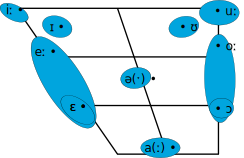
\includegraphics[width=.4\textwidth]{graphics/vowelcharts/pembrokeshire-stressed-penultima}}
  \subtop[Unstressed syllables before a consonant]{\includegraphics[width=.4\textwidth]{graphics/vowelcharts/pembrokeshire-unstressed-preconsonantal}}
  \subtop[Unstressed syllables before a vowel]{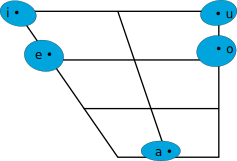
\includegraphics[width=.4\textwidth]{graphics/vowelcharts/pembrokeshire-unstressed-hiatus}}
  \subtop[Unstressed syllables word-finally]{\includegraphics[width=.4\textwidth]{graphics/vowelcharts/pembrokeshire-unstressed-word-final}}
  \caption{Vowels in Pembrokeshire Welsh}
  \label{fig:pw-vowels}
\end{figure}

\subsection{Diphthongs}
\label{sec:diphthongs-2}

Pembrokeshire Welsh has a relatively rich inventory of diphthongs, especially if we include sequences that look like rising diphthongs, such as \ipa{[we]}. However, it appears that the true phonological diphthongs (understood as tautosyllabic non\hyp onset vowels) are falling. I consider these first and then turn to the more problematic cases.

\subsubsection{Falling diphthongs}
\label{sec:falling-diphthongs}

In falling diphthongs, the non-syllabic element is either \ipa{[i]} or \ipa{[u]}. The quality of the nuclear element is for the most part identical to that of the corresponding monophthong, with the exception of \ipa{[ei]} and \ipa{[ou]}, where the nuclear vowel is higher than the monophthong (thus \phonint{e̝i~o̝u}), presumably due to some coarticulation from the following glide. All the diphthongs are shown in \cref{ex:pw-diphthongs}. As I discuss in \cref{sec:structure-diphthongs}, I analyse the offglides as featurally identical to high vowels, so in phonological transcription I will use the symbols \ipa{[i]} and \ipa{[u]} for the offglides.

\ex.\label{ex:pw-diphthongs}\a.\a.\fwe{ˈwein}{ˈwe̝i̯n}{gwaun}{moor}
\b.\fwe{ˈbraiχ}{brai̯x}{braich}{arm}
\b.\fwe{ˈtroi}{ˈtrɔi̯}{troi}{turn}
\b.\fwe{ˈhuir}{ˈhʊi̯r}{hwyr}{late}
\z.\b.\a.\fwe{ˈɬiu}{ˈɬɪu̯}{lliw}{colour}
\b.\fwe{ˈteu}{ˈtɛu̯}{tew}{fat}
\b.\fwe{ˈbraud}{ˈbrau̯d}{brawd}{brother}
\b.\fwe{ˈmour}{ˈmo̝u̯r}{mawr}{big}
\b.\fwe{ˈtəuiɬ}{ˈtəwˑiɬ}{tywyll}{dark}

As noted by \citet[p.~15]{awbery86:_pembr_welsh}, almost all diphthongs are \enquote{paired}, in the sense that both sets of diphthongs contain one diphthong with a high nucleus, one with a low nucleus, and two with mid nuclei (with the one in the same backness category as the glide being low-mid and the one in the same backness category being mid-high). Only \ipa{[əu]} is isolated in this respect, since there is no *\ipa{[əi]} in this dialect.\footnote{It seems that Standard Welsh \ipa{[əi]} (or \ipa{[əɨ]} in dialects which have \ipa{[ɨ]}; see \citealt[p.~727]{gyg}) often corresponds to Pembrokshire \phonint{e̝ĭ}.}

Phonetically, according to \citet[p.~16]{awbery86:_pembr_welsh}, the diphthongs are realized identically across most stress-related contexts: \blockquote{[t]he second element of the diphthong is [\ldots] predictably short in most contexts. This is true of [stressed] monosyllables, and of unstressed antepenultimates and finals.} In stressed penultimate syllables, however, the glide is said to be lengthened.

\ex.\a.\twp{ˈke̝jˑnɔɡ}{ceiniog}{penny}
\b.\twp{ˈe̝jˑra}{eira}{snow}
\b.\twp{ˈtəwˑiɬ}{tywyll}{dark}

\subsubsection{Gliding as phonetic readjustment}
\label{sec:gliding-as-phonetic}

At first blush, Pembrokeshire Welsh also possesses a rich inventory of what looks like rising diphthongs. However, in all of these cases the form with the glide is said to be in variation with one with a full vowel. One example of this variable gliding is found with unstressed high vowels before stressed vowels of penultimate syllables:

\ex.\label{ex:diwrnod-diawl}\a.\a.\twe{[duˈarnod]}{diwrnod}{day}
\b.\mbp{ˈdwarnod}
\z.\b.\a.\twe{[diˈaːvol]}{diawl}{devil}
\b.\mbp{ˈdjaːvol}

I suggest that in this case the variation is probably best described as phonetic. Given that high vowels are pronounced as tense allophones \phonint{i} and \phonint{u} before other vowels (as discussed in \cref{sec:unstressed-syllables}), the difference between a relatively short (in unstressed position) high vowel \phonint{i} (with a relatively narrow constriction) and a glide \phonint{j} is very small and possibly quantitative rather than qualitative. In other words, a short \phonint{i} or \phonint{u}, perhaps lacking a stable formant structure because of short duration, is easy to perceive as a glide rather than the nucleus of a syllable. Given that the conditions for the variation are not well described, I will take the conservative option and interpret it as non\hyp phonological: I will treat the forms in \cref{ex:diwrnod-diawl} as having surface\hyp phonological representations with three syllables: \ipa{[.di.ˈaː.vol.]}, \ipa{[.du.ˈar.nod.]}.

Once we accept that phonological surface vowels can be perceived as glides when they stand next to another, phonetically longer, vowel, we are in a position to understand the more puzzling type of gliding, which involves stressed vowels.

When a stressed high vowel stands in hiatus with a non-high vowel, there is an optional realization where the vowel is glided and the length is realized on the unstressed vowel. This happens irrespective of the presence of a morpheme boundary between the vowels: in \cref{bues}, the two vowels are separated by a morpheme boundary, whereas \cref{diod} is monomorphemic.

\ex.\a.\label{diod}\a.\twe{[ˈdiːod]}{diod}{drink}
\b.\mbp{ˈdjoːd}
\z.\b.\label{bues}\a.\twe{[ˈbiːes]}{bues}{(I) was}
\b.\mbp{ˈbjeːs}

Most surprisingly, this can lead to the creation of what is transcribed as a long vowel before a consonant sequence: a structure that is otherwise all but impossible in the language (\cref{sec:non-final-position}).\footnote{In addition, this type of lengthening may be out of line with the pattern of length specific to that particular morpheme (\cref{sec:contr-vowel-length}): \phonint{ˈfjoːl} `bowl' (\emph{ffiol}) despite plural \ipa{[ˈfjole]} (not *\ipa{[fjoːle]}).} In addition, the gliding seems to create complex onsets, which, as I discuss in \cref{sec:analysis-9}, are dispreferred in Pembrokeshire Welsh.

\ex.\a.\a.\twe{[ˈtuːarχ]}{tywarch}{peat}
\b.\mbp{ˈtwaːrχ}
\z.\b.\a.\twe{[ˈdiːolχ]}{diolch}{thanks}
\b.\mbp{ˈdjoːlχ}

I suggest that also in these cases there is no phonological alternation involved. The difference is due to a trade-off in phonetic length caused by the specifics of the phonetic implementation of stress. I propose that the surface\hyp phonological representation of a form like \phonint{ˈdjoːlχ} is still \ipa{[ˈdiːolχ]}; the transcription with an initial glide simply reflects the fact that the final unstressed vowel is phonetically longer than the stressed vowel. Given the phonetic similarity between tense high vowels \phonint{i~u}, which are the normal realization of stressed vowels in this position, and glides \phonint{w~j}, it is not at all surprising that a vowel can be pronounced and/or perceived as more glide-like in the neighbourhood of a phonetically longer vowel.

There are several reasons for the lengthening of the unstressed vowel. First, all relevant sequences consist of a high vowel followed by a non-high one (sequences of two high vowels are discussed in \cref{sec:flip-flop-altern}), and the greater inherent length of the latter might be a factor here. A second, probably more important, consideration involves the phonetic realization of stress and prominence. I discuss the distribution of length and its relationship to stress, as well as the phonological status of the relevant facts, in greater detail later (\cref{sec:real-stress-polysyll,sec:pros-prom-as}), but the basic idea is that, as shown by numerous investigations \citep{thomas67:_welsh,rhys84:_inton,williams85:_pitch_welsh,williams-eurospeech,williams99:_welsh,ball01:_welsh_phonet}, in certain prosodic contexts a phonologically unstressed final-syllable vowel can be phonetically long, to the point of being longer than the stressed vowel. Given this relationship, we could expect the phonetically shorter vowel of the penultimate syllable to be perceived as more of a glide.

The rôle of phonetic duration as a cue to prosodic structure in this pattern is underscored by the existence of examples such as the following:

\ex.\a.\label{ex:clywais}\a.\twe{[ˈkluːes]}{clywes}{(I) heard}
\b.\mbp{ˈklweːs}
\z.\b.\label{ex:clyw-clywed}\a.\twe{[ˈkləued]}{clywed}{to hear}
\b.\twe{[ˈkliu]}{clyw}{hearing}

The existence of forms such as those in \cref{ex:clyw-clywed} establishes beyond reasonable doubt that the underlying form of the stem \textsc{hear} is \ipa{/kləu/}; the expected 1st person past tense form of \cref{ex:clywais} is thus \ipa{[ˈkləues]} (\cf above \ipa{[ˈbiːes]} for the suffix). Similarly,  \ipa{[ˈtuːarχ]} `peat' is (at least historically) derived from \ipa{[ˈtəuarχ]}.\footnote{\citet[p.~154]{awbery86:_pembr_welsh} indeed records \ipa{[ˈtowarχ]} for `peat' in western varieties (where surface \ipa{[ə]} is dispreferred).} As mentioned in \cref{sec:falling-diphthongs}, the \enquote{glide} in such forms is pronounced long, and the phonetic distance between a \enquote{long glide} and a tense high vowel is not great. Once again, the timing in the recorded form such as \phonint{ˈklweːs} would appear to be an artefact of the phonetic distribution of length rather than of a phonological process. First, the supposed \enquote{glide} becomes more perceptually prominent than the stressed vowel (\phonint{ˈkl\textsuperscript{ə}uˑes} for phonological \ipa{[ˈkləues]}), but the glide itself can in turn be \enquote{hijacked} by the phonetic length of the following vowel, giving \phonint{ˈklweːs}.\footnote{The importance of the final syllable seems to be confirmed by \posscite{awbery86:_pembr_welsh} remark that \ipa{[i]} may be optionally pronounced as \phonint{ji} in a final unstressed syllable: \phonint{ˈmɛnjiw} or \phonint{mɛniw} for \ipa{[ˈmeniw]} `woman', \phonint{hɛðjiw} or \phonint{ˈheːðjiw} for \ipa{[ˈheːðiw]} `today'. It appears likely that the \phonint{ji} is also a product of phonetic lengthening, and the explicit association with the final unstressed syllable is suggestive.} Such \enquote{loss} of stressed vowels with retention of final ones has been extensively commented upon in the literature \citep{jones49:_moder_welsh,watkins76:_cyfnew_gymraeg,bosch96:_promin}, although usually treated from a diachronic standpoint or as a phonological process rather than as a matter of synchronic phonetic variation.

Further evidence for the phonetic nature of this \enquote{gliding} process is found in cases where the \enquote{glided} vowel is in fact mid. \citet{awbery86:_pembr_welsh} records variation of the following type:

\ex.\a.\a.\twe{[ˈdeːaɬ]}{deall}{understand}
\b.\mbp{ˈdiːaɬ}
\b.\mbp{ˈdjaːɬ}
\z.\b.\a.\twe{[ˈhiːol]}{heol}{farmyard}
\b.\mbp{ˈhjoːl}
\b.\mbp{ˈhewl}

There is no productive phonological process of raising that would explain the variation between \ipa{[e]} and \ipa{[i]} in these forms. However, if what is intended as a mid vowel is phonetically short enough compared to its neighbouring vocoid, it can be perceived as a glide (a front one in \phonint{ˈdjaːɬ} or, conversely, a back one in \phonint{hewl}). No appeal to variable, exception-creating phonology is needed: we only have to accept that the phonology\endash phonetics interface (or perhaps the postlexical phonology) in Pembrokeshire Welsh can severely disrupt the relative length (or in any case the perceptual prominence) of stressed and unstressed vowels.\footnote{Of course it is entirely possible that at least some speakers have begun to phonologize these patterns; however, discovering these patterns would require closely targeted empirical study, which I must leave for the future.}


\subsection{Consonants}
\label{sec:consonants}

The phonetic inventory of Pembrokeshire Welsh is shown in \cref{tab:pw-consonans}. Variants given with slashes indicate contextual allophony. I use the devoicing diacritic (as in \eg \phonint{ð̥}) to indicate that the relevant segment does not have consistent vocal fold vibration but retains other characteristics participating in the expression of the laryngeal contrast (\eg length, formant movements etc.).

\begin{table}[htp]
  \centering
\adjustbox{width=\textwidth}{  \begin{tabular}{l*{10}{>{\ipafont}l>{\ipafont}r}}
\toprule
Manner & \multicolumn{2}{c}{Bilabial} & \multicolumn{2}{c}{Labiodental} & \multicolumn{2}{c}{Dental} & \multicolumn{2}{c}{Alveolar} & \multicolumn{2}{c}{Postalveolar} & \multicolumn{2}{c}{Palatal} & \multicolumn{2}{c}{Velar}  & \multicolumn{2}{c}{Uvular} & \multicolumn{2}{c}{Glottal} \\
\midrule
Stops        & pʰ/p & b/b̥ &   &   &   &   & tʰ/t   & d/d̥   &     &      &   &  & kʰ/k & ɡ/ɡ̊ &   &  &    \\
Affricates   &   &   &   &   &   &   &     &     & (ʧʰ) & (dʒ/d̥ʒ̊) &   &  &   &   &   &  &    \\
Fricatives   &   &   & f & v/v̥ & θ & ð/ð̥ & s ɬ & (z/z̥) & ʃ   &      &   &  &   &   & χ &  & h  \\
Nasals       & m &   &   &   &   &   & n   &     &     &      &   &  & ŋ &   &   &  &    \\
Laterals     &   &   &   &   &   &   & l   &     &     &      &   &  &   &   &   &  &    \\
Rhotics      &   &   &   &   &   &   & r/r̥/ɾ/ɹ   &     &     &      &   &  &   &   &   &  &    \\
Approximants & w &   &   &   &   &   &     &     &     &      & j &  &   &   &   &  &    \\
\bottomrule
  \end{tabular}}
  \caption{Pembrokeshire Welsh consonants: the phonetic inventory}
  \label{tab:pw-consonans}
\end{table}

The contrast between \enquote{voiced} and \enquote{voiceless} stops is in reality one between variably voiced and aspirated stops: according to \citet[p.~13]{awbery86:_pembr_welsh}, \textquote{[v]oiceless stops are heavily aspirated in word-initial position, less so elsewhere}, while \textquote{[v]oiced stops and fricatives are fully voiced between vowels, partially voiced in other contexts.} This accords well both with non-instrumental descriptions of other Welsh varieties (\cf for instance \citealt{thomas61:_ffonem_dyffr_wysg,jones,brycheiniog}) and phonetic studies \citep{ball-phon,ball01:_welsh_phonet}.\footnote{A notable feature of the realization of laryngeal contrast in other Welsh varieties (and also in contact varieties of English, cf.\ \citealt{walters03:_celtic_englis}) is the existence of strong postaspiration in word-final and syllable-final position, which are more commonly associated with lack of release and phenomena such as glottalization in other languages. Note, however, that \citet{morris10:_phonet_north_wales} finds that some (Northern) Welsh speakers use variable (\ie \enquote{non\hyp normative} in \citeauthor{helgason}'s \citeyear{helgason} terms) preaspiration for coda stops.} As in many other languages making use of long-lag VOT stops, the laryngeal contrast is neutralized following the fricatives \ipa{[s]}, where stops are voiceless and unaspirated; see below \cref{sec:laryng-assim} for more discussion. The aspiration of stops manifests itself in partial devoicing of following sonorants:

\ex.\a.\twp{ˈpr̥ɛn}{pren}{tree}
\b.\twp{ˈpl̥\kern-1pt ant}{plant}{children}


The laryngeal contrast in fricatives in Welsh dialects is normally one of voicing (rather than VOT); however, as discussed \eg by \citet{ball01:_welsh_phonet}, \enquote{voiced} fricatives can in fact be partially devoiced in a manner similar to stops, although other cues such as duration remain. Since voiced fricatives are relatively rare in non\hyp voicing contexts (\eg word\hyp initially and word\hyp finally, see \cref{sec:phonotactics-1}), a full picture will have to emerge from targeted experimental study.

The rhotic \ipa{[r]} is normally a voiced tap or flap; word-initially, it may be devoiced, but the voiced and voiceless variants are said to be in free variation. Thus, Pembrokeshire Welsh lacks the contrast between \ipa{[r̥]} and \ipa{[r]}, which in other dialects is marginal word-initially but quite robust in non-initial position (however, \ipa{[rh]} sequences are apparently possible: see \cref{sec:story-ipah}).

\ex.\a.\twp{ˈr̥iːχ}{rhych}{furrow}
\b.\mbp{ˈriːχ}

Following alveolar stops, \ipa{[r]} is said to be realized as a fricative \phonint{ɹ}, as in \phonint{ˈdɹuːs} `door' (\emph{drws}).

The segment \ipa{[ŋ]} is found not only word-finally and before velar stops, but also word-medially before a vowel, as in \cref{ex:ng-pw}. It is not found word-initially.

\ex.\label{ex:ng-pw}\a.\twe{[ˈɬɔŋe]}{llongau}{ships}
\b.\twe{[kɪˈvɪŋi]}{cyfyngu}{confine}

The segments \ipa{[ʧ]}, \ipa{[dʒ]}, and \ipa{[z]} are only found in English borrowings, and I exclude them from further consideration here (round brackets in \cref{tab:pw-consonans}).

The inventory I will use in surface\hyp phonological transcriptions is given in \cref{tab:pw-consonants-phonological}. \begin{table}[tbp]
  \centering
\adjustbox{width=\textwidth}{\begin{tabular}{l*{10}{>{\ipafont}l>{\ipafont}r}}
\toprule
Manner & \multicolumn{2}{c}{Bilabial} & \multicolumn{2}{c}{Labiodental} & \multicolumn{2}{c}{Dental} & \multicolumn{2}{c}{Alveolar} & \multicolumn{2}{c}{Postalveolar} & \multicolumn{2}{c}{Palatal} & \multicolumn{2}{c}{Velar}  & \multicolumn{2}{c}{Uvular} & \multicolumn{2}{c}{Glottal} \\
\midrule
Stops        & p & b &   &   &   &   & t   & d   &     &      &   &  & k & ɡ &   &  &    \\
Affricates   &   &   &   &   &   &   &     &     & ʧ & dʒ &   &  &   &   &   &  &    \\
Fricatives   &   &   & f & v & θ & ð & s ɬ & z & ʃ   &      &   &  &   &   & χ &  & h  \\
Nasals       & m &   &   &   &   &   & n   &     &     &      &   &  & ŋ &   &   &  &    \\
Laterals     &   &   &   &   &   &   & l   &     &     &      &   &  &   &   &   &  &    \\
Rhotics      &   &   &   &   &   &   & r/r̥   &     &     &      &   &  &   &   &   &  &    \\
Approximants & w &   &   &   &   &   &     &     &     &      & j &  &   &   &   &  &    \\
\bottomrule
  \end{tabular}}
  \caption{Pembrokeshire Welsh consonants: the phonological inventory}
  \label{tab:pw-consonants-phonological}
\end{table} It is mostly isomorphic with the actual phonological representation, barring a few adaptations to the phonetic reality. The mapping between the surface\hyp phonological transcription used below and phonetics is made explicit in \cref{tab:transcription-pw}. \begin{table}[tbp]
  \centering
  \begin{tabular}{*{2}{>{\ipafont}l}p{.6\textwidth}}
    \toprule
    Phonology & Phonetics & Comments \\
    \midrule
    {[p t k]} & \phonint{p(ʰ) t(ʰ) k(ʰ)} & Aspirated in onsets, unaspirated voiceless (possibly short\hyp lag VOT) following other obstruents. See \cref{sec:laryng-assim} for motivation of the choice of \ipa{[p~t~k]} for the latter context \\
    {[b d ɡ]} & \phonint{b/b̥ d/d̥ ɡ/ɡ̊} & Consistently voiced in intersonorant context, less so elsewhere \\
    {[f θ χ s ʃ ɬ]} & \phonint{f θ χ s ʃ ɬ} & Voiceless, short\hyp lag VOT, relatively long with little contextual allophony \\
    {[v ð]} & \phonint{v/v̥ ð/ð̥}  & Consistently voiced in intersonorant context, less so elsewhere \\
    {[h]} & \phonint{h/ɦ/$\emptyset$} & Described as voiceless when word\hyp initial, sometimes deleted; presumably may be voiced in intersonorant contexts\\
    {[m n ŋ l]} & \phonint{m n ŋ l} & No significant contextual allophony described \\
    {[r/r̥]} & \phonint{r/r̥} & I write \ipa{[r̥]} word\hyp initially and \ipa{[r]} elsewhere despite the lack of phonological distinction to leave the transcription realistic \\
    {[u/w i/j]} & \phonint{w j} & I write \ipa{[u~i]} for monophthongs and off\hyp glides in diphthongs (\ie\ \ipa{[i~u]} that are tautosyllabic with a preceding vowel, even if the high vowel also forms an onset in the following syllable) and \ipa{[w~j]} for \enquote{pure} onsets\\
    \bottomrule
  \end{tabular}
  \caption{Transcription for Pembrokeshire Welsh}
  \label{tab:transcription-pw}
\end{table} In the remainder of this chapter, I will use the simplified transcription of \cref{tab:transcription-pw} for surface\hyp phonological representations, occasionally giving the phonetic forms for clarity.


\section{Prosodic structure and stress}
\label{sec:pros-struct-stress}

In this section I describe the word-level prosodic structure of Pembrokeshire Welsh, deferring discussion of syllable-related matters until \cref{sec:phonotactics-1}.

\subsection{Regular stress}
\label{sec:regular-stress}

As is normal in Welsh dialects otherwise, stress in Pembrokeshire Welsh falls within a two-syllable window at the right edge of the word. The normal situation is penultimate stress, irrespective of the \enquote{size} of the final syllable:

\ex.Final open syllable
\a.Penultimate open syllable
\a.\twe{[ˈboːre]}{bore}{morning}
\b.\twe{[ˈtɔri]}{torri}{to cut}
\z.\b.Penultimate closed syllable
\a.\twe{[ˈkadno]}{cadno}{fox}
\b.\twe{[ˈkɔpsi]}{copsi}{top of corn stack}

\ex.Final closed syllable
\a.Single final consonant
\a.\twe{[ˈskaːdan]}{sgadan}{herring}
\b.\twe{[ˈkrɪvder]}{cryfder}{strength}
\z.\b.Multiple final consonants
\a.\twe{[ˈmənwent]}{mynwent}{cemetery}
\b.\twe{[ˈaskurn]}{asgwrn}{bone}

\ex.Longer forms
\a.\twe{[kʊˈmʊsklid]}{cymysglyd}{muddled}
\b.\twe{[eˈboːles]}{eboles}{filly}
\b.\twe{[karˈθɛni]}{carthenni}{quilts}
\b.\twe{[posiˈbɪlrʊið]}{posibilrwydd}{possibility}
\b.\twe{[kineiˈaːvi]}{cynaeafu}{to harvest}
\b.\twe{[aniˈveiljed]}{anifeiliaid}{animals}

The stress all but never falls further from the right edge than the penultimate syllable, leading to alternations inside paradigms (see \cref{fn:exceptional-stress} below for a brief discussion of exceptions):

\ex.\label{ex:stress-movement}\a.\a.\twe{[ˈeːɡɪn]}{egin}{sprout}
\b.\twe{[ɛˈɡiːno]}{egino}{to sprout}
\z.\b.\a.\twe{[ˈɡɔːvɪn]}{gofyn}{ask}n
\b.\twe{[ɡɔˈvɪnoð]}{gofynnodd}{(s)he asked}

\subsection{Final stress}
\label{sec:final-stress}

In certain exceptional cases stress may fall on the final syllable. These are as follows.

\begin{itemize*}
\item English borrowings
\ex.\a.[]\twe{[sɪˈmɛnt]}{siment}{cement}\par
\item Lexical exceptions
\ex.\a.\twe{[maŋˈɡiː]}{mam-gu}{grandmother}
\b.\twe{[ɪwχˈbɛn]}{uwchben}{above}\par
\item Stems with prefixes (here exemplified by \emph{ail-} `re-')
\ex.\a.\twe{[ailˈhɔi]}{ailhau}{reseed}
\b.\twe{[ailˈneid]}{ailwneud}{redo}*\par
\item Diphthongs derived from vowel sequences straddling a morpheme boundary (synæresis):
\ex.\a.\twe{[ˈkəvle]}{cyfle}{chance}
\b.\twe{[kəvˈleis]}{cyfleus}{convenient}\par
Note that normally final-syllable diphthongs do not attract stress:
\ex.\a.[]\twe{[ˈdamwain]}{damwain}{accident}\par
\item Certain suffixes such as the verbalizing suffix \ipa{[ai]}:
\ex.\a.\twe{[ˈjaːχ]}{iach}{healthy}
\b.\twe{[jaˈχaːd]}{iachâd}{cure}
\b.\twe{[jaˈχai]}{iacháu}{to cure}\par
\end{itemize*}

\subsection{The realization of stress in polysyllables}
\label{sec:real-stress-polysyll}

I assume that the phonetic realization of stress in Pembrokeshire Welsh is not substantially different from that described for other varieties or for the language in general \citep{sommerfelt,jones49:_moder_welsh,pilch57:_lauts,watkins61:_ieith,thomas67:_welsh,rhys84:_inton,williams85:_pitch_welsh,williams99:_welsh,ball01:_welsh_phonet,bosch96:_promin,webb11:_welsh_englis}. Broadly speaking, the stressed (penultimate) syllable demonstrates certain durational properties, to which I return shortly, while final syllables (whether stressed or unstressed), in many prosodic contexts, host a rapid rise in pitch and a concomitant increase in duration \citep[\cfm][]{ohala78:_produc}. These durational and tonal characteristics of final syllables often conspire to give word\hyp final unstressed syllables greater perceptual prominence (at least in the ears of English speakers) than the preceding, stressed, syllable.\footnote{Many of the aspects of this system are also present in the prosodic system of Welsh English, both in the south \citep{walters03:_celtic_englis,walters03:_south_wales_valley_englis} and in the north \citep{webb11:_welsh_englis}.}

Despite this potential for greater salience of the final unstressed syllable, I follow the traditional description in identifying the penultimate syllable as stressed. This is because, as discussed above in \cref{sec:stress-headedness}, I take \enquote{stress} to refer to status as prosodic headship: stressed syllables should be the loci of phonological head\endash dependent asymmetries, and in \cref{sec:foot-intern-struct} I show that this is precisely the case for penultimate syllables in Welsh polysyllabic words.

As noted by \citet{jones67:_welsh,williams85:_pitch_welsh,williams99:_welsh,ball01:_welsh_phonet,webb11:_welsh_englis}, a very important phonetic cue of stress in Welsh is the lengthening of the consonant following a short stressed vowel in a penultimate syllable. It is indeed noted by \citet{awbery86:_pembr_welsh} for Pembrokeshire Welsh as well; she uses a \enquote{half-length} notation. This also covers the lengthening of the glide in a stressed diphthong described above (\cref{sec:diphthongs-2}).

\ex.\label{ex:penult-cons-lengthening}\a.\twp{ˈkarˑeɡ}{carreg}{stone}
\b.\twp{ˈamˑser}{amser}{time}
\b.\twp{ˈejˑra}{eira}{snow}

In \cref{sec:foot-intern-struct}, I analyse this lengthening as moraicity of the postvocalic consonant or glide, and identify the phonological nature of \enquote{stress} as bimoraicity. It would then be not surprising if the main phonetic correlate of stress had to do with highlighting this aspect of the structure of a word, and \citet{williams85:_pitch_welsh} does appear to reach a very similar conclusion: \blockquote[p.~382][.]{The only stress cues seem to be of a relational nature, concerning the relative timing of vowel and consonant, or the temporal arrangement of syllables into feet}

Although I believe this broad picture to be correct, there is an unresolved issue here requiring further study, which concerns the expression of stress in syllables with long vowels. Most previous work has concentrated on stressed syllables with short vowels. Part of the reason is that it is difficult to find minimal pairs with open penultimate syllables. As we saw in \cref{sec:final-stress}, unpredictable stress is rare, and the best chance of finding minimal pairs is connected with prefixes associated with monosyllabic stems, as in \posscite[']{williams85:_pitch_welsh} pair \emph{ymladd} \ipa{[ˈəmlað]} `fight'\,$\sim$\,\emph{ymlâdd} \ipa{[əmˈlaːð]} `tire oneself', and the lexicon of Welsh happens not to provide such forms where the penultimate stressed syllable would have a long vowel. Another aspect skewing the literature towards cases with a short vowel even in open syllables is the concentration on North Welsh: as briefly discussed above in \cref{sec:bryth-quant-syst} and exemplified below in \cref{sec:vowel-length}, in North Welsh \emph{all} stressed vowels in penultimate syllables are short, meaning that the pattern seen in \cref{ex:penult-cons-lengthening} is much more widespread than in South Welsh. The interaction of the hypothesis that it is relative duration within the head syllable that is the main phonetic correlate of stress and the vowel length contrast therefore remains understudied for now. I will return to this issue briefly below in \cref{sec:primacy-length}.

Another issue that would benefit from closer study is the status of the lengthening of the final unstressed syllables as phonetic or phonological. In the discussion of phonetic gliding in \cref{sec:gliding-as-phonetic} I assumed that this lengthening is not phonologized, and I transcribe words such as \ipa{[boːre]} `morning' and \ipa{[ˈkopsi]} `top of corn stack' with short vowels in final syllables rather than *\ipa{[ˈboːreː]} or \ipa{[ˈkopsiː]}. Ultimately, the reason for this is the conservative approach to phonological status I adopt by default: since I know of no phonological evidence that would compel us to include this lengthening in the phonology, and the phenomena that are related to this lengthening (pitch accent placement, phonetic gliding) are commonly described in the literature as \enquote{variable}, it seems safer to assume that it is not indeed phonological. It is of course possible that at least for some speakers this lengthening might have entered the postlexical phonology. Absent an interaction with other phonological processes, such an analysis would, however, at the very least require phonetic evidence for categorical distribution of length, which is not available to me at the moment.

I also discuss this issue below in \cref{sec:pros-prom-as}. In any case, even if the lengthening \emph{is} phonological, it would appear quite clear that it only enters the phonology at the postlexical level; the analysis of Pembrokeshire Welsh foot structure provided in \cref{sec:foot-intern-struct} is only intended to account for the output of the word level, meaning that the (non-)existence of final\hyp syllable lengthening in the postlexical phonology is irrelevant. Given all this, at present I consider it justified to retreat to the conservative position and treat the lengthening as a phonetic phenomenon rather than a categorical operation on prosodic structure.

\subsection{Antepenultimate deletion}
\label{sec:antep-delet}

\citet{awbery86:_pembr_welsh} does not describe any secondary stress for Pembrokeshire Welsh (and in general cites very few forms of at least four syllables). However, there is some evidence for foot structure (or rather lack thereof) in the phenomenon of antepenultimate deletion (\cf also \citealt{jones49:_moder_welsh,watkins76:_cyfnew_gymraeg,hannahs11:_welsh}).

Specifically, a vowel in an antepenultimate syllable (which is by necessity unstressed) that is also word-initial can be deleted, as long as the resulting form is in line with the phonotactic structure of the language:

\ex.\label{ex:pw-antepenult-deletion}\a.\a.\twe{[ˈɛskid]}{esgid}{shoe}
\b.\twe{[ˈskɪdje]}{esgidiau}{shoes}
\z.\b.\a.\twe{[ˈaːdar]}{adar}{birds}
\b.\twe{[ˈdɛːrin]}{aderyn}{bird}
\z.\b.\a.\twe{[ˈardal]}{ardal}{area}
\b.\twe{[arˈdaːloð]}{ardaloedd}{areas}
\b.*\mbi{[ˈrdaːloð]}

However, this phenomenon is not noted for longer forms:

\ex.\a.\twe{[aniˈveiljed]}{anifeiliaid}{animals}
\b.*\mbi{[niˈveiljed]}


\subsection{Consonant phonotactics, syllable structure, and vowel length}
\label{sec:phonotactics-1}

In this section I discuss the restrictions on syllable size and possible segment sequences identified by \citet{awbery86:_pembr_welsh}, as well as some phenomena related to sonority repairs. This will set the scene for the discussion of the central issue of vowel length, which is treated in \cref{sec:vowel-length}.

\subsubsection{Consonant sequences}
\label{sec:consonant-sequences-1}

The restrictions on word-initial and word-final clusters are relatively familiar, though I defer discussion of word-final restrictions until later.

\paragraph{Possible sequences}
\label{sec:possible-sequences}

Word-initially,  possible two-consonant sequences are obstruent\endash obstruent and obstruent\endash sonorant. In the former case, these are only \ipa{[sk~st~sp]} (where the stops are voiceless and unaspirated). As for obstruent\endash sonorant sequences, most combinations of manners are allowed, with the exception of fricatives before nasals:

\ex.\a.\twe{[ˈskaːdan]}{sgadan}{herring}
\b.\twe{[ˈklɪst]}{clust}{ear}
\b.\twe{[ˈkneɪ]}{cneu}{nuts}
\b.\twe{[ˈfrɔŋk]}{ffronc}{part of a pigsty}

\citet{awbery86:_pembr_welsh} does not discuss place restrictions in detail; in general in Welsh, there is a dispreference for coronal\endash coronal initial sequences, especially when the first segment is not a stop: \ipa{[sr]} in particular is impossible (not found in the corpus) and \ipa{[sl]} appears to be found mostly in loanwords, although it is not obvious that they are not nativized: \ipa{[sl]}\hyp initial words are well\hyp represented throughout Wales in \citet{thomas00:_welsh}. Similarly, the gap with \ipa{[sr]} could be just historical (given that historically initial *\emph{sr} changed to \emph{fr} while major sources of loanwords such as English also happen not to have \ipa{[sr]}\hyp initial words).

The standard language also allows the cross\hyp linguistically uncommon \ipa{[tl]} and \ipa{[dl]} as in \emph{tlawd} `poor' and \emph{tlws} `pretty': the latter word is unknown to Pembrokeshire informants for \citet{thomas00:_welsh}, and the former does have initial \ipa{[tl]} in the region (although initial \ipa{[kl]} is common in both of these words in other areas).

Three-consonant clusters word-initially are limited to two types. By far the most common is \ipa{[s]}\endash stop\endash sonorant (in principle \ipa{[r]} is most common as the final element):

\ex.\a.\twe{[ˈskraːveɬ]}{scrafell}{scraper}
\b.\twe{[ˈstrɔːdir]}{strodur}{cart saddle}

Another type is relatively unusual: in the sequences \ipa{[ɡwl]} and \ipa{[ɡwr]} the \ipa{[w]}, contrary to expectations (see below \cref{sec:analysis-9}), remains non\hyp syllabic, even though the alternative forms with a vowel are in principle unobjectionable from a phonotactic perspective.

\ex.\a.\label{ex:gwlan-gwrug}\a.\twe{[ˈɡwlaːn]}{gwlan}{wool}
\b.\twe{[ˈɡwriːɡ]}{gwrug}{heather}
\z.\b.\a.*\mbi{[ˈɡuːlan]}
\b.*\mbi{[ˈɡuːriɡ]}

As discussed below in \cref{sec:analysis-9}, the behaviour of \ipa{[ɡw]} sequences in Pembrokeshire Welsh is special in other aspects too. However, I leave a full analysis of forms such as those in \cref{ex:gwlan-gwrug} for further work, since it is not entirely clear to me how \ipa{[ɡwl]} and \ipa{[ɡwr]} sequences are realized (for instance, it would be interesting to know to what extent the labialization gesture overlaps with the following sonorant).

The set of word-medial consonant sequences includes both sequences that are allowed word-initially and a number of others that are best treated as being broken up by a syllable boundary. These latter include sequences which consist of licit codas followed by single onsets, including sonorant\endash obstruent and sonorant\endash sonorant sequences which are impossible word-initially, as seen in \cref{ex:pw-medial-seqs}.

\ex.\label{ex:pw-medial-seqs}\a.\twe{[ˈɡʊmpas]}{o gwmpas}{around}
\b.\twe{[ˈkɛrðɛd]}{cerdded}{to walk}
\b.\twe{[ˈdaχre]}{dechrau}{begin}
\b.\twe{[ˈamlʊɡ]}{amlwg}{obvious}
\b.\twe{[ˈhɛdvan]}{hedfan}{to fly}

Word-medial sequences of three consonants can, for the most part, be analysed as sequences of a licit coda and a licit complex onset; \citet[p.~109]{awbery86:_pembr_welsh} lists some additional restrictions (for instance, only liquids are allowed as third elements in such sequences), but it is not clear to what extent these are principled. Examples are given in \ref{ex:pw-complex-seqs}.

\ex.\label{ex:pw-complex-seqs}\a.\twe{[ˈəsprid]}{ysbryd}{ghost}
\b.\twe{[ˈkɪndron]}{cynrhon}{maggots}
\b.\twe{[ˈmɔχtra]}{mochdra}{filth}

There are some alternations which appear to enforce the above generalization, in that an expected three\hyp consonant sequence that cannot be parsed as consisting of a simple coda and a licit branching onset is simplified (for the second vowel of \cref{ex:dwfn}, see below \cref{sec:rising-sonority}):

\ex.\a.\label{ex:dwfn}\twe{[ˈduːvun]}{dwfn}{deep}
\b.\twe{[ˈdʊnder]}{dyfnder}{depth}
\b.*\mbi{[ˈdʊvnder]}

However, there are a few examples that cannot be explained in this way.

\ex.\a.\label{ex:ieuanc}\a.\twe{[ˈiːvaŋk]}{ifanc}{young}
\b.\label{ex:ieuenctid}\twe{[ˈjɛŋktid]}{ieuenctid}{youth}
\z.\b.\label{ex:pw-parsley}\a.[]\twe{[ˈparsli]}{}{parsley}

Example \ref{ex:pw-parsley} is clearly a borrowing (and recall that \ipa{[sl]} appears to be allowed even if rare in the native lexicon). In \ref{ex:ieuenctid} the offending sequence is broken up by a morpheme boundary at least historically, though given the non-transparent relationship between the forms in \ref{ex:ieuanc} it cannot be taken for granted that \ref{ex:ieuenctid} is synchronically analysable as a complex word.

Finally, if the glides in diphthongs are treated as consonants, there is at least one example of a tri\hyp consonantal sequence involving a glide as the first element and not interpretable as containing an allowed complex onset:

\ex.\a.\twe{[ˈneiɬti]}{neilltu}{apart}
\b.\twe{[neiɬˈtiːol]}{neilltuol}{special}\footnote{The actual form as recorded by \citet{awbery86:_pembr_welsh} is \phonint{neiɬˈtjoːl}, but see \cref{sec:gliding-as-phonetic}.}

\paragraph{Distributional restrictions}
\label{sec:distr-restr}

There are two important restrictions on consonant sequences that are sometimes enforced by alternations.

First, nasals preceding a stop are almost always homorganic with that stop:

\ex.\a.\twe{[ˈpɪmp]}{pump}{five}
\b.\twe{[ˈmɛntiɡ]}{benthyg}{lend}
\b.\twe{[ˈwɪŋki]}{gwenci}{weasel}

This appears to be enforced in alternations, although given the paucity of stop\hyp initial suffixes the examples mostly come from compounding, raising morphological questions (note also the irregular stress in \cref{ex:mam-gu}).

\ex.\a.\a.\twe{[ˈɬiːn]}{Llun}{Monday}
\b.\twe{[ˈɬɪŋɡwin]}{Llungwyn}{Whit Monday}
\z.\b.\a.\twe{[ˈmam]}{mam}{mother}
\b.\label{ex:mam-gu}\twe{[maŋˈɡiː]}{mamgu}{grandmother}

The exceptions are said to be \enquote{very few}, but are found:\footnote{There are many more examples in the corpus, such as \emph{damcaniaeth} `theory', \emph{canpunt} `hundred pounds', \emph{rhanbarth} `region', although it is not known how these are pronounced in the dialect}

\ex.\a.\twe{[ˈamkan]}{amcan}{idea}
\b.\twe{[ˈprɪŋder]}{prinder}{scarcity}\footnote{Given that the root for `scarce' is undoubtedly \ipa{/prin/} in the dialect (\ipa{[ˈprɪn]} `scarce', \ipa{[ˈprɪnaχ]} `scarcer'), the form written \ipa{[ˈprɪŋder]} might represent the over-analysed transcription of a phonetic \phonint{ˈprɪɪ̃der}, where a surface-phonological \ipa{[n]} manifests itself simply as nasalization but is interpreted as a velar nasal \citep[\cfm][]{trigo88}.}

Fricatives do not enforce this requirement (no examples for the non-coronal fricatives \ipa{[f]} and \ipa{[v]}):

\ex.\a.\twe{[ˈhamðen]}{hamdden}{leisure}
\b.\twe{[ˈpʊmθeɡ]}{pymtheg}{fifteen}

Heterorganic sonorant sequences are also allowed:

\ex.\a.\twe{[ˈamluɡ]}{amlwg}{obvious}
\b.\twe{[ˈkʊmni]}{cwmni}{company}

Another restriction concerns laryngeal features: according to \posscite{awbery86:_pembr_welsh} formulation, clusters of two obstruents always agree in voicing. This is largely true in terms of static distribution:

\ex.\a.Voiced obstruent sequences
\a.\twe{[ˈɡʊðɡe]}{gyddfau}{necks}
\b.\twe{[əsˈtɛðvod]}{eisteddfod}{Welsh cultural festival}
\z.\b.Voiceless obstruent sequences
\a.\twe{[ˈkɔpsi]}{copsi}{top of corn stack}
\b.\twe{[ˈpɪstiɬ]}{pistill}{spring}

However, disharmonic sequences of two fricatives appear to be possible: \ipa{[ˈseiθved]} `seventh' (\emph{seithfed}) \ipa{[ˈʊiθved]} `eighth' (\emph{wythfed}) are recorded for all relevant locations in \citet[\emph{sub vocibus}]{thomas00:_welsh}.\footnote{Such sequences are relatively rare in Welsh vocabulary, but lexicographical sources for other dialects seem to confirm that there is no assimilation in these cases, \eg in Nantgarw \citep{thomas93:_tafod_nantg}: \ipa{[aˈrosva]} `sheep fold' (\emph{arhosfa}), \ipa{[ɡorˈfʊisva]} `resting place' (\emph{gorffwysfa}).}

Alternations enforcing this restriction are discussed in \cref{sec:laryng-assim}.

\subsubsection{Word-final phonotactics}
\label{sec:word-final-phon}

There are two aspects of word-final phonotactics that merit discussion here: relaxed restrictions on syllable size and sonority-related repairs.

\paragraph{Syllable size}
\label{sec:syllable-size}

As discussed in \cref{sec:possible-sequences}, most consonant sequences in Pembrokeshire Welsh can be analysed as being broken up by a syllable boundary after the first consonant, meaning that the coda of the syllable is almost always simple. This restriction is relaxed in word-final position, though the possible sequences are all of non-rising sonority (if sonority is defined according to standard assumptions).

\ex.\label{ex:complex-codas}\a.\twe{[ˈɡarð]}{gardd}{garden}
\b.\twe{[ˈklɪst]}{clust}{ear}
\b.\twe{[ˈɡwaɬt]}{gwallt}{hair}
\b.\twe{[ˈdarn]}{darn}{piece}

Such \enquote{complex codas} are also possible in polysyllabic forms, where they are not immediately preceded by a stressed vowel:

\ex.\a.\twe{[ˈfeːnest]}{ffenestr}{window}
\b.\twe{[ˈmənwent]}{mynwent}{cemetery}
\b.\twe{[ˈaskurn]}{asgwrn}{bone}

\citet[pp.~87--94]{wmffre03:_languag_wales} describes the simplification of final consonant sequences in polysyllabic forms as fairly widespread in his Ceredigion material. It would appear that the Pembrokeshire dialects are more conservative in this regard (for instance, they preserve the final sequence in \emph{asgwrn}, which \citeauthor{wmffre03:_languag_wales} \cite*{wmffre03:_languag_wales} singles out as prone to reduction). However, isolated examples of such \enquote{optional} simplification are also found in Pembrokeshire, apparently with alternations (for the \alternation{[u]}{[ə]} alternation, see below \cref{sec:vowel-mutation}):

\ex.\a.\a.\twe{[ˈsaːdurn]}{Sadwrn}{Saturday}
\b.\mbi{[ˈsaːdun]}
\z.\b.\a.[]\twe{[saˈdərne]}{Sadyrnau}{Saturdays}*

\citet{awbery86:_pembr_welsh} does not describe the precise nature of this variation, so I ignore the possibility of this simplification below.

In addition, a word-final consonant sequence may also be preceded by the glide element of a diphthong:\footnote{The forms appear to contain diphthongs rather than bisyllabic sequences with hiatus. If the latter were the case, we would expect the first vowel to be long, \cf bisyllabic \ipa{[ˈdeːaɬ]} `understand'.}

\ex.\a.\twe{[ˈmaint]}{maint}{size}
\b.\twe{[ˈbeirð]}{beirdd}{poets}*

\paragraph{Rising sonority}
\label{sec:rising-sonority}

Final consonant sequences of rising sonority (or, to be more precise, sequences consisting of an obstruent and a sonorant) are impossible in Pembrokeshire Welsh. Such sequences are found morpheme-finally, but when such morphemes are found word-finally, the offending sequence can be repaired in several ways. \citep{welshphonotactics,awbery86:_pembr_welsh,hannahs09:_welsh}. In Pembrokeshire Welsh, the attested repairs are epenthesis, deletion, and gliding, distributed as follows.

\subparagraph{Epenthesis}
\label{sec:epenthesis}

In the most common case, a vowel is epenthesized between the two final consonants. In terms of (phonological) quality, it is always a copy of the closest vocalic segment to the left, \ie of the stressed monophthong or of the glide part of a diphthong:\footnote{That the alternation represents epenthesis and not vowel deletion is confirmed by the existence of non-alternating vowels, as in \ipa{[ˈmuːdul]}\,$\sim$\,\ipa{[muˈduːle]} `haycock (sg.\,$\sim$\,pl.)'; the form *\ipa{[ˈmʊdle]} is phonotactically acceptable.}

\ex.\a.\a.\twe{[ˈɬɛster]}{llestr}{dish}
\b.\twe{[ˈɬɛstri]}{llestri}{dishes}
\z.\b.\a.\twe{[ˈsoudul]}{sawdl}{heel}
\b.\twe{[ˈsoudle]}{sawdlau}{heels}

The alternation seems to be driven by sonority rather than the identity of the consonants as an obstruent or a sonorant, since epenthesis also applies in all-sonorant sequences:

\ex.\a.\twe{[ˈamal]}{aml}{often}
\b.\twe{[ˈamlaχ]}{amlach}{more often}

However, there are occasional instances (apparently lexically determined) where a similar phenomenon applies in a context that cannot be described in terms of rising sonority:

\ex.\a.\a.\twe{[ˈheːlem]}{helm}{corn stack}
\b.\twe{[ˈhɛlmi]}{helmi}{corn stacks}
\z.\b.\label{ex:pw-gwddf}\a.\twe{[ˈɡuːðuɡ]}{gwddf}{neck}
\b.\twe{[ˈɡʊðɡe]}{gyddfau}{necks}

It appears difficult to extract any generalizations as to what besides rising sonority motivates the epenthesis. No other examples are recorded by \citet{awbery86:_pembr_welsh}. In the literary language, both \ipa{[ðɡ]} and \ipa{[lm]} are allowed, although rare in this position for historical reasons (but \cf \emph{ffilm} `film', \emph{balm} `balm', \emph{salm} `psalm'). For the similar sequence \ipa{[rm]}, \citet[\emph{sub voce}]{thomas00:_welsh} records \ipa{[ˈstoːrom]} for \emph{storm} `storm' but \ipa{[ˈfarm]} for \emph{fferm} `farm'. The latter could be a borrowing, although its short vowel contrasts with a long one in the clearly non\hyp nativized \ipa{[ˈɡaːrd]} `(fire) guard'. \citet[§4.13]{schumacher11:_mittel_fruhn} notes that in Middle Welsh epenthesis into the sequences \ipa{[lv]}, \ipa{[rv]}, \ipa{[lm]}, \ipa{[rm]} and \ipa{[ðv]} (the latter being historically present in words such as \ipa{[ˈɡuːðuɡ]}) was regular: Middle Welsh \emph{palyf} `palm', \emph{furyf} `form'. However, it seems than not all modern dialects retain this: Nantgarw \ipa{[ˈpalv]} `paw' \citep[\emph{sub voce}]{thomas93:_tafod_nantg}, Pembrokeshire \ipa{[ˈfirv]} `form' \citep[p.~71]{awbery86:_pembr_welsh}.

As discussed by \citet{hannahs09:_welsh}, despite the fact that the vowel is a copy of the preceding vocoid, it is apparently not an intrusive vowel \citep{levin87:_between,hall-intrusion} similar to that found in Scottish Gaelic, which has been analysed, at least for some dialects, as being an extension of the vocalic gesture \citep{hind-epenthesis,bosch-dejong,hall-intrusion} rather than the result of a phonological operation such as copying \citep{clements-barra,smith-gaelic,nevins10:_local}. In particular, as seen in examples such as \ref{ex:pw-gwddf}, the epenthetic vowel in Pembrokeshire Welsh is visible for the purpose of prosodic structure, since it behaves in line with the restrictions on the distribution of long vowels operative in the language otherwise (see \cref{sec:vowel-length} for details). I will therefore assume that the two vowels are indeed nuclei of two different syllables.

\subparagraph{Deletion}
\label{sec:deletion}

When the potential form with epenthesis would normally be parsed with three vocalic nuclei, epenthesis is blocked and deletion is deployed instead:

\ex.\label{ex:pw-sonority-driven-deletion}\a.\a.\twe{[feˈnɛstri]}{ffenestri}{windows}
\b.\twe{[ˈfeːnest]}{ffenestr}{window}
\b.*\mbi{[ˈfeːnestr]}
\b.*\mbi{[feˈnɛster]}
\z.\b.\a.\twe{[aˈnadli]}{anadlu}{breathe}
\b.\twe{[ˈaːnal]}{anadl}{breath}

As \cref{ex:pw-sonority-driven-deletion} shows, either the final sonorant or the obstruent preceding it may undergo deletion. According to \citet{awbery86:_pembr_welsh}, there is no clear pattern that would predict which process applies in each particular case, although \citet[ch.~22]{wmffre03:_languag_wales} claims that the sequence \ipa{[dl]} prefers deletion of the stop and other sequences normally prefer sonorant deletion; see also \citet{russell84:_welsh,schrijver95:_studies_britis_celtic,thomas95:_un_fryth}.

\subparagraph{The case of [v]}
\label{sec:case-ipav}

Finally, the behaviour of sequences starting with \ipa{[v]} is less predictable. In some cases, they undergo regular epenethesis.

\ex.\a.\a.\twe{[ˈtreːven]}{trefn}{order}
\b.\twe{[ˈtrɛvni]}{trefnu}{arrange}
\z.\b.\a.\twe{[ˈoːvon]}{ofn}{fear}
\b.\twe{[ˈɔvni]}{ofni}{to fear}

In other cases, the \ipa{[v]} is (variably) realized as a glide \ipa{[w]}; the resulting sequences are, according to \citet[p.~95]{awbery86:_pembr_welsh}, indistinguishable from \ipa{[ʊ]}-final diphthongs (though this has not been verified experimentally):

\ex.\label{ex:cefn-sofl-ysgafn}\a.\twe{[ˈkɛun]}{cefn}{back}
\b.\twe{[ˈsoul]}{sofl}{stubble}
\b.\twe{[ˈəskaun]}{ysgafn}{light}

However, this gliding is probably not a strategy for repairing sonority violations: in these particular forms the gliding of the \ipa{[v]} applies also in non-final syllables, where it cannot be motivated by sonority.

\ex.\a.\twe{[ˈkɛune]}{cefnau}{backs}
\b.\twe{[əsˈkaunaχ]}{ysgafnach}{lighter}

It would seem that the forms in \cref{ex:cefn-sofl-ysgafn} simply represent new underlying forms with diphthongs rather than \ipa{[v]}\endash sonorant sequences. That this is a lexical phenomenon is confirmed by the coexistence of different underlying representations (as in \ipa{[ˈkowru]} or \ipa{[ˈkəvru]} for \emph{cyfrwy} `saddle'), and by the fact that there are differences among dialects as to which lexical items allow which variants, indicating that the new forms are spreading by lexical diffusion. I will therefore ignore this behaviour of \ipa{[v]} in the formal account.

Remarkably, \citet{awbery86:_pembr_welsh} claims that in polysyllabic forms with \ipa{[v]} (\ie for those speakers who have not changed the representation of the lexical item to contain a diphthong) the entire sequence is retained:\footnote{This might be a peculiarity of the sequence \ipa{[vn]}: as noted by \citet{hannahs09:_welsh}, this sequence is more regularly allowed word-finally in Northern Welsh \citep[\egm][\emph{s.\,vv.\@} \emph{cefn}, \emph{cafn}, \emph{ofn}, \emph{dwfn}]{thomas00:_welsh}, as are other \ipa{[v]}\endash sonorant sequences (\emph{gafr}, \emph{llyfr}, \emph{llyfn}). The special status of \ipa{[v]} with respect to rising\hyp sonority consonant sequences in Brythonic languages is also discussed below in \cref{sec:asid-prov-leon}.}

\ex.\a.\twe{[ˈəskavn]}{ysgafn}{light}
\b.*\mbi{[ˈəskav]}
\b.*\mbi{[ˈəskan]}

\subsubsection{Restrictions on single consonants}
\label{sec:restr-single-cons}

Most single consonants may appear in most positions in the word. However, there are some restrictions that are also enforced by alternations.

\paragraph{Initial consonants}
\label{sec:initial-consonants}

Some consonants never appear in initial position. These are \ipa{[ð]} (where \ipa{[v]} is acceptable), \ipa{[θ]}, \ipa{[χ]}, and \ipa{[ŋ]}. Note than all of these are possible in the context of mutation: \ipa{[ð]} is the soft mutation of \ipa{[d]}, \ipa{[θ]} and \ipa{[χ]} are the spirant mutation correspondents of \ipa{[t]} and \ipa{[k]}, and \ipa{[ŋ]} is the nasal mutation of \ipa{[ɡ]}.

At first blush, one could assume that the lack of these segments word\hyp initially is a historical accident. Specifically, voiced fricatives only go back to postvocalic stops, meaning they are almost never found in initial position outside mutation contexts: the few instances found in Modern Welsh are either the result of context-free mutation, as in \emph{fel} `as, how', Middle Welsh \emph{mal}, \emph{ual}, or the dropping of an initial vowel, as in \emph{felly} `so', Middle Welsh \emph{yuelly} \citep{wg-mj,simonevans}. Similarly, \ipa{[θ]} and \ipa{[χ]} go back to geminates (or arise in positions following other segments, \eg liquids, being by necessity non\hyp initial) and \ipa{[ŋ]} could only appear before \ipa{[ɡ]}. All these structures were impossible in initial position at earlier stages of the language.

However, as discussed by \citet{awbery86:_pembr_welsh}, these restrictions are also enforced by the phonology, in that antepenultimate deletion (\cref{sec:antep-delet}) is disallowed if the resulting form were to begin with one of these consonants:

\ex.\a.\twe{[ˈiːχel]}{uchel}{high}
\b.\twe{[iˈχeːlaχ]}{uwch}{higher}
\b.*\mbi{[ˈχeːlaχ]}

\paragraph{Final consonants}
\label{sec:final-consonants}

Most consonants can be found in final position (though \ipa{[h]} is apparently excluded). However, the voiced fricatives \ipa{[v]} and \ipa{[ð]} have a less stable status, in that in certain lexical items they are deleted in this position:

\ex.\a.\a.\twe{[ˈklau]}{clawdd}{hedge}
\b.\twe{[ˈklɔðje]}{cloddiau}{hedges}
\z.\b.\a.\twe{[ˈtreː]}{tref}{town}
\b.\twe{[ˈtreːvið]}{trefoedd}{towns}

However, in other lexical items they remain stable:

\ex.\a.\a.\twe{[ˈkriːv]}{cryf}{strong}
\b.\twe{[ˈkriːvaχ]}{cryfach}{stronger}
\z.\b.\a.\twe{[ˈbeːð]}{bedd}{grave}
\b.\twe{[ˈbeːðe]}{beddau}{graves}

The distinction seems to be purely lexical: \blockquote[\citealt{awbery86:_pembr_welsh}, p.~100]{The choice of which items drop the \ipa{[v]} and \ipa{[ð]} and which keep them is very consistent throughout the area. There are no indications of geographical variation, with one district taking the trend further than another}. This is consistent with data from \citet{thomas00:_welsh}, where deletion of final \ipa{[ð]} and \ipa{[v]} is clearly restricted lexically: it completely fails in some words and varies geographically in others. For instance, \ipa{[ˈpriːð]} `soil', \ipa{[ˈkriːð]} `cobbler', and \ipa{[ˈprauv]} `test' appear with final fricatives throughout Wales,\footnote{Where the word is known: for instance, knowledge of the word \ipa{[ˈprauv]} was denied by the Pencaer informants.} while \emph{cryf} `strong' appears as \ipa{[krɨː]} in most of North Wales but \ipa{[ˈkriːv]} in the south. Conversely, \emph{clawdd} is realized as \ipa{[ˈklauð]} in most localities, with \ipa{[ˈklau]} clearly a south-western form.

Both laryngeal classes of final stops, on the other hand, are found word-finally:

\ex.\a.\a.\twe{[ˈhaːd]}{had}{seed}
\b.\twe{[ˈkrʊt]}{crwt}{boy}
\z.\b.\a.\twe{[ˈsɛld]}{seld}{dresser}
\b.\twe{[ˈsʊɬt]}{swllt}{shilling}
\z.\b.\a.\twe{[ˈkɪndruɡ]}{cynddrwg}{as bad}
\b.\twe{[ˈɬɔk]}{lloc}{sheepfold}

\paragraph{Restrictions on \ipa{/h/}}
\label{sec:restrictions-ih}

The segment \ipa{[h]} falls under a number of additional restrictions. Most importantly, it only appears initially and immediately before a stressed vowel (in which latter case it may only be preceded by a vowel or a nasal). This leads to alternations such as the following:\footnote{Unfortunately \citet{awbery86:_pembr_welsh} gives no examples of a similar alternation following a vowel. In the standard language, the alternation is found not only following nasals but also with \ipa{[r̥]}, as in \emph{arhosaf} `(I) will wait'\,$\sim$\,\emph{aros} `to wait', but \ipa{[r̥]} is absent from the inventory in Pembrokeshire Welsh, although \ipa{[rh]} sequences are recorded in \citet{thomas00:_welsh}; see further \cref{sec:story-ipah}. Following vowels, the standard language mostly prescribes retention of \ipa{[h]} in all contexts, as in \emph{cyhoeddi} `announce'\,$\sim$\,\emph{cyhoedd} `public' (but \emph{ar goedd} `common knowledge'), though a few items follow the restriction on \ipa{[h]}: \emph{ehangu} `widen'\,$\sim$\,\emph{eang} `wide' \citep[§II.53]{gyg}.}

\ex.\a.\a.\twe{[kənˈheia]}{cynhaeaf}{harvest}
\b.\twe{[kəneiˈaːvi]}{cynaeafu}{to harvest}
\z.\b.\a.\twe{[brenˈhiːnes]}{brenhines}{queen}
\b.\twe{[ˈbrɛnin]}{brenin}{king}

In addition, an onset \ipa{[h]} does not prevent antepenultimate deletion (\cref{sec:antep-delet}), even though technically the resulting sequence would be phonotactically impossible:

\ex.\a.\twe{[ˈhɔsan]}{hosan}{sock}
\b.\twe{[ˈsaːne]}{hosanau}{socks}
\b.*\mbi{[ˈhsaːne]}

In \cref{sec:story-ipah} I offer an analysis of the distribution of \ipa{[h]} as a deletion\dash or rather a selective preservation\dash process, building on work by \citet{hannahs11:_welsh}.

Finally, the segment \ipa{[h]} can in fact be freely deleted from all contexts, though the nature of the variation is not described in detail by \citet{awbery86:_pembr_welsh}:

\ex.\a.\a.\twe{[kənˈheia]}{cynhaeaf}{harvest}
\b.\mbi{[kəˈneia]}
\z.\b.\a.\twe{[ˈheːn]}{hen}{old}
\b.\mbi{[ˈeːn]}

Given the lack of data, I ignore this variability in the analysis that follows.

Phonotactic restrictions on consonants other than \ipa{[h]} are summarized in \cref{tab:pw-phonotactic-restrictions}. The question marks refer to cases where I have not been able to locate a dialect form (although the written language may have some of the relevant sequences; see \cref{sec:data-5} below for more discussion).

\begin{sidewaystable}
  \centering
  \begin{tabular}{>{\ipafont}l*{7}{>{\ipafont}c}}
    \toprule
          &                  & \multicolumn{4}{c}{Adjacent segment} &                                                                               \\
    \cmidrule{3-6}
    Class & Word-initial     & Voiced stop                          & Voiceless stop & Voiced fricative & Voiceless fricative & Word-final          \\
    \midrule
    p t k & \checkmark       & \delmark                             & \checkmark     & ?                & \checkmark          & \checkmark          \\
    b d ɡ & \checkmark       & \delmark                             & \delmark       & \checkmark       & \delmark            & \checkmark          \\
    v ð   & \scm v *ð        & \checkmark                           & ?              & \checkmark       & \checkmark          & \delmark/\checkmark \\
    f θ χ & \scm f *θ *χ     & \delmark                             & \checkmark     & \checkmark       & ?                   & \checkmark          \\
    s ʃ ɬ & \checkmark       & \delmark                             & \checkmark     & ?                & ?                   & \checkmark          \\
    m n ŋ & \scm m \scm n *ŋ & \checkmark                           & \checkmark     & \checkmark       & \checkmark          & \checkmark          \\
    l r   & \checkmark       & \checkmark                           & \checkmark     & \checkmark       & \checkmark          & \checkmark          \\
    \bottomrule
  \end{tabular}
  \caption{Phonotactic restrictions on consonants in Pembrokeshire Welsh}
  \label{tab:pw-phonotactic-restrictions}
\end{sidewaystable}

\subsubsection{Vowel length}
\label{sec:vowel-length}

The issue of the predictability of vowel (or rather monophthong) length is central to the prosody of the Brythonic languages, and Pembrokeshire Welsh is no exception in this regard. In this section I provide a description of the distributional facts, with the analysis to follow below in \cref{sec:foot-intern-struct} in the context of well-defined phonological representations.

As discussed by \citet{welshphonotactics,awbery86:_pembr_welsh}, the length of stressed vowels (whether in penultimate or final syllables) in Welsh is tightly connected to the nature of the consonant following the vowel. The relationship is particularly involved in southern dialects (including Pembrokeshire Welsh), where the vowel length contrast is found in both final and penultimate syllables; in northern dialects, the contrast is always neutralized in stressed penultimate syllables in favour of the short vowel:

\ex.South Welsh
\a.Final stressed syllables (overwhelmingly monosyllables)
\a.\twe{[ˈdiːn]}{dyn}{man}
\b.\twe{[ˈɡwɪn]}{gwyn}{white}
\z.\b.Penultimate stressed syllables
\a.\twe{[ˈaːraɬ]}{arall}{other}
\b.\twe{[ˈkareɡ]}{carreg}{stone}

\ex.\label{ex:northwelsh-vowel-length}North Welsh
\a.Final stressed syllables (overwhelmingly monosyllables)
\a.\twe{[ˈdɨːn]}{dyn}{man}
\b.\twe{[ˈɡwɨn]}{gwyn}{white}
\z.\b.Penultimate stressed syllables
\a.\twe{[ˈaraɬ]}{arall}{other}
\b.\twe{[ˈkaraɡ]}{carreg}{stone}

Since the restrictions on vowel length in stressed penultima and final stressed syllables are rather similar in Pembrokeshire Welsh, in what follows I treat them together. I also give the forms in both phonological and highly detailed phonetic transcription. Vowel quality is irrelevant, with the exception of \ipa{[ə]}, on which see \cref{sec:central-vowel}.

\paragraph{Contrastive vowel length}
\label{sec:contr-vowel-length}

Vowel length is contrastive in stressed syllables before the segments \ipa{[n]}, \ipa{[l]}, and \ipa{[r]}, \ie both long and short vowels are encountered before these consonants, with a lexical distribution. (Recall that I ignore the lengthening of final syllables discussed in \cref{sec:real-stress-polysyll}.)

\ex.Monosyllables
\a.The nasal \ipa{[n]}
\a.\fwe{ˈsuːn}{ˈsuːn}{sŵn}{noise}
\b.\fwe{ˈɡrʊn}{ˈɡrʊn}{grwn}{ridge of ploughland}
\z.\b.The lateral \ipa{[l]}
\a.\fwe{ˈsiːl}{ˈsiːl}{Sul}{Sunday}
\b.\label{ex:pw-wal}\fwe{ˈwal}{ˈwal}{wal}{wall}
\z.\b.The rhotic \ipa{[r]}
\a.\fwe{ˈtiːr}{ˈtʰiːr}{tir}{land}
\b.\fwe{ˈbɪr}{ˈb̥ɪr}{byr}{short}

\ex.Penultima
\a.The nasal \ipa{[n]}
\a.\fwe{ˈkaːnol}{ˈkʰaˑnɔl}{canol}{middle}
\b.\fwe{ˈaner}{ˈanˑɛr}{anner}{heifer}
\z.\b.The lateral \ipa{[l]}
\a.\fwe{ˈkoːla}{ˈkoˑla}{cola}{barley awn}
\b.\fwe{ˈkalon}{ˈkalˑɔn}{calon}{heart}*
\z.\b.The rhotic \ipa{[r]}
\a.\fwe{ˈboːre}{ˈboˑre}{bore}{morning}
\b.\fwe{ˈtɔri}{ˈtɔrˑi}{torri}{to cut}

In all other contexts, vowel length in stressed syllables is predictable.

\paragraph{Predictable vowel length}
\label{sec:pred-vowel-length}

All stressed vowels are long before voiced stops and voiced fricatives:

\ex.\a.\a.\fwe{ˈkriːb}{ˈkr̥iːb̥}{crib}{comb}
\b.\fwe{ˈɬaːð}{ˈɬaːð̥}{lladd}{to kill}
\z.\b.\a.\fwe{ˈmuːdul}{ˈmuˑdʊl}{mwdwl}{haycock}
\b.\fwe{ˈaːvon}{ˈaˑvɔn}{afon}{river}

Stressed vowels are always short before voiceless stops:

\ex.\a.\fwe{ˈkrʊt}{ˈkr̥ʊtʰ}{crwt}{boy}
\b.\fwe{ˈsɔpas}{ˈsɔpʰˑas}{sopas}{cold porridge}

Before voiceless fricatives, there is a difference among contexts. In monosyllables, stressed vowels before all voiceless fricatives are long:\footnote{\citet{awbery86:_pembr_welsh} notes some exceptions with a short vowel, though at least two of these would appear to be clitics: \ipa{[ɔs]} `if', \ipa{[drɔs]} `over', \ipa{[bɪθ]} `ever'.}

\ex.\a.\fwe{ˈr̥aːf}{ˈr̥aːf}{rhaff}{rope}
\b.\fwe{ˈnoːs}{ˈnoːs}{nos}{night}
\b.\fwe{ˈpeːɬ}{ˈpʰeːɬ}{pell}{far}

In penultimate syllables, vowels before \ipa{[f~θ~χ]} are long and vowels before \ipa{[s~ʃ~ɬ]} are short.\footnote{However, \citet[p.~24]{awbery86:_pembr_welsh} notes that length before \ipa{[f~θ~χ]} is not very robust, and that \enquote{in some cases} short vowels are in fact found before these segments, in \enquote{free variation}, as in \phonint{ˈkɛːfil}\,$\sim$\,\phonint{ˈkɛfil}. \citet{awbery86:_pembr_welsh} seems to imply this is a new development which represents a simplification of the pattern (since length before fricatives becomes uniform across the penultimate context). Given the unclear status of this phenomenon, I do not consider it further.}

\ex.\a.\a.\fwe{ˈlasoɡ}{ˈlasˑɔɡ̊}{lasog}{gizzard}
\b.\fwe{ˈdɪɬad}{ˈdɪɬˑad̥}{dillad}{clothes}
\z.\b.\a.\fwe{ˈkɛːfil}{ˈkʰɛˑfɪl}{ceffyl}{horse}
\b.\fwe{ˈiːχel}{ˈiˑχɛl}{uchel}{high}


All vowels are short before the nasals \ipa{[m~ŋ]}:\footnote{\citet{welshphonotactics} notes that long vowels are extremely rare but possible before \ipa{[m]}; however, her example \ipa{[ˈbiːm]} `(I) was' (\emph{bûm}) is doubtful, since this preterite paradigm is usually not found in the dialects; the 1st person singular preterite of `to be' in Pembrokeshire Welsh is \ipa{[ˈbiːes]}. In any case, in this particular form the vowel \ipa{[iː]} actually represents a sequence of two \ipa{[i]}'s straddling a morpheme boundary; the exceptional properties of such structures are considered in \cref{sec:synaresis}, and I assume a similar analysis could be leveraged for \emph{bûm} as well.}

\ex.\a.\a.\fwe{ˈtrʊm}{ˈtɹ̥ʊm}{trwm}{heavy}
\b.\fwe{ˈɬɔŋ}{ˈɬɔŋ}{llong}{ship}
\z.\b.\a.\fwe{ˈɛmin}{ˈɛmˑɪn}{emyn}{hymn}
\b.\fwe{ˈaŋen}{ˈaŋˑɛn}{angen}{need}

Finally,  stressed vowels are short before consonant sequences (though \cf \cref{sec:gliding-as-phonetic}) and long when no consonant follows. Significantly, even sequences that would appear to be reasonable complex onsets also disallow long vowels.

\ex.\a.\a.\fwe{ˈɛbriɬ}{ˈɛbˑriɬ}{Ebrill}{April}
\b.\fwe{ˈtɔrθ}{ˈtɔrθ}{torth}{loaf}
\z.\b.\a.\fwe{ˈdiː}{ˈd̥iː}{du}{black}
\b.\fwe{ˈɬiːen}{ˈɬiˑɛn}{lliain}{cloth}

Previewing the analysis, the overall picture at this stage is as follows: a stressed syllable contains either a long vowel or a short vowel and a single (half-long) consonant. While some consonants (\ipa{[n~l~r]}) can be either long or short (and thus can be preceded by either type of vowel), most others are invariably either short or (half-)long depending on their feature make-up; the only exception is the set of \enquote{strident} (\citeauthor{awbery86:_pembr_welsh}'s term) fricatives \ipa{[s~ʃ~ɬ]}, which are short word-finally but long word-medially. I submit that this behaviour of consonants and vowels represents an \emph{explanandum}, \ie that the gaps are not accidental \citep[following][]{wells79:_final_welsh}.

It must be noted that the relationship between vowel length and (obstruent) voicing may apparently break down in newer English borrowings, although \citet{awbery86:_pembr_welsh} does not discuss them. For now I will ignore them, in particular since the behaviour of such borrowings is not described in detail. While this represents an idealization, I would suggest that it is an allowable one, since the system without borrowings is (was) also clearly possible. I return to this issue in somewhat more detail below in \cref{sec:concl-typol-impl}.


\paragraph{The central vowel}
\label{sec:central-vowel}

The behaviour of the central vowel \ipa{[ə]} for the purposes of length is different from that of the other vowels. As described by \citet[§2.3]{awbery86:_pembr_welsh}, the following conditions regulate its length:

\begin{itemize*}
\item In contexts where other vowels are predictably short, \ipa{[ə]} is always short:
\ex.\a.\twp{kʰəˈvarˑʊi̯ð̥}{cyfarwydd}{familiar}
\b.\twp{ˈəstɪr}{ystyr}{meaning}\par
\item In contexts which allow a length contrast, \ipa{[ə]} is also always short:
\ex.\a.\twp{ˈkʰənˑar}{cynnar}{early}
\b.\twp{ˈkʰərˑað̥}{cyrraedd}{to arrive}\par
\item In contexts where other vowels are predictably long, \ipa{[ə]} is either short or long, with an unpredictable distribution:
\ex.\a.\twp{ˈɬəˑɡad̥}{llygad}{eye}
\b.\twp{ˈɬədˑan}{llydan}{wide}\par
Occasionally a lexical item can allow both variants:
\ex.\a.\twp{ˈr̥əˑvɛl}{rhyfel}{war}
\b.\mbp{ˈr̥əvˑɛl}\par
\item The exception from the above generalization is that \ipa{[ə]} is never found before vowels and as a stressed word-final vowel (where other vowels are long).
\end{itemize*}

The overall generalization is that lengthening of \ipa{[ə]} is avoided, being allowed (as one option) only in contexts where other vowels \emph{must} be long.

\paragraph{Diphthongs}
\label{sec:diphthongs-3}

With respect to vowel length in diphthongs, the nucleus in the diphthong is always short, irrespective of its position in the word. As noted above, the glide element is lengthened if the nucleus is penultimate in the word:

\ex.\a.Monosyllables
\a.\fwe{ˈɬai}{ˈɬai̯}{llai}{less}
\b.\fwe{ˈtɛu}{ˈtʰɛu̯}{tew}{fat}
\z.\b.Penultimate prevocalic
\a.\fwe{ˈɡeia}{ˈɡ̊e̝i̯ˑa}{gaeaf}{winter}
\b.\fwe{ˈtəui}{ˈtʰəu̯ˑi}{tywydd}{weather}
\z.\b.Penultimate preconsonantal
\a.\fwe{ˈeira}{ˈe̝i̯ˑra}{eira}{snow}
\b.\fwe{ˈkaudel}{ˈkʰau̯ˑdɛl}{cawdel}{muddle}


\section{Alternations and analysis}
\label{sec:altern-analys}

In this section I propose a contrastive hierarchy and a set of featural specifications for Pembrokeshire Welsh, and then consider alternations, which, together with distributional patterns discussed in \cref{sec:invent-struct}, provide evidence for this particular featural analysis.

\subsection{Representations}
\label{sec:representations}

The contrastive hierarchy I propose for Pembrokeshire Welsh is shown in \cref{fig:welsh-hierarchy}; see also \cref{tab:pw-vowel-features,tab:welsh-consonants} below for a different presentation. \begin{sidewaysfigure}
  \raggedleft\setlength\level{20mm}
\adjustbox{width=\textheight}{%
\begin{tikzpicture}[hierarchy,level 1/.style={sibling distance=24em}]
\node {\ipa{p b d t k ɡ f v θ ð s ʃ ɬ χ h m n ŋ l r i u e o a ə}}
  child[level 2/.style={sibling distance=10em},level 3/.style={sibling distance=8em},level 4/.style={sibling distance=4em}] {node {C-man[cl] \\ \ipa{p b t d k ɡ}}
    child[narrow] {node {C-pl[lab] \\ \ipa{p b}}
      child {node {C-lar[SG] \\ \ipa{p}}}
      child {node {C-lar \\ \ipa{b}}}}
    child {node {C-pl \\ \ipa{t d k ɡ}}
      child {node {C-pl[cor] \\ \ipa{t d}}
        child {node {C-lar[SG] \\ \ipa{t}}}
        child {node {C-lar \\ \ipa{d}}}}
      child {node {C-pl \\ \ipa{k ɡ}}
        child {node {C-lar[SG] \\ \ipa{k}}}
        child {node {C-lar \\ \ipa{ɡ}}}}}}
  child[level 2/.style={sibling distance=17em}] {node {C-man \\ \ipa{f v θ ð s ʃ ɬ χ h m n ŋ l r i u e o a ə}}
    child[every child/.style={sibling distance=3em}] {node {C-man[LL] \\ \ipa{v ð}}
      child {node {C-pl[lab] \\ \ipa{v}}}
      child {node {C-pl \\ \ipa{ð}}}}
    child {node {C-man \\ \ipa{f θ s ʃ ɬ χ h m n ŋ l r i u e o a ə}}
      child[narrow] {node {V-man[op] \\ \ipa{a e}}
          child {node {V-pl[cor] \\ \ipa{e}}}
          child {node {V-pl \\ \ipa{a}}}}
        child {node {V-man \\ \ipa{f θ s ʃ ɬ χ h m n ŋ l r i u o ə}}
          child[narrow] {node {V-man[cl] \\ \ipa{o ə}}
            child {node {V-pl[cor] \\ \ipa{ə}}}
            child {node {V-man \\ \ipa{o}}}}
        child {node {V-man \\ \ipa{f θ s ʃ ɬ χ h m n ŋ l r i u}}
          child[every child/.style={sibling distance=8em}] {node {C-lar[SG] \\ \ipa{f θ s ʃ ɬ χ h}}
            child[narrow] {node {V-man[cl] \\ \ipa{s ʃ ɬ}}
              child {node {C-pl[cor] \\ \ipa{s ʃ}}
                child {node {V-pl[cor] \\ \ipa{ʃ}}}
                child {node {V-pl \\ \ipa{s}}}}
              child {node {C-pl \\ \ipa{ɬ}}}}
            child[narrow] {node {V-man \\ \ipa{f θ χ h}}
              child {node {C-man[op] \\ \ipa{f θ χ}}
                child {node {C-pl[lab] \\ \ipa{f}}}
                child {node {C-pl \\ \ipa{θ χ}}
                  child {node {C-pl[cor] \\ \ipa{θ}}}
                  child {node {C-pl \\ \ipa{χ}}}}}
              child {node {C-man \\ \ipa{h}}}}}
          child[every child/.style={sibling distance=9em}] {node {C-lar \\ \ipa{m n ŋ l r i u}}
            child[narrow] {node {C-pl[cor] \\ \ipa{n l r}}
              child {node {V-man[op] \\ \ipa{n l}}
                child {node {V-man[cl] \\ \ipa{n}}}
                child {node {V-man \\ \ipa{l}}}}
              child {node {V-man \\ \ipa{r}}}}
            child[every child/.style={sibling distance=6em}] {node {C-pl \\ \ipa{m ŋ i u}}
              child {node {C-pl[lab] \\ \ipa{m}}}
              child[narrow] {node {C-pl \\ \ipa{ŋ i u}}
                child {node {V-pl[cor] \\ \ipa{i}}}
                child[every child/.style={sibling distance=6em}] {node {V-pl \\ \ipa{ŋ u}}
                  child {node {V-pl[lab] \\ \ipa{u}}}
                  child {node[fill-node] {C-pl[dor] \\ \ipa{ŋ}}}}}}}}}}};
\end{tikzpicture}}
\caption{The contrastive hierarchy for Pembrokeshire Welsh}
\label{fig:welsh-hierarchy}
\end{sidewaysfigure} A detailed rationale for these featural representations will be given in the following sections together with a formal analysis; in this section I discuss the features I propose for Pembrokeshire Welsh.

To save space in tableaux, I will use the notation \us{segment} to designate features for which the given segment is the unit segment, or as a shorthand for feature bundles. The shorthands for most features are given in  \cref{tab:pw-shorthands}.

\label{pw-diacritics}I will also use a set of diacritics to designate the addition of features that result in impossible segments. I will use the aspiration symbol \ipa{[ʰ]} to refer to the addition of a \fea{C-laryngeal}{spread glottis} feature to a segment that ordinarily does not bear it: for instance, \ipa{[n]} is \{\fea{C-place}{coronal}, \fea{V-manner}{closed}\}, and the notation \ipa{[nʰ]} will be used for \{\fea{C-place}{coronal}, \fea{V-manner}{closed}, \fea{C-laryngeal}{spread glottis}\}. Similarly, I will use the voicing diacritic to refer to segments that have a bare C-laryngeal node: for instance, if \ipa{[θ]} is \{\fea{C-manner}{open}, \fea{C-place}{coronal}, \fea{C-laryngeal}{spread glottis}\}, then \ipa{[θ̬]} is \{\fea{C-manner}{open}, \fea{C-place}{coronal}, C-laryngeal\}. Finally, the devoicing diacritic will refer to complete deletion of the C-laryngeal specification: \ipa{[θ̥]} is \{\fea{C-manner}{open}, \fea{C-place}{coronal}\}.

\begin{table}[htp]
  \centering
  \begin{tabular}{ll}
    \toprule
    Feature & Shorthand \\
    \midrule
    \fea{C-manner}{closed} & \us{ɡ} \\
    \fea{C-manner}{lowered larynx} & \us{ð} \\
    \fea{C-manner}{open} & None \\
    \fea{C-place}{coronal} & \us{r} \\
    \fea{C-place}{labial} & \us{m} \\
    \fea{C-place}{dorsal} & \us{ŋ} \\
    \fea{C-laryngeal}{spread glottis} & \us{h} \\
    \midrule
    \fea{V-manner}{open} & \us{a} \\
    \fea{V-manner}{closed} & \us{o} \\
    \fea{V-place}{coronal} & \us{i} \\
    \fea{V-place}{labial} & \us{u} \\
    \bottomrule
  \end{tabular}
  \caption{Shorthand notation for features in Pembrokeshire Welsh}
  \label{tab:pw-shorthands}
\end{table}


The set of features I propose for Pembrokeshire Welsh is, for the most part, relatively orthodox: thus, \fea{C-manner}{closed} designates stops, and there is a small but relatively unsurprising set of place features such as \fea{C-place}{labial} and \fea{C-place}{coronal}. However, the representation of laryngeal contrast and manner features requires more comment.

\subsubsection{Laryngeal contrasts}
\label{sec:laryngeal-contrasts}

In this section I discuss the \enquote{special} feature \fea{C-manner}{lowered larynx} used to distinguish \enquote{voiced fricatives}, and the presence of a bare C-laryngeal node in sonorants.

\paragraph{The specification of voiced fricatives}
\label{sec:spec-voic-fric}

As \cref{fig:welsh-hierarchy} shows, I propose that phonetic laryngeal contrast is represented in several different ways in the phonology of this language. Thus, the contrast between different types of stops (\ie \fea{C-place}{closed} segments) is represented using a \fea{C-laryngeal}{spread glottis} feature: \enquote{fortis}, \ie aspirated, stops bear this feature, while \enquote{lenis} (variably voiced) stops have a bare C-laryngeal node. In phonological terms, this means that lenis stops are expected to interact with features residing on the C-laryngeal tier (in practice only \fea{C-laryngeal}{spread glottis}) in phonological processes; this is indeed the case, as I show in \cref{sec:analysis-10}.

On the other hand, the laryngeal contrast between fricatives is represented in a completely different way. I propose a \emph{manner} feature, which I, for convenience, call \fea{C-manner}{lowered larynx} \citep{trigo91:_phary,youssef10:_laryn_buchan_scots}. The key insight here is that despite the phonetic similarity between the laryngeal contrasts which exist between \enquote{fortis} and \enquote{lenis} stops and fricatives, the phonological behaviour of \enquote{lenis} stops is very different from that of \enquote{lenis} fricatives, in that the latter are inert in processes involving the feature \fea{C-lar}{SG}. The best way to formalize this is to assume that the relevant feature simply resides on a different tier. I propose that it is the manner tier.

Treating a laryngeal contrast in terms of manner is far from unprecedented: a connection between laryngeal features (primarily voicing) and related features such as tongue root advancement and/or height has been proposed before \citep{trigo91:_phary,vaux96:_status_atr_featur_geomet,youssef10:_laryn_buchan_scots}. Phonetically, larynx lowering is a strategy for raising the transglottal pressure differential which is required to sustain voicing \citep[\egm][]{riordan80:_laryn_englis,kohler84:_phonet,phon-knowledge}, but since voicing is also tightly bound to the value of F$_{1}$ \citep[\egm][]{kingston08}, it is not surprising that it becomes allied to vowel height and similar features. This pattern can be further phonologized to include interactions between laryngeal features in consonants and [ATR]/[RTR] or vowel height, as in Buchan Scots \citep[\egm][]{kohler84:_phonet,fitzgerald02:_vowel_buchan_scots_englis,paster04:_vowel_buchan_scots,youssef10:_laryn_buchan_scots} or certain Armenian dialects \citep{vaux98:_phonol_armen}. There are no consonant\hyp vowel interactions of this type in Pembrokeshire Welsh (as reflected in the fact that vowel height is expressed on the V\hyp manner rather than C\hyp manner tier), but I suggest nevertheless that voiced fricatives are best treated as bearing a manner feature.\footnote{An alternative approach is treating [lowered larynx] as a V-laryngeal feature, following \citet{youssef10:_laryn_buchan_scots}. The choice between these two is more or less arbitrary in Pembrokeshire Welsh (unlike the Buchan Scots case treated by \citeauthor{youssef10:_laryn_buchan_scots} \cite*{youssef10:_laryn_buchan_scots}, where [lowered larynx] shows the pattern of vowel harmony with possible blocking by intervening consonants characteristic of V-tier features), but the V-laryngeal approach would require relatively complex argumentation to account for the non\hyp interaction of [lowered larynx] segments with \fea{C-laryngeal}{spread glottis}. In the C-manner approach, the inertness follows from the lack of representational relationships between the two classes. This does not preclude the V-laryngeal approach being correct (perhaps for some speakers), but for the moment I am not aware of any evidence that would allow us to distinguish between the two.}

A potential objection to this analysis involves the fact that voicing in lenis fricatives is, according to some descriptions, variable in a manner similar to stops. However, \citet{ball01:_welsh_phonet} report the results of a pilot study with two speakers, of which one shows consistent voicing of lenis fricatives in all positions. In addition, as I discuss below in \cref{sec:does-passive-voicing}, \enquote{variable} voicing is not necessarily inconsistent with the existence of a phonological specification. In any case, more detailed study, in particular with a focus on correlates other than VOT and pure duration, is needed in order to fully explore the phonetic consequences of the present proposal.

\paragraph{The status of C-laryngeal}
\label{sec:status-c-laryngeal}

Another non-trivial element of laryngeal contrast in Pembrokeshire Welsh as proposed in \cref{fig:welsh-hierarchy} is the relatively high rank of the \fea{C-lar}{SG} on the hierarchy. This feature is used to separate the large class of voiceless fricatives from the set \ipa{[m~ŋ~n~l~r~i~u]}. As a result, the latter receive a bare C-laryngeal node, and thus can potentially participate in processes involving features on this tier (\ie \fea{C-lar}{SG}).

I suggest this is a desirable result. As discussed in much previous literature, and below in \cref{sec:nasal-mutation,sec:story-ipah}, all the sonorants (\ipa{[m~ŋ~n~l~r]}) and glides \ipa{[w j]} (which I analyse as featurally identical with \ipa{[u]} and \ipa{i}) can combine with \ipa{[h]} in sequences of the type \ipa{[nh]} or \ipa{[wh]} (which can phonetically be fully or partially devoiced in addition to having positive VOT; \eg\ \citealt{ball-phon}).

\subsubsection{Manner features}
\label{sec:manner-features}

In the system proposed in \cref{fig:welsh-hierarchy}, manner features play a relatively marginal rôle; contrasts expressed in terms of manner are largely catered for by the laryngeal feature \fea{C-lar}{SG}, by the hybrid feature \fea{C-man}{LL}, and by place contrasts, for which sonorants play the rôle of unit segments. C-manner is used to differentiate the large class of stops, as well as the smaller class of \enquote{non-strident} fricatives. As I discuss in the relevant sections below, both of these are coherent classes: stops demonstrate a particular pattern of laryngeal contrast not found in other segments and a subhierarchy of place features that is closely mirrored in the class of \enquote{non\hyp strident} fricatives, with which these stops also alternate.

V-manner features serve to express height contrasts in vowels. They are also used to parcel out the natural class of \enquote{strident} fricatives, which
show a specific type of behaviour in terms of weight, and to express manner contrasts among coronal sonorants.

Perhaps the most important feature of the manner system is the lack of a \enquote{unit segment} for the feature \fea{C-manner}{open}: all \fea{C-man}{op} bear the feature \fea{C-lar}{SG}, in addition to a (possibly empty) C-place node. This featural structure is necessary to derive the correct behaviour of \enquote{non\hyp strident} voiceless fricatives, as discussed especially below in \cref{sec:initial-mutations}. In theoretical terms, it represents an example of computation imposing extrinsic constraints on phonological representation and introducing predictable information (\cref{sec:establ-pred-distr}). Specifically, I assume that the surface system is disrupted by the augmentation constraint \textsc{Have}\hspace{0pt}(\fea{C-lar}{SG})/\fea{C-man}{op}, formulated as in \cref{cons:have-sg-c-man-op}.

\begin{constraint}
  \label{cons:have-sg-c-man-op}
  \consdef{|\pprop{\textsc{Have}(C-lar[SG])/C-man[op]}|:=}{(\prop{output}\wedge\prop{Root}\wedge\langle\downarrow\rangle\pprop{C-man[op]})\to\langle\downarrow\rangle\pprop{C-lar[SG]}}\\
`An output root node that dominates \fea{C-manner}{open} also dominates \fea{C-laryngeal}{spread glottis}'
\end{constraint}


This constraint is ranked sufficiently high to impose epenthesis of \fea{C-lar}{SG} for the \{\fea{C-man}{op}\} candidate provided by the rich base, as shown in \ref{no-unit-segment-for-man-op}; the ranking \dom{\textsc{Max}(\fea{C-man}{op})}{*\fea{C-man}{op}} is established by the fact that \fea{C-man}{op} can surface at all.

\ex.\label{no-unit-segment-for-man-op}No unit segment for \fea{C-man}{op}\\
\wraptbl{\begin{OTtableau}{4}\OTdashes{1,3}\OTsolids{2}
\OTtoprow[\featurebox{\rt,C-man,[op]}{??}]{\textsc{Max}(\fea{C-man}{op}),\textsc{Have}(\us{h})/\fea{C-man}{op},\textsc{Dep}(\us{h}),*\fea{C-man}{op}}
\OTcandrow{\featurebox{\rt,C-man,[op]}{??}}{,*!,,*}
\OTcandrow[\OThand]{\mfeaturebox{\featurestring{\rt,C-man,[op]}\\\featurestring{\rt,C-lar,[SG]}}{χ}}{,,*,*}
\OTcandrow{\featurebox{\rt}{??}}{*!,,,}
\OTcandrow{\featurebox{\rt,C-lar,[SG]}{h}}{*!,,*,}
\end{OTtableau}
}

In \cref{sec:initial-mutations} (pp.~\labelcpageref{sec:aspirate-mutation} \emph{sqq.}) I show how the constraint \textsc{Have}(\fea{C-lar}{SG})/\fea{C-man}{op} can be satisfied using a different mechanism: I argue that the unit segment for this feature is the trigger of aspirate mutation, where the augmentation\hyp driven coalescence of this segment with a following stop produces the mutation effect. This segment can be located in a number of positions on the contrastive hierarchy; I do not show it to reduce clutter.

\subsubsection{Unresolved issues}
\label{sec:unresolved-issues}

In what follows I provide at least a cursory analysis of most alternations discussed by \citet{awbery86:_pembr_welsh} for Pembrokeshire Welsh. In the interest of full disclosure, here I identify patterns for which I do not propose any explicit analysis.

\begin{itemize}
\item Nasal place assimilation. As described in \cref{sec:distr-restr}, although the majority of nasal\hyp stop sequences in the dialect are homorganic, and there are some alternations enforcing this requirement, the generalization is not exceptionless. Given that the phonological status of assimilation\hyp like processes is notoriously difficult to establish, I leave this matter unresolved here. Note that in the system presented in \cref{fig:welsh-hierarchy} both \ipa{[m]} and \ipa{[n]} share C-place features with corresponding stops; although \ipa{[ŋ]} does not (\ipa{[ŋ]} is \fea{C-place}{dorsal} and \ipa{[k~ɡ]} are placeless), it is not at all impossible that the surface \ipa{[ŋ]} found in onsets and the \ipa{[ŋ]} resulting from assimilation are not in fact identical on the surface.
\item Restrictions on initial consonants. Although it seems that restrictions on (at least some) initial consonants are reflected in the phonology (\cref{sec:initial-consonants}), in that an impossible word\hyp initial consonant blocks antepenultimate deletion, the featural system in \cref{fig:welsh-hierarchy} is not set up to reflect these restrictions in terms of natural classes. Although the phonology is certainly able to express them in terms of relatively \emph{ad hoc} constraints, such an account clearly has little explanatory value. In any case, a precise account would require a firmer understanding of which gaps are historical and which are not: for instance, given the historical origins of initial \ipa{[v]} discussed in \cref{sec:initial-consonants}, the fact that initial \ipa{[ð]} is said to be unattested could simply be down to the fact that Middle Welsh did not have sufficiently many words with initial \ipa{[d]} to undergo similar processes.\footnote{Indeed Standard Welsh has at least one (fairly frequent) \ipa{[ð]}\hyp initial word, namely \emph{ddoe} `yesterday' (soft\hyp mutated adverbial \emph{doe}): \citet{thomas00:_welsh} records mostly \ipa{[d]}\hyp initial variants (overwhelmingly \ipa{[ˈduːe]}) in Pembrokeshire. The form \ipa{[ˈðoː]} is found as a variant at one location, but it could be a literary intrusion.} Finally, all the \enquote{impossible} word\hyp initial consonants would appear to be possible as the outcome of mutation. Again, this issued must be left for further research.
\end{itemize}

\subsection{Vocalic alternations}
\label{sec:vocalic-alternations-1}

The representations for the vowels are shown in \cref{tab:pw-vowel-features}; unit segments for each particular feature are shaded for clarity. \begin{table}[tp]
  \centering
  \begin{tabular}{l*{4}{c}}
    \toprule
              & \multicolumn{2}{c}{V-manner} & \multicolumn{2}{c}{V-place}                   \\
    \cmidrule{2-5}
    Vowel     & [closed]                     & [open]        & [coronal]     & [labial]      \\
    \midrule
    \ipa{/i/} &                              &               & \checkmark\gc &               \\
    \ipa{/ə/} & \checkmark                   &               & \checkmark    &               \\
    \ipa{/u/} &                              &               &               & \checkmark\gc \\
    \ipa{/e/} &                              & \checkmark    & \checkmark    &               \\
    \ipa{/o/} & \checkmark\gc                &               &               &               \\
    \ipa{/a/} &                              & \checkmark\gc &               &               \\
    \bottomrule
  \end{tabular}
  \caption{Vocalic representations in Pembrokeshire Welsh}
  \label{tab:pw-vowel-features}
\end{table} All the material in this section should be taken as an extensive argument for this featural proposal; here I will briefly sketch the natural classes, with references to specific discussion elsewhere in this section.

\subsubsection{Natural classes}
\label{sec:natural-classes}

Perhaps that most typologically unusual aspect of this proposal is the treatment of the segment traditionally written as \ipa{[ə]}: while it is normally treated as a \enquote{weak} vowel, up to the point of being featureless \citep{oostendorp00:_phonol}, here it is analysed as having high subsegmental complexity: it has two features rather than one. However, this hypothesis is corroborated by its phonological behaviour: the vowel \ipa{[ə]} alternates with a simpler vowel due to constraints related to feature co\hyp occurrence (\cref{sec:vowel-mutation}), and it is the outcome of a morphologically additive process which I treat in floating\hyp feature terms (\cref{sec:fronting-1}). These alternations also establish its affinity with the segments \ipa{[i]} and \ipa{[o]}, respectively, which is reflected in their shared featural structure: \ipa{[ə]} is essentially the union of the structures of \ipa{[o]} and \ipa{[i]}.

Another class of \enquote{related} vowels is the set \ipa{[a~e~i]}, where is \ipa{[e]} is a more complex vowel containing the features of both simpler ones, as is frequent in privative approaches to vocalic structure such as Element Theory \citep{harris95,harris05:_vowel_reduction,backley11:_elemen_theor}. This is reflected in the existence of processes where docking a feature associated with \ipa{[i]} to the segment \ipa{[a]} results in a surface \ipa{[e]} (\cref{sec:diphth-altern,sec:raising:-data}).

Before treating the alternations in detail, we turn to the question of the relationship between vowel length and vowel quality. \Cref{tab:pw-vowel-mutation} assumes that minor qualitative differences in the realization of short and long vowels (\cref{sec:vowels}) are not phonologically relevant, \ie that the difference between (say) \phonint{i(ː)} and \phonint{ɪ(ː)} is one of quantity, not of (phonological) quality. This is not a trivial assumption, as I discuss in the next section.

\subsubsection{Vowel length and quality}
\label{sec:vowel-length-quality}

The interaction of vowel length and quality in Pembrokeshire Welsh differs somewhat from that found in certain other dialects \citep{watkins61:_ieith,jones}, where the class of \enquote{long} vowels coincides with that of \enquote{tense} ones, at least in stressed syllables. Many analyses of other varieties, especially those embracing a structuralist phonemic framework, assume that only one of these features is contrastive in the language. For instance, \citet[p.~53]{jones} proposes: \blockquote{As regards the place of this length factor in the phonology, it may be treated as a concomitant feature of the qualitative difference that marks the series of vowels termed \enquote{close} above as distinct from those termed \enquote{open} when they occur in stressed positions.} The converse position is defended by \citet{thomas66:_system_welsh}, who says: (p.~122): \blockquote{[t]he only significant difference [\ldots] between the stressed and unstressed systems of the Welsh vowels is the occurrence of length as a phonological unit in the stressed system of all dialects}. Moreover, there is a third logical possibility, namely that both quality and length are in fact phonological, in the sense that phonological computation has access both to the tenseness\fshyp laxness feature and to the length, and then enforce the observed tight fit between the two (\cref{sec:establ-pred-distr}). In this section I defend \posscite[']{thomas66:_system_welsh} position that only length is relevant to the phonology.

\paragraph{The primacy of length}
\label{sec:primacy-length}

Pembrokeshire Welsh is an interesting test case here, because, as discussed in \cref{sec:stressed-penultima,sec:unstressed-syllables}, the qualitative distinctions do not quite match up with quantitative ones. One aspect of the mismatch is the variation found between \enquote{tense} and \enquote{lax} non-low vowels in unstressed position (this is also common for other varieties, as acknowledged by \citealp[p.~54]{jones}). This, in itself, is an argument for treating the length contrast as primary. If vowel quality were phonological, the fact that both \ipa{[e]} and \ipa{[ɛ]} may appear in variation in unstressed syllables would be an \emph{explanandum} for the phonology. Moreover, if the variation does not involve the two categorical variants, but rather is continuous, as seems likely (though I am not aware of relevant instrumental studies), then the phonological analysis involving two discrete categories is highly implausible.

If we assume that \phonint{eː} and \phonint{ɛ(ː)} all in fact represent the same phonological segment (roughly \enquote{front mid vowel}), which can combine with stress and prosodic structure in the phonology, and then can be freely interpreted by the interface, then the variation in unstressed syllables is in fact to be expected. This variation is just another case of broader limits of variation enabled by the lack of phonological contrast \citep{keating88:_under,keating90:_phonet,dyck95:_const,dyck,dresher09}: since speakers know that the phonological vowel \ipa{[e]} can only be short in an unstressed position, they do not attend to the height differences that they otherwise deploy to enhance the length contrast in stressed syllables, and this less tight control leads to greater variability due to mechanical factors.\footnote{Another logical possibility is that speakers may deploy categorical allophony of the sort found by \citet{scobbie09:_dutch,mielke10:_variab_americ_englis}, possibly deploying it for social\hyp indexical purposes \citep{lawson11:_scott_englis}: crucially, such allophony is \emph{not} expected to be driven by purely phonological factors.}

Less speculatively, the question is whether the feature that would potentially enable the distinction between \phonint{ɛː} and \phonint{eː} is in fact phonologically active anywhere in the language. The answer to that seems to be negative: outside the context of the alternation discussed here, the distinction does not appear to be involved in any phonological process.\footnote{Although see below \cref{fn:calediad} on \cpageref{fn:calediad}.}

The conclusion for Pembrokeshire Welsh is that the qualitative distinctions between tense and lax pairs such as \phonint{i~ɪ} are not relevant to the phonology. The phonology only operates on the six vowels listed in \cref{tab:pw-vowel-features}, and \enquote{tenseness} differences are due to the language-specific phonetic implementation component. I will reflect this in surface\hyp phonological transcription from now on.\footnote{Note that the phonological primacy of length does not necessarily means that the relevant vowels should \emph{always} be pronounced as long in actual performance; see the discussion in \cref{sec:real-stress-polysyll}.}

\paragraph{The length of the schwa}
\label{sec:length-schwa}

The central vowel \ipa{[ə]}\footnote{This transcription is rather conventional; for instance, the formant data given by \citet{ball01:_welsh_phonet} a relatively big difference in the quality of this vowel for their two speakers (both of North Welsh dialects, which also have \ipa{[ɨ]} in the inventory). In any case, the vowel is generally a non-labialized central non-high non-low segment, so I retain the traditional typography here.} stands somewhat aloof in the inventory of the dialect.

First, as we have seen, there are a number of restrictions that it does not share with other vowels, such as the impossibility to be the word-final segment (though we shall see below that it is a subcase of a broader restriction) and the impossibility of preceding a vowel. More importantly, there are significant restrictions on the combination of \ipa{[ə]} with length, although phonetically \phonint{əˑ} is not impossible in the dialect.\footnote{Recall that I assume \enquote{half\hyp length} to be the phonetic expression on length in penultimate syllables. Since (long) \ipa{[ə]} is never found in word\hyp final syllables, phonetic \phonint{əː} is excluded.}

There are two problems with interpreting phonetic \phonint{əˑ} as phonological \ipa{[əː]} in parallel with other vowels. First, \ipa{[ə]} is never long in contexts which allow, but do not enforce, vowel length, \ie before the sonorants \ipa{[l~n~r]}, although this is a relatively benign issue: the resulting forms are never phonotactically deviant, there just appears to be a lexical gap. More seriously, if \ipa{[ə]} and \ipa{[əː]} are distinct phonological symbols, then the existence of otherwise unprecedented forms such as \ipa{[ˈɬədan]} `wide', with a short vowel before a voiced stop (\ie not *\ipa{[ˈɬəːdan]}), requires explanation.

I suggest that the length of the schwa is not distinctive in Pembrokeshire Welsh, and that both \phonint{ə} and \phonint{əˑ} represent the phonological symbol \ipa{[ə]}, \ie a short vowel. I assume it is not phonologically long because, first, the schwa is in fact short in most positions and, second, it is excluded precisely from some positions where length is obligatory: it cannot precede a vowel or a word boundary in a stressed syllable. The phonetic difference is appears to be an instance of \enquote{word\hyp specific phonetics} \citep{pierrehumbert02:_word}. As discussed in \cref{sec:role-lexicon}, it is clear that these effects are a challenge to the modular theory \citep{bermudez-otero10:_curren_englis}, although approaches such as \posscite{jackendoff07:_found} parallel architecture do allow the interfaces (where the lengthening would be placed under the present approach) at least some access to the lexicon while retaining overall modularity. Here, I will merely note that this appears to be another instance of a known problem.

The main factor behind the variation is, again, contrast. The speakers' knowledge that \ipa{[ə]} can only ever be phonologically short allows them more latitude in the actual phonetic realization, with the distribution being (apparently) lexical, although it would of course be interesting to know what hides behind \posscite{awbery86:_pembr_welsh} description mentioning \enquote{variation}. For now, I will assume that the vowel \ipa{[ə]} is phonologically short in all surface contexts, and will transcribe it accordingly.

\subsubsection{Vowel mutation}
\label{sec:vowel-mutation}

The label \enquote{vowel mutation} refers to a set of alternations between short high vowels \ipa{[i(ː)]} (\ipa{[ɨ(ː)]} in North Welsh) and \ipa{[u(ː)]} on the hand and \ipa{[ə]} on the other hand (in addition to certain diphthongal alternations), which has attracted considerable theoretical interest \citep{allen75:_vowel_mutat_word_stres_welsh,cartmill76:_welsh_vowel_mutat,thomas84:_north_welsh,awbery86:_pembr_welsh,bosch96:_promin,greenbook,hannahs07:_const_welsh}. In this section I both propose an amended analysis, which combines the insights of \citet{bosch96:_promin}, \citet{greenbook}, and \citet{hannahs07:_const_welsh}, and show how vowel mutation provides evidence for the featural representations in the language.

\paragraph{The data}
\label{sec:data-4}

The \enquote{core} facts in this section concern monophthongs: vowel mutation is defined as the alternation between the high vowels \ipa{[i(ː)]} and \ipa{[u(ː)]} in the final syllable and \ipa{[ə]} in a non-final syllable, which can be exemplified as follows:

\ex.\a.\a.\twe{[ˈkriːv]}{cryf}{strong}
\b.\twe{[ˈkrəvaχ]}{cryfach}{stronger}
\b.\twe{[ˈɡoːvin]}{gofyn}{to ask}
\b.\twe{[ɡoˈvənes]}{gofynnais}{(I) asked}
\z.\b.\a.\twe{[ˈdurn]}{dwrn}{fist}
\b.\twe{[ˈdərni]}{dyrnu}{to thresh}
\b.\twe{[ˈmeːðul]}{meddwl}{to think}
\b.\twe{[meˈðəljəs]}{meddyliais}{(I) thought}

As the examples show, the alternation is clearly tied to word-final position rather than stress, since the \ipa{[ə]} can appear in both stressed and
unstressed syllables. There is also no link to the status of vowel length as contrastive or not: both long and short high vowels may alternate.

When the monophthong in the final syllable is the result of sonority\hyp driven epenthesis \cref{sec:rising-sonority}, \ipa{[u]} remains intact in the non-final syllable:

\ex.\a.\twe{[ˈpudri]}{pydri}{to rot}
\b.\twe{[ˈpuːdur]}{pwdr}{rotten}

However, when the epenthetic vowel is expected to be \ipa{[ə]}, it undergoes the alternation:

\ex.\a.\twe{[ˈɬəvre]}{llyfrau}{books}
\b.\twe{[ˈɬəvir]}{llyfr}{book}
\b.*\mbi{[ˈɬivir]}
\b.*\mbi{[ˈɬəvər]}

A similar alternation is found with the diphthongs \ipa{[iu]} and \ipa{[əu]}. (Recall that there is no \ipa{[əi]} diphthong in the dialect.)

\ex.\a.\twe{[ˈbiu]}{byw}{to live}
\b.\twe{[ˈbəuid]}{bywyd}{life}

Finally, there is a superficially similar alternation between the diphthongs \ipa{[ai]} in a final syllable and \ipa{[ei]} in a non\hyp final syllable.

\ex.\a.\twe{[ˈbraiχ]}{braich}{hand}
\b.\twe{[ˈbreiχe]}{breichiau}{hands}

However, it is not true that all instances of \ipa{[i~u~iu]} in word\hyp final syllables alternate with \ipa{[ə~ə~əu]} respectively:

\ex.\a.\a.\twe{[ˈpliːv]}{pluf}{feathers}
\b.\twe{[ˈpliːvin]}{plufyn}{feather}
\b.\twe{[ˈeːɡin]}{egin}{sprout}
\b.\twe{[eˈɡiːno]}{egino}{to sprout}
\z.\b.\a.\twe{[ˈstuk]}{stwc}{milk pail}
\b.\twe{[ˈstuke]}{stwcau}{milk pails}
\b.\twe{[ˈteilur]}{teilwr}{tailor}
\b.\twe{[teiˈlurja]}{teilwria}{to work as a tailor}
\z.\b.\a.\twe{[ˈɬiu]}{lliw}{colour}
\b.\twe{[ˈɬiuoɡ]}{lliwog}{colourful}

At the same time \ipa{[ə]} is not found in final syllables of content words.\footnote{The vowel \ipa{[ə]} may appear in clitics. Descriptions of Welsh also note that \ipa{[ə]} may appear in final syllables of borrowings as the correspondent to the NURSE vowel, as in \emph{nyrs} \ipa{[ˈnərs]} `nurse', but \citet{awbery86:_pembr_welsh} does not discuss these.}

With regard to the \alternation{[ei]}{[ai]} alternation, all instances of \ipa{[ai]} undergo it (that is, \ipa{[ai]} is impossible in a non\hyp final syllable). However, \ipa{[ei]} is possible in both final and non\hyp final syllables.

\ex.\a.\twe{[ˈwein]}{waun}{moor}
\b.\twe{[ˈeira]}{eira}{snow}

Thus, at least in this case it would seem we would be justified in assuming that the non\hyp alternating \ipa{[ei]} represents underlying \ipa{/ei/}, and alternating \alternation{[ei]}{[ai]} represents underlying \ipa{[ai]} (since there is no non\hyp alternating \ipa{[ai]}). Otherwise, the direction of alternation is not immediately clear. The situation is summed up in \cref{tab:pw-vowel-mutation}, where I assume a non-committal representation for the less clear cases.

\begin{table}[htp]
  \centering
  \begin{tabular}{lcc}
    \toprule
    Unit             & Non-final syllable & Final syllable \\
    \midrule
    \ipa{/i/$_{1}$}  & \ipa{[i]}          & \ipa{[i]}      \\
    \ipa{/i/$_{2}$}  & \ipa{[ə]}          & \ipa{[i]}      \\
    \ipa{/u/$_{1}$}  & \ipa{[u]}          & \ipa{[u]}      \\
    \ipa{/u/$_{2}$}  & \ipa{[ə]}          & \ipa{[u]}      \\
    \ipa{/iu/}$_{1}$ & \ipa{[iu]}         & \ipa{[iu]}     \\
    \ipa{/iu/$_{2}$} & \ipa{[əu]}         & \ipa{[iu]}     \\
    \ipa{/ei/}       & \ipa{[ei]}         & \ipa{[ei]}     \\
    \ipa{/ai/}       & \ipa{[ei]}         & \ipa{[ai]}     \\
    \bottomrule
  \end{tabular}
  \caption{Vowel mutation in Pembrokshire: the standard system}
  \label{tab:pw-vowel-mutation}
\end{table}

In the following sections I present my analysis of the sound pattern, followed by a comparison with other approaches found in the literature, a discussion of the relationship between the present analysis and previous ones, and an account in terms of Optimality Theory.

\paragraph{The \ipa{[i]} $\sim$ \ipa{[ə]} alternation}
\label{sec:status-ipai-sim}

I follow \citet{hannahs07:_const_welsh} in analysing the alternation between \ipa{[ə]} and \ipa{[i]} as the raising of underlying \ipa{/ə/} to \ipa{[i]} in a final syllable.\footnote{As many others concentrating on the alternation, \citet{hannahs07:_const_welsh} focuses on North Welsh, and thus uses \ipa{[ɨ]} for the segment alternating with \ipa{[ə]}. For ease of comparison, I silently rewrite it to \ipa{[i]} when discussing South Welsh.}. Thus, the form \ipa{[ˈkriːv]} `strong', which alternates with \ipa{[ˈkrəvaχ]} `stronger', is derived from underlying \ipa{/krəv/}, while \ipa{[ˈpliːv]} `feathers' (\ipa{[ˈpliːvin]} `feather') is derived from \ipa{/pliv/}. This approach stands in contradistinction to the traditional account, discussed in more detail below in \cref{sec:traditional-analysis}, where the surface \ipa{[ə]} is usually derived from some high vowel.

The main advantage of this approach is that it resolves a number of issues related to the existence of both alternating and non\hyp alternating versions of \ipa{[i]} (the \ipa{/i/}$_{1}$ and \ipa{/i/}$_{2}$ of \cref{tab:pw-vowel-mutation}): non\hyp alternating \ipa{[i]} is \ipa{/i/} and alternating \ipa{[i]} is \ipa{/ə/};  in much of the previous literature this problem was resolved using various diacritic devices, which are not needed in this approach.

A second advantage is that this analysis resolves an issue related to richness of the base. Under standard OT anti\hyp free\hyp ride assumptions  \ipa{[ə]} must be a possible underlying segment in Welsh, since there exist instances of \ipa{[ə]} that never alternate with other vowels, \eg in non-final syllables of polysyllabic roots: \alternation{[ˈməni]}{[məˈnəðe]} `mountain (\alternation{sg.}{pl.})' (\emph{mynydd}, \emph{mynyddoedd}). In this context, it behoves us to ask how an input \ipa{/ə/} is treated in a final syllable, and the raising approach provides a well\hyp founded answer. The lowering approach, on the other hand, would need additional, essentially arbitrary, machinery to account for the behaviour of input \ipa{/ə/} (although \cite{greenbook} argues that it is mapped faithfully, citing borrowings such as \ipa{[ˈnərs]} `nurse'; see below \cref{fn:nurse} for discussion).

There are also some dialectological facts that support the underlying status of \ipa{/ə/}. As noted by \citet{welshphonotactics,awbery86:_pembr_welsh,wmffre03:_languag_wales}, in a large zone covering southern Ceredigion and spilling over into north-east Pembrokeshire, the distribution of \ipa{[ə]} is broader than elsewhere in Wales: it is licensed in (stressed) monosyllables, albeit only as a short vowel. In addition, this region is characterized by an extension of the alternation to items which do not undergo it in other areas, and which must presumably be treated as a change in underlying representation. Thus, in these dialects underlying \ipa{[ə]} is found in more lexical items than elsewhere, and the alternation is governed by somewhat different principles, which are shown in \cref{tab:extended-schwa-system}.

\begin{table}[htp]
  \centering
\adjustbox{width=\textwidth}{\begin{tabular}{l*{6}{c}c}
    \toprule
    & \multicolumn{3}{c}{Standard system} & \multicolumn{3}{c}{Extended system} & \\
    \cmidrule(r){2-4} \cmidrule(l){5-7}
    Gloss & Underlying & Final & Non-final & Underlying & Final & Non-final & Orthography \\
    \midrule
    `lake' & \ipa{/ɬən$_{\mu}$/} & \ipa{[ˈɬin$_{\mu}$]} & \ipa{[ˈɬən$_{\mu}$oð]} & \ipa{/ɬən$_{\mu}$/} & \ipa{[ˈɬən$_{\mu}$]} & \ipa{[ˈɬən$_{\mu}$oð]} & \alternation{\emph{llyn}}{\emph{llynnoedd}} \\
    `long' & \ipa{/hir/} & \ipa{[ˈhiːr]} & \ipa{[ˈhiːraχ]} & \ipa{/hər/} & \ipa{[ˈhiːr]} & \ipa{[ˈhəraχ]} & \alternation{\emph{hir}}{\emph{hirach}} \\
    `lip' & \ipa{/ɡwevis/} & \ipa{[ˈɡweːvis]} & \ipa{[ɡweˈvise]} & \ipa{/ɡwevəs/} & \ipa{[ˈɡweːvis]} & \ipa{[ɡweˈvəse]} & \alternation{\emph{gwefus}}{\emph{gwefusau}} \\
    \bottomrule
  \end{tabular}}
  \caption{The \enquote{extended} system contrasted with the standard}
  \label{tab:extended-schwa-system}
\end{table}

\Cref{tab:extended-schwa-system} shows three lexical items. In the word for `lake', which has an underlying \ipa{/ə/} in both types of varieties, the consonant is distinctively moraic \citep{moren01:_distin}, as shown by the fact that in the standard system the \ipa{[i]} derived by raising is short: \ipa{[ˈɬin]} rather than *\ipa{[ɬiːn]} (see below \cref{sec:distrbiution-morae}). In the extended system, this means that the vowel need not be lengthened, and surfaces faithfully rather than with raising. In the word for `long', the \ipa{[r]} is not moraic, which compels lengthening: thus, even despite the fact that the relevant item has been relexified as containing an underlying \ipa{/ə/}, it has to alternate in the final syllable because the prosody forces it to lengthen: thus \ipa{[ˈhiːr]} rather than *\ipa{[həːr]}.\footnote{This alternation also provides further evidence that long \ipa{[əː]} is not tolerated as a phonological surface element (\cf \cref{sec:length-schwa}).} Finally, the word for `lip' shows that relexification also fails to eliminate alternation in the extended system, presumably because surface \ipa{[ə]} in a final syllable must be licensed by stress: \ipa{[ˈɡweːvis]} rather than *\ipa{[ˈɡweːvəs]}.

In the lowering account, the existence of forms such as \ipa{[ˈɬən]} is utterly unexpected. Once again, this is due to the fact that most approaches simply fail to consider the fate of an underlying \ipa{[ə]}, while surface \ipa{[ə]} is always assumed to derived by lowering. On the other hand, the raising approach provides a straightforward explanation both for the patterns characteristic of the \enquote{extended system} and for its historical origin.

A final argument for treating the alternation as one of raising is structural. The traditional account relying on a rule of \enquote{centralization} for the vowel mutation of \ipa{[i]} assumes that it is the vowel that appears in the final syllable that is underlying. However, as noted by \citet{welshphonotactics}, even traditional descriptions recognize the existence (in other dialects) of the reverse pattern, whereby an unfaithful mapping only happens in the final syllable: the alternation between final\hyp syllable \ipa{[a]} and non\hyp final\hyp syllable \ipa{[e]}, as in the following examples from the dialect of Nantgarw \citep{thomas93:_tafod_nantg}:

\ex.\a.\a.\twe{[ˈsʊpar]}{swper}{supper}
\b.\twe{[sʊˈpeːra]}{swpera}{to have supper}
\z.\b.\a.\twe{[ˈpreːkaθ]}{pregeth}{sermon}
\b.\twe{[prɪˈɡɛθi]}{pregethau}{sermons}

The raising approach to \ipa{[ə]} provides an exact parallel to this pattern.

Very similar argumentation applies to the \alternation{[əu]}{[iu]} alternation: as argued below in \cref{sec:structure-diphthongs}, the elements of diphthongs are no different from vowels in their featural structure, and therefore non\hyp alternating \ipa{[iu]} represents \ipa{/iu/} and alternating \alternation{[əu]}{[iu]} represents underlying \ipa{/əu/}.

In the next section I argue that the unfaithful mapping in the final syllable is driven by a feature co\hyp occurrence constraint sensitive to the presence of a suprasegmental \enquote{prominence} feature.

\paragraph{Prosodic prominence as an abstract feature}
\label{sec:pros-prom-as}

Building on work by \citet{bosch96:_promin}, I suggest that the alternation is driven by the presence of an emergent suprasegmental feature, along the lines discussed in \cref{sec:emerg-supr-feat}. For the sake of the argument, I will call it \enquote{prominence} (written [Prom] and transcribed with an acute accent: \ipa{[é]}). Although this feature plays, at best, a marginal rôle in the lexicon of the language, I suggest that the situation in Welsh represents one of those cases where the a feature is introduced by the computation, rather than by the lexicon, and where its presence can be deduced from the robust phonological patterns that it participates in.

In this sense, its status is related to the status of intonational tones in languages such as English. It is commonly assumed that intonational tones are manipulated by the phonology \citep{pierrehumbert80:_englis,gussenhoven04}; however, unlike languages such as Thai \citep[\egm][]{moren06:_thai}, tones are not stored in lexical representations of English words. These tones are inserted in the (postlexical) phonology, but they are not used by the lexicon; the interaction of tones and segmental structure is also far from unprecedented \citep{hyman74:_univer_tone_rules,hombert78:_conson,jiang-kang99:_tone_optim_theor,tang08,beckerng:_inter_atr_sloven}.

The Welsh \enquote{prominence} feature merely represents a similar phenomenon, albeit introduced at the word level rather than postlexically. This makes sense in the light of the life cycle of phonological processes described in \cref{part:theory}: it represents a remnant of the tone(s) that the postlexical component used to place on stressed syllables before the accent shift (\cref{sec:bryth-quant-syst}), which has now ascended to predictable word\hyp level phonology. This grammaticalization process has not resulted in a pure pitch feature, presumably because of the high variability of the contours that the final syllable could (and still can; \citealp{thomas67:_welsh,pilch75:_advan_welsh,williams85:_pitch_welsh}) bear in different prosodic contexts. What has remained is an abstract, emergent feature (perhaps an example of the \enquote{monster feature} predicted to exist in the substance\hyp free approach), which clearly participates in phonological processes but does not have an invariant phonetic correlate.

As I argued in \cref{sec:contrast-stratal-ot}, this situation does not really violate the Contrastivist Hypothesis. In addition, it is not impossible that it \emph{might} enter the lexicon, because at least some dialects do have words with exceptional stress patterns, such as \ipa{[ˈtelefon]} `phone' \citep{jones}; see also below \cref{fn:nurse}. Admittedly, it is not clear whether it is only the foot head or also the prominence structure that is exceptional here, so this issue must be left for further enquiry.

The nature of this word\hyp final prominence as a feature follows from its behaviour: its presence is reflected by a process which reduces the number of possible contrasts in the relevant position, \ie neutralization. In an OT framework, neutralization is commonly seen as reflecting a markedness\hyp over\hyp faithfulness ranking, and the relevant markedness constraint is easiest to formalize in terms of feature co\hyp occurrence. In this respect, this approach is simpler than other approaches to head\dash stress mismatches (\cref{sec:stress-headedness}), which usually express the mismatch in terms of the different placement of foot heads and grid marks. The ontology of grid marks, however, is not exactly clear, which also leads to significant underdetermination with respect to their possible effects in \emph{segmental} phonology. Treating the prominence as a feature, on the other hand, makes the concrete prediction that its effects will be similar to those of other features, since it will be available to constraints such as feature co\hyp occurrence and featural licensing. We will see in \cref{sec:ot-analysis} that this prediction is borne out in Pembrokeshire Welsh.\footnote{Paul Kiparsky (p.~c.) draws my attention to the fact that the rules of Welsh poetic metre \citep[\egm][]{morris-jones25:_cerdd} treat word-final syllables before a cæsura as pivots for the purposes of alliteration (\cf in particular \citealt{griffen99}), which might be taken as evidence for their status as \emph{metrical} positions. However, even if we ignore the question of the extent to which the highly formalized \emph{cynghanedd} tradition, with roots going back to early medieval, \ie pre\hyp accent\hyp shift (\cref{sec:bryth-quant-syst}), poetic forms, can inform phonological analyses of the modern language, the prosodic analysis is not the only one; \cf the approach of \citet{hammondar:_welsh}, which is based on correspondence domains rather than rhythmic positions.}

Thus, I propose that the phonological computation associates final syllables of prosodic words with the prominence feature.\footnote{Note that this neatly explains the appearance of \ipa{[ə]} in clitics referred to above: not being prosodic words, clitics do not receive the prominence feature, and thus there is no reason for \ipa{[ə]} to raise.} This feature is not placed on the head (\enquote{stressed}) foot of the word, which is the locus of complexity asymmetries (\cref{sec:foot-intern-struct}). This mismatch is exactly parallel to the mismatch between \enquote{stressed} and \enquote{foot heads} in Roman Italian discussed above in \cref{sec:stress-nonhyp-heads}. It is the presence of this feature that motivates the raising of \ipa{[ə]} to \ipa{[i]}. In the next section I turn to another aspect of \enquote{vowel mutation}, namely the alternation between \ipa{[u]} and \ipa{[ə]}, which I argue to have a similar motivation, but an entirely different ontology.

\paragraph{The status of the \ipa{[u]} $\sim$ \ipa{[ə]} alternation}
\label{sec:status-ipau-sim}

If we treat the \alternation{[i]}{[ə]} as derived from an underlying \ipa{/ə/}, then the behaviour of \ipa{[u]} appears to require explanation: \cref{tab:pw-vowel-mutation} shows the existence of both alternating and non\hyp alternating \ipa{[u]}, so it appears that any phonological account requires recourse to some sort of diacritic marking either of an underlying \ipa{[ə]} (negating many of the advantages of the raising account identified in \cref{sec:status-ipai-sim}) or of \ipa{[u]} (again, suboptimal).

To get around this conundrum, I propose, partly following \citet{greenbook}, that the alternation involving \ipa{[ə]} is in fact \emph{not} phonological in Pembrokeshire Welsh; rather, alternating forms are produced via a mechanism involving lexical selection. Specifically, I suggest that the alternation represents an instance of phonologically optimizing allomorph selection \citep{tranel96:_frenc,tranel98:_suppl_ot,kager96,lapointe01:_stem_ot,rubach-booij2001,bermudez-otero06:_morph_spanis,wolf08:_optim_inter}.

I suggest that the phonological system of Pembrokeshire Welsh in general prefers to keep input \ipa{/u/} intact, so if the input presents a form with \ipa{[u]}, it surfaces faithfully: thus, the stem \textsc{rot} has just one form \ipa{/pudr/}, and the computation compels it to surface faithfully in \ipa{[ˈpudri]} `to rot'. At the same time the segment \ipa{[ə]} is generally preferred to \ipa{[u]}, so if a stem allomorph with \ipa{[ə]} is available, it is chosen in order to avoid a surface \ipa{[u]} without violating the faithfulness constraint (since the \ipa{[ə]} is already present in the input). However, since \ipa{[ə]} is prohibited in a final syllable, \ipa{[u]} allomorphs are still chosen in that context. Crucially, this account motivates the \ipa{[ə]} alternations in the final syllable using one and the same constraint, unlike \posscite[']{hannahs07:_const_welsh} approach as discussed in \cref{sec:comp-with-prev}

Moreover, this approach allows us to use the alternation as evidence to motivate the featural structure of vowels. The constraint driving the dispreference for \ipa{[u]}, presumably sensitive to featural structure, is satisfied when the inserted allomorph has the vowel \ipa{[ə]}, which means that \ipa{[ə]} and \ipa{[u]} probably do not share features.

One prediction of this account of the \alternation{[u]}{[ə]} alternation is that it should be unproductive, or very marginally productive. This is somewhat surprising given the relatively large number of items that undergo this alternation (see also \cref{sec:traditional-analysis} for a discussion of the traditional analysis, where it is assumed that \ipa{[u]} \emph{always} alternates with \ipa{[ə]}, and that it is the non\hyp alternating case that requires special explanation).\footnote{Note, however, that \citet{bermúdez-oterong:_spanis} proposes a similar account of the \alternation{\emph{ue}}{\emph{o}} and \alternation{\emph{ie}}{\emph{e}} alternations in Spanish, long considered to be the bread and butter of phonological computation.} Although testing this requires more data than I have access to at the moment, \citet{awbery86:_pembr_welsh} discusses some dialectological evidence which can be construed to support this proposal.

The system of vowel mutation described in \cref{tab:pw-vowel-mutation}, which is more or less that found across South Wales, breaks down in the western part of the Pembrokeshire, largely due to a general dispreference for the vowel \ipa{[ə]}. Where other dialects have \ipa{[ə]}, West Pembrokeshire varieties use \ipa{[i]} or \ipa{[u]}. Most pertinently for our purposes, in morphemes where the \ipa{[ə]} alternates with a high vowel \ipa{[i]} or \ipa{[u]} in the final syllable, the normal pattern is that the same vowel is carried over into non-final syllables, ensuring a faithful mapping throughout.

\ex.Loss of vowel mutation in West Pembrokeshire
\a.\a.\twe{[ˈkriːv]}{cryf}{strong}
\b.\twe{[ˈkriːvaχ]}{cryfach}{stronger}
\z.\b.\a.\twe{[ˈdurn]}{dwrn}{fist}
\b.\twe{[ˈdurni]}{dyrnu}{to thresh}

This is best explained in terms of a restructuring of underlying representations, where morphemes containing \ipa{[ə]} are relexified with \ipa{[i]}, while morphemes containing \ipa{[u]} lose competing allomorphs with underlying \ipa{[ə]}. Some traces of the vowel\hyp mutation pattern are preserved in West Pembrokeshire, with the expected outcome (\ipa{[i]} instead of \ipa{[ə]}).

\ex.\a.\a.\twe{[ˈɬuŋk]}{llwnc}{throat}
\b.\twe{[ˈɬiŋki]}{llyncu}{to swallow}
\z.\b.\a.\twe{[ˈtur]}{twr}{crowd}
\b.\twe{[ˈtiri]}{tyrru}{to crowd}

\citet{awbery86:_pembr_welsh} states that this alternating pattern is clearly recessive, which is to be expected if the alternating rule is driven by opaque, not fully phonological mechanisms. This hypothesis clearly requires further study.\footnote{For instance, the hypothesis would be clearly confirmed if there were cases where the exceptional stem allomorphy is morphosyntactically constrained, \ie where it does not cross major category boundaries (\cf \citeauthor{bermúdez-oterong:_spanis} \cite*{bermúdez-oterong:_spanis}): for instance, if the verbal stem of \textsc{crowd} were exceptional \ipa{/tir/} with the noun stem simultaneously demonstrating regular phonology (\eg plural \ipa{[ˈture]}). Unfortunately there are no examples of such part\hyp of\hyp speech mismatches given by \citet{awbery86:_pembr_welsh} (but neither are there examples where a nominal and verbal derivative from the same root are given simultaneously).}

\paragraph{The diphthongal alternation}
\label{sec:diphth-altern}

Finally, it is not possible to analyse the alternation \alternation{[ei]}{[ai]} in parallel with the \alternation{[i]}{[ə]}, by assuming an underlying \ipa{/ei/} mapping to \ipa{[ai]} in a final syllable, since non-alternating \ipa{[ei]} also exists. This pattern is somewhat parallel to the \alternation{[u]}{[ə]} alternation, as an across\hyp the\hyp board alternation blocked in word-final syllables. Unlike the mutation of \ipa{[u]}, however, the \alternation{[ei]}{[ai]} alternation is exceptionless. I treat it as a phonological alternation whereby the nucleus in an underlying \ipa{[ai]} is raised to \ipa{[e]} except in a word-final syllable. Specifically, I suggest that the raising is an assimilation to the glide component of the diphthong, \ie the addition of an association line to the \fea{V-pl}{cor} feature of the \ipa{[i]}, as shown in \ref{ex:a-to-e-i}; note that this happens to both monomoraic and bimoraic diphthongs (under the interpretation given in \cref{sec:structure-diphthongs}), so I use the syllable node in the diagram.

\ex.\label{ex:a-to-e-i}Diphthong alternation as assimilatory raising\\
\begin{tikzpicture}[narrowtree]
  \node (m) {\sy}
    child {node {\ipa{a} $\rightarrow$ \ipa{e}}
      child {node {C-man}
        child {node {V-man}
          child {node {[op]}}}}}
    child {node {\ipa{i}}
      child {node {C-pl}
        child {node {V-pl}
          child {node {[cor]}}}}} ;
\join[draw,dashed]{m-1}{m-2-1};
\end{tikzpicture}

\paragraph{OT analysis}
\label{sec:ot-analysis}

In this section I give an analysis of the vowel mutation patterns described above in terms of Optimality Theory.

\subparagraph{Phonological vowel mutation and feature co-occurrence}
\label{sec:phon-vowel-mutat}

I begin with the straightforwardly phonological pattern involving the vowel \ipa{/ə/}, which raises to \ipa{[i]}. I assume that the constraint ranking forces all (and only) syllables that are final in a prosodic word to bear the [Prom] feature (for convenience, I mark prominence with an acute accent). This constraint (call it \textsc{Align-R}(Wd,[Prom])) outranks *[Prom], ensuring that word-final syllables do receive prominence. This constraint is defined as follows:

\begin{constraint}
\label{def:align-r-wd-prom}
\consdef{|\pprop{\textsc{Align-R(Wd,[Prom])}}|:=}{(\prop{output}\wedge\prop{\sy}\wedge\langle\uparrow\rangle\prop{Wd}\wedge\neg\langle\mathbf{r}\rangle\prop{\sy})\to\langle\downarrow\rangle\pprop{[Prom]}}\\
`The rightmost syllable in a prosodic word is associated with [Prom]'
\end{constraint}

This is an augmentation constraint which requires that all rightmost syllables in prosodic words be associated with prominence. It outranks *[Prom], this ensuring that it appears in that context from some source. Generally, however, *[Prom] outranks \textsc{Max}([Prom]), so the only source for final\hyp syllable prominence in Welsh is epenthesis.\footnote{From a factorial\hyp typology perspective, constraints of this schema can also be used to stretch the domain of some feature towards some edge. In this respect its effect is not dissimilar to the sort of alignment (or rather \enquote{anti\hyp misalignment}) constraints used by \citealp{hyde08:_align_contin,hyde12:_align,jurgec10:_featur_spread}, with the important exception that the constraint in \cref{def:align-r-wd-prom} can enforce epenthesis, while the anti\hyp misalignment constraints are vacuously satisfied when the relevant entity is not present in the surface representation. However, since the enforced\hyp epenthesis pattern is in fact found in Welsh, there does not appear to be a significant difference in the predictions here.} (I do not show \textsc{Dep}([Prom]) in tableaux to save space.)

Mutation is driven by a feature co\hyp occurrence constraint barring the combination of \fea{V-pl}{cor}, \fea{V-man}{cl} (which together make up the \ipa{[ə]} segment), and [Prom], which I write *\ipa{[ə́]}. This constraint plays the same rôle as \posscite[']{hannahs07:_const_welsh} *\ipa{ə}-\textsc{Final}\sy. Standard faithfulness constraints prefer the deletion of \fea{V-man}{cl} (written \us{o} in the tableaux) over the deletion of \fea{V-pl}{cor} (\us{i}). In non-final syllables, where *[\ipa{ə́}] is inactive, the vowel surfaces faithfully.

\ex.\label{ex:cryfach-tableau}Vowel mutation as underlying \ipa{[ə]} \citep[\cfm][]{hannahs07:_const_welsh}\\
\wraptbl{\begin{OTmultitableau}{5}\OTsolids{2,4}\OTdashes{1,3}
\OTmtoprow{\textsc{Align-R}(Wd{,}[Prom]),*\ipa{[ə́]},*[Prom],\textsc{Max}(\us{i}),\textsc{Max}(\us{o})}
\OTmcandrow[/krəv/]{[ˈkrə́v]}{,*!,*,,}
\OTmcandrow[][\OThand]{[ˈkríːv]}{,,*,,*}
\OTmcandrow{[ˈkróːv]}{,,*,*!,}
\OTmcandrow{[ˈkrəv]}{*!,,,,}
\OTmcandrow[/krəvaχ/][\OThand]{[ˈkrəváχ]}{,,*,,}
\OTmcandrow{[ˈkriːváχ]}{,,*,,*!}
\OTmcandrow{[ˈkroːváχ]}{,,*,*!,}
\end{OTmultitableau}}

\subparagraph{Vowel mutation as lexical insertion}
\label{sec:vowel-mutation-as}

The mutation of \ipa{[u]}, on the other hand, is driven by lexical insertion. The key constraint here is *\fea{V-pl}{lab} (written *\us{u} for conciseness). Normally it is outranked by \textsc{Max}(\fea{V-pl}{lab}), which enforces a faithful mapping when the underlying morpheme contains \ipa{[u]}. In this case, substituting \ipa{[ə]} for \ipa{[u]} does not lead to harmonic improvement:

\ex.Preservation of \ipa{[u]}: \ipa{[ˈpudri]} `to rot'\\
\begin{OTtableau}{2}\OTsolids{1}
\OTtoprow[pudri]{\textsc{Max}(\fea{V-pl}{lab}),*\fea{V-pl}{lab}}
\OTcandrow[\OThand]{[ˈpudrí]}{,*}
\OTcandrow{[ˈpədrí]}{*!,}
\end{OTtableau}

Crucially *\fea{V-pl}{lab} outranks *\{\fea{V-pl}{cor}, \fea{V-man}{cl}\} (*\ipa{[ə]}), so when the lexicon provides two allomorphs, choosing one that contains \ipa{[ə]} is preferred, and it does not represent a faithfulness violation. However, allomorphs with \ipa{[ə]} are still ruled out in the final syllable due to the high ranking of *\ipa{[ə́]}. The derivation of the unsuffixed form \ipa{[ˈsaːdurn]} `Saturday' is shown in \ref{ex:sadwrn-tableau}: since \textsc{Align-R}(Wd{,}[Prom]) forces the appearance of the prominence on the final syllable, the allomorph with \ipa{[ə]} is excluded.

\ex.\label{ex:sadwrn-tableau}Final prominence excludes the \ipa{[ə]} allomorph\\
\wraptbl{\begin{OTmultitableau}{6}\OTsolids{3,4}\OTdashes{1,2}\OTjagged{5}
\OTmtoprow[\textsc{saturday}]{\textsc{Align-R}(Wd{,}[Prom]),*\ipa{[ə́]},\textsc{Max}(\us{u}),*\us{u},*[ə],\textsc{Dep}(\us{u})}
\OTmcandrow[/saːdərn/]{[ˈsaːdúrn]}{,,,*,,*!}
\OTmcandrow{[ˈsadərn]}{*!,,,,*,}\OTmcandrow{[ˈsaːdə́rn]}{,*!,,,*,}
\OTmcandrow[/sadurn/][\OThand]{[ˈsaːdúrn]}{,,,*,,}
\OTmcandrow{[ˈsaːdə́rn]}{,*!,*,,*,}
\end{OTmultitableau}
}

The suffixed form \ipa{[saˈdərne]} `Saturday' shows an emergence of the unmarked effect, where prominence does not play a rôle, being absent from non-final syllables. This allows the ranking \dom{*\fea{V-pl}{lab}}{*[ə]} to choose the \ipa{[u]}-less allomorph, as shown in \ref{ex:sadyrnau-tableau}

\ex.\label{ex:sadyrnau-tableau}Emergence of the unmarked: \ipa{[saˈdərne]} `Saturdays'\\
\wraptbl{\begin{OTmultitableau}{5}\OTsolids{2,3}\OTdashes{1}\OTjagged{4}
\OTmtoprow[\textsc{saturday-pl}]{*\ipa{[ə́]},\textsc{Max}(\fea{V-pl}{lab}),*\fea{V-pl}{lab},*[ə],\textsc{Dep}(\fea{V-pl}{lab})}
\OTmcandrow[/sadərne/]{[saˈdurné]}{,,*!,,*}
\OTmcandrow[][\OThand]{[saˈdərné]}{,,,*,}
\OTmcandrow[/sadurne/]{[saˈdurné]}{,,*!,,}
\OTmcandrow{[saˈdərné]}{,*!,,*,}
\end{OTmultitableau}
}

I still assume that the prominence feature is present in these forms, since the final syllable still demonstrates phonetic effects such as lengthening, as discussed in \cref{sec:real-stress-polysyll}.


\subparagraph{Vowel mutation as blocking}
\label{sec:vowel-mutation-as-1}

The alternation between the diphthongs \ipa{[ai]} and \ipa{[ei]} is best treated in terms of segmental licensing. Specifically, I propose that it is due to a constraint requiring all syllables associated with the diphthong \ipa{[ai]} to also bear the prominence feature. In word-final syllables, the constraint is satisfied, but since [Prom] is impossible in non\hyp final syllables, and the constraint \ipa{[ai]}/[Prom] has to be satisfied via the insertion of an association line as shown in \ref{ex:a-to-e-i}, at the expense of \textsc{DepLink}(\fea{V-pl}{cor}), as shown in \ref{ex:breichiau-tableau}.

\ex.\label{ex:breichiau-tableau}Spreading driven by licensing\\
\wraptbl{\begin{OTmultitableau}{4}\OTsolids{1,2,3}
\OTmtoprow{\textsc{Align-R}(Wd{,}[Prom]),*[Prom],\ipa{[ai]}/[Prom],\textsc{DepLink}(\fea{V-pl}{cor})}
\OTmcandrow[/braiχ/][\OThand]{[ˈbráiχ]}{,*,,}
\OTmcandrow{[ˈbréiχ]}{,*,,*!}
\OTmcandrow{[ˈbraiχ]}{*!,,*,}
\OTmcandrow[/braiχe/]{[ˈbraiχé]}{,*,*!,}
\OTmcandrow[][\OThand]{[ˈbreiχé]}{,*,,*}
\OTmcandrow{[ˈbráiχé]}{,**!,,}
\OTmcandrow{[ˈbráiχe]}{*!,*,,}
\end{OTmultitableau}
}

The formulation of the constraint \ipa{[ai]}/[Prom] is relatively complex, since the \ipa{[ai]} is, featurally a subset of \ipa{[ei]}, so in order to make sure that \ipa{[ei]} does not violate this constraint too we have to specifically state that the root node in the nucleus does not bear a \fea{V-pl}{cor} feature.\footnote{It is probably not sufficient to prohibit the presence of a V-place node, since the contrastive hierarchy in \cref{fig:welsh-hierarchy} does assign a V-place specification to \ipa{[a]}.} The constraint is thus formulated as in \cref{def:ai-Prom}.

\begin{constraint}
  \label{def:ai-Prom}
  \consdef{|\pprop{\ipa{[ai]/[Prom]}}|:=}{(\prop{output}\wedge\pprop{\sy}\wedge\langle\downarrow\rangle i\wedge\langle\downarrow\rangle j\wedge @_{i}\neg j\wedge @_{i}\prop{Root}\wedge  @_{i}\langle\downarrow\rangle\pprop{\fea{V-man}{op}}\wedge @_{i}\neg\langle\downarrow\rangle\pprop{\fea{V-pl}{cor}}\wedge @_{i}\langle\mathbf{r}\rangle j\wedge @_{j}\prop{Root}\wedge @_{j}\langle\downarrow\rangle\pprop{\fea{V-pl}{cor}})\to\langle\downarrow\rangle\pprop{[Prom]}}\\
`If a syllable dominates two adjacent root nodes where one dominates \fea{V-manner}{open} but not \fea{V-place}{coronal} and the next one dominates \fea{V-place}{coronal}, then that syllable is associated with [Prom]'
\end{constraint}

This sort of complexity in definitions is arguably unavoidable with any sufficiently elaborate representational system when expressed in precise terms.

\subparagraph{The north-eastern system}
\label{sec:north-eastern-system}

As discussed in \cref{sec:status-ipai-sim}, the dialects of north-east Pembrokeshire (and south-west Ceredigion) differ from those in the east of the county in allowing surface \ipa{[ə]} in some word-final syllables. Specifically, \ipa{[ə]} is found in a final syllable if that syllable is stressed and if the vowel is short. This difference is explained in ranking terms rather than representationally. As seen in the tableau in \ref{ex:cryfach-tableau} (\cpageref{ex:cryfach-tableau}), in the standard system *\ipa{[ə́]} outranks \textsc{Max}(\fea{V-man}{cl}), meaning that the latter feature can be deleted to satisfy the *\ipa{[ə́]} constraint. In the north-eastern system, both \textsc{Max}\textsubscript{Hd}(\fea{V-man}{cl}) and \textsc{Max}\textsubscript{Hd}(\fea{V-pl}{cor}) outrank the constraint prohibiting \ipa{[ə]} under prominence. Therefore, \ipa{[ə]} can surface in a stressed syllable. However, \ipa{[əː]} is still disallowed, so when the prosodic system requires the vowel to be long, \fea{V-man}{cl} is deleted to yield a permitted long vowel. The ranking is shown in \ref{ex:llyn-hir-tableau}, using the words \ipa{[ˈɬən]} `lake' and \ipa{[ˈhiːr]} `long', which has an underlying \ipa{/ə/} in north-east Pembrokeshire, \cf \cref{tab:extended-schwa-system}. I do not show candidates which are not allowed by the prosodic system otherwise.

\ex.\label{ex:llyn-hir-tableau}Only short schwa in stressed monosyllables\\
\begin{OTmultitableau}{4}\OTsolids{2,3}\OTdashes{1}
\OTmtoprow{*\ipa{[əː]},\textsc{Max}\textsubscript{Hd}(\fea{V-pl}{cor}),\textsc{Max}\textsubscript{Hd}(\fea{V-man}{cl}),*\ipa{[ə́]}}
\OTmcandrow[/ɬən\smo/][\OThand]{[ˈɬə́n]}{,,,*}
\OTmcandrow{[ˈɬín]}{,,*!,}
\OTmcandrow{[ˈɬón]}{,*!,,}
\OTmcandrow[/hər/]{[ˈhə́ːr]}{*!,,,*}
\OTmcandrow[][\OThand]{[ˈhíːr]}{,,*,}
\OTmcandrow{[ˈhóːr]}{,*!,,}
\end{OTmultitableau}

Crucially, *\ipa{[ə́]} still outranks the non\hyp head \textsc{Max} constraints, enforcing unfaithful mappings in unstressed syllables \citep[\egm][]{beckman,alderete1999}: a polysyllable like \ipa{/ɡwevəs/} `lip' still exhibits vowel mutation in north-eastern dialects, even though the vowel is short.

\ex.Vowel mutation permitted in unstressed syllables: \ipa{/ɡwevəs/} `lip'\\
\begin{OTmultitableau}{4}\OTsolids{1,2,3}
\OTmtoprow{\textsc{Max}\textsubscript{Hd},*\ipa{[ə́]},\textsc{Max}(\fea{V-pl}{cor}),\textsc{Max}(\fea{V-man}{cl})}
\OTmcandrow[/ɡwevəs/]{[ˈɡweːvə́s]}{,*!,,}
\OTmcandrow[][\OThand]{[ˈɡweːvís]}{,,,*}
\OTmcandrow{[ˈɡweːvós]}{,,*!,}
\OTmcandrow[/ɡwevəse/][\OThand]{[ɡweˈvəsé]}{,,,}
\OTmcandrow{[ɡweˈvisé]}{*!,,,*}
\OTmcandrow{[ɡweˈvosé]}{*!,,*,}
\end{OTmultitableau}


The analysis presented here has shown that, while vowel mutation provides important evidence for the featural structure of vowel segments in Pembrokeshire Welsh, it cannot be treated as a single phonological process. I have argued that, at least in this dialect, the label \enquote{vowel mutation} covers at least three processes of very different ætiology: an unfaithful mapping driven by feature co\hyp occurrence restrictions, an unfaithful mapping blocked due to segment licensing requirements, and phonologically optimizing allomorph selection. This approach provides a principled account for the segmental rationale of the alternations, for their patterns of exceptionality, and for dialectal variation with respect to constraints on surface \ipa{[ə]}.

\paragraph{Comparison with previous analyses}
\label{sec:comp-with-prev}

In this section I specifically discuss three previous approaches: what I call the \enquote{traditional} analysis relying on diacritics or absolute neutralization and the analyses by \citet{bosch96:_promin} and \citet{hannahs07:_const_welsh}, on which the present approach builds in important respects.

\subparagraph{The traditional analysis}
\label{sec:traditional-analysis}

The traditional analysis treats both \alternation{[ə]}{[i]} and \alternation{[ə]}{[u]} alternations as instances of lowering. It is assumed that all instances of \ipa{[u]} undergo this lowering as a regular phonological process, whereas identifying \ipa{[i]} (or \ipa{[ɨ]}) as alternating is achieved either via featural structure or by morphological diacritics.

The latter solution is proposed by  \citet{awbery86:_pembr_welsh}, who recognizes a \enquote{centralizing} rule whereby \ipa{[u]} and \ipa{[i]} are realized as \ipa{[ə]} in a non-final syllable, and then proceeds to mark certain morphemes as [$+$centralizing]. The former approach is quite widespread in the literature, treats alternating \ipa{[ɨ]} or \ipa{[i]} as being derived from a different segment. A representative example is \citet{thomas84:_north_welsh}, who treats alternating \ipa{[ɨ]} in North Welsh as an underlying \ipa{/y/} and non-alternating \ipa{[ɨ]} as an underlying \ipa{[ɯ]} (though he admits the notation is basically arbitrary), and then assumes the following rules:

\begin{itemize*}
\item A lowering of \ipa{/y/} and \ipa{/u/} to \ipa{[ə]} in non-final syllables (accounting for the alternation), merging them with underlying \ipa{/ə/} (\ie those instances of \ipa{/ə/} which never appear in a final syllable and therefore never alternate with other vowels);
\item Unconditional merger of the remaining instances of \ipa{/y/} with \ipa{/ɯ/}, with further readjustment of \ipa{/ɯ/} to \ipa{[ɨ]} (or presumably to \ipa{[i]} in South Welsh).
\end{itemize*}

There are several differences between this approach and the ones proposed in this thesis. First, the motivation for the difference between final and non\hyp final syllables is essentially arbitrary, \cf the following definition by \citet[p.~113]{thomas84:_north_welsh}:

\ex.Context for the lowering rule\\
\label{ex:lowering-rule-context}\underscore CVC$_{0}\left(\begin{array}{l}+\\\#\#\end{array}\right)$

Another important difference is that most previous analyses treat all instances of \ipa{[u]} as alternating with \ipa{[ə]}, whereas I assume that input \ipa{[u]} surfaces faithfully. Traditionally, two classes of exceptions to the \alternation{[u]}{[ə]} alternation are recognized, and both are argued to be marginal. The first class is English borrowings:

\ex.Non\hyp alternating \ipa{[u]} in borrowings: North Welsh
\a.\a.\twe{[ˈsuper]}{swper}{supper}
\b.\twe{[suˈpera]}{swpera}{to take supper}
\z.\b.\label{ex:twrna}\a.\twe{[ˈturna]}{twrna}{lawyer}
\b.\twe{[turˈniod]}{twrniod}{lawyers}

A more principled exception is found in disyllabic words where both vowels are \ipa{[u]}: in these words, the alternation with \ipa{[ə]} is allowed when the last \ipa{[u]} in the sequence is in a non\hyp final syllable.

\ex.\a.\twe{[ˈkumul]}{cwmwl}{cloud}
\b.*\mbi{[ˈkəmul]}
\b.\twe{[kəˈməlaɨ]}{cymylau}{clouds}

Cases such as \ipa{[ˈkumul]} are treated either by a special rule (\citeauthor{thomas84:_north_welsh} \cite*{thomas84:_north_welsh}) or by assuming that both vowels are linked to a single featural representation \citep{hannahs07:_const_welsh}. In the latter case, the first vowel shares the specification with the second one, which is licensed in the final syllable; as soon as the second \ipa{[u]} moves into a non-final syllable, the alternation applies.

I suggest that the regularity of the \alternation{[u]}{[ə]} alternation may have been overstated, especially in papers focusing on the standard language. The exceptions are quite numerous, and often involve words that are in no way marginal, such as the forms of the frequent preposition \emph{wrth} `to', or the preposition \emph{o gwmpas} `around'. Many words treated as borrowings would appear to have become quite nativized, as in \cref{ex:twrna}.\footnote{Tellingly, \citet{awbery09:_welsh} presents the \ipa{[u]}\,$\sim$\,\ipa{[ə]} alternation in Standard Welsh in the same terms as the \ipa{[i]}\,$\sim$\,\ipa{[ə]} alternation, without noting a significant difference in their frequency.}

With specific reference to Pembrokeshire Welsh (for which \citealp{awbery86:_pembr_welsh} also does not suggest a difference between the behaviour of \ipa{[u]} and \ipa{[i]} for the purposes of her lowering rule), the set of non-alternating morphemes is quite large, stretching far beyond the two categories identified in the literature.

In principle, some explanations could be found for many of exceptional cases if we wanted to salvage the traditional assumption. First, many instances of non-alternating \ipa{[u]} appear in the neighbourhood of labials. Second, there is at least one example where the alternation fails in a compound and so could reasonably be attributed to cyclic preservation. However, there is also a residual set of items that cannot be analysed in this way. The set given in \cref{ex:u-preservation} is far from exhaustive.

\ex.\label{ex:u-preservation}Examples of non\hyp alternating \ipa{[u]} in Pembrokeshire Welsh
\a.\label{ex:pw-w-preservation-labs}In the neighbourhood of labials:
\a.\twe{[ˈmurθul]}{morthwyl}{hammer}
\b.\twe{[ˈpudri]}{pydri}{to rot}
\b.\twe{[ˈduvnaχ]}{dyfnach}{deeper}
\b.\twe{[ˈɡumpas]}{o gwmpas}{around}
\z.\b.In a compound
\a.\twe{[ˈduːr]}{dŵr}{water}
\b.\twe{[ˈdurɡi]}{dyfrgi}{otter}
\z.\b.Elsewhere
\a.\twe{[ˈdunder]}{dyfnder}{depth}\footnote{This example could in principle be categorized under \ref{ex:pw-w-preservation-labs}, since it is underlyingly \ipa{/duvnder/}.}
\b.\twe{[ˈɡʊðɡe]}{gyddfau}{necks}
\b.\twe{[ˈurθi]}{wrthi}{to her}
\b.\twe{[ˈɡundun]}{gwndwn}{meadowland}

However, if non\hyp alternating \ipa{[u]} were to be stripped of its exceptional status, then the traditional account deriving all instances of \ipa{[ə]} by lowering would also have to postulate some sort of absolute neutralization not just in the high front\fshyp central region but also among the back vowels; I would suggest this is an undesirable result.

Another issue with the traditional account is its failure to explicitly consider cases such as \ipa{[ˈpuːdur]} `rotten' (\emph{pwdr}), where a non-centralized vowel is also found in non-final syllables. In principle, these instances could be accommodated in the same way as those in \emph{cwmwl}, by assuming that the epenthetic vowel receives it melodic content by spreading from the preceding vowel (see \cref{sec:evid-unev-troch}), and the resulting doubly linked structure is preserved, as shown in \ref{ex:pwdr-diagram}.

\ex.\label{ex:pwdr-diagram}Possible representation for epenthesis (simplified)\\
\begin{tikzpicture}[tree]
\node (wd) {Wd}
  child[every child/.style=narrowtree] {node {$\sigma$}
    child[level distance=2\level,sibling distance=4em,edge from parent/.style={}] {node (p) {\ipa{p}}}
    child {node {\mo}
      child[missing]
      child {node (u) {\ipa{u}}}}
    child {node (m2) {\mo}}
    child[missing]}
  child[every child/.style=narrowtree] {node {$\sigma$}
    child[level distance=2\level] {node {\ipa{d}}}
    child {node (m3) {\mo}}
    child[level distance=2\level] {node {\ipa{r}}}} ;
  \join[draw]{m2}{u} ;
  \draw[dashed] (u.north) .. controls (2,-5) and (1.5,-3) .. (m3.south) ;
  \draw (wd-1.south) to [bend right] (p.north) ;
  \end{tikzpicture}

However, this solution runs into problems with \ipa{[i]}: as seen above in \cref{sec:status-ipai-sim}, the \enquote{centralizing rule} does apply in \ipa{[ˈɬəvir]} `book' (*\ipa{[ˈɬiːvir]}). This shows either that epenthesis does not proceed by spreading (as indeed I argue in \cref{sec:evid-unev-troch}), or that the double link similar to that shown in \ref{ex:pwdr-diagram} does not prevent alternation; in both cases, the pattern remains unexplained under the traditional account.

I conclude that these drawbacks of the traditional approach, coupled with the advantages of the raising account identified in \cref{sec:status-ipai-sim}, make it less preferable than the approach proposed here.

\subparagraph{Comparison with \citet{bosch96:_promin}}
\label{sec:comp-with-bosch}

The idea that final\hyp syllable prominence is behind the special status of the word\hyp final syllable in Welsh is not new \citep{watkins76:_cyfnew_gymraeg}, but it was expressed in the theoretical literature most explicitly by \citet{bosch96:_promin}. She suggests that the stressed (penultimate) syllable bears \enquote{metrical prominence} (expressed by loudness), while the final syllable is assigned \enquote{pitch prominence}, and what she calls \enquote{structural prominence}. More specifically, she assumes that word-level rules assign both metrical and pitch prominence to the final syllable, while postlexical phonology retracts rhythmic\dash but not pitch\dash prominence one syllable back.

\citet{bosch96:_promin} couples this approach with the traditional absolute\hyp neutralization account, solving the problem of the motivation of the process but not of its phonological rationale. She assumes that the contrast between \ipa{/y/} and \ipa{/ɯ/} is neutralized to \ipa{[ə]} when unlicensed by pitch prominence (\ie in non-final syllables) but kept intact when licensed (although \ipa{/y/} and \ipa{/ɯ/} do merge with \ipa{/ɨ/} and \ipa{/u/} respectively).

This approach has several issues. First, it is not easily compatible with the raising account of vowel mutation as proposed by \citet{hannahs07:_const_welsh} and in the present thesis. This is because the function of \enquote{prominence} in \posscite{bosch96:_promin} approach is to \emph{block} neutralization of contrasts, since pitch\hyp prominent syllables are a type of heads; in the raising account, vowel mutation is a neutralization process, and neutralization that is confined to heads can be problematic \citep{teeple09:_bicon}. The prominence feature can \emph{also} act as a factor driving the preservation of contrast, as in the case of \ipa{[ai]}.\footnote{The theoretical literature on vowel mutation in general largely ignores diphthongal alternations. Note that the usual type of alternation is between \ipa{[aɨ]} and \ipa{[əɨ]}, but since Pembrokeshire Welsh does not have the (correspondent of) the latter, its pattern is not necessarily representative for other dialects.} This is due to its nature as a \emph{feature}, the licensing power of which is well\hyp established \citep[\egm][]{archangeli-pulleyblank,ringen98:_hungar_optim_theor,walker05:_weak_trigg_vowel_harmon,walker11:_vowel}. The ontology of the \enquote{pitch prominence} is rather less clear, so it is not immediately obvious what the predictions are with respect to its phonological behaviour.

A second problem, at least as applied to South Welsh, is the underestimation of the importance of penultimate stress. \citet{bosch96:_promin} seems to assume that its rôle is purely rhythmical. However, the penultimate stressed syllable in South Welsh is the locus of restrictions  not found in other positions, and it does play a licensing rôle, since it is the only position that where phonological length is allowed (\cref{sec:stress-weight}). It remains unclear why something that licenses length cannot license certain segmental contrasts as well: again, the ontological indeterminacy is problematic.

The existence of \enquote{pitch prominence} could be justified with appeal to the phonetic properties of the final syllable in polysyllables, as described in \cref{sec:real-stress-polysyll}. However, as discussed in that section \citep[see also][]{thomas67:_welsh,rhys84:_inton} and in \cref{sec:pros-prom-as}, there is in fact no consistent correlate of that feature, or, if there is one, it is certainly not pitch: length could be a potential candidate, but the pitch accents on the post\hyp tonic syllable clearly depend on the intonational context. Vowel mutation, on the other hand, happens irrespective of the pitch patterns on the word\hyp final syllable, which I take to mean that the actual pitch accents assigned by postlexical intonational phonology are irrelevant for the purposes of triggering the alternation. Therefore, final\hyp syllable prominence must by necessity be abstract, or \enquote{structural}, as \citet{bosch96:_promin} puts it \citep[\cf also][]{griffen98:_pitch}, and cannot derive from phonetic substance, exactly as proposed in \cref{sec:pros-prom-as}.

\subparagraph{Comparison with \citet{hannahs07:_const_welsh} and \citet{greenbook}}
\label{sec:comp-with-hann}

The present account builds on \posscite[']{hannahs07:_const_welsh} insight that vowel mutation involving \ipa{[i]} represents underlying \ipa{/ə/}. However, \citet{hannahs07:_const_welsh} also inherits some problematic assumptions from the traditional approach. One of these is that the special status of the final syllable does not have a principled explanation, since the vowel mutation is driven by the rather descriptive constraint *\ipa{[ə]}-\textsc{Final}\sy.

There are also problems with \posscite[']{hannahs07:_const_welsh} treatment of the mutation of \ipa{[u]}. He posits a constraint *\ipa{[u]}-\textsc{NonFinal}\sy, which does all the heavy lifting in ensuring that \ipa{[u]} only appears in final syllables: the constraint *\ipa{[ə]}-\textsc{Final}\sy does not at all participate in deriving the \alternation{[u]}{[ə]} pattern.\footnote{Strictly speaking, \posscite[']{hannahs07:_const_welsh} does use *\textsc{[ə]}-\textsc{Final}\sy to reject the candidate \ipa{[ˈkəm]} for underlying \ipa{/kum/} `valley', but since that candidate is harmonically bounded in any case, the rôle of *\ipa{[ə]}-\textsc{Final}\sy is rather small.} There is no interaction between the constraint driving unfaithful mappings of \ipa{[u]} and the constraint prohibiting \ipa{[ə]} in a final syllable, because their contexts stand in complementary distribution (final \vs non\hyp final syllable), whereas in the present approach both \alternation{[u]}{[ə]} and \alternation{[i]}{[ə]} are driven by the same *\ipa{[ə́]} constraint. In addition, \citet{hannahs07:_const_welsh} has no explanation for non\hyp alternating \ipa{[u]} in cases other than \ipa{[ˈkumul]}, suggesting (footnote 17) that there is some lexical marking of these as exceptional.

It would appear that the present account, which also makes recourse to the lexicon in order to derive the \alternation{[u]}{[ə]} alternation, does not have a significant advantage over this latter solution. However, as discussed in \cref{sec:doma-spec-interf}, parochial marking \emph{in} the lexicon is problematic within a modular framework, whereas phonologically optimizing allomorph selection is more consistent with a feed\hyp forward approach, since the phonology autonomously narrows down the range of variation permitted by the lexicon.

An approach to Welsh vowel mutation based on phonologically optimizing allomorph selection was also proposed by \citet{greenbook}. However, since \citet{greenbook} does not share \posscite[']{hannahs07:_const_welsh} assumption that \ipa{[ə]} is the underlying vowel in the alternating cases, he posits a phonology that maps \emph{all} input vowels faithfully, whereas all cases of alternation (\ie both \alternation{[u]}{[ə]} and \alternation{[ɨ]}{[ə]}) are due to allomorph selection. The present account treats the \alternation{[i]}{[ə]} alternation as phonological, making the pattern less arbitrary.\footnote{\label{fn:nurse}The account of \citet{greenbook} does have a slight advantage over the present one, because the faithful mapping of all vowels in all positions allows him to correctly derive \ipa{[ə]} in final syllables in borrowings such as \ipa{[ˈnərs]} `nurse' without recourse to lexical indexation. I do not discuss this pattern in detail here, since it is not explicitly covered by \citet{awbery86:_pembr_welsh}. Speculatively, cases such as \ipa{[ˈnərs]} could be derived in the present system without indexation if we assumed that they were stored with the prominence feature (\ie as \ipa{/nə́rs/}), with a faithfulness constraint for large structures (\cref{sec:compl-struct-faithf}) protecting the \ipa{[ə]}; although such a result may appear paradoxical given the importance of a constraint \emph{prohibiting} the co\hyp occurrence of \ipa{[ə]} with prominence, it follows from the highly marked status of the configuration \{\fea{V-man}{op}, \fea{V-pl}{cor}, [Prom]\} in Welsh.}

Coupled with the fact that \citet{greenbook} also does not provide a phonological motivation for the diphthongal alternation \alternation{[ai]}{[ei]} (and that it is not easily derivable using the *\textsc{Prom}([F]) constraint schema that he uses for phonologically motivated allomorph selection), I conclude that the account proposed here is to be preferred, if only on the grounds of descriptive adequacy. In general, I suggest that the present account, which shares many features with previously proposed approaches, strikes the correct balance between covering the entirety of the facts and positing an analysis that is neither too abstract (there is no recourse to absolute neutralization) not too dependent on empirically incorrect assumptions about substance (no predictions are made with respect to the realization of final\hyp syllable prominence in terms of tone).

\paragraph{Residual cases}
\label{sec:marginal-cases}

In this section I discuss some alternations found in Pembrokeshire Welsh which resemble vowel mutation but which I do not analyse in much detail here for various reasons.

First, the dialect exhibits instances of another pattern that traditional grammar \citep[\egm][§III.12]{gyg} treats as an instance of vowel mutation, namely the alternation between final-syllable \ipa{[au]} and non\hyp final\hyp syllable \ipa{[o]}, as in \alternation{[ˈklau]}{[ˈkloðje]} `hedge (\alternation{sg.}{pl.})'. \citet{awbery86:_pembr_welsh} does not discuss this pattern in detail, and both \ipa{[o]} and \ipa{[au]} \emph{per se} are permitted  in both final and non\hyp final syllables (which makes the case unlike that of \alternation{[ai]}{[ei]}). The alternation is not very regular in the standard language; in addition, Standard Welsh \emph{aw} often corresponds to \ipa{[ou]} rather than \ipa{[au]} in the dialect, \eg Standard \emph{mawr} `big', \emph{sawdl} `heel' with Pembrokeshire \ipa{[ˈmour]}, \ipa{[ˈsoudul]}. It is entirely possible that this alternation can provide important evidence for phonology\endash morphology interactions, but an analysis is not feasible without more data.

Similarly, the dialect demonstrates alternations between the (disyllabic) sequence \ipa{[ue]} and the diphthong \ipa{[oi]}, where the latter appears in a non-final syllable:

\ex.\a.\a.\twe{[ˈkuːes]}{coes}{leg}
\b.\twe{[ˈkoise]}{coesau}{legs}
\z.\b.\a.\twe{[ˈuːer]}{oer}{cold}
\b.\twe{[ˈoiri]}{oeri}{to get cold}

\citet{awbery86:_pembr_welsh} analyses these in terms of an underlying \ipa{/oe/}, with raising of the second vowel in a final\hyp syllable context and of the first one elsewhere. However, this is quite abstract as a phonological analysis, since the putatively underlying \ipa{/oe/} does not surface in any form, and it appears impossible for the learner to recover it, since there are no regular raising processes elsewhere in the language that would make it possible to derive either \ipa{[oi]} or \ipa{[ue]} from underlying \ipa{/oe/}.

I would suggest that positing this abstract analysis to account for a few lexical items is counterproductive: tentatively, I would proposes a solution similar to that for \alternation{[u]}{[ə]}, where a constraint against final-syllable \ipa{[oi]} enforces the selection of an allomorph containing \ipa{[ue]}. Strengthening the parallel between \alternation{[ue]}{[oi]} and \alternation{[u]}{[i]}, non-alternating stems with \ipa{[oi]} also exist in the dialect (\ipa{[ˈoil]} `oil', \ipa{[ˈoilo]} `to oil'; \citealp[\emph{sub vocibus}]{thomas00:_welsh}). This confirms that the phonology also has to be able to map underlying \ipa{/oi/} faithfully in all positions; consequently, the \alternation{[ue]}{[oi]} alternation may have to be treated as a non\hyp phonological pattern.

\subsubsection{Fronting and raising}
\label{sec:fronting}

In this section I briefly consider two alternations that appear to be morphologized (\ie not driven exclusively by surface phonology) to at least some extent; I use the labels \enquote{fronting} and \enquote{raising}, following \citet{awbery86:_pembr_welsh}.

\paragraph{Raising}
\label{sec:raising:-data}

The process of raising is parallel to the raising of the nucleus in \ipa{[ai]} diphthongs: certain instances of \ipa{[a]} (whether short or long) alternate with \ipa{[e]}. All the examples given involve a final-syllable \ipa{[i]}.

\ex.\a.\a.\twe{[ˈaːdar]}{adar}{birds}
\b.\label{ex:pw-aderyn}\twe{[aˈdeːrin]}{aderyn}{bird}
\z.\b.\a.\twe{[ˈplant]}{plant}{children}
\b.\label{ex:pw-plentyn}\twe{[ˈplentin]}{plentyn}{child}
\z.\b.\a.\twe{[ˈwal]}{wal}{wall}
\b.\twe{[ˈwelið]}{welydd}{walls}

However, consecutive syllables with the sequence \ipa{[a\ldots i]} are possible both morpheme\hyp internally and across morpheme boundaries:

\ex.\a.\label{ex:pw-barlys}\a.[]\twe{[ˈbarlis]}{barlys}{barley}
\z.\b.\a.\twe{[ˈɡoːval]}{gofal}{care}
\b.\label{ex:pw-gofalus}\twe{[ɡoˈvaːlis]}{gofalus}{careful}
\z.\b.\a.\twe{[ˈhaːd]}{had}{seeds}
\b.\label{ex:pw-hadyn}\twe{[ˈhaːdin]}{hadyn}{seed}


The status of raising is not immediately clear. Monomorphemic exceptions such as \ref{ex:pw-barlys} appear to be rare, so one could perhaps suspect that raising is a stem-level rule, meaning it can sustain lexical exceptions. This is, however, difficult to reconcile with the fact that the examples given by \citet{awbery86:_pembr_welsh} overwhelmingly involve morphemes that would \emph{a priori} seem to be inflectional, namely the singulative suffix \suff{in} and the plural suffix \suff{ið}.

It appears that the application of raising is entirely a function of the identity of the suffix. For instance, we could assume that the \enquote{raising} suffixes contain a floating feature that docks to the preceding vowel, while the non-raising ones lack it. Alternatively, we could postulate the existence of two different \ipa{[i]} segments in the underlying representation, which both map to surface \ipa{[i]}, but only of which has the properties required to be a raising trigger (such as an extra feature); \cf the two \ipa{[i]}'s proposed by \citet{moren-serbian} for Serbian. The latter solution certainly has etymological support, albeit not for all suffixes. However, it suffers from requiring absolute neutralization. In addition, it also requires postulating several allomorphs for suffixes that are otherwise identical on the surface, because some suffixes cause raising inconsistently. For instance, the singulative suffix \suff{in} causes raising in \cref{ex:pw-aderyn,ex:pw-plentyn} but not in \cref{ex:pw-hadyn}: this could be treated in terms of different lexical classes, with \textsc{bird} and \textsc{child} taking a raising singulative suffix and \textsc{seed} belonging to a different class taking a different singulative morpheme. Deciding between these alternative requires further study.

For the purposes of this section I will assume, based on the existence of consistently non-raising suffixes, that \ipa{[i]} \emph{per se} does not cause a preceding \ipa{[a]} to raise to \ipa{[e]}, and that the raising suffixes contain a floating \fea{V-place}{coronal} feature.\footnote{Circumstantial evidence comes from the fact that raising may in fact be triggered without a following vowel: as documented in \citet[\emph{sub voce}]{thomas00:_welsh}, the adjective \ipa{[ˈiːvaŋk]} `young' has the plural form \ipa{[ˈiːveŋk]}, which could in principle be derived with a suffix containing just the following feature (see also \cref{sec:fronting-1}). Of course, given the small productivity of this alternation, even in the more conservative standard language (which has singular \emph{ifanc}, plural \emph{ifainc}), a less phonological solution (\ie one involving allomorphy) is available here; \cf also \cref{sec:analysis-11} for relevant discussion.} I refrain from any proposals as to what precisely governs the realization of the floating feature in cases such as that of the singulative suffix, since this requires a deeper understanding of the morpho\hyp phonological issues than is possible to achieve here.

Phonologically, raising is interpreted as the the docking of a floating \fea{V-pl}{cor} feature to a \fea{V-man}{op} segment, under pressure from the ranking \dom{\textsc{Max}(\fea{V-pl}{cor}), \textsc{*Float}(\fea{V-pl}{cor})}{\textsc{DepLink}(\fea{V-pl}{cor})}; in terms of featural structure, the process is entirely parallel to that shown in \ref{ex:a-to-e-i}.

\paragraph{Fronting}
\label{sec:fronting-1}

The term \enquote{fronting} refers to what is apparently an overwriting process. In a very few monosyllabic nouns containing the vowel \ipa{[o]}, the plural is formed by overwriting that vowel with \ipa{[i]} (or \ipa{[ə]} in north-eastern dialects, which have the extended system in terms of \cref{sec:status-ipai-sim}). When the plural is formed with a suffix, even if the word is of the appropriate form otherwise, no such alternation happens.

\ex.\a.\a.\twe{[ˈforð]}{ffordd}{road}
\b.\twe{[ˈfirð]}{ffyrdd}{roads}
\b.\mbi{[ˈfərð]}
\z.\b.\a.\twe{[ˈfon]}{ffon}{stick}
\b.\twe{[ˈfin]}{ffyn}{sticks}
\b.\mbi{[ˈfən]}

\ex.\a.\a.[]\twe{[ˈbron]}{bron}{breast}
\z.\b.\a.[]\twe{[ˈbrone]}{bronau}{breasts}

Fronting provides evidence for the featural affinity of \ipa{[o]}, \ipa{[ə]}, and \ipa{[i]}. It can be analysed as another example of floating \fea{V-pl}{cor}, which is an allomorph of the plural suffix. Associating \fea{V-pl}{cor} with the \{\fea{V-man}{cl}\} segment \ipa{[o]} is expected to create the segment \ipa{[ə]}, and this is precisely the result in north-eastern dialects. Elsewhere, final-syllable \ipa{[ə]} is ruled out, but since \textsc{Max}(\fea{V-pl}{cor}) dominates \ipa{Max}(\fea{V-man}{cl}), the result is an unfaithful mapping, as shown in \ref{ex:ffyn-tableau}.

\ex.\label{ex:ffyn-tableau}Fronting driven by floating features\\
\wraptbl{\begin{OTtableau}{4}\OTsolids{2}\OTdashes{1,3}
\OTtoprow*[/fon\smo/+\fea{V-pl}{cor}]{*\ipa{[ə́]},\textsc{Max}(\fea{V-pl}{cor}),\textsc{Max}(\fea{V-man}{cl}),\textsc{DepLink}(\fea{V-pl}{cor})}
\OTcandrow{[ˈfón]}{,*!,,}
\OTcandrow{[ˈfə́n]}{*!,,,*}
\OTcandrow[\OThand]{[ˈfín]}{,,*,*}
\end{OTtableau}
}

Thus, the phenomenon of fronting provides crucial evidence for featural structure.

\subsection{The structure of diphthongs and glides}
\label{sec:structure-diphthongs}

In this section I argue that \enquote{diphthongs} in Pembrokeshire Welsh represent sequences of a vowel and a high vowel \ipa{[i]} or \ipa{[u]}, where the latter does not head the head mora of a syllable. I also argue that \ipa{[w]} and \ipa{[j]} outside diphthongs are phonologically represented as \ipa{[u]} and \ipa{[i]} in onset position.\footnote{\posscite{awbery86:_pembr_welsh} treatment of diphthongs is similar, although she does not propose an explicit suprasegmental analysis.} Here I will concentrate on the representational possibilities for diphthongs: for the distribution and functioning of the various prosodic parses, see below \cref{sec:syllable-structure-1}.

\subsubsection{Glides do not always project a mora}
\label{sec:glides-do-not}

It is relatively easy to show that diphthongs in Pembrokeshire Welsh are not bimoraic unless compelled by top-down prosodic considerations: diphthongs are not subject to the distributional restrictions which hold for long vowels. Specifically, diphthongs may appear in unstressed positions, and they may precede consonant sequences; long vowels are not allowed in any of these contexts, as discussed in \cref{sec:syllable-size}:

\ex.\label{ex:pw-diphthong-size}\a.\twe{[ˈdamwain]}{damwain}{accident}
\b.\label{ex:pw-maint}\twe{[ˈmaint]}{maint}{size}

If syllable size restrictions are expressed in terms of bimoraicity (and in \cref{sec:syllable-structure-1} I argue they are), this can be understood in terms of the diphthongs in \ref{ex:pw-diphthong-size} being analysed as two vocalic segments dominated by a single (branching) mora. The representation is shown in \ref{ex:pw-ai-repr}, and see below \cref{sec:analysis-11} for a fuller analysis.

\ex.\label{ex:pw-ai-repr}The representation of monomoraic (\ie unstressed) \ipa{[ai]}\\
\begin{tikzpicture}[baseline=(s.base),narrowtree]
  \node (s) {$\sigma$}
    child {node (m) {\mo}
      child {node {\ipa{a}}}
      child {node {\ipa{i}}}} ;
  \end{tikzpicture}


\subsubsection{Diphthong elements are monophthongs}
\label{sec:diphth-elem-are}

In this section I argue that both diphthong offglides and onset \ipa{[w]} and \ipa{[j]} in Pembrokeshire Welsh are featurally identical to the monophthongs \ipa{[i~u]}, and present an analysis of glide behaviour.

\paragraph{Nuclei}
\label{sec:nuclei}

The identity of nuclear elements of diphthongs and monophthongs is supported by the fact they are subject to almost identical phonotactic restrictions, as discussed in \cref{sec:diphth-altern}. Specifically, the diphthong \ipa{/əu/} alternates with \ipa{/iu/} in the final syllable, just as \ipa{/ə/} is neutralized with \ipa{[i]} in that position. Moreover, as \citet{awbery86:_pembr_welsh} notes, the deviant dialect of West Pembrokeshire shows the same tendency to eliminate \ipa{[əu]} from the inventory as that found with monophthongal \ipa{[ə]}.

\paragraph{Glides}
\label{sec:glides}

The evidence for the nature of glides as featurally identical to vowels comes from their behaviour in epenthesis and from synæresis. As we saw above in \cref{sec:rising-sonority}, word-final rising-sonority consonant sequences are broken up by a copy of the rightmost vowel in the word. When the preceding syllable contains a falling diphthong, it is the glide that is copied into the sequence rather than the nucleus:

\ex.\a.\a.\twe{[ˈsoudle]}{sawdlau}{heels}
\b.\twe{[ˈsoudul]}{sawdl}{heel}
\b.*\mbi{[ˈsoudol]}
\z.\b.\a.\twe{[ˈveidroð]}{feidiroedd}{farm tracks}
\b.\twe{[ˈveidir]}{feidir}{farm track}
\b.*\mbi{[ˈveider]}

For a full treatment of the prosody of such words, see \cref{sec:evid-unev-troch}.

Another type of evidence comes from suffixation. Several suffixes in Pembrokeshire Welsh start with the segments \ipa{[i]} and \ipa{[u]}. When these are attached to a stem ending in a segment which is otherwise a licit nucleus in a diphthong, the result is a diphthong; otherwise, the \ipa{[i]} and \ipa{[u]} surface as nuclei.

\ex.\a.\suff{uχ} `2nd person plural present'
\a.\twe{[ˈ.ɡweː.duχ]}{dywedwch}{you say}
\b.\twe{[ˈ.neuχ.]}{gwnewch}{you do}
\z.\b.\suff{is} `derivational suffix'
\a.\twe{[ˈɡoːval]}{gofal}{care}
\b.\twe{[ˈɡoˈvaːlis]}{gofalus}{careful}
\b.\twe{[ˈ.kəv.le.]}{cyfle}{chance}
\b.\twe{[.kəv.ˈleis.]}{cyfleus}{opportune}


\subsubsection{Glides are similar to (moraic) consonants}
\label{sec:glid-have-cons}

In other respects, however, glides exhibit certain properties of consonants. For instance, word-medial obstruent\endash glide sequences behave like all other obstruent\endash sonorant sequences in that they cannot follow long vowels despite being, \emph{a priori}, reasonable syllable onsets (contrast the behaviour of rising\hyp sonority sequences in Breton, see \cref{sec:syll-size-restr} below).

\ex.\a.\a.\twe{[ˈebriɬ]}{Ebrill}{April}
\b.\twe{[ˈkadno]}{cadno}{fox}
\z.\b.\a.\twe{[ˈaɬweð]}{allwedd}{key}
\b.\twe{[ˈɡwinjo]}{gwnïo}{to sew}

Glides in diphthongs also pattern like consonants in being half-long following a short stressed vowel, whether before a consonant or before another vowel (or even glide).

\ex.\a.\twp{ˈtəwˑiɬ}{tywyll}{dark}
\b.\twp{ˈe̝jˑra}{eira}{snow}
\b.\twp{ˈdujˑwaiθ}{dwywaith}{twice}

Finally, as we saw in \cref{sec:consonant-sequences-1}, the phonotactic behaviour of glides quite closely approximates standard assumptions with respect to their rôle as the most sonorous consonants, in that they function as rightmost segments in complex onsets.

\subsubsection{Analysis}
\label{sec:analysis-9}


I propose that the glides \ipa{[w]} and \ipa{[j]} are best treated as segments featurally identical to the vowels \ipa{[u]} and \ipa{[i]} when in a position other than the head of the head mora of the syllable. Their behaviour is consistent with a requirement to always project a mora (not typologically unusual since they are, after all, vowels). In some cases this requirement cannot be met due to syllable structure restrictions. Specifically, I suggest that, \emph{ceteris paribus}, high vowels are preferentially parsed as onsets to avoid hiatus, but only if the resulting onset is simplex; complex onsets are avoided at the expense of hiatus.

As regards the parsing of glides in postvocalic positions, I provide fuller discussion in the more general context of coda weight phenomena in the language below in \cref{sec:locally-coerc-weight}.

The preference for the onset parse is seen most clearly when the prevocalic glide is found in a non-initial syllable; unless cyclic effects intervene (\cref{sec:cyclic-effects-lack}), it appears that the normal parse after a consonant is nonmoraic (again, this is the exact opposite of the situation in Breton, see \cref{sec:gliding} below):

\ex.\a.\a.\twe{[ˈpedwar]}{pedwar}{four}
\b.*\mbi{[peˈduːar]}
\z.\b.\a.\twe{[ˈarjan]}{arian}{money}
\b.*\mbi{[aˈriːan]}

I suggest that in these forms a constraint against onsetless syllables (here opportunistically formulated as \textsc{Onset}, although see \citealp{smith12:_korean} for more discussion), which enforces a parse where the preceding consonant forms a coda and the glide provides the onset. Thus, \textsc{Onset} defeats the constraint requiring vowels to be moraic, which I call this \textsc{Have}-\mo[V]\footnote{The \textsc{Have}-\mo constraint schema is discussed in more detail below in \cref{sec:foot-intern-struct}. I use constraints referring to \enquote{consonants} and \enquote{vowels} liberally in the analysis of Pembrokeshire Welsh prosodic structure, largely following \citet{moren01:_distin}. Formalizing these notions is a difficult question which I will not pursue here for reasons of focus. At its simplest, these can be taken to refer to constraints on the relevant feature bundles, assuming they are ranked at the same stratum. This should work for Pembrokeshire Welsh, where there is relatively little overlap between the featural structures of vowels and consonants.} and the constraint(s) prohibiting consonant moraicity.\footnote{Another set of constraints that would have to be violated here are syllable contact constraints \citep[\egm][]{murray83:_sound_german,vennemann88:_prefer,gouskova04:_relat_optim_theor}. However, since syllable contact constraints make reference to sonority and I suggest below (\cref{sec:role-sonority}) that sonority hierarchies probably emerge from feature\hyp based constraints on prosodic structure building, I do not consider syllable contact in much detail here.}

\ex.The exclusion of onsetless syllables: \ipa{[ˈarjan]} `money'\\
\begin{OTtableau}{3}\OTsolids{1}\OTdashes{2}
\OTtoprow[/arian/]{\textsc{Onset},\textsc{Have}-\mo[V],*\mo[C]}
\OTcandrow{[a\smo{}ˈriː\smo\smo{}a\smo{}n]}{*!,,}
\OTcandrow[\OThand]{[ˈa\smo{}r\smo{}jan]}{,*,*}
\end{OTtableau}

Similar reasoning applies to word-initial \ipa{[i]}, which seems to always be a glide.

However, gliding is blocked when avoiding hiatus would create a syllable with a complex onset (see \cref{sec:gliding-as-phonetic} above for caveats regarding the phonetic interpretation of the relevant forms):

\ex.\a.\a.\twe{[ˈdiːolχ]}{diolch}{thanks}
\b.*\mbi{[ˈdjolχ]}
\z.\b.\a.\twe{[duˈarnod]}{diwrnod}{day}
\b.*\mbi{[ˈdwarnod]}

Using the non-committal formulation *\textsc{ComplexOnset}, these fact are easy to derive:

\ex.\label{ex:no-complex-onsets}No complex onsets\\
\begin{OTtableau}{4}\OTsolids{1,2}\OTdashes{3}
\OTtoprow[/duarnod/]{*\textsc{ComplexOnset},\textsc{Onset},\textsc{Have}-\mo[V],*\mo[C]}
\OTcandrow[\OThand]{[du\smo{}ˈa\smo{}r\smo{}no\smo{}d]}{,*,,*}
\OTcandrow{[ˈdwa\smo{}r\smo{}nod]}{*!,,*,}
\end{OTtableau}


The definition of *\textsc{ComplexOnset} must be nuanced. As noted by \citet[p.~140]{awbery86:_pembr_welsh}, \blockquote{in one narrowly defined set of forms Glide Formation is obligatory}, even at the expense of a complex onset. \citet{awbery86:_pembr_welsh} does not give a full list, but all examples involve the consonants \ipa{[ɡ]} and \ipa{[h]} followed by \ipa{[w]}. The unexpected gliding is found either word-initially, or word-medially where the glide is preceded by two consonants (since a word-medial \ipa{[VCw]} or \ipa{[Cj]} sequence can always be parsed as involving a simplex onset).

\ex.\label{ex:gliding-after-g-h}\a.\a.\twe{[ˈɡwan]}{gwan}{weak}
\b.\twe{[ˈɡweːr]}{gwêr}{wax}
\b.\twe{[ˈɡweːli]}{gwely}{bed}
\z.\b.\a.\twe{[ˈhweːχ]}{chwech}{six}
\b.\twe{[ˈhweːru]}{chwerw}{bitter}

The only example of a word-medial complex onset with a glide found in \citet{awbery86:_pembr_welsh} involves \ipa{[ɡ]}: \ipa{[ˈɬiŋɡwin]} `Whit Monday'; note that it is also a compound.

At face value, these examples would seem to falsify the approach to gliding used in this section. However, the set \ipa{[ɡ~h]} may not be entirely arbitrary. Under the representational proposal shown in \cref{fig:welsh-hierarchy}, both of these consonants are placeless. If *\textsc{ComplexOnset} refers not to the number of segments but to some measure of (sub)segmental complexity involving place features, then the words in \cref{ex:gliding-after-g-h} might in fact not incur violations of this constraint (probably more accurately a set of constraints), and thus choose parses with an onset.

A reasonable question in this case is why other placeless consonants do not require obligatory gliding of a following \ipa{[u]} or \ipa{[i]}. The other placeless consonants in the language according to the present proposal are \ipa{[ð]}, \ipa{[χ]}, and \ipa{[ɬ]}. Of these, \ipa{[ð]} and \ipa{[ɬ]} are not found in any complex onsets in the language. The reasons for this are partly historical (for instance, \ipa{[ð]} generally goes back to postvocalic consonants, so it is almost invariably preceded by vowels and thus can be parsed as a coda\footnote{A corpus search finds a few compounds such as \emph{llongddrylliad} `shipwreck' and \emph{gwyrddlas} `turquoise', but in all cases a morpheme boundary and/or mutation is involved (and of course we cannot take the existence of the word in the dialect for granted). Tellingly, the one word with a \ipa{[CðC]} that is found both in the corpus and in \citet{awbery86:_pembr_welsh} is \emph{cynddrwg} `as bad', but the dialect form is in fact \ipa{[ˈkindruɡ]} with no \ipa{[ð]}. It is of course difficult to conclude anything on the basis of one example}), and probably partly structural: thus, \ipa{[ɬ]} may be placeless, but it is still relatively complex, in that it bears two other features (\fea{C-lar}{SG} and \fea{C-man}{op}). The corpus does not appear to contain any potentially interesting forms with \ipa{[ɬ]}. Finally, \ipa{[χ]} is an interesting case. It is not found word-initially (outside mutation contexts) in the dialect at all (\cref{sec:initial-consonants}), although, interestingly, examples such as \ipa{[ˈhweːχ]} and \ipa{[ˈhweːru]} correspond to words with initial \ipa{[χw]} in other dialects. Word-medially, there are few relevant examples: in the corpus, we find \emph{ymchwil} `research' and related words, \emph{lletchwith} `awkward', \emph{llawchwith} `left-handed', \emph{hapchwarae} `gambling', \emph{penchwiban} `giddy', although in the vast majority of these involve a morpheme boundary. No relevant data are given by \citet{awbery86:_pembr_welsh}, although the rules of Welsh orthography would indeed prescribe treating the \ipa{[w]} as a glide in this forms: the prediction that placeless consonants are compatible with gliding might in fact be true. I leave this matter aside here for lack of data.

Summing up, the sequences \ipa{[ɡw]} and \ipa{[hw]} (and possibly \ipa{[χw]}) have a special status, in that they count as simplex rather than complex onsets for the purposes of \ref{ex:gliding-after-g-h}. Otherwise, the distribution of glides and high vowels can be described only with reference to the ranking *\textsc{ComplexOnset}~$\gg$ \textsc{Onset}~$\gg$ \textsc{Have}-\mo[V]. In the next section I describe several additional complications.

\subsubsection{Further diphthong phenomena}
\label{sec:furth-diphth-phen}

In this section I consider some further phenomena related to the realization of diphthongs. They are described by \citet{awbery86:_pembr_welsh} as \enquote{variable}, so a precise analysis is difficult to give. Nevertheless, I will try at least setting the scene for future approaches.

\paragraph{Cyclic effects and lack of onset gliding}
\label{sec:cyclic-effects-lack}

As we saw in \cref{sec:analysis-9}, an important analytic problem in treating the diphthongs of Pembrokeshire Welsh is accounting for whether a high vowel before another vowel is treated as (part of) the syllable nucleus or whether it is parsed into the onset. The key driver here is top\hyp down prosodic structure. However, as described by \citet{awbery86:_pembr_welsh}, the dialect shows some variation in how this problem is solved.

Consider the following alternating pairs:

\ex.\a.\a.\twe{[ˈtaːru]}{tarw}{bull}
\b.\twe{[taˈruːod]}{tarwod}{bulls}
\b.\label{ex:tarwod}\mbi{[ˈtarwod]}
\z.\b.\a.\twe{[ˈɡweːli]}{gwely}{bed}
\b.\mbi{[ɡweˈliːe]}
\b.\label{gwelyau}\twe{[ˈɡwelje]}{gwelyau}{beds}


In these cases, the forms with glides (\cref{ex:tarwod,gwelyau}) are quite well-formed prosodically: they are as good as forms with hiatus in terms of foot structure, they lack hiatus, and they ensure exhaustive foot parsing (see \cref{sec:penult-stress-foot} on the latter point). Thus, \emph{prima facie} it is not entirely clear what forces some speakers to choose forms such as \ipa{[taˈruːod]}.

The answer seems to lie in the existence of the unsuffixed forms \ipa{[ˈtaːru]} and \ipa{[ˈɡweːli]}. In these forms, the final vowels receive a mora as syllable nuclei; when these prosodified forms are fed into the word-level phonology, parsing the high vowels as onsets represents a violation of faithfulness (such as \textsc{MaxLink}-\mo) and may thus be blocked, creating otherwise suboptimal forms. Thus, \ipa{[taˈruːod]} and \ipa{[ɡweˈliːe]} are chosen when faithfulness is active (either because the constraint is ranked high enough or the input is in fact present), while the normally more harmonic \ipa{[ˈtarwod]} and \ipa{[ˈɡwelje]} are chosen when faithfulness is not at stake.\footnote{I will not attempt elucidating the precise ontology of the variation here, as it would require more data on its nature than is available. Peredur Glyn Davies (p.~c.) points out to me that at least some Welsh speakers are also unsure of how to deal with this choice, possibly preferring other forms where the issue does not arise: he gives the relevant plurals as \ipa{[ˈteiru]} `bulls' and \ipa{[ɡweˈlaːɨ]} `beds' in his native dialect (north\hyp west Wales).}

The rôle of cyclic preservation is confirmed by the fact that parsing the glides as onset appears to be regular when the vowel sequence is tautomorphemic. Specifically, the language has several suffixes, such as the plural \suff{ion}, with potential for a similar alternation. However, \citet{awbery86:_pembr_welsh} gives no such examples, and \citet{thomas00:_welsh} only records onset \ipa{[i]} in words such as \ipa{[ˈmeibjon]} `sons' (\emph{meibion}), \ipa{[ˈdinjon]} `men' (\emph{dynion}) rather than *\ipa{[meiˈbiːon]}, *\ipa{[dəˈniːon]}.\footnote{\label{fn:yod-suffixes}There are no examples of such suffixes with initial \ipa{[u]}. Moreover, \ipa{[i]}-initial suffixes are relatively rare in South Wales in general compared to other dialects (\citealt[p.~35]{thomas89:_cymraeg_cymra_cymre}; \citealt{thomas93:_middl_welsh}; \citealt[ch.~10]{wmffre03:_languag_wales}).} This is readily explainable by the lack of faithfulness, which prefers a non-moraic parse for the glide.\footnote{For more discussion, see the analysis of similar facts involving underapplication of gliding before heteromorphemic vowels in Breton, see \cref{sec:gliding}.} The ranking is shown in \ref{ex:tarwod-tableau} and \ref{ex:meibion-tableau}; the label \textsc{FtStruc} refers to the set of constraints which enforce the exceptionless generalizations with respect to prosodic structure, which are discussed in more detail in \cref{sec:stress-weight}. Indices show morae which stand in a correspondence relationship. Note that the shortening of the vowel \ipa{[aː]} in \ipa{[taˈruːod]} also incurs a violation of \textsc{MaxLink}-\mo, but it is always compelled by foot structure constraints.

\ex.\label{ex:tarwod-tableau}Faithfulness active: \ipa{[taˈruːod]} `bulls'\\
\wraptbl{\begin{OTtableau}{5}\OTsolids{1,2,3,4}
\OTtoprow[/{[taː\smoi{1}\smoi{2}ru\smoi{3}]od}/]{\textsc{FtStruc},\textsc{MaxLink}-\mo,*\textsc{ComplexOnset},\textsc{Onset},\textsc{Have}-\mo[V]}
\OTcandrow{[ta\smoi{1}r.wo\smoi{3}d]}{,**!,,,*}
\OTcandrow[\OThand]{[ta\smoi{1}ˈruː\smoi{3}\smo.od]}{,*,,*,}
\OTcandrow{[ˈtaː\smoi{1}\smoi{2}.ru\smoi{3}.od]}{*!,,,*,}
\OTcandrow{[taː\smoi{1}\smoi{2}.ˈruː\smoi{3}\smo.od]}{*!,,,*,}
\end{OTtableau}
}

\ex.\label{ex:meibion-tableau}Faithfulness inactive: \ipa{[ˈmeibjon]} `sons'\\
\wraptbl{\begin{OTtableau}{5}\OTsolids{1,2,3,4}
\OTtoprow[/meibion/]{\textsc{FtStruc},\textsc{MaxLink}-\mo,*\textsc{ComplexOnset},\textsc{Onset},\textsc{Have}-\mo[V]}
\OTcandrow{[ˈme\smo{}i\smo.bjon]}{,,*!,,*}
\OTcandrow{[m(ei)\smo{}ˈbiː\smo\smo.on]}{,,,*!,*}
\OTcandrow[\OThand]{[ˈm(ei)\smo{}b\smo.jon]}{,,,,**}
\end{OTtableau}
}

A similar case is presented by words such as \ipa{[ˈuːer]} `cold', where we find two onsetless syllables, despite the availability of a parse such as *\ipa{[ˈweːr]}. Recall that in \cref{sec:marginal-cases} I suggested that in morphemes where \ipa{[ue]} alternates with \ipa{[oi]} (as in \alternation{[ˈuːer]}{[ˈoiri]}) the form with \ipa{[ue]} is chosen via lexical insertion, due to a constraint against final-syllable \ipa{[oi]}. If the \ipa{[ue]} forms are stored in the lexicon, we can simply assume that they are stored with the relevant prosodic structure (\ie a long \ipa{[uː]}). Interestingly, \ipa{[ue]} appears precisely where the long \ipa{[uː]} is allowed by the prosodic system (\ie when the \ipa{[u]} is the penultimate vowel); otherwise, the \ipa{[oi]} allomorph is chosen. I suggest, therefore, that forms like \ipa{[ˈuːer]} `cold' do not represent counterexamples to the generalization that gliding is driven (partly) by the avoidance of onsetless syllables.


\paragraph{High vowel sequences}
\label{sec:flip-flop-altern}

\citet{awbery86:_pembr_welsh} uses the term \enquote{flip-flop alternation} to describe the fact that sequences of two high vowels have alternative parses. Specifically, the sequence \ipa{/ui/} can be parsed either as diphthong \ipa{[ui]} or a sequence \ipa{[wi(ː)]} with \ipa{/u/} in the onset and a nuclear \ipa{[i]} lengthened according to context:

\ex.\a.\a.\twe{[ˈwiːθ]}{wyth}{eight}
\b.\mbi{[ˈuiθ]}
\z.\b.\a.\twe{[ˈkanwiɬ]}{cannwyll}{candle}
\b.\mbi{[ˈkanuiɬ]}

This variation is only allowed following \ipa{[ɡ]}, \ipa{[h]}, or syllable-initially. In all other cases, the correct parse is a diphthong:

\ex.\a.\a.\twe{[ˈkuis]}{cwys}{furrow}
\b.*\mbi{[ˈkwiːs]}
\z.\b.\a.\twe{[ˈɬuid]}{llwyd}{grey}
\b.*\mbi{[ˈɬwiːd]}

The sequence \ipa{/iu/}, on the other hand, is normally realized as a diphthong \ipa{[iu]}; there is just one example where this \phonint{iw} is in variation with a sequence \phonint{ju}, although it is obscured by the apparent coalescence of \ipa{[sj]} to \phonint{ʃ} (the status of this coalescence is difficult to establish, so I do not consider it in detail):

\ex.\a.\a.\twe{[ˈʃuːr]}{siwr}{sure}
\b.\mbi{[ˈsiur]}
\z.\b.\a.\twe{[ˈɬiu]}{lliw}{colour}
\b.*\mbi{[ˈɬjuː]}

It is not possible to analyse this variation in terms of phonetic retiming similar to that discussed in \cref{sec:gliding-as-phonetic}: where previously the relevant vowel sequences were by necessity heterosyllabic, both \ipa{[ui]} and \ipa{[iu]} are tautosyllabic (and in all these examples they are in the final syllable), so we do not expect the mismatch between the duration of the stressed and unstressed syllable to appear.

In this connection, the set of elements which allow a following \ipa{[w]} as part of \ipa{/ui/} sequences (\ipa{[ɡ~h~$\emptyset$]}) is interesting. This is because \ipa{[ɡ]} and \ipa{[h]} are precisely the segments which are allowed in complex onsets with \ipa{[w]} otherwise, as discussed in \cref{sec:analysis-9}.\footnote{\citet{awbery86:_pembr_welsh} does record other \ipa{[C(C)w]} onsets, but they would all appear to be amenable to a reanalysis in terms of phonetic readjustment as in \cref{sec:gliding-as-phonetic}. Indeed corresponding forms without complex onsets are recorded both by \citet{awbery86:_pembr_welsh} and \citet{thomas00:_welsh}, such as \ipa{[ˈpuːer]} `a lot' \citep[\emph{sub voce}]{thomas00:_welsh} for \posscite{awbery86:_pembr_welsh} \ipa{[ˈpweːr]} and \ipa{[ˈduːad]} `come' \citep[\emph{s.~v.~dyfod}]{thomas00:_welsh} for \ipa{[ˈdwaːd]}.} Thus, we could  explain the impossibility \ipa{[wi]}-type parses following consonants other than \ipa{[ɡ~h]} by the restriction on complex onsets, parallel to the analysis in \cref{sec:analysis-9}.

However, the avoidance of complex onsets cannot be the whole story, because the variation between \ipa{[ui]} and \ipa{[wi]} is also found syllable\hyp initially. In \alternation{[ˈkanwiɬ]}{[ˈkanuiɬ]} `candle; the onset is simplex in both cases (the \ipa{[n]} is a moraic coda in the former and an ambisyllabic moraic consonant in the latter). In this case, where the relevant syllable is unstressed but bears the prominence feature, a retiming account à~la \cref{sec:gliding-as-phonetic} is not impossible. We know that this final syllable can be lengthened, and perhaps there is no phonological motivation for which part of what is a phonologically an \ipa{[ui]} diphthong receives additional length.\footnote{Circumstantial evidence for such an account of the flip-flop alternation in final syllables is found in \citet{thomas00:_welsh}, who records \ipa{[ˈfermwir]} (\emph{s.~v.}) for \emph{ffermwyr} `farmers' An onset sequence \ipa{[mw]} appears unprecedented (although a cyclic effect cannot be excluded). If we accept that the word is in fact phonologically \ipa{[ˈfermuir]}, this provides evidence for the possibility of a \phonint{wi} realization of phonological \ipa{[ui]} in final unstressed syllables.}

This approach still does not help with cases such as \alternation{[ˈuiθ]}{[ˈwiːθ]} `eight'; it is very difficult to provide a confident analysis without more data on the nature of the variation. Phonologically, what is at stake here is the ranking of \textsc{Onset} and constraints which prefer certain moraic parses of high vowels, and there does not appear to be any evidence in the language otherwise that would allow us to identify the regular pattern. One possibility is that there is variable ranking of these constraints. Another option is that one parse is regular (\ie corresponds to the expected output of the phonology) while another one is irregular but stored, and two mechanisms are in competition, which produces the variation, in the spirit of \posscite{bermudez-oterong} account of the \emph{compensation \vs condensation} problem \citep[\cf also][]{botero-mcmahon,collie07:_englis_strat_optim_theor}. I leave this issue for further research.

\subsection{Consonant alternations and representations}
\label{sec:cons-altern-repr}

The number of consonant alternations in the dialect is not very large. Here I concentrate on laryngeal phenomena, which are best represented in the material, and briefly consider initial consonant mutations. For reference, the featural representations for consonants which follow from the contrastive hierarchy in \cref{fig:welsh-hierarchy} are shown in \cref{tab:welsh-consonants}. \enquote{Unit segments} (\ie segments that consist of just one feature) are shaded, and the vowels providing unit segments for features also used in consonants are given for reference.

\begin{table}[htp]
  \centering
  \adjustbox{width=\textwidth}{\begin{tabular}{l*{10}{c}}
    \toprule
    & \multicolumn{3}{c}{C-place} & V-place & \multicolumn{3}{c}{C-manner} & \multicolumn{2}{c}{V-manner} & C-laryngeal \\
    \cmidrule{2-11}
    Segments  & [labial]      & [coronal]     & [dorsal] & [coronal]     & [closed]      & [open]     & [lowered larynx] & [closed]      & [open]        & [spread glottis] \\
    \midrule
    \ipa{/p/} & \checkmark    &               &          &               & \checkmark    &            &                  &               &               & \checkmark       \\
    \ipa{/b/} & \checkmark    &               &          &               & \checkmark    &            &                  &               &               &                  \\
    \ipa{/t/} &               & \checkmark    &          &               & \checkmark    &            &                  &               &               & \checkmark       \\
    \ipa{/d/} &               & \checkmark    &          &               & \checkmark    &            &                  &               &               &                  \\
    \ipa{/k/} &               &               &          &               & \checkmark    &            &                  &               &               & \checkmark       \\
    \ipa{/ɡ/} &               &               &          &               & \checkmark\gc &            &                  &               &               &                  \\
    \midrule
    \ipa{/f/} & \checkmark    &               &          &               &               & \checkmark &                  &               &               & \checkmark       \\
    \ipa{/θ/} &               & \checkmark    &          &               &               & \checkmark &                  &               &               & \checkmark       \\
    \ipa{/χ/} &               &               &          &               &               & \checkmark &                  &               &               & \checkmark       \\
    \ipa{/s/} &               & \checkmark    &          &               &               &            &                  & \checkmark    &               & \checkmark       \\
    \ipa{/ʃ/} &               & \checkmark    &          & \checkmark    &               &            &                  & \checkmark    &               & \checkmark       \\
    \ipa{/ɬ/} &               &               &          &               &               &            &                  & \checkmark    &               & \checkmark       \\
    \ipa{/h/} &               &               &          &               &               &            &                  &               &               & \checkmark\gc    \\
    \midrule
    \ipa{/v/} & \checkmark    &               &          &               &               &            & \checkmark       &               &               &                  \\
    \ipa{/ð/} &               &               &          &               &               &            & \checkmark\gc    &               &               &                  \\
    \midrule
    \ipa{/m/} & \checkmark\gc &               &          &               &               &            &                  &               &               &                  \\
    \ipa{/n/} &               & \checkmark    &          &               &               &            &                  & \checkmark    & \checkmark    &                  \\
    \ipa{/ŋ/} &               &               &  \checkmark\gc        &  &               &            &                  &               &               &                  \\
    \ipa{/l/} &               & \checkmark    &          &               &               &            &                  &               & \checkmark    &                  \\
    \ipa{/r/} &               & \checkmark\gc &          &               &               &            &                  &               &               &                  \\
    \midrule
    \ipa{/i/} &               &               &          & \checkmark\gc &               &            &                  &               &               &                  \\
    \ipa{/o/} &               &               &          &               &               &            &                  & \checkmark\gc &               &                  \\
    \ipa{/a/} &               &               &          &               &               &            &                  &               & \checkmark\gc &                  \\
    \bottomrule
  \end{tabular}
}  \caption{Consonant specifications in Pembrokeshire Welsh}
  \label{tab:welsh-consonants}

\end{table}

\subsubsection{The story of \ipa{[h]}}
\label{sec:story-ipah}

In this section I discuss the behaviour of the segment \ipa{[h]} in Pembrokeshire Welsh, which provides the most robust evidence for the markedness pattern proposed in \cref{tab:welsh-consonants}, whereby \ipa{[h]} is the unit segment for the feature \fea{C-laryngeal}{spread glottis} and voiceless obstruents are more marked in terms of C-laryngeal features than their voiced counterparts. In many respects the analysis given here is similar to that proposed by \citet{hannahs11:_welsh}.

\paragraph{Data}
\label{sec:data-6}

The most important piece of data comes from the behaviour of the denominal suffix \suff{a} and the comparative and superlative suffixes \suff{aχ} and \suff{a}. When suffixed to a consonant\hyp final stem they cause devoicing of a preceding stop, while the voiced fricatives \ipa{[v~ð]} are unaffected (according to \cite[§II.38]{gyg}, the denominal \suff{a} never follows a fricative in any case).\footnote{Like other dialects, Pembrokeshire shows devoicing in \emph{diwethaf} `last' (mostly as \ipa{[dweθa]}; \citealt[\emph{sub voce}]{thomas00:_welsh}), \cf \emph{diwedd} `end', but this is a lexicalized exception \citep[§149.1.i]{wg-mj}.} Note that in all these cases the stem\hyp final consonant, irrespective of whether it undergoes an alternation, follows the stressed vowel.

\ex.\label{ex:pw-pysgota}The denominal suffix \suff{a}
\a.\a.\twe{[ˈpəskod]}{pysgod}{fish (pl.)}
\b.\twe{[pəsˈkoːdin]}{pysgodyn}{fish (sg.)}
\b.\twe{[pəsˈkota]}{pysgota}{to fish}
\z.\b.\a.\twe{[ˈɬəɡod]}{llygod}{mice}
\b.\twe{[ɬəˈɡoːden]}{llygodyn}{mouse}
\b.\twe{[ɬəˈɡota]}{llygota}{to catch mice}

\ex.\label{ex:pw-comparatives}The comparative suffix \suff{aχ}
\a.\a.\twe{[ˈkriːv]}{cryf}{strong}
\b.\twe{[ˈkriːvaχ]}{cryfach}{stronger}
\z.\b.\a.\label{ex:pw-pwysig}\twe{[ˈpuisiɡ]}{pwysig}{important}
\b.\twe{[puiˈsikaχ]}{pwysicach}{more important}

We can make sense of this pattern if we consider the behaviour of \ipa{[h]} generally in the language. First, recall that its distribution of the segment \ipa{[h]} is dependent on stress (\cref{sec:restrictions-ih}): \ipa{[h]} is only allowed when immediately preceding a stressed vowel. Second, similar devoicing phenomena are found before another set of suffixes, which (for reasons to be discussed below in \cref{sec:except-stress-syna}) attract stress. When these suffixes follow a stop, they exert the same devoicing influence seen in \cref{ex:pw-pysgota,ex:pw-comparatives}. However, when they are preceded by other segments, these suffixes surface with a \ipa{[h]}, which is allowed by the phonotactics in this position. Unfortunately there are not many examples of this pattern in the sources on Pembrokeshire Welsh: \citet{welshphonotactics} does mention \ipa{[paraˈtoi]} `to prepare' (\emph{parod} `ready'); in the literary language, we find numerous examples such as \emph{gwacáu} `to empty' (\emph{gwag}). It appears safe to assume that the relevant suffixes do exist in the dialect:

\ex.\a.\label{ex:iachau}\twe{[iaˈxai]}{iacháu}{to cure}\hfill \citep[p.~156]{awbery86:_pembr_welsh}
\b.\twe{[parˈhaːd]}{parhad}{continuation}\hfill \citep[\emph{sub voce}]{thomas00:_welsh}
\b.\twe{[bərˈhai]}{byrháu}{to shorten}\hfill \citep[\emph{sub voce}]{thomas00:_welsh}

The behaviour of such suffixes following fricatives deserves comment. Following voiceless fricatives, the \ipa{[h]} is still deleted (\cref{ex:iachau}).
There are no examples in \citet{awbery86:_pembr_welsh} for voiced fricatives: in the literary language, the sequences \ipa{/vh/} and \ipa{/ðh/} either surface faithfully (\emph{cryf} `strong', \emph{cryfháu} `to strengthen') or undergo coalescence (\emph{cof} `memory', \emph{coffáu} `to remember; to remind') with no apparent motivation.

It stands to reason that forms such as \ipa{[paraˈtoi]} and \emph{gwacáu} occur in contexts which are otherwise connected with the presence of \ipa{[h]}. I suggest that the devoicing of stops in all cases is best analysed as the result of the coalescence of a stop and a following \ipa{[h]}. Thus, the comparative suffix is  underlyingly \suff{haχ}: the \ipa{[h]} coalesces with stops but is deleted without trace following voiced fricatives, because it is not allowed on the surface unless a stressed vowel immediately follows. The behaviour of the various \ipa{/h/}-initial suffixes is summarized in \cref{tab:h-initial-suffixes}.

Building on the proposal of \citet{hannahs11:_welsh}, I argue that the key fact here is that the \emph{segment} \ipa{[h]}, unlike the feature \fea{C-lar}{SG}, is not licensed in all positions. The key parameter, as discussed in \cref{sec:restrictions-ih}, is whether the following vowel is stressed.

\begin{table}[htp]
  \centering
  \begin{tabular}{lcc}
    \toprule
    & \multicolumn{2}{c}{Following vowel} \\
    \cmidrule{2-3}
    Preceding consonant & Stressed & Unstressed \\
    \midrule
    \multirow{2}{*}{Voiced stop} & Coalescence & Coalescence\\
    & \ipa{/dh/} $\rightarrow$ \ipa{[t]} & \ipa{/dh/} $\rightarrow$ \ipa{[t]} \\
    \midrule
    \multirow{3}{*}{Voiced fricative} & Variability & Deletion \\
    & \ipa{/vh/} $\rightarrow$ \ipa{[f]} & \ipa{/vh/} $\rightarrow$ \ipa{[v]} \\
    & \ipa{/vh/} $\rightarrow$ \ipa{[vh]} & \\
    \bottomrule
  \end{tabular}
  \caption{Suffixes with initial \ipa{/h/}}
  \label{tab:h-initial-suffixes}
\end{table}

\paragraph{Analysis}
\label{sec:analysis-10}

Following \citet{hannahs11:_welsh}, I assume that the segment \ipa{[h]} is only licensed at the left edge of a foot. To achieve this effect, I propose to use the same constraint schema as in \cref{sec:phon-vowel-mutat}, where it was used to ensure that prosodic prominence feature appear at all right edges of the word. The relevant definition is as follows:

\begin{constraint}
  \label{def:align-l-ft-sg}
  \consdef{|\pprop{\textsc{Align-L}(Ft, \fea{C-lar}{SG})}|:=}{(\prop{output}\wedge\prop{Root}\wedge\langle\uparrow\rangle i\wedge @_{i}\prop{Ft}\wedge\neg\langle\mathbf{l}\rangle\langle\uparrow\rangle i)\to\langle\downarrow\rangle\pprop{\fea{C-lar}{SG}}}\\
  `If a segment is not preceded by a segment belonging to the same foot, it dominates \fea{C-lar}{SG}'
\end{constraint}

In the representational system given in \cref{tab:welsh-consonants}, the segment \ipa{[h]} consists of just the feature \fea{C-lar}{SG}, and its presence at the left edge of a foot clearly satisfies the constraint. The feature, however, has a broader distribution than the segment \ipa{[h]}, since \fea{C-lar}{SG} segments appear freely in all positions, for instance following a stressed vowel (\ipa{[ˈkrute]} `boys', \ipa{[ˈkeːfil]} `horse'). This means that, under standard assumptions with respect to constraint violation, a constraint that merely proscribes \fea{C-lar}{SG} from non\hyp foot\hyp initial position cannot derive the full range of facts: deletion of \ipa{[h]} outside the prominent position would require *\fea{C-lar}{SG} to dominate \textsc{Max}(\fea{C-lar}{SG}), but this ranking also counterfactually predicts the deletion of this feature in more complex segments.

The simple solution, shown in \cref{tab:h-exhaustive-constraints}, is to posit a constraint that penalizes the segment \ipa{[h]} but not other segments containing the substructure \featurestring{\rt, C-lar, [SG]}. The crucial point is the difference between inputs such as \ipa{/krute/} `boys' and inputs such as \ipa{/krəvhaχ/} `stronger'. In both cases there is an instance of \fea{C-lar}{SG} that cannot be licensed by the left edge of the foot, but in the former cases the faithful input \ipa{[ˈkrute]} does not violate the exhaustive constraint *\{Root, C-lar, [SG]\} and the feature survives.

\begin{sidewaystable}
  \centering
  \begin{OTmultitableau}{5}\OTdashes{1}\OTsolids{2,3,4}
\OTmtoprow{\textsc{Align-L}(Ft{,}\fea{C-lar}{SG}),*\ipa{[vʰ]},*\{Rt{,} C-lar{,} [SG]\}, \textsc{Max}(\fea{C-lar}{SG}), *\fea{C-lar}{SG}}
\OTmcandrow[/krute/][\OThand]{[ˈ(kru)te]}{,,,,*}
\OTmcandrow{[ˈ(kruː)de]}{,,,*!,}
\OTmcandrow[/krəvhaχ/]{[ˈ(krəv)haχ]}{,,*!,,*}
\OTmcandrow{[ˈ(krə)vʰaχ]}{,*!,,,*}
\OTmcandrow[][\OThand]{[ˈ(krə)vaχ]}{,,,*,}
\OTmcandrow[/mehevin/][\OThand]{[meˈ(heːvin)]}{,,*,,*}
\OTmcandrow{[me(ˈeːvin)]}{*!,,,*,}
\OTmcandrow[/puisiɡhaχ/]{[puiˈ(siɡ)haχ]}{,,*!,,*}
\OTmcandrow{[puiˈ(siː)ɡaχ]}{,,,*!,}
\OTmcandrow[][\OThand]{[puiˈ(si)kaχ]}{,,,,*}
\OTmcandrow[/krəvˈhai/][\OThand]{[krəvˈ(hai)]}{,,*,,*}
\OTmcandrow{[krəˈ(vʰai)]}{,*!,,,*}
\OTmcandrow{[krəˈ(vai)]}{*!,,,*,}
\OTmcandrow[/paradˈhoi/]{[paradˈ(hoi)]}{,,*!,,*}
\OTmcandrow{[paraˈ(doi)]}{*!,,,*,}
\OTmcandrow[][\OThand]{[paraˈ(toi)]}{,,,,*}
\end{OTmultitableau}
  \caption{An account of the behaviour of \ipa{[h]} with exhaustive interpretation}
  \label{tab:h-exhaustive-constraints}
\end{sidewaystable}

The problem, however, is that *\{Rt, C-lar, [SG]\} is an exhaustively interpreted markedness constraint (\cref{sec:part-mark-orders}), which I have argued to be undesirable, since they do not allow us to define correct markedness hierarchies. I suggest, therefore, that the correct analysis involves an augmentation constraint, which requires that the feature \fea{C-lar}{SG} be licensed by a specific feature, namely the manner feature \fea{C-man}{cl}, defined as follows:

\begin{constraint}
  \label{def:have-cl-sg} \consdef{|\pprop{\textsc{Have}(\fea{C-man}{cl})/\fea{C-lar}{SG}}|:=}{(\prop{output}\wedge\prop{Root}\wedge\langle\downarrow\rangle\pprop{\fea{C-lar}{SG}})\to\langle\downarrow\rangle\pprop{\fea{C-man}{cl}}}\\
  `A \fea{C-lar}{SG} segment is also \fea{C-man}{cl}'
\end{constraint}


This constraint is ranked above \textsc{Max}(Rt), which means it can compel deletion of a root node (\ie a segment \ipa{[h]}) to ensure vacuous satisfaction. However, it is in turn dominated by several faithfulness constraints which protect complex segments from deletion, exactly in line with our assumptions on markedness (\cref{sec:compl-struct-faithf}). The tableau is shown in \cref{tab:h-solution}. For conciseness, \textsc{FCC} stands for feature co\hyp occurrence constraints. Subscript indices show correspondence relations, and the symbol \ipa{[tɬ]} is used for the (unattested) segment consisting of the features of \ipa{[ɬ]} plus \fea{C-man}{cl}.

\begin{sidewaystable}
\centering
\adjustbox{width=\textheight}{\begin{OTmultitableau}{10}\OTdashes{1,2,3,4,5,8}\OTsolids{6,7,9}
\OTmtoprow{\textsc{Dep}(\us{ɡ}),\textsc{FCC},\textsc{Align-L}(Ft{,}\{h\}),\textsc{MaxLink}(Rt{,}\{h\}),\textsc{Max}(\us{ɡ}),\textsc{Max}(\us{o}),\textsc{License}(\{h\}),\textsc{Max}(Rt),\textsc{Max}(\{h\}),*\{h\}}
\OTmcandrow[/krut$_{1}$e/][\OThand]{[ˈ(kru)t$_{1}$e]}{,,,,,,,,,*}
\OTmcandrow{[ˈ(kruː)d$_{1}$e]}{,,,*!,,,,,*,}
\OTmcandrow{[ˈ(kruː)e]}{,,,,*!,,,*,*,}
\OTmcandrow[/bren$_{1}$h$_{2}$in/]{[ˈ(bren$_{1}$)h$_{2}$in]}{,,*,,,,*!,,,*}
\OTmcandrow{[ˈ(bren$_{1}$)k$_{2}$in]}{*!,,*,,,,,,,*}
\OTmcandrow{[ˈ(breː)nʰ$_{1,2}$in]}{,*!,*,,,,*,,,*}
\OTmcandrow{[ˈ(breː)n$_{1,2}$in]}{,,*,*!,,,,,*,}
\OTmcandrow[][\OThand]{[ˈ(breː)n$_{1}$in]}{,,*,,,,,*,*,}
\OTmcandrow[/bren$_{1}$h$_{2}$ines/][\OThand]{[bren$_{1}$ˈ(h$_{2}$iː)nes]}{,,,,,,*,,,*}
\OTmcandrow{[bren$_{1}$ˈ(k$_{2}$iː)nes]}{*!,,,,,,,,,*}
\OTmcandrow{[breˈ(nʰ$_{1,2}$iː)nes]}{,*!,,,,,*,,,*}
\OTmcandrow{[breˈ(n$_{1,2}$iː)nes]}{,,*!,*,,,,,*,}
\OTmcandrow{[breˈ(n$_{1}$iː)nes]}{,,*!,,,,,*,*,}
\OTmcandrow[/puisiɡ$_{1}$h$_{2}$aχ/]{[puiˈ(siɡ$_{1}$)h$_{2}$aχ]}{,,,,,,*!,,,*}
\OTmcandrow[][\OThand]{[puiˈ(sik$_{1,2}$)aχ]}{,,,,,,,,,*}
\OTmcandrow{[puiˈ(siː)ɡ$_{1,2}$aχ]}{,,,*!,,,,,*,}
\OTmcandrow{[puiˈ(sik$_{1}$)aχ]}{,,,,,,,*!,,*}
\OTmcandrow{[puiˈ(siː)ɡ$_{1}$aχ]}{,,,,,,,*!,*,}
\OTmcandrow[/diɬ$_{1}$ad/][\OThand]{[ˈ(diɬ$_{1}$)ad]}{,,*,,,,*,,,*}
\OTmcandrow{[ˈ(ditɬ$_{1}$)ad]}{,*!,*,,,,,,,*}
\OTmcandrow{[ˈ(dio$_{1}$)ad]}{,,*,*!,,,,,*,}
\OTmcandrow{[(ˈdiː)ad]}{,,*,,,*!,,*,*,}
\end{OTmultitableau}}
\caption{Proposed solution for the distribution of \ipa{[h]}}
\label{tab:h-solution}
\end{sidewaystable}

To capture the distinction between the behaviour of the single segment \ipa{[h]} and the feature \fea{C-lar}{SG}, I leverage the distinction between the constraints \textsc{Max} and \textsc{MaxLink}, as discussed in \cref{sec:role-textscm-textscd}. The most important property of a constraint such as \textsc{MaxLink}(Rt, \fea{C-lar}{SG}) is that it is vacuously satisfied when the input root node has no surface correspondent. Therefore, it prevents deletion of \fea{C-lar}{SG} when other faithfulness constraints prevent the deletion of the complex segment but permits the deletion of \ipa{[h]}, where \fea{C-lar}{SG} is the only feature.

Thus, in forms such as \ipa{[ˈkrute]} `boys' and \ipa{[ˈdiɬad]} `clothes', the feature \fea{C-lar}{SG} is not in a foot-initial position. However, it cannot be deleted, because \textsc{MaxLink} blocks this deletion unless the entire root node is deleted as well, even if subtracting \fea{C-lar}{SG} from the feature set of the underlying segment creates a licit representation (\ipa{[d]} in the former case, \ipa{[o]} in the latter). This deletion of the complex segment is prohibited because of faithfulness to the other features.

This way of preserving \fea{C-lar}{SG} is not available with a \ipa{[h]} segment. It can surface in foot-initial position thanks to \textsc{Align-L}(Ft,\fea{C-lar}{SG}), but otherwise it is subject to augmentation constraint requiring the presence of \fea{C-man}{cl}. Epenthesis of \fea{C-man}{cl} is blocked by high-ranking \textsc{Dep}, so unless the \ipa{[h]} can coalesce with an adjacent stop, producing the desired effect, it deletes.

This approach has a number of important advantages vis-à-vis other possible analyses, which are all connected with the choice of \fea{C-man}{cl} as the enhancement feature, and thus demonstrate the existence of the relevant markedness hierarchy rather than a more generic markedness constraint against \ipa{[h]}.

First, it explains why it is stops, and not other consonants, that undergo coalescence with \ipa{[h]}: precisely because linking \fea{C-lar}{SG} to the feature \fea{C-man}{cl} represents a harmonic improvement. Otherwise the laryngeal feature could just delete, as it does when preceded by other consonants.  Second, explaining the dispreference for the \emph{segment} \ipa{[h]} in most positions by licensing requirement for the \emph{feature} \fea{C-lar}{SG} puts us in a position to understand why \ipa{[h]} is deleted even before a stressed vowel when it follows voiceless fricatives: it is preserved in forms such as \ipa{[brenˈhiːnes]} `queen' and \ipa{[krəvˈhai]} `strengthen', but deleted in \ipa{[jaˈχai]} `to heal'.

In an approach which relies on positional faithfulness to preserve foot-initial \ipa{[h]}, the predicted form is *\ipa{[jaχˈhai]}, in parallel with \ipa{[krəvˈhai]}, and the deletion requires an \emph{ad hoc} sequential constraint of the type *[voiceless fricative]~+ \ipa{[h]}. In the present approach, no additional stipulations are needed: in \ipa{[krəvˈhai]}, the preservation of an unlicensed \ipa{[h]} is due to \textsc{Align-L}(Ft, \fea{C-lar}{SG}), but in a form such as \ipa{[jaˈ(χai)]} this constraint is satisfied because the voiceless fricative bears the feature \fea{C-lar}{SG}. The burden of deciding the output form falls on faithfulness constraints, which select the candidate with (phonetically vacuous) coalescence, as shown in \ref{ex:iachau-tableau}; to save space, I do not show candidates which repair the \textsc{Have}(\fea{C-man}{cl})/\fea{C-lar}{SG} constraint by deletion of the \ipa{[χ]}, as these are knocked out by high-ranking faithfulness.

\ex.\label{ex:iachau-tableau}Coalescence with fricatives\\
\wraptbl{\begin{OTtableau}{6}\OTdashes{1,4}\OTsolids{2,3,5}
\OTtoprow[/iaχ$_{1}$ˈh$_{2}$ai/]{\textsc{Dep}(\us{ɡ}),\textsc{Align-L}(Ft{,}\{h\}),\textsc{Have}(\us{ɡ})/\us{h},\textsc{Max}(Rt),\textsc{Max}(\{h\}),*\{h\}}
\OTcandrow{[jaχ$_{1}$ˈ(h$_{2}$ai)]}{,,**!,,,**}
\OTcandrow{[jaχ$_{1}$ˈ(k$_{2}$ai)]}{*!,,*,,,**}
\OTcandrow[\OThand]{[jaˈ(χ$_{1,2}$ai)]}{,,*,,,*}
\OTcandrow{[jaˈ(χ$_{1}$ai)]}{,,*,*!,*!,*}
\end{OTtableau}
}

Thus, the proposed approach can explain the phonotactic restriction on sequences of a buccal voiceless fricative and \ipa{[h]} using the same mechanisms as that driving the overall distribution of \ipa{[h]} in the language, without recourse to \emph{ad hoc} adjacency constraints.

For the purposes of the analysis of featural structure, the most important point of this section is that it is the \enquote{fortis} feature \fea{C-laryngeal}{spread glottis} and not the \enquote{voicing} feature that demonstrates phonological activity: it is added to other segment to produce alternations, and it is referred to by markedness constraints. This is not very surprising for a language like Welsh, where the system of laryngeal contrasts is not dissimilar to languages such as German and English, which have been proposed to demonstrate a similar markedness structure \citep[\egm][]{iverson95,iverson99:_laryn_german,iverson03:_laryn_german,honeybone01:_lenit_liver_englis,jessen02:_laryn_german,petrova06:_voice,honeybone05,honeyboneng:_lenit_englis}. With this finding in place, we can now turn to the analysis of obstruent sequences.


\subsubsection{Laryngeal similation}
\label{sec:laryng-assim}

In this section I discuss the behaviour of laryngeal features in consonant sequences, and propose, albeit tentatively, that all sequences of stops and\fshyp or voiceless fricatives in the language bear a doubly linked specification for \fea{C-lar}{spread glottis}. For reasons to be explained below, I will adopt \posscite{jurgec10:_featur_spread} term \enquote{similation} for the phenomena considered in this section.

\paragraph{Data}
\label{sec:data-5}

As we saw in \cref{sec:possible-sequences}, if we treat Pembrokeshire Welsh as contrasting \enquote{voiceless} and \enquote{voiced} obstruents, then combinatorial restrictions on possible obstruent sequences can be expressed in terms of a homogeneity requirement: with the exception of fricative\endash fricative, all obstruent sequences have uniform laryngeal specification. There are also alternations imposing this requirement. The most compelling example comes from the suffix \suff{der}. Following sonorants and voiced fricatives, it surfaces unchanged:

\ex.\a.\a.\twe{[ˈduːvun]}{dwfn}{deep}
\b.\twe{[ˈdunder]}{dyfnder}{depth}
\z.\b.\a.\twe{[ˈkriːv]}{cryf}{strong}
\b.\twe{[ˈkrəvder]}{cryfder}{strength}

Following a voiceless fricative, however, the initial stop is devoiced (for a more precise interpretation, see below \cref{sec:repr-obstr-sequ}):

\ex.\label{ex:pw-provection}\a.\twe{[ˈiuχ]}{uwch}{higher}
\b.\twe{[ˈiuχter]}{uwchder}{height}
\z.\b.\a.\twe{[ˈɬaiθ]}{llaith}{damp}
\b.\twe{[ˈɬeiθter]}{lleithder}{dampness}

There is little positive evidence as to what happens if such a suffix is preceded by a voiceless stop. The only potential example given by \citet{awbery86:_pembr_welsh} is \ipa{[ˈjeŋktid]} `youth' (\emph{ieuenctid}), which should contain the suffix \suff{did}, as in \emph{glendid} `beauty' \citep[\emph{sub voce}]{fynes-clinton}. However, as discussed above (\cref{sec:possible-sequences}), given the non-transparent relationship of \ipa{[ˈjeŋktid]} `youth' to \ipa{[ˈiːvaŋk]} `young' it is not obvious that the former should be analysed as a complex word, even if other \suff{did} words do exist in the dialect.

There is a number of suffixes in Welsh that start with a voiced stop, although they are generally of low productivity. It would seem that these stops are devoiced following all voiceless obstruents, as shown in \cref{ex:pw-provection}. The orthography does not always show this: \emph{caethder} `strictness', \emph{sychdwr} `drought', although it does following certain consonants, as in \emph{gwacter} `emptiness', \emph{dicter} `anger', \emph{ieuenctid} `youth'. \citet[§IV.9, note {[ch]}]{gyg} confirms that this is a purely orthographic convention and that these stops are pronounced without aspiration.\footnote{\enquote{In reality, in any case, there is no significant phonetic difference in terms of aspiration, which participates in the production of \ipa{[p]}, \ipa{[t]}, and \ipa{[k]}[.]} (\enquote{Mewn gwirionedd, fodd bynnag, nid oes gwahaniaeth seinegol arwyddocaol i'r anadliad sy'n rhan o gynhyrchu \ipa{[p]}, \ipa{[t]}, ac \ipa{[k]}[.]})}

There would appear to be no reason to suppose that Pembrokeshire Welsh is significantly different from other Welsh varieties with respect to the behaviour of voiceless stops, and I will assume as much. Importantly, throughout Welsh dialects two input \emph{voiced} stops are realized as a sequence of \emph{voiceless} (or rather unaspirated) ones. Such examples are rare, but found in dialectal sources.

\ex.\a.Bangor \citep{fynes-clinton}
\a.\twe{[ˈdiːɡ]}{dig}{angry}
\b.\twe{[ˈdiktar]}{dicter}{anger}
\z.\b.Nantgarw \citep{thomas93:_tafod_nantg}
\a.\twe{[ˈɡwaɡla]}{gwagle}{empty space}
\b.\twe{[ˈɡwakter]}{gwacter}{emptiness}\footnote{\label{fn:thomas-notation}As a matter of fact, \citet{thomas93:_tafod_nantg} writes \ipa{[ˈɡwakder]}, but in her notation the symbols for voiced stops really refer to unaspirated ones \citep[p.~101]{thomas93:_tafod_nantg}; she also writes \ipa{[sb]}, \ipa{[sd]}, \ipa{[sɡ]}, even though the stops definitely do not have negative VOT here. See further \cref{sec:repr-obstr-sequ}.}

The literary language has a few other examples of this devoicing, though they are rare and seldom reflected in dialect sources, such as \emph{ysgolheictod} `scholarship' (\cf \emph{ysgolhaig} `scholar'), \emph{Cymreictod} `Welshness' (\cf \emph{Cymreig} `Welsh').

Assuming these facts are also true of Pembrokeshire Welsh, I summarize the situation in \cref{tab:pw-lar-mappings}, with unfaithful mappings shaded.
\begin{table}[tbp]
  \centering
\begin{threeparttable}
\begin{tabular}{l*{4}{c}}
    \toprule
                   & \multicolumn{4}{c}{Second segment}                                                          \\
\cmidrule(l){2-5}
First segment      & P                  & B                            & S                  & Z                  \\
\midrule
\multirow{2}{*}{P} & PP                 & \multirow{2}{*}{?}           & PS                 & \multirow{2}{*}{?} \\
                   & \ipa{[ˈdoktor]}    &                              & \ipa{[ˈkopsi]}     &                    \\
\midrule
\multirow{2}{*}{B} & \multirow{2}{*}{?} & PP\gc                        & \multirow{2}{*}{?} & BZ                 \\
                   &                    & \ipa{[ˈɡwakter]}\tnote{*}\gc &                    & \ipa{[ˈhedvan]}    \\
\midrule
\multirow{2}{*}{S} & SP                 & SP\gc                        & \multirow{2}{*}{?} & SZ                 \\
                   & \ipa{[ˈhesp]}      & \ipa{[ˈɬeiθter]}\gc          &                    & \ipa{[ˈuiθved]}    \\
\midrule
\multirow{2}{*}{Z} & \multirow{2}{*}{?} & ZB                           & \multirow{2}{*}{?} & ZZ                 \\
                   &                    & \ipa{[ˈkrəvder]}             &                    & \ipa{[əsˈteðvod]}  \\
\bottomrule
   \end{tabular}
  \begin{tablenotes}
    \item[*] Not found in \citet{awbery86:_pembr_welsh}
  \end{tablenotes}
\end{threeparttable}
  \caption{Input\endash output mapping for laryngeal features in Pembrokeshire Welsh}
  \label{tab:pw-lar-mappings}
\end{table} The symbols refer to voiced and voiceless stops and fricatives respectively. For historical reasons, there are a number of gaps in the table, mostly due to the rarity of voiceless obstruents in word-medial positions, and in particular as the first consonants of suffixes.\footnote{In the literary language, the following types of sequences are additionally attested: PZ (\emph{trystfawr} `noisy', \emph{clustfeinio} `to eavesdrop'), ZS (\emph{nawddsant} `patron saint', \emph{buddsoddi} `to invest'), BS (\emph{mabsant} `patron saint', \emph{cydsyniad} `consent'), but since their exact pronunciation in dialects is not described, and in fact the existence of at least some of them in the dialects is not assured (also contrast \emph{cydsyniad} with \emph{cytsain} `consonant' or \emph{cytgan} `refrain', containing the same prefix at least historically), I refrain from discussing them further.}

Note that I follow \citet{awbery86:_pembr_welsh} in treating post\hyp obstruent stops together with voiceless (or rather fortis) stops, with which they share the inability to be voiced, and not together with lenis stops \citep{thomas93:_tafod_nantg}, even though both appear not to have positive VOT: see below \cref{sec:repr-obstr-sequ} for a more detailed rationale. I also exclude \ipa{[h]} from consideration as a fricative; it will be treated in more detail in \cref{sec:story-ipah}.

\Cref{tab:pw-lar-mappings} demonstrates that voicelessness shows more phonological activity, and in particular that there is a strong tendency to devoice stops in sequences: stops are always voiceless next to another stop (irrespective of the underlying laryngeal specification), and they also undergo devoicing when next to voiceless fricatives. Voiced fricatives do not show a propensity either to become voiceless or to spread their voicing specification to a neighbouring consonant.

\paragraph{Analysis}
\label{sec:analysis-15}

Given the representational system in \cref{tab:welsh-consonants}, the correct generalization for the behaviour of laryngeal features is the following: adjacent obstruents with a C-laryngeal specification always share a \fea{C-laryngeal}{spread glottis} feature. In other words, when (any) stop is adjacent to another stop or a voiceless fricative, the entire sequence will bear the \fea{C-lar}{SG} feature. In a geometric theory, this requirement can, in principle, be satisfied either by sharing the C-laryngeal node among two root nodes, or by double association of an existing [spread glottis] feature to two C-laryngeal nodes.

First, we shall consider  examples that appear to look like assimilation, \ie when one of the segments bears a \fea{C-lar}{SG} feature underlyingly, as with \ipa{/iuχder/} mapping to \ipa{[iuχter]}. These cases could in principle involve either explanation. I propose that the correct answer is the sharing of the C-laryngeal node, for reasons expounded upon below. The feature-geometrical representation of this assimilation is shown in \ref{ex:uwchder-geom}.

\ex.\label{ex:uwchder-geom}Assimilation to \fea{C-lar}{SG}\\
\begin{tikzpicture}[narrowtree]
\node (x) {\ipa{χ}}
  child {node {C-man}
    child {node {[op]}}}
  child {node {C-lar$_{1}$}
    child {node {[SG]}}};
\node[right=8em of x] (t) {\ipa{d}}
  child {node {C-lar$_{2}$}}
  child {node {C-pl}
    child {node {[cor]}}}
  child {node {C-man}
    child {node {[cl]}}} ;
\node[left=1.6ex of x] {\ipa{iu}};
\node[right=1.4ex of t] {\ipa{er}} ;
\node (x1) [right=12em of t] {\ipa{χ}}
  child {node {C-man}
    child {node {[op]}}}
  child {node {C-lar$_{1,2}$}
    child {node {[SG]}}};
\node[right=5em of x1] (t1) {\ipa{t}}
  child[missing]
  child {node {C-pl}
    child {node {[cor]}}}
  child {node {C-man}
    child {node {[cl]}}} ;
\node[left=1.6ex of x1] {\ipa{iu}};
\node[right=1.4ex of t1] {\ipa{er}} ;
\join[draw]{t1}{x1-2};
\path (t-3) -- (x1-1) node[pos=.5] {$\Rightarrow$} ;
\end{tikzpicture}

As shown in \ref{ex:uwchder-geom}, I suggest that the adjacent obstruents get to share a C-laryngeal node by coalescence, so that the output C-laryngeal node corresponds to both of the nodes in the input. As discussed above, there is not enough data on the directionality of the assimilation to understand its precise motivation. Cases such as \ipa{[iuχter]} and \ipa{[ɬeiθter]} serve to show that assimilation can be progressive, while cases of regressive assimilation are difficult to find given the paucity of suffixes of the relevant form. It is likely that regressive assimilation is also found at prefix\endash root boundaries, \eg with the suffix \emph{cyd-}. For the sake of the argument, I will assume that assimilation is driven by the constraint \textsc{Share}(C-lar) \citep[\egm][]{honeybone06:_disag,mccarthy09:_harmon_harmon_serial}, which requires that segments bearing a C-lar node share it with adjacent segments. Since there is no feature [obstruent] in the system, I formulate the constraint as in \cref{def:share}, simply requiring that two adjacent segments share a C-laryngeal specification. (Here, I give the version which enforces spreading to the right, since I do no show any regressive assimilations here.)

\begin{constraint}
  \label{def:share}
  \consdef{|\pprop{\textsc{Share}(C-lar)}|:=}{(\prop{output}\wedge\prop{Root}\wedge\langle\downarrow\rangle i \wedge @_{i}\pprop{C-lar}\wedge\langle\mathbf{r}\rangle j)\to @_{j}\langle\downarrow\rangle i}\\
`If a segment dominates a C-lar node $i$, then the adjacent segment to its right also dominates $i$'
\end{constraint}

\textsc{Share}(C-lar) is dominated by feature co-occurrence restrictions, meaning that assimilation is blocked when it would result in the creation of an impossible segment. This is demonstrated in \cref{ex:wythfed-tableau}, where the symbol \ipa{[vʰ]}, as explained above (\cpageref{pw-diacritics}), stands for the impossible segment \{\fea{C-lar}{SG}, \fea{C-man}{LL}\}, while the symbol \ipa{[θ̥]} refers to a hypothetical correspondent of \ipa{[θ]} which lacks a laryngeal node altogether. I also use the notation \fd{segments}{feature} to show feature domains, so the output structure in \cref{ex:uwchder-geom} could be written as \ipa{[iu\fd{χt}{\fea{C-lar}{SG}}er]} or, using the shorthands from \cref{tab:pw-shorthands}, \ipa{[iu\fd{χt}{h}er]}.

\ex.\label{ex:wythfed-tableau}Assimilation blocked by feature co-occurrence\\
\begin{OTtableau}{3}\OTsolids{2}\OTdashes{1}
\OTtoprow[/uiθved/]{\textsc{Max}(\fea{C-lar}{SG}),*\fea{C-lar}{SG}\&*\fea{C-man}{LL},\textsc{Share}(C-lar)}
\OTcandrow[\OThand]{[ˈui\fd{θ}{h}ved]}{,,*}
\OTcandrow{[ˈui\fd{θvʰ}{h}ed]}{,*!,}
\OTcandrow{[ˈuiθ̥ved]}{*!,,}
\end{OTtableau}

At this point we are interested in the preservation of the \fea{C-lar}{SG} feature in \ipa{[ˈiuχter]}. The violated constraints in this case are \textsc{DepLink}(C-lar)([SG]), since the winning candidate introduces an autosegmental association between the correspondent of the C-laryngeal node associated with \ipa{[d]} and a [spread glottis] feature, and a constraint \textsc{*Double}(C-lar) prohibiting double association of C-laryngeal, formulated as follows:

\begin{constraint}
  \label{def:star-double}
  \consdef{|\pprop{\textsc{*Double}(C-lar)}|:=}{(\prop{output}\wedge\pprop{C-lar}\wedge\langle\uparrow\rangle i\wedge\langle\uparrow\rangle j)\to @_{i}j}\\
  `If a C-laryngeal is dominated by a node $i$ and by a node $j$, then $i$ and $j$ are the same node'
\end{constraint}

One candidate for the rôle of the constraint enforcing the violation here is \textsc{Max}(\fea{C-lar}{SG}), which requires that the bigger (\ie more marked) structure should be preserved, in line with the theory of markedness discussed in \cref{sec:mark-hier-contr}. The necessary ranking is shown in \ref{ex:uwchder-tableau}. Recall that the voicing diacritic (as in \ipa{[χ̬]}) is used to show a segment with a bare C-laryngeal node.

\ex.\label{ex:uwchder-tableau}Assimilation to the marked: \ipa{[ˈiuχter]} `height'\\
\wraptbl{\begin{OTtableau}{4}\OTsolids{2}\OTdashes{1,3}
\OTtoprow[/iuχder/]{\textsc{Max}(\fea{C-lar}{SG}),\textsc{Share}(C-lar),*\textsc{Double}(C-lar),\textsc{DepLink}(C-lar)(SG)}
\OTcandrow{[ˈiu\fd{χ}{\fea{C-lar}{SG}}\fd{d}{C-lar}er]}{,*!,,}
\OTcandrow[\OThand]{[ˈiu\fd{χt}{\fea{C-lar}{SG}}er]}{,,*,*}
\OTcandrow{[ˈiu\fd{χ̬d}{C-lar}er]}{*!,,*,}
\OTcandrow{[ˈiuχ̊d̥er]}{*!,,,}
\end{OTtableau}
}

There is, however, another option. To understand it, we must consider the representation and behaviour of obstruent sequences in general, and in particular of those which do not contain \fea{C-lar}{SG} segments underlyingly.

\paragraph{The representation of obstruent sequences}
\label{sec:repr-obstr-sequ}

So far we have assumed that all segments in fricative\endash stop sequences such as \ipa{[sp]} and \ipa{[χt]} are associated with the feature \fea{C-laryngeal}{spread glottis}, implicitly identifying the stops with aspirated onset stops in words such as \phonint{ˈpʰeːɬ} `far' and \phonint{ˈtʰaːn} `fire'. In this regard, I have followed \citet{awbery86:_pembr_welsh}, who transcribes the outcome of the laryngeal neutralization in stops following (voiceless) fricatives using the symbols for voiceless stops: \ipa{[ˈeskid]} `shoe', \ipa{[ˈɬeiθter]} `dampness' rather than \ipa{[ˈesɡid]}, \ipa{[ˈɬeiθder]}.

This is not an entirely obvious solution: for instance, Welsh orthography is inconsistent, preferring the latter option in the majority of cases (so \emph{e\emph{sg}id} `shoe', \emph{llei\emph{thd}er} `dampness', but \emph{ei\emph{st}eddfod} `cultural festival'). Some of the literature also follows this trend: as noted above (\cref{fn:thomas-notation}), \citet{thomas93:_tafod_nantg} uses the symbols for voiced\fshyp\enquote{lenis} stops in post-obstruent position, based on the fact that these stops do not have long\hyp lag VOT (similarly to variably voiced stops in \phonint{ˈb̥ɪr} `short' or \phonint{ˈd̥iɬad̥} `clothes').

Although the motivation for the latter approach is clear, it presupposes that it is VOT and not, say, the presence of glottal spreading \citep{halle71,stevens89:_primar_featur_their_enhan_conson,avery01:_laryn} that is the prime phonetic correlate of the laryngeal contrast in Welsh. In fact, if we discount the voiced fricatives \ipa{[v~ð]}, which appear able to combine with lenis stops (and which I have argued to be a special case phonologically), the Welsh system is reminiscent of that found in languages such as English or (some varieties of) Icelandic, where laryngeal contrast in stops is neutralized to unaspirated in certain contexts, notably following \ipa{[s]}.

As amply documented in the phonetic literature \citep[\egm][]{kim70,petursson78:_joint,yoshioka81:_laryn_americ_englis,lofqvist81:_laryn_activ_icelan_obstr_produc,kingston90:_artic}, while stops in these positions do indeed have zero or very short VOT, they are still associated with a glottal spreading gesture; the zero VOT is due to the peak of the glottal opening being timed to the centre of the entire sequence. Consequently, by the point of release the glottis is sufficiently narrow to produce voicing. This has led other scholars to postulate that all consonants in sequences such as \ipa{[st]} in English or \ipa{[l̥\kern-1pt t]} in (some varieties of) Icelandic are associated with a [spread glottis] feature \citep{iverson95,iverson99:_laryn_german,vaux-fricatives,ringen99:_aspir_preas_deasp_sonor_devoic_spiran_icelan}. It seems probable that the same argument can be made for Welsh, although at this point this is merely a testable prediction, since I am not aware of relevant instrumental studies. A suggestive clue is found in the description of the dialect of Usk Valley by \citet{thomas61:_ffonem_dyffr_wysg}, where it is explicitly stated that in \ipa{[spr~str~skr]} sequences the initial portion of the \ipa{[r]} is devoiced (\enquote{\textwelsh{dileisir rhan gyntaf yr \ipa{[r]}}}; p.~194). This sort of sonorant devoicing is normally associated with glottal spreading in the preceding consonant, being found in initial sequences of the type \ipa{[pl]} (phonetically \phonint{pl̥\kern-1pt}), so we might be justified in treating the \ipa{[sp~st~sk]} sequences of this type as being associated with glottal spreading.

If we accept this representation for fricative\endash stop sequences, the question is whether we can do the same for sequences of two stops, as in \ipa{[ˈdoktor]} `doctor' and, more pertinently, in cases such as \ipa{[ˈɡwakter]} from underlying \ipa{/ɡwaɡder/}. This question is quite difficult to answer without phonetic data: in principle, all three options (lack of C-laryngeal specification, doubly linked C-laryngeal, doubly linked \fea{C-lar}{SG}) are consistent with the lack of voicing and short VOT characteristic of such sequences: given a combination of generally inconsistent voicing in Welsh and the difficulty of associating voicing with (long) obstruent articulations \citep[\egm][]{ohala:_turbul}, it is not surprising that even segments not marked for \fea{C-laryngeal}{spread glottis} can be realized without voicing.

Phonetic evidence might be potentially available from the study of the behaviour of the vocal folds, or from the study of subsidiary cues to laryngeal contrasts, such as F$_{0}$ perturbations. Until such data are available, the phonological analysis is, to a very large extent, guesswork. I will, however, venture a proposal in the next section.

\paragraph{Provection as licensing of double links?}
\label{sec:prov-as-licens}

As discussed in \cref{sec:data-5}, I assume that in Pembrokeshire Welsh laryngeal contrast is neutralized in sequences of C-lar obstruents (\ie stops and voiceless fricatives); however, it is not entirely clear what the outcome of that neutralization is from a phonological perspective.

For the sake of the argument, I will assume that stop\endash stop sequences exhibit the same behaviour as fricative\endash stop sequences: namely, they always share a C-lar node, which is in turn associated with a [spread glottis] feature. To achieve this, I assume an augmentation constraint that requires doubly associated instances of C-laryngeal to be licensed by a [spread glottis] feature. The constraint can be formulated as follows:

\begin{constraint}
\label{def:have-sg-double}  \consdef{|\pprop{\textsc{Have([SG])/\textsc{Double}}}|:=}{(\prop{output}\wedge\pprop{C-lar}\wedge\langle\uparrow\rangle i\wedge\langle\uparrow\rangle j\wedge @_{i}\neg j)\to\langle\downarrow\rangle\pprop{[spread glottis]}}\\
  `If a C-lar node is dominated by two different nodes, then it dominates an instance of [spread glottis]'
\end{constraint}

Architecturally, this is a relatively unremarkable augmentation constraint. It also finds typological support: \cf the constraint \textsc{Multilink}([spread glottis]) proposed by \citet{oostendorp07:_excep} to account for very similar data in Dutch, which requires that a laryngeal feature should be [spread glottis] \emph{iff} it is doubly linked.

With this constraint, the phenomenon of the devoicing of two adjacent stops (sometimes known in the literature as \enquote{provection}) can be treated as shown in \ref{welsh-provection}.

\ex.\label{welsh-provection}Provection: \ipa{/ɡwaɡder/} $\Rightarrow$ \ipa{[ˈɡwakter]}
\a.Feature geometry\\
\wraptbl{\begin{tikzpicture}[narrowtree]
\node (g) {\ipa{ɡ}}
  child {node {C-man}
    child {node {[op]}}}
  child {node {C-lar$_{1}$}} ;
\node[right=8em of g] (d) {\ipa{d}}
  child {node {C-lar$_{2}$}}
  child {node {C-pl}
    child {node {[cor]}}}
  child {node {C-man}
    child {node {[cl]}}} ;
\node[left=2.2ex of g] {\ipa{ɡwa}};
\node[right=1.4ex of d] {\ipa{er}} ;
\node (k) [right=12em of d] {\ipa{k}}
  child {node {C-man}
    child {node {[op]}}}
  child {node {C-lar$_{1,2}$}
    child[edge from parent/.style={draw,dashed}] {node {[SG]}}};
\node[right=5em of k] (t) {\ipa{t}}
  child[missing]
  child {node {C-pl}
    child {node {[cor]}}}
  child {node {C-man}
    child {node {[cl]}}} ;
\node[left=2.2ex of k] {\ipa{ɡwa}};
\node[right=1.4ex of t] {\ipa{er}} ;
\join[draw]{t}{k-2};
\path (d-3) -- (k-1) node[pos=.5] {$\Rightarrow$} ;
\end{tikzpicture}
}\b.Tableau\\
\wraptbl{\begin{OTtableau}{4}\OTsolids{3}\OTdashes{1,2}
\OTtoprow[/ɡwaɡder/]{\textsc{Have}({SG})/\textsc{Double},\textsc{Share}(C-lar),\textsc{Max}(\fea{C-lar}{SG}),\textsc{Dep}(\fea{C-lar}{SG})}
\OTcandrow{[ˈɡwa\fd{ɡd}{C-lar}er]}{*!,,,}
\OTcandrow{[ˈɡwa\fd{ɡ}{C-lar}\fd{d}{C-lar}er]}{,*!,,}
\OTcandrow{[ˈɡwaɡ̊d̥er]}{,,*!,}
\OTcandrow[\OThand]{[ˈɡwa\fd{kt}{\fea{C-lar}{SG}}er]}{,,,*}
\end{OTtableau}
}

Note that if this analysis is correct, then there is, strictly speaking, no need for \textsc{Max}(\fea{C-lar}{SG}) to derive cases such as \ipa{[iuχter]} (as in \cref{ex:uwchder-tableau}), since the preservation of the [spread glottis] feature there can be ascribed to the effects of \textsc{Have}([SG])/\textsc{Double}. This is why I call the process \emph{similation} rather than \emph{assimilation}: the neutralization of the contrast is achieved purely by markedness constraints, without reference to the properties of \enquote{triggers} and \enquote{targets}.

This analysis is highly tentative, so I do not discuss it in very great detail here. Below in \cref{sec:phon-driv-prov} I discuss comparable data from Breton, where the evidence for the augmentation account is much stronger; although this fact cannot be used to support this particular analysis of Welsh, it shows that architecturally this solution should be acceptable. I leave these issues for further research. However, there is one issue that must be highlighted here as an open problem.

\paragraph{The issue of post\hyp sonorant neutralization}
\label{sec:issue-posthyp-sonor}

There is one class of cases where there appears to be no neutralization of laryngeal contrast despite the presence of adjacent C-laryngeal segments. The contrastive hierarchy I proposed for Pembrokeshire Welsh (\cref{fig:welsh-hierarchy}) assigns a bare C-lar node to sonorants and high vowels, even if the hierarchy does not include their \fea{C-lar}{SG} correspondents (see below \cref{sec:potent-aspir-sonor} for more disucssion). Therefore, sequences such as \ipa{[ld]} or \ipa{[mp]} are expected to contain two adjacent C-lar segments. If the analysis shown in the previous section is correct, we expect the two segments in such a sequence to share the C-lar node, and thus to project a [spread glottis] feature. This is not the case: at least \ipa{[nt]} and \ipa{[nd]} clearly contrast in the language.

\ex.\a.\a.\twe{[ˈdunder]}{dyfnder}{depth}
\b.\twe{[ˈɡundun]}{gwndwn}{meadow}
\z.\b.\a.\twe{[ˈplentin]}{plentyn}{child}
\b.\twe{[ˈpentan]}{pentan}{hob}

The contrast between other sonorant\endash obstruent sequences is relatively marginal, but it exists. For instance, \ipa{[ld]} and \ipa{[ɬt]} are attested well, but \ipa{[lt]} is, for historical reasons, very rare, although not entirely unknown: \emph{cwilt} `patchwork'. Similarly, while \ipa{[mp]} is relatively frequent, \ipa{[mb]} is chiefly found across morpheme boundaries (\emph{Cwmbran} `placename', \emph{ymbilio} `implore').

Moreover, laryngeal contrast is not neutralized in favour of \fea{C-lar}{SG} in stop\endash sonorant sequences such as \ipa{[br]} and \ipa{[ɡl]}. It follows that there is no sharing of C-laryngeal with epenthesis of [spread glottis] as in \ref{welsh-provection}.

An OT analysis is sketched in \ref{tbl:gwndwn-pentan}. The lack of neutralization is due to some constraints which prevent the appearance of voiceless sonorants (either markedness constraints or \textsc{Dep\-Link}) outranking both \textsc{Share}(C-lar) and \textsc{Have}([SG])/\textsc{Double}. (Note that the precise structure of the winning candidate for \ipa{/ɡundun/} is unclear, since the outcome depends on the ranking of the latter two constraints, evidence for which is difficult to find.)

\ex.\label{tbl:gwndwn-pentan}Laryngeal inactivity of sonorants\\
\wraptbl{\begin{OTmultitableau}{4}\OTsolids{2}\OTdashes{1,3}
\OTmtoprow{\textsc{Max}(\fea{C-lar}{SG}),*\ipa{[nʰ]},\textsc{Have}({SG})/\textsc{Double},\textsc{Share}(C-lar)}
\OTmcandrow[/ɡundun/][\OThand]{[ˈɡu\fd{n}{C-lar}\fd{d}{C-lar}un]}{,,,*}
\OTmcandrow[][\OThand]{[ɡu\fd{nd}{C-lar}un]}{,,*,}
\OTmcandrow{[ˈɡu\fd{nʰt}{\fea{C-lar}{SG}}un]}{,*!,,}
\OTmcandrow[/pentan/][\OThand]{[ˈpe\fd{n}{C-lar}\fd{t}{\fea{C-lar}{SG}}an]}{,,,*}
\OTmcandrow{[ˈpe\fd{nʰt}{\fea{C-lar}{SG}}an]}{,*!,,}
\OTmcandrow{[ˈpe\fd{nd}{C-lar}an]}{*!,,*,}
\end{OTmultitableau}
}

This is not a full picture, because the constraints militating against some voiceless sonorants (specifically \ipa{[m̥\kern1pt]} and \ipa{[r̥]}) also, by inclusion, militate against more complex segments containing place features and \fea{C-lar}{SG}, such as voiceless stops. This means that in reality we require an account somewhat similar to that proposed for \ipa{[h]} above in \cref{sec:analysis-10}, where the smaller structures require licensing by a manner feature, which is unavailable in this context. This clearly requires further work, but since the whole problem arises because of the unconfirmed hypothesis that provection involves obligatory epenthesis of \fea{C-lar}{SG}, I leave these issues aside for now.

\subsubsection{Further laryngeal phenomena}
\label{sec:furth-laryng-phen}

In the remainder of this section I briefly discussed some other relevant phenomena, specifically the deletion of word-final fricatives, potential sonorant aspiration, and initial mutation.

\paragraph{Final fricative deletion}
\label{sec:final-fric-delet}

As discussed in \cref{sec:final-consonants}, in certain lexical items voiced fricatives \ipa{[v~ð]} are deleted in word-final position, re-appearing word-internally:

\ex.\a.\a.\twe{[ˈklau]}{clawdd}{hedge}
\b.\twe{[ˈkloðje]}{cloddiau}{hedges}
\z.\b.\a.\twe{[ˈtreː]}{tref}{village}
\b.\twe{[ˈtreːvið]}{trefoedd}{villages}

In other words, word-final \ipa{[v]} and \ipa{[ð]} are retained: \ipa{[ˈkriːv]} `strong', \ipa{[ˈbeːð]} `grave'.

The data are insufficient to determine which of the two patterns is part of the regular phonological computation, beyond the fact that the process involved is clearly deletion rather than epenthesis, since the quality of the final fricative is unpredictable, and not all vowel-final words exhibit the alternation.

Since the ætiology of the alternation is unknown, I do not provide a full analysis. However, the correct analysis must clearly involve some sort of constraint that prohibits the feature \fea{C-man}{LL} in word-final position. This is interesting for two reasons. First, it further establishes the voiced fricatives as a phonological class, supporting the idea that they possess an exclusive feature \citep[\cfm][]{mielke-diss}. Second, the existence of a process of word-final voiced\hyp fricative deletion presents a counterexample to the claim \citep{lombardi01:_why_place_voice,steriade01} that deletion is never deployed as a repair strategy to satisfy constraints against certain laryngeal features (at certain manners of articulation) in word-final position \citep[\cf also][]{flynn07:_too}. I suggest this is an advantage of the substance-free approach: if we assume that constraints against certain features in word-final position are admissible  together with a substance-free constraint schema, there is no way to formulate proposals such as that of \citet{lombardi01:_why_place_voice}, who argues that the universal constraint set \textsc{Con} includes different constraints for dimensions such as place and voice. In the substance-free approach, since there are no universal features, formulating universal feature\hyp specific constraints is simply impossible. Therefore, it is predicted that the constraints which can be ranked to produce undesirable repairs should in fact exist. The attestation of these \enquote{undesirable} repairs further vindicates the present approach, which eschews premature \enquote{pruning} of the constraint set to achieve a tighter fit with the typological evidence.\footnote{A potential objection is that the phenomenon of final fricative deletion can be analysed in a way similar to vowel mutation of \ipa{[u]} (\cref{sec:vowel-mutation-as}): we could assume that the phonology enforces faithful mapping for words such as \ipa{[ˈpriːð]} with a single stem allomorph but selects the vowel\hyp final allomorph in cases such as \ipa{[ˈtreː]} from \ipa{/trev/}. If this is the correct analysis for Pembrokeshire Welsh, then the \emph{phonology} does not enforce deletion in response to the constraint *\fea{C-man}{LL}\textrbracket\textsubscript{Wd}, invalidating the argument. I would suggest, however, that an analysis relying on lexical representations to effect a certain alternation necessarily presupposes the existence of an earlier stage of the language (or of a different variety in contact with the relevant one) where the alternation is in fact a phonological rule, due to the life cycle of phonological processes.}

\paragraph{The potential for aspirated sonorants}
\label{sec:potent-aspir-sonor}

As noted in \cref{sec:analysis-15}, the contrastive hierarchy shown in \cref{fig:welsh-hierarchy} shows the sonorants \ipa{[m~n~ŋ~l~r]} and the high vowels\fshyp glides \ipa{[i~u]} possessing the C-lar node, \ie being contrastively unspecified for the feature \fea{C-lar}{SG}, although in \cref{sec:analysis-10} I assumed that aspirated sonorants do not exist (or at least are not created by alternations involving the segment \ipa{[h]}).

There is some evidence that at least in other varieties sonorants may indeed be aspirated. As amply documented in \citet{thomas00:_welsh}, in some varieties of Welsh the clitics \ipa{[i]}/\ipa{[ei]} `her' and \ipa{[i]}/\ipa{[ei]} `their' prefix a \ipa{[h]} to a vowel-initial word and produce voiceless sonorants \ipa{[m̥\kern1pt~n̥~l̥~r̥~w̥~j̥]} when the word starts with a sonorant:

\ex.\a.Glanyrafon, Denbighshire
\a.\twe{[ˈaval]}{afal}{apple}n
\b.\twe{[ɛj ˈhaval]}{ei afal}{her apple}
\z.\b. Llandeilo'r-fân, Powys
\a.\twe{[ˈniːθ]}{nith}{niece}
\b.\twe{[i ˈnhiːθ nuː]}{eu nith nhw}{their niece}

I would suggest that if these aspirated sonorants represent the outcome of a coalescence between the segment \ipa{[h]}, which surfaces before a vowel, and the initial sonorant, then they may be treated as featurally identical to sonorants with the addition of a \fea{C-lar}{SG} feature (or its equivalent in the other varieties). In particular, the assumption that these are single segments allows an explanation of why a \fea{C-lar}{SG} feature originating to the left of the vowel in a proclitic surfaces to its right as positive VOT \citep[\cfm][for the phonetics of Welsh aspirated sonorants]{ball-phon,ball01:_welsh_phonet}. Thus, while Pembrokeshire Welsh might not make use of aspirated sonorants in its phonology, its representational system clearly allows for this possibility; if other varieties have a similar system, we could also assume representations that are similar (in the relevant aspects), in addition to a ranking which does allow aspirated sonorants.

\subsubsection{Initial mutations}
\label{sec:initial-mutations}

I do not consider the initial mutations of Pembrokeshire Welsh in great detail here, partly for the reasons outlined in \cref{sec:stat-init-cons}. In addition, they are not described in detail by \citet{awbery86:_pembr_welsh}, and while some information can be gleaned from \citet{thomas00:_welsh}, no complete picture emerges from the sources. Moreover, as described by \citet{awbery86:_moves_welsh} and confirmed by some of the data in \citet{thomas00:_welsh}, the system in dialects is far less consistent than prescribed by the standard language \citep[\cf also \eg][]{thomas}, so the status of the alternations is quite doubtful.

In this thesis I privilege word\hyp level phonology in the analysis of featural structure, and put less weight on evidence from mutations: one important reason is that it is not immediately clear that these patterns are in fact part of the phonology. Nevertheless, there are interesting connections between the mutation system and the representations proposed in this thesis.

\paragraph{Aspirate mutation}
\label{sec:aspirate-mutation}

The aspirate mutation (Welsh \emph{treiglad llaes}) involves the spirantization of \ipa{[p~t~k]} to \ipa{[f~θ~χ]}. It is triggered by a small number of proclitics, which are always adjacent to the word undergoing the mutation.

\ex.\a.\twe{[ˈpen]}{pen}{head}
\b.\twe{[i ˈfen ˈhiː]}{ei phen hi}{her head}\hfill \citep[\emph{sub voce}]{thomas00:_welsh}

In terms of the featural representations in \cref{fig:welsh-hierarchy,tab:welsh-consonants}, the change is represented simply as the docking of a floating \fea{C-man}{op}, which displaces \fea{C-man}{cl} to produce the correct result, as shown in \ref{aspirate-mutation-autoseg}.

\ex.\label{aspirate-mutation-autoseg}Aspirate mutation (simplified)\\
\begin{tikzpicture}[narrowtree]
\node (p) {\ipa{p}}
  child {node {C-man$_{2}$}
    child {node {[cl]}}}
  child {node {C-pl}
    child {node {[lab]}}}
  child {node {C-lar}
    child {node {[vcl]}}} ;
\node[left=4em of p-1] (fl) {C-man$_{1}$}
  child {node {[op]}} ;
\node (f) [right=12em of p] {\ipa{f}}
  child {node {C-man$_{1,2}$}
    child {node {[op]}}}
  child {node {C-pl}
    child {node {[lab]}}}
  child {node {C-lar}
    child {node {[vcl]}}} ;
\path (p-3) -- (f-1) node[pos=.5] {$\Rightarrow$};
\end{tikzpicture}

The fact that \fea{C-man}{op} only appears in the three fricatives \ipa{[f~θ~χ]} explains why other consonants are immune to the aspirate mutation: it is blocked by feature co\hyp occurrence restrictions. This approach vindicates the proposal to do away with the unit segment for \fea{C-man}{op}: the \enquote{non\hyp strident} fricatives \ipa{[f~θ~χ]} act as a natural class in terms of this feature, but they also undoubtedly bear \fea{C-lar}{SG}, since they trigger the \fea{C-lar}{SG} assimilation. In fact, I propose that the \fea{C-man}{op} feature in \cref{aspirate-mutation-autoseg} is not floating, but \emph{is} in effect the unit segment for \fea{C-man}{op} feature, which coalesces with the following consonant to satisfy the licensing constraint seen in the tableau in \ref{no-unit-segment-for-man-op} on \cpageref{no-unit-segment-for-man-op}. The relevant tableau is shown in \cref{aspirate-mutation-tableau}.

\ex.\label{aspirate-mutation-tableau}Aspirate mutation as coalescence\\
\wraptbl{\begin{OTtableau}{5}\OTdashes{1,2}\OTsolids{3,4}
\OTtoprow[\eqparbox{featurestrings}{\{\fea{C-man}{op}\} + \ipa{[k]}}]{\textsc{FCC},\textsc{Max}(\fea{C-man}{op}),\textsc{Have}(\fea{C-lar}{SG})/\fea{C-man}{op},\textsc{Dep}(\fea{C-lar}{SG}),\textsc{Max}(\fea{C-man}{cl})}
\OTcandrow[\OThand]{\mfeaturebox{\featurestring{\rt,C-man,[op]}\\\featurestring{\rt,C-lar,[SG]}}{χ}}{,,,,*}
\OTcandrow{\mfeaturebox{\featurestring{\rt,C-man,[op]}\\\featurestring{\rt,C-man,[cl]}\\\featurestring{\rt,C-lar,[SG]}}{??}}{*!,,,,}
\OTcandrow{\mfeaturebox{\featurestring{\rt,C-man,[cl]}\\\featurestring{\rt,C-lar,[SG]}}{k}}{,*!,,,}
\OTcandrow{\mfeaturebox{\{C-man[op] + \ipa{[k]}\}}{?k}}{,,*!,,}
\OTcandrow{\mfeaturebox{\featurestring{\rt,C-man,[op]}\\\featurestring{\rt,C-lar,SG}\\ + \ipa{[k]}}{χk}}{,,,*!,}
\end{OTtableau}
}

\paragraph{Nasal mutation}
\label{sec:nasal-mutation}

The nasal mutation (Welsh \emph{treiglad trwynol}) is also triggered by certain proclitics which always precede the mutating word. It involves a change from stops to nasal, with preservation of the \fea{C-lar}{SG} specification: \ipa{[p~t~k]} alternate with \ipa{[mh~nh~ŋh]}, and \ipa{[b~d~ɡ]} alternate with \ipa{[m~n~ŋ]}.

Under the present representational proposal, it is mostly a subtraction process: the alternation between \ipa{[p~t~b~d]} and \ipa{[mh~nh~m~n]} is represented as simple subtraction of the C-manner node or of the \fea{C-man}{cl} feature, if we assume that the sequences \ipa{[mh]} and \ipa{[nh]} represent \fea{C-lar}{SG} sonorants (\cref{sec:potent-aspir-sonor}); this is shown in \ref{nasal-mutation-autoseg}.

\ex.\label{nasal-mutation-autoseg}Nasal mutation: the autosegmental approach\\
\begin{tikzpicture}[narrowtree]
\node (p) {\ipa{p} $\rightarrow$ \ipa{m̥}}
  child {node {C-man}
    child {node {[cl]}}}
  child {node {C-pl}
    child {node {[lab]}}}
  child {node {C-lar}
    child {node {[vcl]}}} ;
\join{p}{p-1}\delink;
\join{p-1}{p-1-1}\delink;
\end{tikzpicture}

In the case of the dorsals, the alternation involves the addition of a \fea{C-pl}{dor} feature in addition to the manner change.

As discussed in \cref{sec:role-textscm-textscd}, the subtraction can be achieved by prefixation of a floating C-manner node in concert with \textsc{DepLink}(C-man)([cl]). As for the addition of \fea{C-pl}{dor}, we can assume that it is contained in the input to all cases, but can only dock to the placeless stops \ipa{[k~ɡ]} because of faithfulness to C-place features. I leave the details of the analysis for further work.

\paragraph{The soft mutation}
\label{sec:soft-mutation}

As discussed in \cref{sec:stat-init-cons}, the soft mutation (Welsh \emph{treiglad meddal}) has attracted the greatest theoretical interest both from phonologists and from syntacticians. The phonological pattern of soft mutation is shown in \cref{tab:soft-mutation}, with consonants immune to mutations shaded. All other consonants are unaffected.

\begin{table}[htp]
  \centering
  \begin{tabular}{l*{12}{>{\ipafont}c}}
    \toprule
    & \multicolumn{6}{c}{Stops} & \multicolumn{2}{c}{Nasals} & \multicolumn{3}{c}{Fricatives}\\
    \midrule
    Unmutated & p & t & k & b & d & ɡ           & m & n\gc & ɬ & f\gc & θ\gc \\
    Mutated   & b & d & ɡ & v & ð & $\emptyset$ & v & n\gc & l & f\gc & θ\gc \\
    \bottomrule
      \end{tabular}
  \caption{The soft mutation in Welsh}
  \label{tab:soft-mutation}
\end{table}

Given the uncertainty with respect to the triggering of soft mutations (\cref{sec:stat-init-cons}), I do not propose an autosegmental analysis here; for some ideas, see the analysis of the historically related pattern in Breton given in \cref{sec:lenition}.

This concludes the discussion of the segmental structure of Pembrokeshire Welsh. In the following section I consider several issues related to the suprasegmental phonology of the dialect, namely syllable structure and the structure of stressed feet.

\subsection{The prosodic system}
\label{sec:prosodic-system}

Having considered the evidence for segmental structure, we are now in a position to deal with the prosodic system of Pembrokeshire Welsh in its entirety. I will argue that head feet within polysyllabic words are built subject to final-syllable extrametricality (or the equivalent mechanism of uneven trochees). This has important repercussions both for the structure of the head foot itself and for the structure of the word.

\subsubsection{Syllable structure}
\label{sec:syllable-structure-1}

Evidence for the internal structure of the syllable comes from syllable size restrictions. As discussed in \cref{sec:syllable-size}, restrictions on the size of the syllable differ in word\hyp final and non\hyp word\hyp final position. I do not give tableaux in this section for reasons of focus (specifically, to avoid too extensive discussion of the relevant constraints). I do mention the most relevant constraints, and a somewhat more explicit treatment of syllable structure is given in \cref{sec:stress-weight} within the context of the wider prosodic system.

The discussion of syllable structure is by necessity preliminary, since, as discussed below, there are very few alternations showing the relevant restrictions in action, and most of the argument relies on static distributions. Further work is clearly warranted.

\paragraph{Non-final position}
\label{sec:non-final-position}

Short vowels and diphthongs freely combine with a tautosyllabic consonant:

\ex.\a.\twe{[ˈkrəvder]}{cryfder}{strength}
\b.\twe{[ˈɬeiθter]}{lleithder}{dampness}

However, a long vowel can only precede a single word-medial consonant (\cref{ex:pw-adar}). Vowels before all consonant sequences are short, even if the sequence is \emph{a priori} a reasonable syllable onset and its first consonant is usually associated with a preceding long vowel (\cref{ex:pw-ebrill}); contrast the situation in Breton (\cref{sec:syll-size-restr} below).

\ex.\a.\label{ex:pw-adar}\a.[]\twe{[ˈaːdar]}{adar}{birds}
\z.\b.\label{ex:pw-ebrill}\a.\twe{[ˈebriɬ]}{Ebrill}{April}
\b.*\mbi{[ˈeːbriɬ]}

Conversely, when a (stressed) vowel is short, a following consonant \dash whether tautosyllabic or an intervocalic singleton\dash is pronounced with (half-)\hspace{0pt}length. Here, the term \enquote{consonant} also includes glides.

\ex.\a.\fwe{ˈkareɡ}{ˈkʰarˑɛɡ̊}{carreg}{stone}
\b.\fwe{ˈamser}{ˈamˑsɛr}{amser}{time}
\b.\fwe{kənˈheia}{kən̥ˈhe̝i̯ˑa}{cynhaeaf}{harvest}


\paragraph{Word-final position}
\label{sec:word-final-position-1}

The situation is broadly similar in word-final position, with two important exceptions. First, the half-length facts do not obtain: word-final consonants, even following a stressed short vowel, are short:\footnote{\label{fn:final-consonant-length}This might not in fact be true. \citet{ball-phon} reports the results of an experiment with speakers from the neighbouring county of Carmarthenshire (where the prosodic system is all but identical to that found in Pembrokeshire; \citealt{thorne93:_compr_welsh_gramm,awbery86:_pembr_welsh,jones92:_dyfed}). At least  fortis stops would appear to be consistently longer than their lenis counterparts in word-final position (no statistical treatment is given). No data are given for sonorants, and fricatives are almost always short word-finally, although the spectrogram for the minimal pair \emph{bydd} (\ipa{[ˈbiːð]}) `(s)he will be' \vs \emph{byth} `ever' (\ipa{[ˈbiθ]}, with an exceptional short vowel) given on p.~20 does seem to show that \ipa{[θ]} is phonetically longer than \ipa{[ð]}. Thus, it might be the case that word-final consonants, which I below hypothesize to be moraic, \emph{are} in fact lengthened phonetically.}

\ex.\a.\fwe{ˈkrut}{ˈkr̥ʊtʰ}{crwt}{boy}
\b.\fwe{ˈɡwin}{ˈɡ̊wɪn}{gwyn}{white}

Second, a vowel in a word\hyp final syllable can be followed not only by one but also by two consonants. Long vowels are all but excluded in this context.

\ex.\a.\twe{[ˈfroŋk]}{ffronc}{part of pigsty}
\b.\twe{[ˈbalχ]}{balch}{pleased}
\b.*\mbi{[ˈbaːlχ]}

Nevertheless, phonetically long vowels are found before consonant sequences due to phonetic readjustment (\cref{sec:gliding-as-phonetic}), as in \phonint{ˈdjoːlχ} for phonological \ipa{[ˈdiːolχ]} `thanks'. \citet[\emph{s.~v.}]{thomas00:_welsh} also notes the borrowing \ipa{[ˈɡaːrd]} `fire guard'.

Diphthongs pattern with short vowels in being allowed before word\hyp final consonant sequences:

\ex.\a.\twe{[ˈmaint]}{maint}{size}
\b.\twe{[ˈbeirð]}{beirdd}{poets}*

\paragraph{Analysis}
\label{sec:analysis-11}

Here, I lay out an analysis of these facts in terms of a bimoraic maximum syllable with a rôle for mora sharing \citep[\cfm][]{broselow97:_syllab,moren06:_thai,munshi12:_weigh_srinag_koshur}. Bimoraic syllables are all but restricted to stressed position, \ie they are mostly found in the head foot of the word. Outside this position, the restrictions on syllable size are described as follows.

\subparagraph{Structure of monomoraic syllables}
\label{sec:struct-monom-syll}

I suggest that the majority of syllables in Pembrokeshire Welsh are monomoraic. A short vowel followed by a single intervocalic consonant projects a single mora; the consonant is parsed as the onset of the following syllable in line with standard assumptions. If a short vowel is followed by two consonants, the first consonant of the sequence is parsed as part of the preceding syllable via adjunction to the mora projected by the vowel, as shown in \ref{ex:pw-ardaloedd-prosody}.

\ex.\label{ex:pw-ardaloedd-prosody}Monomoraic closed syllable in \ipa{[arˈdaːloð]} `regions'\\
\begin{tikzpicture}[narrowtree]
\node (s) {$\sigma$}
  child[missing]
  child[sibling distance=2em] {node {\mo}
    child {node[fill-node] {\ipa{a}}}
    child {node (r) {\ipa{r}}}}
  child [missing];
  \node[right=2em of r] (d) {\ipa{daː}} ;
  \node[above=2\level of d] (s) {$\sigma$} ;
  \triang{s}{d} ;
  \node[right=3em of d] (loedd) {\ipa{loð}} ;
  \node[above=2\level of loedd] (s2) {$\sigma$} ;
  \triang{s2}{loedd} ;
\end{tikzpicture}


Since I suggest that moras can be branching constituents, standard $\overline{X}$ assumptions require us to designate one of the branches as the head. I will assume that the head branch of the mora is on the left in Pembrokeshire Welsh, as I will demonstrate by shading where required. This is consistent with several pieces of evidence. Most obviously, in monomoraic closed syllables it is the left branch that hosts the nucleus, commonly assumed to be the head of the syllable, and thus by necessity the head of the constituent below the syllable. Second, this allows for an account of diphthong structure briefly sketched in \cref{sec:glides-do-not}: in unstressed syllables, diphthongs are analysed with the same mora sharing structure as that shown in \ref{ex:pw-ardaloedd-prosody}, with the glide in non\hyp head position.

\ex.\label{ex:teilwria-prosody}Monomoraic diphthong in \ipa{[teiˈlurja]} `to work as a tailor'\\
\begin{tikzpicture}[narrowtree]
\node (s) {$\sigma$}
  child[missing]
  child[sibling distance=2em] {node {\mo}
    child {node[fill-node] (e) {\ipa{e}}}
    child {node (i) {\ipa{i}}}}
  child [missing];
  \node[right=2em of i] (lwr) {\ipa{lur}} ;
  \node[above=2\level of lwr] (s) {$\sigma$} ;
  \triang{s}{lwr} ;
  \node[right=3em of lwr] (ia) {\ipa{ja}} ;
  \node[above=2\level of ia] (s2) {$\sigma$} ;
  \triang{s2}{ia} ;
  \node[left=2ex of e] {\ipa{t}};
\end{tikzpicture}

This structure is consistent both with the fact that diphthongs are falling rather than rising and with the fact that the inventory of glides in diphthongs is severely restricted: only \ipa{[i]} and \ipa{[u]} are possible in non\hyp head position, while the head of the mora allows the full gamut of vocalic contrasts. This is the exactly the sort of licensing asymmetry we expect to find between heads and dependents \citep[\cf especially][]{weijer96:_segmen}.

Finally, the distinction between head and dependent within a mora accounts for the fact that only consonants that do not share a mora with a preceding vowel can be lengthened in the phonetics, \ie that there is lengthening of the postvocalic consonant in a word like \phonint{ˈa\emph{mˑ}sɛr} `time' (phonologically \ipa{[ˈa\smo{}m\smo{}ser]} as argued below) but not in \phonint{a\emph{r}ˈdaːlɔð̥} `areas' (phonologically \ipa{[(ar)\smo{}ˈdaːloð]}): in the former, but not in the latter, the consonant heads a moraic domain.

The restriction of a consonantal coda to a single segment explains most of the phonotactic restrictions noted on sequences of three consonants: as discussed in \cref{sec:possible-sequences}, the vast majority of triconsonantal sequences are exactly those which can be analysed using a C.CC syllabification. The impossibility  of complex codas (at least word-internally) entails the impossibility of sequences such as \ipa{[sln]}. (See the next section for a qualification.)

Word-finally, the coda of the syllable can be followed by another consonant. The standard explanation for these cases is extrametricality (\citealp[\cf][]{vaux09,cote11:_final} for recent overviews), which I adopt here as shown in \ref{ex:pw-extrametricality}. Specifically, I assume that the final consonant is adjoined directly to the word node \citep[\egm][]{rubach90:_edge_of_const_effec_in_polis}. It cannot be adjoined to the syllable node, since this would be tantamount to allowing complex codas\dash a significant weakening of the predictions. Neither can the final consonant be adjoined to a foot node, since I assume word-final syllables are not parsed into feet, and therefore the word-final consonant is never peripheral in a foot. In addition, allowing adjunction to a foot would predict that extrasyllabic consonants of this type should be possible in association with word\hyp medial feet, and I am not aware of any strong evidence that this is the case. I use $\overline{X}$-style multiple projections \citep[\egm][]{levin85,smith-gaelic,itomester-fajl4,itomester-pword} to maintain strictly binary branching above the syllable level.

\ex.\label{ex:pw-extrametricality}Word-final extrametricality: \ipa{[ˈsaːdurn]} `Saturday'\\
\begin{tikzpicture}[narrowtree,baseline=(wd.base)]
\node (wd) {Wd$''$}
  child{node {Wd$^{0}$}
  child[missing]
  child {node {Ft}
    child {node (s) {$\sigma$}
      child[level distance=2\level,edge from parent/.style={}] {node {\ipa{s}}}
      child[sibling distance=2em] {node {\mo}
        child[missing]
        child {node (a) {\ipa{a}}}}
      child {node (m2) {\mo}}
      child[missing]}}
  child[level distance=2\level,sibling distance=5em] {node {$\sigma$}
    child[level distance=2\level,sibling distance=3em] {node {\ipa{d}}}
    child[sibling distance=2em,level distance=\level] {node {\mo}
      child {node {\ipa{u}}}
      child {node (r) {\ipa{r}}}}
    child [missing]}} ;
\join[draw]{m2}{a} ;
\node[right=2em of r] (n) {\ipa{n}} ;
\draw (wd.south) to [bend left] (n.north) ;
\draw (s.south) to [bend right] (s-1.north) ;
\end{tikzpicture}


\subparagraph{The structure of bimoraic syllables}
\label{sec:struct-bimor-syll}

As discussed below, stressed syllables in Pembrokeshire Welsh are bimoraic. This means that they contain either a long vowel or a short vowel followed by a moraic consonant (which may or may not also belong to the following syllable). In the simplest case, the syllable has a long vowel and is open, as seen in \ref{ex:pw-sgadan}.

\ex.\label{ex:pw-sgadan}An open syllable with a long vowel: \ipa{[ˈskaːdan]} `herrings'\\
\begin{tikzpicture}[narrowtree]
\node (s) {$\sigma$}
  child[level distance=2\level] {node {\ipa{sk}}}
  child {node {\mo}
    child[missing]
    child {node (a) {\ipa{a}}}}
  child {node (m2) {\mo}} ;
\join[draw]{m2}{a} ;
\node[right=4em of a] (dan) {\ipa{dan}} ;
\node[above=2\level of dan] (s2) {$\sigma$} ;
\triang{s2}{dan} ;
\end{tikzpicture}

In the stressed context, when the vowel is short, then the following consonant is lengthened phonetically. I interpret this as the reflex of moraicity \citep[\cfm][]{broselow97:_syllab}. More specifically, I assume that consonants realized as half\hyp long must be heads of moraic domains, as discussed in the previous section. This follows from the fact that postvocalic consonants in stressed syllables are lengthened in cases such as \cref{ex:pw-amser}, where there is little reason to suggest that ambisyllabicity may be the source of the length.

\ex.\label{ex:pw-amser}A moraic non-ambisyllabic coda: \ipa{[ˈamser]} `time' (\phonint{ˈamˑser})\\
\begin{tikzpicture}[narrowtree]
\node (s) {$\sigma$}
  child[missing]
  child {node {\mo}
    child {node (a) {\ipa{a}}}}
  child {node (m2) {\mo}
    child {node[fill-node] (m) {m}}} ;
\node[right=8em of s] (s2) {$\sigma$}
  child[level distance=2\level] {node {\ipa{s}}}
  child {node {\mo}
    child {node {\ipa{e}}}
    child {node {\ipa{r}}}}
  child[missing];
\end{tikzpicture}


However, it seems reasonable to assume that moraic consonants following a short vowel in a position for bimoraicity do indeed become classic flopped (ambisyllabic) geminates à~la \citet{hyman85}.

\ex.\label{ex:pw-sopas}A syllable closed by a geminate: \ipa{[ˈsopas]} `cold porridge' (\phonint{sɔpˑas})\\
\begin{tikzpicture}[narrowtree]
\node (s) {$\sigma$}
  child[level distance=2\level] {node {\ipa{s}}}
  child {node {\mo}
    child {node (o) {\ipa{o}}}}
  child {node (m2) {\mo}
    child {node[fill-node] (p) {p}}} ;
\node[right=6em of s] (s2) {$\sigma$}
  child {node {\mo}
    child[missing]
    child {node {\ipa{a}}}
    child {node {\ipa{s}}}} ;
\join[draw]{s2}{p};
\end{tikzpicture}

Glides in diphthongs demonstrate the same behaviour as consonants in this respect: they are lengthened both when a consonant follows (as in \ref{ex:pw-amser}) and when the following segment is a vowel, as in \ref{ex:pw-sopas}. I will therefore assume an entirely parallel parse for diphthongs in stressed position.

\ex.Vocalic geminate: \ipa{[ˈtəuiɬ]} `dark' (\phonint{ˈtəwˑiɬ})\\
\begin{tikzpicture}[narrowtree]
\node (s) {$\sigma$}
  child[level distance=2\level] {node {\ipa{t}}}
  child {node {\mo}
    child {node (y) {\ipa{ə}}}}
  child {node (m2) {\mo}
    child {node[fill-node] (w) {u}}} ;
\node[right=6em of s] (s2) {$\sigma$}
  child {node {\mo}
    child[missing]
    child {node {\ipa{i}}}
    child {node {\ipa{ɬ}}}} ;
\join[draw]{s2}{w};
\end{tikzpicture}

\ex.\label{ex:eira-diagram}Bimoraic diphthong: \ipa{[ˈeira]} `snow' (\phonint{ei̯ˑra})\\
\begin{tikzpicture}[narrowtree]
\node (s) {$\sigma$}
  child[missing]
  child {node {\mo}
    child {node (e) {\ipa{e}}}}
  child {node (m2) {\mo}
    child {node[fill-node] (i) {i}}} ;
\node[right=8em of s] (s2) {$\sigma$}
  child[level distance=2\level] {node {\ipa{r}}}
  child {node {\mo}
    child {node {\ipa{a}}}}
  child[missing];
\end{tikzpicture}

As for diphthongs in closed syllables, the only licit parse for this structure is one where the elements of the diphthong share a mora (as they do in monomoraic syllables), with the coda projecting a mora of its own, as shown in \cref{ex:pw-maint-diagram}.

\ex.\label{ex:pw-maint-diagram}Diphthongs in closed syllables\\
\begin{tabular}{*{4}{l}}
a. & \ipa{[ˈmaint]} `size' & b. & \ipa{[ˈuiθved]} `eighth' \\
& \begin{tikzpicture}[narrowtree,baseline=(wd.base)]
\node (wd) {Wd}
  child [missing]
  child {node {Ft}
  child {node (s) {$\sigma$}
    child[level distance=2\level] {node {\ipa{m}}}
    child[sibling distance=2em] {node {\mo}
      child {node {\ipa{a}}}
      child {node {\ipa{i}}}}
    child {node (m2) {\mo}
      child {node {\ipa{n}}}}}}
    child[sibling distance=5em,level distance=4\level,edge from parent/.style={}] {node (t) {\ipa{t}}} ;
    \draw (wd.south) to [bend left] (t.north) ;
\end{tikzpicture} &
& \begin{tikzpicture}[narrowtree,baseline=(wd.base)]
\node (wd) {Wd}
  child[missing]
  child {node {Ft}
    child {node (s) {$\sigma$}
      child[missing]
      child[sibling distance=2em] {node {\mo}
        child {node (a) {\ipa{u}}}
        child {node {\ipa{i}}}}
      child {node (m2) {\mo}
        child {node {\ipa{θ}}}}
      child[missing]}}
  child[level distance=2\level,sibling distance=6em] {node {$\sigma$}
    child[level distance=2\level,sibling distance=3em] {node {\ipa{v}}}
    child[sibling distance=2em,level distance=\level] {node {\mo}
      child {node {\ipa{e}}}
      child {node {\ipa{d}}}}
    child [missing]} ;
\end{tikzpicture}\\
\end{tabular}

It follows that closed syllables containing diphthongs can only be bimoraic; see the next section for a qualification.

Note that heading a moraic domain may be a necessary but not sufficient condition for \enquote{half\hyp length}. Recall that word\hyp final consonants, even after short stressed vowels, are not described as \enquote{half\hyp long} (but see \cref{fn:final-consonant-length} above), although they probably have to be analysed as moraic to account for the vowel quantity facts (\cref{sec:stress-weight}). Note, however, that for phonological reasons the set of possible word\hyp final consonants of this structure is relatively small: short stressed vowels can precede word\hyp final \ipa{[p~t~k]}, which are rare for historical reasons and for which measuring length at the edge of a word is far from trivial, and the sonorants \ipa{[m~n~ŋ~l~r]}.

The most important restriction in terms of syllables structure is that long monophthongs may not appear in closed syllables (assuming for the moment that the clearly borrowed \ipa{[ˈɡaːrd]} `fire guard' is somehow exceptional). If we assume that long vowels are represented as a single melodic unit (root node) affiliated to two morae, this restriction follows from the impossibility of a structure where the second mora branches, dominating both the vowel and the coda consonant, as shown in \ref{ex:pw-impossible-syllable}.

\ex.\label{ex:pw-impossible-syllable}An impossible syllable\\
\begin{tikzpicture}[narrowtree]
\node (s) {$\sigma$}
  child[level distance=2\level] {node {\ipa{k}}}
  child {node[fill-node] {\mo}
    child[missing]
    child {node (a) {\ipa{a}}}}
  child {node (m2) {\mo}
    child [missing]
    child {node {\ipa{r}}}} ;
\join[draw]{m2}{a} ;
\end{tikzpicture}

The fact that the restriction is a live phonological process is suggested by alternations such as those in \cref{ex:shortening}, although it is not necessarily true that the vowel length in examples such as these is underlying.

\ex.\label{ex:shortening}\a.\a.\twe{[ˈkr\emph{iː}v]}{cryf}{strong}
\b.\twe{[ˈkr\emph{ə}vder]}{cryfder}{strength}
\z.\b.\a.\twe{[ˈtr\emph{eː}ven]}{trefn}{order}
\b.\twe{[ˈtr\emph{e}vni]}{trefnu}{arrange}

I propose to derive this restriction by assuming that the initial mora in a bimoraic syllable is the head of that syllable, as I show in \ref{ex:pw-impossible-syllable} by shading. Again, this is consistent with the behaviour of bimoraic diphthongs, in parallel to the arguments made for monomoraic diphthongs in the previous section. The restriction in \cref{ex:pw-impossible-syllable} can then be described as a head\endash dependent asymmetry à~la \citet{dresher-vdhulst,mellander04:_hl,rice07}: the non-head mora has more branches than the head mora, making the structure illegal.\footnote{\label{fn:pw-syll-adjunction-analysis}An alternative analysis of these facts could assume that the coda is adjoined directly to the syllable node. In this case licit syllable structures are $[\mbox{k}[\mbox{a}]_{\mu}\mbox{r}]_{\sigma}$ and $[\mbox{k}[\mbox{a}]_{\mu\mu}]_{\sigma}$, while the excluded structure is $[\mbox{k}[\mbox{a}]_{\mu\mu}\mbox{r}]$. The restriction on syllable size could then be formulated as a prohibition on more\hyp than\hyp binary branching of the syllable node (discounting onsets). The choice between these alternatives appears largely arbitrary for our purposes. It must be made on architectural grounds, which puts detailed discussion far beyond the scope of this thesis.}

We are now in a position to understand why Pembrokeshire Welsh lacks not only long vowels before consonant sequences, but also diphthongs with a long nucleus such a \ipa{[aːi]}, which are found in other dialects. In Pembrokeshire Welsh, a bimoraic nucleus is not compatible with any post-nuclear material, whether it is a glide as part of a diphthong or a coda consonant. Conversely, North Welsh dialects allow long vowels both in diphthongs and before consonant sequences: \ipa{[ˈblʊːɨð]} `year' (\emph{blwydd}), \ipa{[ˈsuːɬt]} `shilling' (\emph{swllt}), which suggests that the two restrictions are connected.

\subparagraph{The distribution of bimoraic syllables}
\label{sec:distr-bimor-syll}

As discussed in detail below in \cref{sec:stress-weight}, bimoraic syllables are most frequent in stressed position. Occasionally, however, we encounter unstressed syllables which cannot be accommodated under the monomoraic schema above.

The first case of this type is found with seemingly illegal consonant sequences at a morpheme boundary. The example discussed in \cref{sec:possible-sequences} was \ipa{[ˈjeŋktid]} `youth', although, as noted there, its synchronic relationship to \ipa{[ˈiːvaŋk]} `young' is far from obvious. Crucially, there is a morpheme boundary between \ipa{[k]} and \ipa{[t]}. We could reasonably expect other similar examples to exist, even if they are not recorded by \citet{awbery86:_pembr_welsh}, such as \emph{balchder} `pride' (recorded by both \citealt{fynes-clinton} and \citealt{thomas93:_tafod_nantg} with the sequence \ipa{[lχt]}) or \emph{cylchgrawn} `magazine'.

The answer here seems to be connected with faithfulness. We can assume that the prosodic patterns discussed in the previous sections are the \enquote{unmarked} ones in Pembrokeshire Welsh, in the sense that they are the ones built by the phonology when prosodic structure is absent in the input. In all of these cases, however, we have reason to suspect that faithfulness does play a rôle, since the computation appears to involve a stem\hyp level component. This is clearest in the case \ipa{[ˈjeŋktid]}, which is built on a bound root allomorph, and all root\hyp based computation is said to be stem\hyp level by \citet{bermudez-oterong}. A feature of the stem level is the availability of stored prosodic structure \citep{botero-mcmahon,collie07:_englis_strat_optim_theor,bermudez-oterong}, so if we assume that the root allomorph \ipa{/jeŋk/} is stored with some exceptional prosodic structure (such as a branching second mora), the preservation can be ascribed to faithfulness.

Other potential examples include compounds (\emph{cylchgrawn} `magazine') and cases such as \emph{balchder} `pride'. The existence of a stem\hyp level cycle for roots in compounds should be uncontroversial; as for \emph{balchder}, at this point any analysis must be purely speculative. For instance, if \suff{der} is a word\hyp level suffix, then the root $\sqrt{\mbox{\ipa{balχ}}}$ can have a stored form with prosodic structure, which allows the preservation of the consonant in parallel with \ipa{[ˈjeŋktid]}. In this, this morpheme contrast with $\sqrt{\mbox{\ipa{duvn}}}$ `deep', which is accommodated to the syllable structure in \ipa{[ˈdunder]} `depth', presumably because there is no stored allomorph. Disentangling these matters requires more in\hyp depth study than is possible here.

Note that all these cases allow several prosodic analyses to \enquote{save} the unwanted medial consonant in the sequence: at least mora sharing and some sort of extrametricality. This means that, in principle, we could avoid bimoraicity of unstressed syllables. However, there is at least one example of a diphthong in an unstressed closed syllable, for which bimoraicity is clearly the preferred parse, as demonstrated above:

\ex.\a.\twe{[ˈneiɬti]}{neilltu}{apart}
\b.\twe{[n((ei)\smo{}ɬ\smo{})\ssy{}ˈtiːol]}{neilltuol}{special}

In this case, the answer would clearly have to be cyclic preservation: since the entire string \ipa{[eiɬ]} is prosodified in the word \ipa{[ˈneiɬti]}, at a later level faithfulness prevents deletion of segments which would be necessary to accommodate the syllable to the monomoraic schema.

The case of \ipa{[neiɬˈtiːol]} presents an interesting contrast to cases such as those shown in \cref{cymaint-ifainc}.

\ex.\label{cymaint-ifainc}\a.\twe{[ˈkiment]}{cymaint}{so much}\footnote{The word is also recorded as \ipa{[ˈkumint]}.}
\b.\twe{[ˈiːveŋk]}{ifainc}{young (pl.)}\hfill\citep[\emph{sub voce}]{thomas00:_welsh}

In these words, orthography (and etymology) leads us to expect diphthongs before a tautosyllabic consonant in the final syllable. Instead, we find monophthongs. Word\hyp final syllables are unstressed, and therefore expected to be monomoraic. Note that these cases are unlike \ipa{[neiɬˈtiːol]} precisely in that we could not have readily postulated a stratal explanation if the diphthongs had been retained.\footnote{The word \emph{cymaint} is historically related to \emph{maint} `size', but synchronically they would seem to have diverged.} Although these do not represent live alternations, I would suggest that this case provides very suggestive evidence that syllabic structures that are \enquote{too large} are indeed avoided by the phonology, unless compelled by the presence of prosodic structure in the input.

I will thus assume that the stratal organization of grammar allows for the preservation of bimoraic structures in non\hyp head positions. These cases will, however, be rare, essentially for historical reasons: the restrictions on syllable structure operative in Modern Welsh were in place already by the Middle Welsh period, so the lexicon of the language has over time been shaped by this avoidance of unstressed bimoraic syllables.

Note that in all of these cases the disharmonic prosodic structure arises in order to salvage \emph{root nodes} that are prosodified in the input. I know of no cases of cyclic overapplication where the later levels of the computation merely preserve prosodic structure \emph{per se}, in particular vowel length. Therefore, I will assume in the analysis that follows below that the (word\hyp level) phonology is free to manipulate input prosodic structures in order to ensure conformity with relevant constraints, as long as this does not create structures that cannot preserve segments that are prosodified in the input.

Now that we understand the restrictions on syllable\hyp internal structure, we turn to the prosodic system and thus to the distribution of these syllable types.

\subsubsection{Stress and weight}
\label{sec:stress-weight}

Stress in Pembrokeshire Welsh falls within a two-syllable window. In the normal case, it falls on the penultimate syllable in the word, including all suffixes, and generally irrespective of the content of the final syllable.

\paragraph{The nature of stress}
\label{sec:nature-stress}

As discussed above in \cref{sec:stress-headedness,sec:real-stress-polysyll}, I interpret stress as a headedness relation: a stressed syllable is the head (or \enquote{designated terminal element}; \citealt{liberman77:_stres_linguis_rhyth,delacy2006}) of the head foot in the prosodic word. It follows that asymmetries between stressed and unstressed elements are of the same type as asymmetries between head and non-head elements. Several types of such asymmetries are known to exist, such as positional faithfulness \citep{beckman,alderete1999}, augmentation constraints \citep{smith-diss,smith04:_makin,teeple09:_bicon}, licensing constraints \citep{zoll1998,walker05:_weak_trigg_vowel_harmon,walker11:_vowel}, and complexity and visibility asymmetries \citep{weijer96:_segmen,dresher-vdhulst,rice07}. Thus, by \enquote{stressed syllable}, when referring to Welsh, I will mean the syllable that exhibits a branching asymmetry, in that it is required to be bimoraic.

The minimal binarity requirement holding of stressed syllables is seen in two contexts. First, \citet{awbery86:_pembr_welsh} explicitly states that stressed vowels are always long when no consonant follows:

\ex.\a.\twe{[ˈdiː]}{du}{black}
\b.\twe{[ˈɬeː]}{lle}{place}
\b.\twe{[ˈdaː]}{da}{good}

The exclusion of forms such as *\ipa{[ˈda]} can, in an OT context, only be explained by an obligatory bimoraicity constraint at some level, and traditionally this sort of minimality effect has been ascribed not a specific word minimality requirement but to bimoraicity at lower levels (\citealp{pm1}, although see \citealp{downing06}).\footnote{It is not entirely trivial to show that the process represents lengthening and not faithful surfacing of a long vowel. Alternations are difficult to find (however, \cf\ \ipa{[ˈɬeː]} `place' with \ipa{[ˈɡwaɡle]} `space, cavity' recorded by \citealt[\emph{sub voce}]{thomas00:_welsh}). There is at least one example where an underlying long rather than short vowel could be posited: \ipa{[ˈtoː]} `roof', \ipa{[ˈtoːur]} `roofer' (note not *\ipa{[ˈtour]} with a diphthong, as predicted from underlying \ipa{/tour/}). However, the effect is probably cyclic.} Second, as described in \cref{sec:vowel-length}, a stressed syllable with a monophthong always contains either a long vowel or a short vowel and a phonetically half-long consonant, which, in terms of the prosodic representations shown in \cref{sec:syllable-structure-1}, necessarily means that they are bimoraic.

Armed with this analysis of the nature of stressed syllables, we are now in a position to understand the placement of stress and the interplay of vowel length and consonantal features.

\paragraph{Penultimate stress and foot structure}
\label{sec:penult-stress-foot}

In the default case, main stress falls on the penultimate syllable. Here, \enquote{default case} describes (at least) situations when there is no lexically specified stress on the final syllable, and there are no phonological considerations that compel final stress. I consider the exceptions in more detail in \cref{sec:except-stress-syna}.

\subparagraph{Stress placement: the rôle of extrametricality}
\label{sec:stress-plac-syll}

I propose that the foot type in Pembrokeshire Welsh is a classic moraic trochee \citep{prince92:_quant,mester94:_quant_troch_latin,hayes1995}, with final\hyp syllable extrametricality and pressure to align stress as far to the right as possible. (I will discuss some alternatives to this approach below, see \cpageref{sec:note-recurs-pars}.)

In such a system, main stress (\ie the head of the head foot) falls on the penultimate syllable (when available), and that syllable is forced to be bimoraic due to foot binarity. Thus, the bulk of the work related to stress placement is done by the following constraints:

\ex.\textsc{Parse}-\ipa{σ}: a syllable is dominated by a foot;

\ex.\textsc{*\mo\mo}: no syllable contains more than one mora; this might be a shorthand, see the discussion on \cpageref{disc-no-bimoraic};

\ex.\textsc{FtBin}-\ipa{μ}: feet are binary at the moraic level;

\ex.\textsc{Align-R}(Hd,Wd): the head foot of the word is aligned with the right edge of the word;\footnote{I leave the precise interpretation of this type of constraint for further work: as noted by \citet{potts02:_model_ot}, classical \enquote{gradient} (\ie counting) alignment constraints are difficult, if not impossible, to formalize using the inventory of model theory, although the formalism proposed by \citet{hyde08:_align_contin,hyde12:_align} might provide a lifeline.}

\ex.\textsc{Align-L}(Hd,Ft): the head syllable of the foot is aligned with its left edge. This is essentially a foot-form constraint enforcing trochees; I assume it is undominated and do not show it in tableaux;

\ex.\textsc{Syllable Extrametricality} (\sy-\textsc{XM}): a word-final syllable is not dominated by a foot.

\ex.\label{pw-stress-tablea}Stress placement in Pembrokeshire Welsh: \ipa{[kineˈjaːvi]} `to harvest'; \ipa{[haˈneːsið]} `historian'; \ipa{[ˈmuːdul]} `haycock'\\
\wraptbl{\begin{OTmultitableau}{5}\OTsolids{1,3}\OTdashes{2,4}
\OTmtoprow{\ipa{σ}-\textsc{XM},\textsc{Align-R}(Hd{,}Wd),\textsc{FtBin}-\ipa{μ},\textsc{Parse}-\ipa{σ},*\mo\mo}
\OTmcandrow[/kinhejavi/]{(ki\smo ne\smo)(ˈja\smo vi\smo)}{*!,*,,}
\OTmcandrow[][\OThand]{(ki\smo{}ne\smo{})(ˈjaː\smo\smo{})vi\smo{}}{,*,,*,*}
\OTmcandrow{ki\smo{}(ˈne\smo ja\smo{})vi\smo}{,**!,,**,}
\OTmcandrow{ki\smo{}(ne\smo{}ja\smo{})(ˈviː\smo\smo)}{*!,,,*,*}
\OTmcandrow[/hanesið/]{(ha\smo{})(ˈne\smo{}si\smo{}ð)}{*!,*,*,,}
\OTmcandrow[][\OThand]{ha\smo{}(ˈneː\smo\smo{})si\smo{}ð}{,*,,**,*}
\OTmcandrow{(ha\smo)(ˈneː\smo\smo{})si\smo{}ð}{,*,*!,,*}
\OTmcandrow{(ˈha\smo ne\smo{})si\smo ð}{,**!,,*,}
\OTmcandrow[/mudul/]{(ˈmu\smo{}du\smo{}l)}{*!,*,,,}
\OTmcandrow[][\OThand]{(ˈmuː\smo\smo{})du\smo{}l}{,*,,**,}
\OTmcandrow{(ˈmuː\smo\smo{})(du\smo{}l)}{*!,*,*,,*}
\OTmcandrow{mu\smo(ˈduː\smo\smo l)}{*!,,,*,*}
\end{OTmultitableau}}

This ranking always puts stress in a monosyllabic bimoraic foot placed over the antepenultimate syllable, since both \textsc{FtBin}-\ipa{μ} and \textsc{Align-R} dominate the constraint(s) against bimoraic syllables (some constraints are not shown here, such as \textsc{Dep}-\mo and \textsc{DepLink}-\mo, to save space; \textsc{DepLink}-\mo constraints in particular are discussed in more detail below). In other contexts, however, bimoraic syllables are impossible. This means that *\mo\mo has to  dominate both faithfulness constraints (\textsc{MaxLink}-\mo; \citealt{moren01:_distin}) and markedness constraints promoting (at least) the moraicity of coda consonants (\eg \textsc{Weight by Position}). This is a classic emergence of the unmarked effect, as illustrated in \ref{pw-no-bimoraic}, which shows inputs that could potentially surface with a bimoraic unstressed syllable.

\ex.\label{pw-no-bimoraic}No bimoraic unstressed syllables (cf.\@ \ipa{[haˈneːsið]} `historian', \ipa{[kənˈheia]} `harvest')\\
\wraptbl{\begin{OTmultitableau}{5}\OTsolids{1,2}\OTdashes{3,4}
\OTmtoprow{\textsc{Align-R}(Hd{,}Wd),*\mo\mo,\textsc{MaxLink}-\mo,\textsc{WbP},\textsc{Parse}-\sy}
\OTmcandrow[/haː\smo\smo{}nesið/]{(haː)(ˈneː)sið}{*,**!,,,*}
\OTmcandrow[][\OThand]{ha(ˈneː)sið}{*,*,*,,**}
\OTmcandrow{(ˈhaː)(nesið)}{**!,*,,}
\OTmcandrow[/kənheia/][\OThand]{kə\smo n(ˈhe\smo{}i\smo)a}{*,*,,\ipa{n},**}
\OTmcandrow{(kə\smo{}n\smo)(ˈhe\smo{}i\smo)a}{*,**!,,,*}
\OTmcandrow[/kən\smo{}heia/][\OThand]{kə\smo{}n(ˈhe\smo{}i\smo)a}{*,*,*,\ipa{n},**}
\OTmcandrow{(kə\smo{}n\smo)(ˈhe\smo{}i\smo)a}{*,**!,,,*}
\end{OTmultitableau}
}

The tableau in \ref{pw-no-bimoraic} shows two assumptions. First, input long vowels are shortened, in line with the discussion on \cpageref{sec:distr-bimor-syll}, since this shortening does not imply any deletion of segmental material. I also assume that moraic codas outside stressed position are not preserved. The evidence for this is partly phonetic (no lengthening of such consonants is described in the sources, although this is not necessarily a very strong argument, in particular because moraic consonants do not seem to lengthen word\hyp finally either) and partly phonological (see next section).

Thus, top-down prosodic conditioning ensures that bimoraic syllables \dash and by extension moraic codas \dash are only found in the head syllable of the prosodic word. Normally post-nucleus consonants adjoin to the head mora, as is evidenced by the distribution of syllable types; in other words, consonant moraicity in Welsh is contextual, in that it only occurs when compelled (and allowed) by the overall prosodic context \citep{rosenthall99:_weigh_posit_posit,moren00:_kashm,moren01:_distin}.

\subparagraph{Antepenultimate deletion and foot structure}
\label{sec:penult-delet-foot}

The tableau in \cref{pw-stress-tablea} assumes that in words with an odd number of syllables such as \ipa{[haˈneːsið]} `historian' the initial syllable remains unfooted and does not build a degenerate foot. This outcome is assured by the ranking \dom{\textsc{FtBin}-\mo}{\textsc{Parse}-\sy}, but the reverse ranking does not give undesirable results for other words, so nothing hinges too much on this fact alone.

However, as noted by \citet{hannahs11:_welsh}, some evidence for treating the initial syllable as lacking a foot parse is found in the phenomenon of antepenultimate deletion. As described in \cref{sec:antep-delet}, antepenultimate unstressed syllables may be deleted if they are onsetless or if they have an onset \ipa{[h]}:

\ex.\a.\a.\twe{[ˈhosan]}{hosan}{sock}
\b.\twe{[ˈsaːne]}{hosanau}{socks}
\z.\b.\a.\twe{[ˈənis]}{ynys}{island}
\b.\twe{[ˈnəsoð]}{ynysoedd}{islands}

However, forms with deletion are said by \citet{awbery86:_pembr_welsh} to coexist with forms without it, and until the nature of this variation is known, no confident analysis can be offered. The alternation is at least sensitive to purely phonological factors, since antepenultimate deletion is blocked when it would result in a form beginning with a consonant such as \ipa{[χ]} that is not found word-initially.

In principle, deletion can be viewed as a strategy to satisfy \textsc{Parse}-\sy: since \textsc{Parse}-\sy is formally an augmentation constraint, it is vacuously satisfied when there is no syllable to serve as the antecedent in the constraint formulation. Therefore, the difference between forms with deletion and without it can be derived from a difference in the ranking of relevant \textsc{Max} constraints and \textsc{Parse}-\sy. The fact that \ipa{[h]} but not other consonants can be deleted in penultimate deletion is strongly reminiscent of the facts of foot\hyp medial deletion of \ipa{[h]} (\cref{sec:story-ipah}), where faithfulness constraints for features other than \fea{C-lar}{SG} block deletion. I leave the precise analysis of antepenultimate deletion for further research; however, it clearly suggests that word\hyp initial antepenultimate unstressed syllables remain unfooted, in line with the tableau in \ref{pw-no-bimoraic}.

\subparagraph{A note on recursive parsing}
\label{sec:note-recurs-pars}

An alternative analysis of the facts of Pembrokeshire Welsh stress placement involves treating the final syllable not as an extrametrical constituent adjoined to the phonological word node but as part of a larger constituent that also includes the bimoraic penultimate syllable, as shown in \cref{fig:recursive-footing}. In the literature the higher-level constituent is treated either as  a special type of constituent, \eg the \enquote{superfoot} \citep[\egm][]{everett03:_iambic_paumar} or the colon \citep[\egm][]{hammond87:_hungar,hayes1995,green-cls}, or in terms of recursive foot parsing \citep[\egm][]{itomester-fajl4,itomester-pword}, or as an uneven trochaic foot \citep{jacobs90,jacobs00,hulst96:_kamber,mellander04:_hl}.

\begin{figure}[htp]
  \centering
  \begin{tikzpicture}[narrowtree,level 2/.style={sibling distance=7em},level 3/.style=narrowtree]
\node (wd) {Wd}
  child {node {Ft$''$}
    child[missing]
    child {node {Ft$_{0}$}
      child[narrowtree] {node (s) {$\sigma$}
        child[level distance=2\level] {node {\ipa{sk}}}
        child {node {\mo}
          child[missing]
          child {node (a) {\ipa{a}}}}
        child {node (m2) {\mo}}}}
    child[level distance=2\level] {node {$\sigma$}
      child[level distance=2\level] {node {\ipa{d}}}
      child[level distance=\level] {node {\mo}
        child {node {\ipa{a}}}
        child {node {\ipa{n}}}}
      child[missing]}} ;
\join[draw]{m2}{a} ;
\end{tikzpicture}
  \caption{Recursive-foot alternative: \ipa{[ˈskaːdan]} `herrings'}
  \label{fig:recursive-footing}
\end{figure}

The Pembrokeshire Welsh data are ambiguous on this count. Compelling evidence for parsing with recursive structures is usually found in languages with well\hyp understood secondary stress systems, either with ternary rhythm \citep[\egm][]{curt-diss,rice07} or with the possibility of lapses (\eg\ \citealp{kager-handouts}; \cf also \citealp{iosad08:_compl}); in addition, good evidence for ternary parsing usually requires that underlying vowel length and/or weight are faithfully reproduced in surface forms, which is not the case in Pembrokeshire Welsh.

In the absence of compelling evidence to the contrary, the extrametricality analysis is simpler, in that it provides a unified explanation for lengthening in stressed syllables: both in penultimate and in final position bimoraicity is due to \textsc{FtBin} and nothing else. In a ternary parsing account, the ætiology of lengthening in the two positions is different. In the penultimate syllable (/LL/\,$\rightarrow$\,[((\'H)L)]), the explanation has to be a biconditional (\cref{sec:licens-enhanc-schema}) head\endash dependent asymmetry requiring the head of the foot to have more branches than the dependent \citep{dresher-vdhulst,mellander04:_hl,rice07}, since \textsc{FtBin} \emph{per se} could be satisfied by a \ipa{[(\'LL)]} parse. However, this constraint is vacuously satisfied in a monosyllabic word, since there is no dependent. Therefore, we must deploy either \textsc{FtBin} or a constraint that requires \emph{all} foot heads to branch \citep[\egm][]{rowicka}.\footnote{The latter option is perhaps to be dispreferred: as discussed by \citet{iosad08:_compl}, the presence of context-free \textsc{Foot Binarity} and \textsc{Head Binarity} constraints is problematic because it makes a number of pathological predictions, which I cannot take up in detail here.}

\label{disc-no-bimoraic}Note that this argument is also relevant for the status of the constraint *\mo\mo, which I use in the tableaux above. \citet{moren01:_distin} expresses some doubt as to whether this constraint is necessary, suggesting that its effects can be derived from a variety of independently required rankings. One such independent mechanism could involve expressing the prohibition on unstressed bimoraic syllables as a head\hyp dependent asymmetry: if syllables are maximally bimoraic and heads must always have more branches than dependents, then non\hyp head syllables will always be monomoraic. This is a potential argument for an analysis based on such a biconditional constraint, so I leave the possibility open, even though the such an analysis breaks up the motivation for lengthening.

The contrast between approaches based on word\hyp final extrametricality and on recursive parsing with head branching is mostly conceptual rather than empirical: both can handle the basic facts, but the extrametricality\hyp based account provides a single motivation for lengthening in all positions, while the recursive parse might be able to avoid postulating a *[\mo\mo]\ssy constraint. The ultimate decision should be made on architectural grounds. In what follows I will assume the  extrametricality approach for the sake of the argument.\footnote{Another possible analysis treats the final constituent as an uneven trochaic foot with no recursion \citep{jacobs90,jacobs00,hulst96:_kamber,mellander04:_hl}. However, the ramifications of this analysis for Pembrokeshire Welsh are all but indistinguishable from those of the extrametricality\hyp based approach: analytically, the only difference is that penultimate stress is enforced not by extrametricality but by syllabic binarity, and bimoraicity of the stressed syllable follows from something like \textsc{Main-to-Weight} \citep{mcgarrity03,bye08}. In terms of predicted surface representations, the only difference between an extrametricality-based account and the one based on uneven trochees is whether the final syllable is footed, and the evidence does not seem to point either way.}

\subparagraph{A note on bimoraic word-final feet}
\label{sec:note-bimoraic-feet}

In \cref{sec:analysis-11} we saw that even if bimoraic feet in unstressed syllables are possible, they appear to be avoided in word-final position. If this is true, this further buttresses the case for extrametricality as avoidance of word-final feet. Specifically, if we assume that bimoraic syllables are expected to project a foot (usually treated in terms of \textsc{Weight-to-Stress}), then the obligatory simplification of word-final diphthongs in closed syllables is explained by the ranking \dom{\sy-\textsc{XM}, \textsc{WSP}}{\textsc{Parse}}. In other words, a syllable containing a diphthong and a coda can only be parsed with two morae, and projecting two morae always forces the creation of a foot; however, since word-final syllables must be unfooted, they are simplified to a monomoraic parse.

Before I consider foot-internal structure in detail, I turn to an analysis of epenthesis and deletion in word-final rising\hyp sonority consonant sequences, which have been analysed by \citet{hannahs09:_welsh} as providing evidence for prosodic organization in Welsh. In the next section I will argue that in Pembrokeshire Welsh prosody is not relevant for these phenomena.

\paragraph{The proper treatment of epenthesis and deletion}
\label{sec:evid-unev-troch}

Recall that word-final consonant sequences of rising sonority are avoided, with two possible responses to violations of these restrictions: in shorter forms, a vowel is epenthesized into the cluster and the entire word receives normal prosody with a heavy penultimate syllable; in longer forms, the offending high-sonority segment is deleted; note that the second starred form in both examples in \ref{ex:pw-epenthesis-exx-redux} is in principle possible phonotactically.

\ex.\label{ex:pw-epenthesis-exx-redux}\a.\a.\twe{[ˈpudri]}{pydri}{to rot}
\b.\twe{[ˈpuːdur]}{pwdr}{rotten}
\b.*\mbi{[ˈpudr]}
\b.*\mbi{[ˈpuːd]}
\z.\b.\a.\twe{[ˈfenestri]}{ffenestri}{windows}
\b.\twe{[ˈfeːnest]}{ffenestr}{window}
\b.*\mbi{[ˈfeːnestr]}
\b.*\mbi{[feˈnester]}

The process appears to be a conspiracy to enforce the surface HL prosody, \ie a bimoraic syllable followed by another, unfooted one, and indeed \citet{hannahs09:_welsh} treats it similarly. However, his analysis is not directly applicable to Pembrokeshire Welsh, because he assumes that the operative prosodic constraint is \textsc{Foot Binarity}. This might be true for North Welsh varieties: recall that stressed vowels in penultimate syllables are always short there, while long vowels are restricted to final stressed syllables, which is most naturally analysed with a right-aligned moraic trochee.\footnote{Although, as noted by \citet{webb11:_welsh_englis}, the shortness of the vowel in North Welsh is accompanied by a lengthening of the following consonant, which is similar to the pattern we find in Pembrokeshire Welsh with moraic codas. This suggests that North Welsh prosody might be similar to South Welsh, with an extrametrical final syllable and obligatory gemination of the following consonant.  On the other hand, since there are no lexical contrasts in moraicity in North Welsh penultimate syllables, it is not necessarily true that the gemination is phonological (\cf below \cref{sec:phonetic-lengthening}). Further work is clearly required.} However, this is not the case in southern dialects, including Pembrokeshire, where\dash whatever the precise analysis\dash the binarity requirement is satisfied by the penultimate syllable alone.

I propose that epenthesis in Pembrokeshire Welsh is best treated as a mixture of a phonological process and phonologically optimizing lexical insertion. The phonological process generally prefers epenthesis to deletion, while lexical insertion is entirely idiosyncratic.

\subparagraph{Phonological epenthesis}
\label{sec:motivation}

Evidence for the nature of the phonological process is seen in forms with a single potential nucleus in their underlying representation (such as \ipa{/pudr/} `rotten'), which surface with epenthesis (\ipa{[ˈpuːdur]}). The interesting candidate for comparison is \ipa{[ˈpuːd]}, which uses the same strategy as potentially polysyllabic inputs and is phonotactically possible, albeit with a violation of {\sy-}\hspace{0pt}\textsc{Extrametricality}. It can be shown that extrametricality \emph{per se} does not force epenthesis, because monosyllabic words with allowable final consonant sequences do not undergo it; therefore, the preference for \ipa{[ˈpuːdur]} is driven by the ranking \dom{\textsc{Max}(Seg)}{\textsc{Dep}(Seg)} and not by the high ranking of extrametricality. (Below I elaborate the nature of the \textsc{Dep} shorthand, but the point remains.)

\ex.\label{ex:epenthesis-tableau}Epenthesis in monosyllables driven by faithfulness\\
\begin{OTmultitableau}{4}\OTdashes{1}\OTsolids{2,3}
\OTmtoprow{\textsc{SonSeq},\textsc{Max}(Seg),\textsc{Dep}(Seg),\sy-\textsc{XM}}
\OTmcandrow[/pudr/]{[(ˈpudr)]}{*!,,,*}
\OTmcandrow{[(ˈpuːd)]}{,*!,,*}
\OTmcandrow[][\OThand]{[(ˈpuː)dur]}{,,*,}
\OTmcandrow[/forð/][\OThand]{[(ˈforð)]}{,,,*}
\OTmcandrow{[ˈ(foːr)]}{,*!,,*}
\OTmcandrow{[ˈ(foː)roð]}{,,*!,}
\end{OTmultitableau}

The phonological mechanism of epenthesis is not entirely straightforward.

As described in \cref{sec:rising-sonority}, the descriptive generalization is reasonably simple: the epenthetic vowel is a copy of the nearest vowel to its left (whether a monophthong or a glide in a diphthong), except in the case of \ipa{[ə]}, where the epenthetic vowel follows the general rule and surfaces as \ipa{[i]}. Treating this process as autosegmental spreading is problematic because of the fact that in most cases it is the entire segment that is copied, not just one feature, as confirmed by the copying of the complex segment \ipa{[e]} (\{\fea{V-pl}{cor}, \fea{V-man}{op}\}), as in \ipa{[ˈɬester]} `dish' rather than *\ipa{[ˈɬestar]} or *\ipa{[ˈɬestir]} (plural \ipa{[ˈɬestri]}).\footnote{The other complex segment \ipa{[ə]} is not copied fully because it is prohibited in a final syllable: \ipa{[ˈɬəvir]} `book' rather than *\ipa{[ˈɬəvər]} (plural \ipa{[ˈɬəvre]}).} Accounting for this in terms of feature spreading requires postulating a pro-spreading constraint for each feature, and this quickly becomes problematic in view of the lack of such spreading in non-epenthesizing forms. However, the spreading of entire root nodes in this case is highly problematic, as this requires representations such as those in \ref{ex:bad-pwdr-tree} (adapted from \ref{ex:pwdr-diagram} on \cpageref{ex:pwdr-diagram}). It is not obvious that \ref{ex:bad-pwdr-tree} shows a licit autosegmental representation in view of approaches deriving autosegmental representation in terms of precedence and overlap \citep{sagey88:_ill_formed_cross_assoc_lines,bird90:_phonol_event,kornai95:_formal,scobbie1997,coleman98:_phonol}.

\ex.\label{ex:bad-pwdr-tree}Root node spreading\\
\begin{tikzpicture}[tree]
\node (wd) {Wd}
  child[every child/.style=narrowtree] {node {$\sigma$}
    child[level distance=2\level,sibling distance=4em,edge from parent/.style={}] {node (p) {\ipa{p}}}
    child {node {\mo}
      child[missing]
      child {node (u) {\ipa{u}}}}
    child {node (m2) {\mo}}
    child[missing]}
  child[every child/.style=narrowtree] {node {$\sigma$}
    child[level distance=2\level] {node {\ipa{d}}}
    child {node (m3) {\mo}}
    child[level distance=2\level] {node {\ipa{r}}}} ;
  \join[draw]{m2}{u} ;
  \draw[dashed] (u.north) -- (m3.south) ;
  \draw (wd-1.south) to [bend right] (p.north) ;
  \end{tikzpicture}

A spreading account could be saved by placing \enquote{vowels} and \enquote{consonants} on different tiers (although see \citealp{odden88:_anti_ocp,coleman91:_no_cross_const_autos_phonol}) and assuming that the spreading only occurs on vowel tiers, although might be problematic for architectural reasons. Another way to remove such locality violations is assuming some version of strict locality \citep[\egm][]{nichiosain01:_marked,jurgec10:_featur_spread}, \ie treating the domain of the vowel as covering all the segments between the two nuclei. This solution is probably to be dispreferred, since strict locality is usually defined in terms of domains for features and tones \citep{cassimjee1998:_optim_bantu,mccarthy04:_headed,jurgec10:_featur_spread} rather than full root nodes.

I suggest that a better solution leverages the resources of Correspondence Theory. Specifically, I suggest that the epenthesized vowel stands in a correspondence relation to another segment, in violation of \textsc{Integrity} \citep[\egm][]{fukazawa98:_lexic} and \textsc{Linearity}. The approach is somewhat similar to that employed by \citet{struijke00:_exist} to deal with multiple correspondence in reduplication.

Under this approach, the fact that it is the nearest vowel that becomes the donor is derived from the need to minimize violations of \textsc{Linearity} (which assigns a violation mark for every pair of segments which do not preserve the linear order of their input correspondents), as shown in \ref{sawdl-tableau}.\footnote{Another option would be implementing a version of the \enquote{search\hyp and\hyp copy} procedure \citep{nevins10:_local,samuels11:_phonol}, which provides a very natural way of expressing the insight that epenthesis copies the features of the nearest vowel. I do not explore this alternative here for obvious reasons of focus.} \textsc{Dep} here is a shorthand for constraints that prohibit simply inserting a root node (without an input correspondent) and perhaps populating it with some features (\fea{{V-pl}}{cor} here for the sake of the argument). In the winning candidate, the inserted root node does have an input correspondent, so \textsc{Dep} is not violated: the violated constraints prohibit multiple correspondence and metathesis.

\ex.\label{sawdl-tableau}Epenthesis as correspondence with the nearest vowel: \ipa{[ˈsoudul]} `heel'\\
\begin{OTtableau}{4}\OTsolids{3}\OTdashes{1,2}
\OTtoprow[/so$_{1}$u$_{2}$dl/]{\textsc{SonSeq},\textsc{Dep},\textsc{Linearity},\textsc{Integrity}}
\OTcandrow{[ˈso$_{1}$u$_{2}$dl]}{*!,,,}
\OTcandrow{[ˈso$_{1}$u$_{2}$dil]}{,*!,,}
\OTcandrow[\OThand]{[ˈso$_{1}$u$_{2}$du$_{2}$l]}{,,\mbox{$\langle\mbox{d},\mbox{u}\rangle$},*}
\OTcandrow{[ˈso$_{1}$u$_{2}$do$_{1}$l]}{,,\begin{varwidth}{\textwidth}\mbox{$\langle\mbox{u},\mbox{o}\rangle$}\\\mbox{$\langle\mbox{d},\mbox{o}\rangle$!}\end{varwidth},*}
\end{OTtableau}

In some cases, markedness can force an unfaithful mapping (as with \ipa{[ˈɬəvir]}), but since the \textsc{Dep} constraints outrank \textsc{MaxLink}, epenthesis is still deployed, as shown in \cref{llyfr-tableau}.\footnote{The evidence for the ranking \dom{\textsc{Linearity}}{\textsc{MaxLink}(\fea{V-man}{cl})} is required to prevent a pathological outcome where the epenthetic segment \enquote{skips} a preceding \ipa{[ə]} and copies from a segment that is further away in order to avoid faithfulness violations. \citet{awbery86:_pembr_welsh} does not give examples, but words such as standard \emph{perygl} `danger', \emph{llawlyfr} `handbook' could in principle be realized with epenthesis of the vowel of the non-final syllable to prevent an unfaithful mapping which would be required if \ipa{[ə]} were to be copied. Preventing this requires minimizing \textsc{Linearity} violations to be more important than faithfulness, although in practice it appears that longer forms undergo a different mechanism, as discussed immediately below.}

\ex.\label{llyfr-tableau}Epenthesis with unfaithful mapping: \ipa{[ˈɬəvir]} `book'\\
\wraptbl{\begin{OTtableau}{6}\OTsolids{3,5}\OTdashes{1,2,4}
\OTtoprow[/ɬə$_{1}$vr/]{*\ipa{[ə́]},\textsc{SonSeq},\textsc{Dep},\textsc{Linearity},\textsc{Integrity},\textsc{MaxLink}(\us{o})}
\OTcandrow{[ˈɬə$_{1}$vr]}{,*!,,,,}
\OTcandrow{[ˈɬə$_{1}$vír]}{,,*!,,}
\OTcandrow{[ˈɬə$_{1}$və́$_{1}$r]}{*!,,,\mbox{$\langle\mbox{\ipa{v}},\mbox{\ipa{ə}}\rangle$},*}
\OTcandrow{[ˈɬi$_{1}$ví$_{1}$r]}{,,,\mbox{$\langle\mbox{\ipa{v}},\mbox{\ipa{i}}\rangle$},*,**!}
\OTcandrow[\OThand]{[ˈɬə$_{1}$ví$_{1}$r]}{,,,\mbox{$\langle\mbox{v},\mbox{ə}\rangle$},*,*}
\end{OTtableau}
}


\subparagraph{Deletion as allomorphy}
\label{sec:delet-as-allom}

The ranking established in the previous section gives incorrect results for polysyllabic forms, which could, in principle, build prosodically optimal forms both with deletion and with epenthesis, as seen in \ref{ex:ffenestr-bad-tableau}. Note that the preference in \ref{ex:ffenestr-bad-tableau} could be explained by \textsc{Parse}-\sy, since the incorrectly winning candidate leaves two syllables unparsed, but the tableau in \ref{pw-stress-tablea} shows that \textsc{Parse}-\sy is ranked below \sy-\textsc{Extrametricality}, so it is irrelevant.

\ex.\label{ex:ffenestr-bad-tableau}No solution for polysyllabic forms\\
\begin{OTtableau}{4}\OTdashes{1}\OTsolids{2,3}
\OTtoprow[/fenestr/]{\textsc{SonSeq},\textsc{Max}(Seg),\textsc{Dep}(Seg),\sy-\textsc{XM}}
\OTcandrow {[(ˈfeː)nestr]}{*!,,,}
\OTcandrow[\OTface*]{[(ˈfeː)nest]}{,*!,,}
\OTcandrow[\OThand]{[fe(ˈnes)ter]}{,,*,}
\end{OTtableau}

Thus, the ranking needed to correctly derive the behaviour of consonant sequences in word\hyp final positions gives incorrect results in the case of polysyllabic forms. As with vowel mutation (\cref{sec:vowel-mutation}), I suggest that the alternation in polysyllabic forms is due to allomorphy. The non-phonological nature of this selection is confirmed by the fact that the choice of the consonant to be deleted word\hyp finally position is synchronically arbitrary (\cpageref{sec:deletion}): in some cases it is the sonorant that is deleted (\alternation{[ˈfeːnest]}{[feˈnestri]} `window (\alternation{sg.}{pl.})'), in others it is the obstruent (\alternation{[ˈaːnal]}{[aˈnadli]} `\alternation{breath}{breathe}').

It does not appear that the choice between the allomorphs (say) \ipa{/fenestr/} and \ipa{/fenest/} can be made on the basis of surface phonology: while the \textsc{SonSeq} constraint(s) can make sure that the latter is inserted word-finally, the surface phonology cannot make a choice between \ipa{[feˈnestri]} and \ipa{[feˈnesti]}: the candidates are equally good phonotactically\footnote{In fact \ipa{[feˈnesti]} is better on the constraint *\textsc{ComplexOnset}, which is active in the language (see below \cpageref{ex:pw-ebrill-tableau}).} and faithfulness, which could choose the non-deletion candidate, is impotent due to the status of \ipa{/fenest/} as an underlying form. I will therefore assume that alternations such as \alternation{[ˈfeːnest]}{[feˈnestri]} represent instances of allomorph selection by input subcategorization \citep{paster06:_phonol,bye-allomorphy,yu07}. The extant examples appear amenable to a treatment where the morphs with simplification of the final consonant sequence subcategorize for positions at the end of the word, and the longer forms appear elsewhere:

\ex.Subcategorization frames for \textsc{window}\\
\textsc{window} $\Leftrightarrow\left\{\begin{array}{ll}\mbox{\ipa{/fenest/}}&:\underscore\# \\\mbox{\ipa{/fenestr/}}\end{array}\right\}$

It is possible that at least in some cases the allomorphy is properly analysed as \emph{stem allomorphy} rather than morpheme-level selection. Although not noted by \citet{awbery86:_pembr_welsh}, it appears that the simplification of final clusters can overapply before a vowel\hyp initial suffix \citep{thomas95:_un_fryth,wmffre03:_languag_wales}. For instance, in some dialects the plural of \ipa{[ˈanal]} `breath' is \ipa{[aˈnaːle]} rather than \ipa{[aˈnadle]}, even though the word co\hyp exists with the verbal stem containing the cluster, as in \ipa{[aˈnadli]} `to breathe'. The fact that an opaque alternation is confined to just one part of speech is an argument for seeing the alternation as related to the creation of stems (\ie the point when roots receive their part\hyp of\hyp speech affiliation), in parallel with \posscite{bermúdez-oterong:_spanis} proposals for Spanish.

A potential objection to this proposal is that two similar process are treated very differently in the case of shorter and longer forms, resulting in a lost generalization. However, a lexical\hyp insertion account is apparently necessary in any case, because some shorter forms exhibit epenthesis which is  not driven by the avoidance of rising-sonority sequences:

\ex.\a.\a.\twe{[ˈɡuːðuɡ]}{gwddf}{neck}
\b.*\mbi{[ˈɡuðɡ]}
\b.\twe{[ˈɡuðɡe]}{gyddfau}{necks}
\z.\b.\a.\twe{[ˈheːlem]}{helm}{corn stack}
\b.*\mbi{[ˈhelm]}
\b.\twe{[ˈhelmi]}{helmi}{corn stacks}

Here, epenthesis cannot be motivated by rising sonority, and a phonological solution would require \emph{ad hoc} bans on the sequences \ipa{[ðɡ]} and \ipa{[lm]} in word-final position. Thus, allomorphy appears independently necessary in any case, and we can perhaps can be extended to the longer forms. More generally, the different treatment of shorter and longer forms with respect to epenthesis is another instance of \enquote{rule scattering} (\cref{sec:rule-scattering}), in that we find similar outcomes of processes with different ontologies. As argued in \cref{cha:subst-free-phon}, this is a natural consequence of the life cycle of phonological rules à~la \citet{bermudez-diachr} rather than a problematic loss of generalization.

A crucial test for this proposal would be productivity\dash if the deletion-like process is due to lexical insertion, it is predicted to be entirely fossilized or only marginally productive, but unfortunately no data are available (certainly not at the requisite level of detail). Still, \citet{hannahs09:_welsh} notes that apparently in other dialects of Welsh it is not only deletion but also epenthesis that does not apply in English borrowings: \citet{hannahs09:_welsh} cites forms from North Welsh \citep{fynes-clinton} such as \ipa{[ˈbekn]}, \ipa{[ˈnobl]} (presumably \ipa{[ˈbekn̩]}, \ipa{[ˈnobl̩\kern-1pt]}) for \emph{bacon}, \emph{noble}, although North Welsh is in general more tolerant of final sequences. I take this as a potential indication of the status of epenthesis and deletion as \enquote{old} processes with a small degree of productivity, which supports the likelihood of the scenario sketched here.\footnote{A final unexplained fact is the preservation of word-final \ipa{[vn]} in polysyllabic forms such as \ipa{[ˈəskavn]} `light'. It is not enough to say that these happen not to have a shorter allomorph such as (for instance) \ipa{/əskan/}, since the ranking still predicts an input \ipa{/əskavn/} to map to surface \ipa{[əsˈkaːvan]}. The form is clearly exceptional; I suggest to formalize this by assuming that forms such as \ipa{[ˈəskavn]} are stored in the lexicon with the stress (\ie foot structure) on the first syllable; faithfulness than prevents shifting the stress (see below \cref{sec:lexic-spec-pros}), while the prosodic system disallows stress outside the two-syllable window, defeating the \textsc{SonSeq} constraint.}

Thus, repairs of word-final rising\hyp sonority sequences in Pembrokeshire Welsh are not amenable to a simple analysis in terms of a conspiracy enforcing a certain prosodic structure \citep{hannahs09:_welsh}, and are driven either by featural faithfulness or by factors outside the phonological computation.

\paragraph{Foot-internal structure}
\label{sec:foot-intern-struct}

Having considered top-level prosodic organization in Pembrokeshire Welsh, I finally turn to prosodic organization inside the head foot. In this section I present my analysis, which relies heavily on a type of bottom\hyp up augmentation constraint argued against by \citet{moren01:_distin}. I will consider alternative accounts of the pattern and contrast them to the present proposal in greater detail below (\cref{sec:alternative-analyses}). The only exception is the approach based on a sonority\hyp driven hierarchy of *\mo constraints and a set of sonority\hyp independent \textsc{DepLink}-\mo constraints, which \citet{moren01:_distin} used to derive some superficially similar facts in Hungarian and Metropolitan New York English. I provide some comparison with this analysis here and a fuller discussion in \cref{sec:role-sonority}.

\subparagraph{The distribution of morae: distinctive weight}
\label{sec:distrbiution-morae}

As discussed in \cref{sec:syllable-structure-1}, bimoraic syllables may contain a long vowel or a short vowel and a moraic consonant or glide. What is interesting about the system in Pembrokeshire Welsh is that for the most part the distribution of these two syllable types is predictable. We start, however, with a discussion of contrastive contexts.

In Pembrokeshire Welsh, vowels can be either long or short before the segments \ipa{[n]}, \ipa{[l]}, and \ipa{[r]}. I assume that these consonants are moraic if the preceding stressed vowel is short (\cref{sec:syllable-structure-1}):

\ex.\a.\a.\twe{[ˈa\smo{}n\smo{}er]}{anner}{heifer}
\b.\twe{[ˈkaː\smo\smo{}nol]}{canol}{middle}
\z.\b.\a.\twe{[ˈkoː\smo\smo{}la]}{cola}{barley awn}
\b.\twe{[ˈka\smo{}l\smo{}on]}{calon}{heart}
\z.\b.\a.\twe{[ˈboː\smo\smo{}re]}{bore}{morning}
\b.\twe{[ˈka\smo{}r\smo{}eɡ]}{carreg}{stone}

Since long vowels are not found in unstressed syllables, even in those morphemes where a vowel is long in this context it appears as short when stress moves away:

\ex.\a.\twe{[ˈeːɡin]}{egin}{sprout}
\b.\twe{[eˈɡiːno]}{egino}{to sprout}
\b.*\mbi{[eːˈɡiːno]}

I propose that in these cases the lexical specification rests with the consonants, \ie that underlyingly the segments \ipa{[n]}, \ipa{[l]}, and \ipa{[r]} may or may not be associated with a mora, and these specifications are faithfully reproduced on the surface, at least in the right prosodic contexts. In terms of \citet{moren01:_distin}, the weight of these segments is \emph{distinctive}, and thus driven by constraints of the type \textsc{MaxLink}-\mo[F], where F is a variable ranging over the relevant segmental representations. In this particular case, the segments \ipa{[n~l~r]} share the feature \fea{C-pl}{coronal} (written as \us{r} in tableaux), so I will assume that this is the relevant \textsc{MaxLink} constraint (other \fea{C-pl}{cor} segments show different behaviour depending on their manner, as I will demonstrate further on).

When the relevant segment is underlyingly moraic, a bimoraic foot can be built without any vowel lengthening.\footnote{I omit candidates which lengthen the vowel \emph{and} keep the underlying mora, since they are in violation of constraints that are clearly undominated in the language, such as those on syllable structure, as in \mbox{\ipa{[aː\smo\smo [n\smo] er]}}, with a long vowel before a tautosyllabic consonant, or \ipa{[aː\smo\smo][n\smo er]} with an onset geminate \citep{topintzi08}.} At the same time the consonant is recruited as an onset of the following syllable. (As elsewhere in such tableaux I use round brackets for foot boundaries and square brackets for syllable boundaries. I also omit the ranking enforcing the correct prosodic parse.) When the consonant is underlyingly non-moraic, the ranking prefers moraic vowels over moraic consonants, leading to vowel lengthening; this is a classic emergence of the unmarked effect. Such phenomena are usually treated in terms of a (possibly universal) ranking of *\mo[C] over *\mo[V] \citep[\cfm][]{zec88:_sonor,zec95,ot,moren01:_distin,delacy2006}.

\ex.Emergence of the unmarked in the distribution of moraicity: \ipa{[ˈaner]} `heifer' \vs\ \ipa{[ˈkaːnol]} `middle'\\
\begin{OTmultitableau}{5}\OTsolids{1,3}\OTdashes{2}\OTjagged{4}
\OTmtoprow{\textsc{MaxLink}-\mo(\us{r}),*\mo[C],*\mo(\us{r}),*\mo[V],\textsc{Onset}}
\OTmcandrow[/an\smo{}er/]{[a\smo{}n\smo][er]}{,*,*,*,*!}
\OTmcandrow[][\OThand]{[a\smo[n\smo]er]}{,*,*,*}
\OTmcandrow{[aː\smo\smo][ner]}{*!,,,**}
\OTmcandrow[/kanol/]{[ka\smo [n\smo]ol]}{,*!,*,*}
\OTmcandrow[][\OThand]{[kaː\smo\smo][nol]}{,,,**}
\end{OTmultitableau}


\subparagraph{Top-down coerced weight}
\label{sec:top-down-coerced}

In all other contexts, vowel length is predictable. I start with cases where the predictability is due to global, top-down prosodic requirements rather than properties of the local context (\ie the featural content of segments). These are stressed syllables in hiatus and stressed vowels before consonant sequences. Again, I use \posscite{moren01:_distin} term \emph{coerced weight} to describe cases where moraicity is driven purely by markedness considerations, without regard for the presence of underlying morae.

Hiatus appears when the resulting vowel sequence is not a possible diphthong (\ie tautosyllabic vowel sequence) in the language, as in \ipa{[ˈr̥eːol]} `rule'. Since syllable structure constraints enforce a disyllabic parse, the vowel is lengthened to achieve binarity, as shown in \cref{ex:rheol-tableau}.\footnote{\textsc{SylStruc} is not really necessary in \cref{ex:rheol-tableau}, but it becomes crucial in forms such \ipa{[r̥eˈoːle]} `rules', where the candidate \ipa{[r̥(e\smo{}o\smo{})\ssy{}le]} with an illegal diphthong satisfies \sy-\textsc{XM}.}

\ex.\label{ex:rheol-tableau}Hiatus enforced by extrametricality: \ipa{[ˈr̥eːol]} `rule'\\
\wraptbl{\begin{OTtableau}{6}\OTsolids{2,5}\OTdashes{1,3,4}
\OTtoprow[/r̥eol/]{\textsc{SylStruc},\sy-\textsc{XM},\textsc{FtBin}-\mo,\textsc{Align-R}(Hd{,}Wd),\textsc{Onset},*\mo[V]}
\OTcandrow{[ˈ(r̥e\smo{}o\smo)\ssy{}l]}{*!,*,,,,**}
\OTcandrow{[ˈ(r̥e\smo).o\smo{}l]}{,,*!,*,*,**}
\OTcandrow[\OThand]{[ˈ(r̥eː\smo\smo)o\smo{}l]}{,,,*,*,***}
\end{OTtableau}
}

Stressed vowels are predictably short before consonant sequences. This happens irrespective of how the initial consonant of the sequence behaves when it is intervocalic in this context. For instance, voiced stops are normally preceded by long stressed vowels, but not when they are part of a consonant sequence:

\ex.\a.\twe{[ˈebriɬ]}{Ebrill}{April}
\b.*\mbi{[ˈeːbriɬ]}

I suggest that this is driven by a dispreference for complex onsets, which dominates the constraint against consonant moraicity. In cases such as \ipa{[ˈebriɬ]}, a parse with a moraic coda allows the language to both satisfy the conditions on syllable structure and avoid a complex onset, as shown in \ref{ex:pw-ebrill-tableau}. The constraint *\textsc{ComplexOnset} is in turn dominated by \textsc{Parse}-Seg, which ensures that all segments are included in some prosodic constituent, meaning that complex onsets are possible as a last\hyp resort strategy.\footnote{*\textsc{ComplexOnset} also has to dominate \textsc{MaxLink}-\mo[V] to ensure that input long vowels are shortened in this context. This is consistent with the overall ranking seen below in \cref{fig:ranking-prosody-pw} on \cpageref{fig:ranking-prosody-pw}.}

\ex.\label{ex:pw-ebrill-tableau}Complex onset avoidance: \ipa{[ˈebriɬ]} `April', \ipa{[ˈəsprid]} `ghost'\\
\begin{OTmultitableau}{4}\OTdashes{1}\OTsolids{2,3}
\OTmtoprow{\textsc{SylStruc},\textsc{Parse}-Seg,*\textsc{ComplexOnset},*\mo[C]}
\OTmcandrow[/ebriɬ/][\OThand]{[e\smo{}b\smo][riɬ]}{,,,*}
\OTmcandrow{[e\smo[b\smo]riɬ]}{,,*!,*}
\OTmcandrow{[eː\smo\smo][briɬ]}{,,*!,}
\OTmcandrow{[eː\smo\smo]b[riɬ]}{,*!,,}
\OTmcandrow{[eː\smo\smo[b\smo]riɬ]}{*!,,,*}
\OTmcandrow[/əsprid/][\OThand]{[ə\smo{}s\smo][prid]}{,,*,*}
\OTmcandrow{[ə\smo{}s\smo{}p][rid]}{*!,,,*}
\OTmcandrow{[ə\smo{}s\smo]p[rid]}{,*!,,*}
\end{OTmultitableau}

Another context where weight is always predictable is connected with diphthongs. Recall that diphthongs in stressed syllables are bimoraic except before consonant sequences. I interpret this as meaning that diphthongs prefer to be bimoraic if this does not require creating unparsed segments. Importantly, the contrast between monomoraic and bimoraic diphthongs is neutralized before all single consonants, which indicates that consonant moraicity is not preserved in the post\hyp diphthong context. I suggest that the driving force behind this pattern is the constraint against mora sharing, as shown in \ref{ex:no-branching-morae}.

\ex.\label{ex:no-branching-morae}Neutralization following diphthongs: \ipa{[ˈeira]} `snow', \ipa{[ˈuiθved]} `eighth'\\
\wraptbl{\begin{OTmultitableau}{4}\OTsolids{1,2,3}
\OTmtoprow{\textsc{Parse}-Seg,\textsc{*ComplexOnset},\textsc{*SharedMora},\textsc{MaxLink}-\mo(\us{r})}
\OTmcandrow[/eira/][\OThand]{[e\smo{}i\smo{}][ra]}{,,,}
\OTmcandrow{[(ei)\smo{}[r\smo]a]}{,,*!,}
\OTmcandrow[/eir\smo{}a/][\OThand]{[e\smo{}i\smo{}][ra]}{,,,*}
\OTmcandrow{[(ei)\smo{}[r\smo]a]}{,,*!,}
\OTmcandrow[/uiθved/]{[u\smo{}i\smo][θved]}{,*!,,}
\OTmcandrow{[u\smo{}i\smo{}]θ[ved]}{*!,,,}
\OTmcandrow[][\OThand]{[(ui)\smo{}θ\smo][ved]}{,,*,}
\end{OTmultitableau}
}

\subparagraph{Locally coerced weight}
\label{sec:locally-coerc-weight}


Finally, we turn to weight which is coerced locally, \ie by the featural structure of the segmental string rather than by top-down properties such as prosodic structure. A stressed vowel followed by a single consonant is, in the majority of cases, long. The derivation in this case is identical to what we saw in the case of singleton nonmoraic sonorants \ipa{[n]}, \ipa{[l]}, and \ipa{[r]}. The lengthening obtains if both the general constraint *\mo[C] and the more specific constraints such as (say) *\mo(\fea{C-man}{cl}) dominate the constraint *\mo[V], in line with the sonority-based hierarchy used to derive coerced weight by \eg \citet{moren00:_kashm,moren01:_distin}.

As shown by \citet{moren01:_distin}, coerced weight emerges when the markedness constraints on moraicity dominate the faithfulness constraint \textsc{MaxLink}-\mo{} for the relevant segment class. This is demonstrated in \cref{ex:pw-gofal-tableau}, which also include an input candidate with a moraic obstruent, supplied by the rich base. (Recall that \us{ð} refers to the feature \fea{C-manner}{lowered larynx} associated with the \enquote{voiced fricatives} \ipa{[v~ð]}.)

\ex.\label{ex:pw-gofal-tableau}Coerced weight before obstruents: \ipa{[ˈɡoːval]} `care'\\
\begin{OTmultitableau}{4}\OTsolids{2}\OTdashes{1,3}
\OTmtoprow{*\mo[C],*\mo(\us{ð}),*\mo[V],\textsc{MaxLink}-\mo(\us{ð})}
\OTmcandrow[\ipa{/ɡoval/}]{[ɡo\smo [v\smo]al]}{*!,*,*,}
\OTmcandrow[][\OThand]{[ɡoː\smo\smo][val]}{,,**,}
\OTmcandrow[\ipa{/ɡov\smo{}al/}]{[ɡo\smo[v\smo]al]}{*!,*,*,}
\OTmcandrow[][\OThand]{[ɡoː\smo\smo][val]}{,,**,*}
\end{OTmultitableau}

Conversely, some consonants are always moraic following a penultimate stressed vowel. Two examples of these consonants are \ipa{[m]} and \ipa{[ŋ]}:

\ex.\a.\twe{[ˈamal]}{aml}{often}
\b.\twe{[ˈɬoŋe]}{llongau}{ships}

According to the proposal by \citet{moren01:_distin}, this pattern is derived if  the universal sonority\hyp driven hierarchy of *\mo constraints is interspersed with a constraint of the class \textsc{BeMoraic}, which dominates some of the anti\hyp moraicity constraints and thus enforces the creation of the moraic coda, but only for segments with a certain featural make-up. Concentrating on the data we have considered so far, this would mean that whatever constraint stands behind the shorthand \textsc{BeMoraic} needs to be ranked just above the *\mo(\fea{C-place}{dorsal\fshyp labial}) constraint(s). With this simplistic schema, the facts are easily derivable. The tableau in \ref{ex:pw-simple-coerced-weight} shows the mechanics of the analysis.

\ex.\label{ex:pw-simple-coerced-weight}Obligatory moraicity, schematic approach à~la \citet{moren01:_distin}\\
\begin{OTmultitableau}{4}\OTsolids{1,2}\OTdashes{3}
\OTmtoprow{*\mo(\us{ð}),\textsc{BeMoraic},*\mo(\us{ŋ}),\textsc{MaxLink}-\mo[V]}
\OTmcandrow[/ɬoŋe/]{[ɬoː\smo\smo][ŋe]}{,*!,}
\OTmcandrow[][\OThand]{[ɬo\smo[ŋ\smo]e]}{,,*,*}
\OTmcandrow[/ɬoː\smo\smo{}ŋe/]{[ɬoː\smo\smo][ŋe]}{,*!,,*}
\OTmcandrow[][\OThand]{[ɬo\smo[ŋ\smo]e]}{,,*,}
\OTmcandrow[/ɡoval/][\OThand]{[ɡoː\smo\smo][val]}{,*,,}
\OTmcandrow{[ɡo\smo[v\smo]al]}{*!,,,}
\end{OTmultitableau}

Here, I propose that the constraint \textsc{BeMoraic} in \cref{ex:pw-simple-coerced-weight} in Pembrokeshire belongs to a class of augmentation constraints I will call \enquote{moraic enhancement constraints}, written \textsc{Have}-\mo[F] and defined as follows:

\begin{constraint}
  \label{def:have-m}
  \consdef{|\pprop{\textsc{Have}-\mo[F]}|:=}{(\prop{output}\wedge\langle\downarrow\rangle\pprop[F])\to(\langle\uparrow\rangle\pprop{\mo}\wedge\prop{head})}\\
  `If a root node dominates the feature(s) [F], it is the head of a mora'\footnote{For convenience, I introduce a predicate for heads of moraic domains; headship could also be defined in terms of position, since all moraic heads are leftmost in Pembrokeshire Welsh}
\end{constraint}


Formally, the constraint is a relatively unremarkable member of the augmentation constraint family (\cref{sec:licens-enhanc-schema}). In essence, it is a essentially a very generalized version of \textsc{Weight by Position} \citep{hayes89:_compen_lengt_moraic_phonol,goldsmith90:_autos,archangeli91:_syllab_yawel,zec95,broselow97:_syllab,rosenthall99:_weigh_posit_posit,moren01:_distin}: the latter only applies to consonants in the coda, whereas \textsc{Have}-\mo requires licensing by a mora irrespective of the position in the syllable.

This constraint can be dominated by general constraints on syllable structure, which can block the appearance of illicit structures such as moraic onsets, as in \ref{pw-no-gratuitous-moraicity}.

\ex.\label{pw-no-gratuitous-moraicity}\textsc{Have}-\mo[C] satisfied in and only in allowed prosodic positions\\
\begin{OTtableau}{3}\OTsolids{1,2}
\OTtoprow[/ɬoŋe/]{\textsc{SylStruc},\textsc{Have}-\mo[C],*\mo(\fea{C-pl}{dor})}
\OTcandrow{[ɬo\smo\smo][ŋe\smo]}{,**!,}
\OTcandrow[\OThand]{[ɬo\smo[ŋ\smo]e\smo]}{,*,*}
\OTcandrow{[ɬ\smo{}o\smo[ŋ\smo]e\smo]}{*!,,*}
\end{OTtableau}

To simplify things (and prefigure the later analysis), I will actually assume that the constraint responsible for the coerced moraicity of the segments \ipa{[m]} and \ipa{[ŋ]} are the feature\hyp specific constraints \textsc{Have}-\mo(\fea{C-pl}{dor}) and \textsc{Have}-\mo(\fea{C-pl}{lab}), as shown in the following tableau:

\ex.Bottom\hyp up coerced weight for moraic sonorants: \ipa{[ˈɬoŋe]} `ships'\\
\begin{OTmultitableau}{3}\OTsolids{1}\OTdashes{2}
\OTmtoprow{\textsc{Have}-\mo(\fea{C-pl}{dor}),*\mo(\fea{C-pl}{dor}),\textsc{MaxLink}-\mo[V]}
\OTmcandrow[/ɬoŋe/]{[ɬoː\smo\smo][ŋe]}{*!,,}
\OTmcandrow[][\OThand]{[ɬo\smo[ŋ\smo]e]}{,*,}
\OTmcandrow[/ɬoː\smo\smo{}ŋe/]{[ɬoː\smo\smo][ŋe]}{*!,,}
\OTmcandrow[][\OThand]{[ɬo\smo[ŋ\smo]e]}{,*,*}
\end{OTmultitableau}


This analysis stands in contradistinction to \posscite{moren01:_distin} approach, which eschews bottom\hyp up pro\hyp moraicity constraints and derives all instances of coerced weight from the interplay of top\hyp down restrictions such as binarity, minimality and (feature\hyp agnostic) weight by position and bottom\hyp up faithfulness constraints prohibiting the insertion of morae and\fshyp or moraic associations. In this approach, the distribution of vowel lengthening \vs consonant moraicity in Pembrokeshire Welsh would have to be derived from the interaction of \textsc{Dep\-Link}-\mo constraints, as shown for sonorants in \cref{ex:sonorant-weight-with-deplink}.

\ex.\label{ex:sonorant-weight-with-deplink}Sonorant weight with \textsc{DepLink}\\
\wraptbl{\begin{OTmultitableau}{6}\OTsolids{2,3,4,5}\OTdashes{1}
\OTmtoprow{\textsc{MaxLink}-\mo(\ipa{[l]}),\textsc{DepLink}-\mo[l],\textsc{DepLink}-\mo[V],*\mo\ipa{[ŋ]},*\mo\ipa{[l]},*\mo[V]}
\OTmcandrow[/kal\smo{}on/]{[kaː\smo\smo][lon]}{*!,,**,,,**}
\OTmcandrow[][\OThand]{[ka\smo[l\smo]on]}{,,*,,*,*}
\OTmcandrow[/kola/][\OThand]{[koː\smo\smo][la]}{,,**,,,**}
\OTmcandrow{[ko\smo [l\smo]a]}{,*!,*,,*,*}
\OTmcandrow[/loŋe/]{[ˈloː\smo\smo][ŋe]}{,,**!,,,**}
\OTmcandrow[][\OThand]{[ˈlo\smo[ŋ\smo]e]}{,,*,*,,*}
\end{OTmultitableau}
}

Importantly, in \posscite{moren01:_distin} approach \textsc{DepLink} rather than *\mo are the crucial constraints, because the less sonorous segment \ipa{[ŋ]} is chosen for moraicity in a context where the more sonorous \ipa{[l]} remains nonmoraic (a situation predicted to be impossible by \citealp{zec88:_sonor} but identified by \citealp{moren01:_distin} in languages such as Metropolitan New York English\footnote{Another case of subverting the sonority hierarchy which appears amenable to an account along similar lines is presented by \citet{hermans05:_again}.}). Since *\mo constraints are arranged in a fixed hierarchy based on sonority (in the right part of the tableau), the weight facts have to be taken care of by the freely rerankable \textsc{DepLink}-\mo constraints.

At this point, a new approach appears unnecessary, since the \textsc{DepLink}-\mo constraints successfully deal with the apparent subversion of the sonority hierarchy. However, another case of sonority reversal cannot be accounted for in this manner under the present representational assumptions. This is seen most clearly in the case of the \enquote{voiced} and \enquote{voiceless} stops. Recall that the former are preceded by long vowels and the latter lead to vowel shortening: \ipa{[ˈsopas]} `cold porridge', \ipa{[ˈeːɡin]} `sprout'. Also, in the representational system argued for here (see especially \cref{sec:story-ipah}), voiced stops are subsets of voiceless ones. This disqualifies the solution based on \textsc{DepLink}-\mo constraints, as shown in \ref{stringent-problem}. This is because the lengthening of the vowel before voiced stops (characterized by the feature \fea{C-man}{cl}, written \us{ɡ} for short) must derive from a constraint preventing the moraicity of segments bearing that feature (whether *\mo or \textsc{DepLink}) dominating constraints prohibiting vowel moraicity (I only show *\mo for brevity). However, voiceless stops also bear the feature \fea{C-man}{cl}, in addition to \fea{C-lar}{SG}, and thus assigning a mora to them will, under the definitions given in \cref{sec:role-textscm-textscd}, also violate the same constraint.

\ex.\label{stringent-problem}No top\hyp down solution with stringent violations\\
\wraptbl{\begin{OTmultitableau}{5}\OTsolids{1,2,4}\OTdashes{3}
\OTmtoprow{\textsc{DepLink}-\mo(\us{ɡ}),\textsc{DepLink}-\mo[V],*\mo(\us{ɡ, h}),*\mo(\us{ɡ}),*\mo[V]}
\OTmcandrow[/eɡin/][\OThand]{[eː\smo\smo][ɡin]}{,**,,,**}
\OTmcandrow{[e\smo [ɡ\smo]in]}{*!,*,,*,*}
\OTmcandrow[/sopas/][\OThand]{[ˈsoː\smo\smo][pas]}{,**,,,**}
\OTmcandrow[][\OTface*]{[ˈso\smo[p\smo]as]}{*!,*,*,*,*}
\end{OTmultitableau}}

Saving the \textsc{DepLink} approach from this problem is possible in two ways. One option is assuming exhaustive interpretation, so that assigning a mora to a segment such as \ipa{[k]} (which is \{\fea{C-man}{cl}, \fea{C-lar}{SG}\}) does not violate the constraint \textsc{DepLink}-\mo(\fea{C-man}{cl}); I have, however, suggested that such a subversion of the markedness hierarchy is undesirable.\footnote{Admittedly, I have proposed a similar singling out of a smaller structure in at least one case, namely that of \ipa{[ai]}, see constraint \cref{def:ai-Prom} on \cpageref{def:ai-Prom}. I would suggest, however, that this is rather an argument against the analysis of \ipa{[ai]} rather than against non\hyp exhaustive markedness constraints, if only because the \textsc{DepLink} approach still has a number of drawbacks, which suggests it should not be saved at all costs.} Another possibility is that all voiceless stops are lexically moraic, and thus \textsc{DepLink} does not play a rôle, but this is clearly an input stipulation incompatible with Richness of the Base. (See below \cref{sec:deriv-laryng-contr} for discussion of several alternative approaches which treat the underlying contrast as one of quantity.)

These objections apply to both approaches which seek to derive surface moraicity from negative markedness constraints. Even if we allow free reranking of *\mo constraints (and not just \textsc{DepLink}), abandoning the sonority hierarchy, the problem identified in \ref{stringent-problem} does not disappear. \textsc{DepLink}-\mo constraints have a number of further problems, discussed in detail in \cref{sec:inertn-textscd-mo}. In particular, \textsc{DepLink} constraints are inert in the presence of \enquote{incorrect} moraic specifications in the input, while *\mo constraints can enforce the deassociation of input morae from certain structures.

The moraic enhancement approach based on \textsc{Have}-\mo constraints does not face these issues, precisely because it singles out larger (more marked) structures and thus narrower featural classes, which is exactly what is required for Pembrokeshire Welsh. The solution to the conundrum of stringent violation sets is shown in \cref{tab:voiceless-stops-have-mo}.

\begin{sidewaystable}
\centering
  \begin{OTmultitableau}{7}\OTsolids{1,4}\OTdashes{2,3,5,6}
\OTmtoprow{\textsc{Have}-\mo(\us{ɡ, h}),\textsc{MaxLink}-\mo[V],*\mo(\us{ɡ, h}),*\mo(\us{ɡ}),\textsc{Have}-\mo(\us{ɡ}),\textsc{MaxLink}-\mo(\us{ɡ}),*\mo[V]}
\OTmcandrow[/eɡin/][\OThand]{[eː\smo\smo][ɡin]}{,,,,*,,**}
\OTmcandrow{[e\smo[ɡ\smo]in]}{,,,*!,,,*}
\OTmcandrow[/eɡ\smo{}in/][\OThand]{[eː\smo\smo][ɡin]}{,,,,*,*,**}
\OTmcandrow{[e\smo[ɡ\smo]in]}{,,,*!,,,*}
\OTmcandrow[/sopas/]{[soː\smo\smo][pas]}{*!,,,,*,,**}
\OTmcandrow[][\OThand]{[so\smo[p\smo]as]}{,,*,*,,,*}
\OTmcandrow[/soː\smo\smo{}pas/]{[soː\smo\smo][pas]}{*!,,,,*,,**}
\OTmcandrow[][\OThand]{[so\smo[p\smo]as]}{,*,*,*,,,*}
\end{OTmultitableau}
  \caption{The weight of Pembrokeshire Welsh stops with moraic enhancement}
  \label{tab:voiceless-stops-have-mo}
\end{sidewaystable}

The rest of the segment classes are analysed in a similar way. In the case of voiced fricatives, which are preceded by long vowels, *\mo(\fea{C-man}{LL}) dominates \textsc{Have}-\mo(\fea{C-man}{LL}), \textsc{MaxLink}-\mo[\fea{C-man}{LL}] and *\mo[V], as shown in \ref{ex:gofal-tableau} (\cf the tableau in \ref{ex:pw-gofal-tableau} above).

\ex.\label{ex:gofal-tableau}Coerced weight for \fea{C-man}{LL}: \ipa{[ˈɡoːval]} `care'\\
\wraptbl{\begin{OTmultitableau}{5}\OTsolids{1}\OTdashes{2,3,4}
\OTmtoprow{*\mo(\us{ð}),\textsc{Have}-\mo(\us{ð}),\textsc{MaxLink}-\mo(\us{ð}),\textsc{MaxLink}-\mo[C],*\mo[V]}
\OTmcandrow[/ɡoval/][\OThand]{[ɡoː\smo\smo][val]}{,*,,,**}
\OTmcandrow{[ɡo\smo [v\smo]al]}{*!,,,,*}
\OTmcandrow[/ɡov\smo{}al/][\OThand]{[ɡoː\smo\smo][val]}{,*,*,*,**}
\OTmcandrow{[ɡo\smo [v\smo]al]}{*!,,,,*}
\end{OTmultitableau}
}

Conversely, voiceless fricatives behave like voiced stops in enforcing lengthening. The ranking is similar to that seen for \fea{C-man}{cl} in \cref{tab:voiceless-stops-have-mo}, but the relevant bundles are \{\fea{V-man}{cl}, \fea{C-lar}{SG}\} for the \enquote{strident} fricatives \ipa{[s~ʃ~ɬ]} and \{\fea{C-man}{op}, \fea{C-lar}{SG}\} for \ipa{[f~θ~χ]}; see the next section for an account of why the two feature classes need separate \textsc{Have}-\mo constraints.

A final case of non-distinctive length is seen with the vowel \ipa{[ə]}, which, as I argued in \cref{sec:length-schwa}, is always short. This must be ascribed to a constraint or constraint ranking prohibiting instances of \ipa{[ə]} affiliated with two morae; I use the shorthand *\ipa{[əː]}, as shown in \cref{ex:llydan-tableau}. For another example of the activity of *\ipa{[əː]} constraint\fshyp ranking, see \cpageref{sec:north-eastern-system}.\footnote{Again, \textsc{DepLink}-\mo\ipa{[ə]} is insufficient, because it cannot enforce shortening of a long \ipa{[əː]} provided by the rich base.}

\ex.\label{ex:llydan-tableau}Blocking of \ipa{[əː]}: \ipa{[ˈɬədan]} `wide'\\
\begin{OTtableau}{3}\OTsolids{1,2}
\OTtoprow[\ipa{/ɬədan/}]{*\ipa{[əː]},*\mo(\us{ɡ}),*\mo[V]}
\OTcandrow[\OThand]{[ɬə\smo [d\smo]an]}{,*,*}
\OTcandrow{[ɬəː\smo\smo][dan]}{*!,,**}
\end{OTtableau}

This concludes the discussion of vowel and consonant length in penultimate stressed syllables. In the next section I consider analogous phenomena in word-final stressed syllables.

\subparagraph{The interaction of coerced weight and extrametricality}
\label{sec:inter-coerc-weight}

As discussed above (\cref{sec:vowel-length}), vowel length in word-final stressed syllables is distributed along the same lines as vowel length in word-medial position. The only difference is that vowels are long before word-final \ipa{[s~ʃ~ɬ]}, whereas word-medially these consonants are preceded by a short vowel:

\ex.\a.\twe{[ˈdiɬad]}{dillad}{clothes}
\b.\twe{[ˈpeːɬ]}{pell}{far}


The analysis given for vowels in penultimate syllables extends rather naturally to final syllables. In an OT treatment, however, we must contend with an additional factor: final-segment extrametricality. We have already seen that word-final extrametrical consonants are possible in Pembrokeshire Welsh (\cref{sec:word-final-position-1}), at least as a last resort to ensure that a word-final segment that cannot join a syllable for phonotactic reasons receives a prosodic parse (along the lines of \citealt{ito86:_syllab}). The interaction of extrametricality and vowel length allows us to revisit the issue of the status of extrametricality in the grammar. I will argue that Pembrokeshire Welsh has an active \textsc{Segment Extrametricality} constraint that refers to moraic parsing, and that this constraint can thus interact with the weight-promoting \textsc{Have}-\mo constraints.

I propose the following formulation of \textsc{Segment Extrametricality}.

\begin{constraint}
  \consdef{|\pprop{\textsc{Segment Extrametricality}}|:=}{(\prop{output}\wedge\prop{Root}\wedge\langle\uparrow\rangle i\wedge @_{i}\prop{Ft}\wedge\neg\langle\mathbf{r}\rangle\langle\uparrow\rangle i)\to\neg(\langle\uparrow\rangle\pprop{\mo})}\\
  `A word\hyp final segment is not dominated by a mora'
\end{constraint}

Architecturally, this formulation is exactly parallel to the formulation of \sy-\hspace{0pt}\textsc{Extrametricality}: for a word-final element of level $n$ on the prosodic hierarchy,  assign a violation mark if it is dominated by an element of the level $n+1$.\footnote{I take no position on the universal status of the prosodic hierarchy. Defining the notions of \enquote{level $n$} and \enquote{level $n+1$} does not require assumptions about the precise nature of the elements. We can say that an element of type $E$ belongs to level $n+z$ if it can dominate an element $E'$ of level $n$, directly or indirectly; and it belongs to level $n+1$ if no type $E''$ exists in the representational system that can intrude between $E$ and $E'$.} Note that the parallelism requires the final consonant to not be parsed into the mora at all, rather than to not project a mora (be the head of the moraic domain). This means that all word-final consonants are adjoined to the word node, even if they could otherwise be parsed into a syllable via mora sharing, although nothing hinges on this in the language otherwise.

I will assume that the treatment of vowel length in word-final stressed syllables is identical to that seen in penultimates. This means that short vowels are predicted to be followed by moraic consonants, even if \citet{awbery86:_pembr_welsh} does not describe any lengthening of word-final consonants following short stressed vowels, although see \cref{fn:final-consonant-length} on \cpageref{fn:final-consonant-length}. In any case, it seems that the structural generalizations are robust, so I will assume that even if there is no extra length in this position, then we are simply dealing with a less trivial phonetic implementation of moraicity (\cf \citealt[\emph{et passim}]{gordon06:_syllab} on the non-universality of phonetic correlates of moraicity).

All consonants that are preceded by long vowels word-medially exhibit the same behaviour in word-final position; this means that \textsc{Segment Extrametricality} is inert, as the relevant consonants are not moraic in any case; see \ref{ex:pridd-tableau}. I do not consider candidates with a long vowel followed by a tautosyllabic consonant, since I assume them to be ruled out by syllable structure constraints.

\ex.\label{ex:pridd-tableau}Nonmoraic word-final obstruents: \ipa{[ˈpriːð]} `earth'\\
\wraptbl{\begin{OTmultitableau}{5}\OTsolids{2}\OTdashes{1,3}\OTjagged{4}
\OTmtoprow{\textsc{FtBin},*\mo(\us{ð}),*\mo[V],\textsc{MaxLink}-\mo(\us{ð}),Seg-\textsc{XM}}
\OTmcandrow[\ipa{/prið/}]{[pri\smo{}ð\smo]}{,*!,*,,*}
\OTmcandrow{[pri\smo{}ð]}{*!,,*}
\OTmcandrow[][\OThand]{[priː\smo\smo]ð}{,,**,,}
\OTmcandrow[\ipa{/prið\smo/}]{[pri\smo{}ð\smo]}{,*!,*,,*}
\OTmcandrow[][\OThand]{[priː\smo\smo]ð}{,,**,*,}
\end{OTmultitableau}}

In the case of distinctive weight, \textsc{MaxLink}-\mo for the feature \fea{C-place}{coronal} (shorthand \us{r}) outranks \textsc{Extrametricality}.

\ex.Faithfulness to moraic structure: \ipa{[ˈheːn]} `old', \ipa{[ˈpren]} `tree'\\
\begin{OTmultitableau}{4}\OTsolids{1,3}\OTdashes{2}
\OTmtoprow{\textsc{MaxLink}-\mo(\us{r}),*\mo(\us{r}),\textsc{Seg-XM},*\mo[V]}
\OTmcandrow[/hen/]{[he\smo{}n\smo]}{,*!,*,*}
\OTmcandrow[][\OThand]{[heː\smo\smo]n}{,,,**}
\OTmcandrow[/pren\smo/][\OThand]{[pre\smo{}n\smo]}{,*,*,*}
\OTmcandrow{[preː\smo\smo]n}{*!,,,**}
\end{OTmultitableau}

For consonants preceded by short vowels word-finally, \textsc{Have}-\mo has to outrank not just the relevant *\mo constraint, but also \textsc{Segment Extrametricality}, as shown here for the voiceless stops (\{\fea{C-manner}{closed}, \fea{C-laryngeal}{spread glottis}\}, or \us{ɡ, h})

\ex.\label{krut-tbl}\textsc{Have}-\mo prevails over extrametricality: \ipa{[ˈkrut]} `boy'\\
\begin{OTmultitableau}{4}\OTsolids{1}\OTdashes{2,3}
\OTmtoprow{\textsc{Have-\mo}(\us{ɡ, h}),*\mo(\us{ɡ, h}),\textsc{Seg-XM},\textsc{MaxLink}-\mo[V]}
\OTmcandrow[/krut/]{[kru:\smo\smo]\xm{t}}{*!,,,}
\OTmcandrow[][\OThand]{[kru\smo t\smo]}{,*,*,}
\OTmcandrow[/kruː\smo\smo t/]{[kruː\smo\smo]\xm{t}}{*!,,,}
\OTmcandrow[][\OThand]{[kru\smo t\smo]}{,*,*,*}
\end{OTmultitableau}

In the case of \ipa{[s~ʃ~ɬ]}, the relevant feature bundle is \{\fea{C-lar}{SG}, \fea{C-man}{op}\} (shorthand \{\fea{C-man}{op}, h\}), corresponding to \posscite{awbery86:_pembr_welsh} \enquote{strident}. The word-medial facts show that \textsc{Have}-\mo(\fea{C-lar}{SG}, \fea{C-man}{op}) dominates *\mo(\fea{C-lar}{SG}, \fea{C-man}{op}). However, \textsc{Segment Extrametricality} dominates \textsc{Have}-\mo and enforces vowel lengthening, as shown in \ref{ex:dillad-pell-tableau}.

\ex.\label{ex:dillad-pell-tableau}Shortening as emergence of the unmarked\\
\wraptbl{\begin{OTmultitableau}{5}\OTsolids{1,3}\OTdashes{2,4}
\OTmtoprow{\textsc{Seg-XM},\textsc{Have}-\mo(\us{\fea{C-man}{op}, h}),*\mo[V],*\mo(\us{\fea{C-man}{op}, h}),\textsc{MaxLink}-\mo[V]}
\OTmcandrow[/diɬad/]{[diː\smo\smo][ɬa]d}{,*!,**,,}
\OTmcandrow[][\OThand]{[di\smo[ɬ\smo]a]d}{,,*,*,}
\OTmcandrow[/diː\smo\smo{}ɬad/]{[diː\smo\smo][ɬa]d}{,*!,**,,}
\OTmcandrow[][\OThand]{[di\smo[ɬ\smo]a]d}{,,*,*,*}
\OTmcandrow[/peɬ/][\OThand]{[peː\smo\smo]\xm{ɬ}}{,*,**,,}
\OTmcandrow{[pe\smo{}ɬ\smo]}{*!,,*,*,}
\end{OTmultitableau}
}


Comparing the tableaux in \cref{tab:voiceless-stops-have-mo}, \cref{krut-tbl}, and \ref{ex:dillad-pell-tableau} shows that \textsc{Have}-\mo constraints should be able to single out larger structures that just a single feature. This invalidates a possible analysis of the facts in \cref{tab:voiceless-stops-have-mo} (\ie the behaviour of stops) which assumes a constraint \textsc{Have}-\mo(\fea{C-lar}{SG}) which is then ranked against different *\mo constraints. If all the behaviour of \fea{C-lar}{SG} segments were regulated by \textsc{Have}-\mo(\fea{C-lar}{SG}), this constraint would have to dominate \textsc{Seg-XM} in \ref{krut-tbl} but not in \ref{ex:dillad-pell-tableau}, creating a ranking conflict.\footnote{Another option is to relativize \textsc{Segment Extrametricality}. This is also possible; the key takeaway is that the constraints can take arbitrarily large subsegmental treelets as arguments. Note also that the proposed analysis does not have a rôle for \textsc{Have}-\mo(\fea{C-lar}{SG}). This constraint should also exist, but it is largely irrelevant in the language, because \fea{C-lar}{SG} segments other than \ipa{[h]} are regulated by additional constraints and \ipa{[h]} itself never surfaces in coda position anyway (\cref{sec:story-ipah}).}

Finally, when the stressed vowel is followed by a consonant sequence, the only option allowed by the syllable\hyp structure constraints is to make the postvocalic consonant moraic irrespective of its featural content; the constraint \textsc{Segment Extrametricality} plays no significant rôle because it is satisfied in any case (since the final segment is extrametrical under pressure from \textsc{Parse}-Seg).

\ex.Top-down coerced moraicity in sequences: \ipa{[ˈbalχ]} `content'\\
\begin{OTtableau}{5}\OTdashes{1,2}\OTsolids{3}\OTjagged{4}
\OTtoprow[/balχ/]{\textsc{SylStruc},\textsc{Parse}-Seg,\textsc{FtBin},*\mo(\fea{V-pl}{cor}),\textsc{Seg-XM}}
\OTcandrow[\OThand]{[ba\smo{}l\smo]$\langle$χ$\rangle$}{,,,*,}
\OTcandrow{[b(a)\smo(al)\smo]$\langle$χ$\rangle$}{*!,,,,}
\OTcandrow{[baː\smo\smo]l$\langle$χ$\rangle$}{,*!,,,}
\OTcandrow{[b(al)\smo]$\langle$χ$\rangle$}{,,*!,,}
\end{OTtableau}

This concludes the analysis of the regular pattern of vowel length in Pembrokeshire Welsh. The overall ranking needed to derive the stress placement and vowel length facts is shown in \cref{fig:ranking-prosody-pw}. For the sake of the argument, I have assumed that *\mo[F] constraints are still arranged in a ranking resembling the traditional sonority hierarchy: the figure shows that it does not have an impact on the overall ranking. This result is similar to \posscite{moren01:_distin} demonstration that subversions of the sonority hierarchy for the purposes of weight coercion can be achieved without perturbing the ranking of the *\mo constraints; for more discussion of this point, see below \cref{sec:two-mora-appr}.

\begin{sidewaysfigure}
  \centering
\adjustbox{width=\textheight}{\begin{tikzpicture}[>=latex,line join=bevel,every node/.style={font=\small,fill=white},every edge /.style={->}]
%%
\node (MaxLink-m-ng) at (848bp,234bp) [draw,rectangle] {\textsc{MaxLink}-\mo(\fea{C-pl}{dor})};
  \node (s-XM) at (1376bp,666bp) [draw,rectangle] {\sy-XM};
  \node (Seg-XM) at (1123bp,162bp) [draw,rectangle] {Seg-XM};
  \node (*m-r) at (513bp,90bp) [draw,rectangle] {*\mo[\fea{C-pl}{cor}]};
  \node (FtBin-m) at (1202bp,594bp) [draw,rectangle] {\textsc{FtBin}-\mo};
  \node (Onset) at (1431bp,594bp) [draw,rectangle] {\textsc{Onset}};
  \node (*ComplexOnset) at (1097bp,378bp) [draw,rectangle] {\textsc{*ComplexOnset}};
  \node (*m-oh) at (493bp,378bp) [draw,rectangle] {*\mo[\fea{V-man}{op}, \fea{C-lar}{SG}]};
  \node (*mm) at (1262bp,522bp) [draw,rectangle] {*[\mo\mo]\sy};
  \node (Have-m-xh) at (233bp,234bp) [draw,rectangle] {\textsc{Have}-\mo[\fea{C-man}{op}, \fea{C-lar}{SG}]};
  \node (Have-m-g) at (661bp,378bp) [draw,rectangle] {\textsc{Have}-\mo[\fea{C-man}{cl}]};
  \node (*m-g) at (652bp,450bp) [draw,rectangle] {*\mo[\fea{C-man}{cl}]};
  \node (MaxLink-m-gh) at (988bp,234bp) [draw,rectangle] {\textsc{MaxLink}-\mo[\fea{C-man}{cl}, \fea{C-lar}{SG}]};
  \node (Have-m-ng) at (860bp,522bp) [draw,rectangle] {\textsc{Have}-\mo[\fea{C-pl}{dor}]};
  \node (*m-dh) at (125bp,234bp) [draw,rectangle] {*\mo[\fea{C-man}{LL}]};
  \node (*SharedMora) at (918bp,306bp) [draw,rectangle] {\textsc{*SharedMora}};
  \node (*m-V) at (788bp,18bp) [draw,rectangle] {*\mo[V]};
  \node (*m-C) at (788bp,162bp) [draw,rectangle] {*\mo[C]};
  \node (MaxLink-m-C) at (389bp,162bp) [draw,rectangle] {\textsc{MaxLink}-\mo[C]};
  \node (Have-m-gh) at (983bp,594bp) [draw,rectangle] {\textsc{Have}-\mo[\fea{C-man}{cl}, \fea{C-lar}{SG}]};
  \node (MaxLink-m-oh) at (1245bp,90bp) [draw,rectangle] {\textsc{MaxLink}-\mo[\fea{V-man}{cl}, \fea{C-lar}{SG}]};
  \node (Align-R-Hd-Wd) at (1321bp,594bp) [draw,rectangle] {\textsc{Align-R}(Hd, Wd)};
  \node (*m-ng) at (29bp,162bp) [draw,rectangle] {*\mo[\fea{C-pl}{dor}]};
  \node (MaxLink-m-V) at (983bp,450bp) [draw,rectangle] {\textsc{MaxLink}-\mo[V]};
  \node (*m-xh) at (249bp,306bp) [draw,rectangle] {*\mo[\fea{C-man}{op}, \fea{C-lar}{SG}]};
  \node (Parse-s) at (1112bp,450bp) [draw,rectangle] {\textsc{Parse}-\sy};
  \node (Have-m-dh) at (125bp,162bp) [draw,rectangle] {\textsc{Have}-\mo[\fea{C-man}{LL}]};
  \node (MaxLink-m-g) at (674bp,234bp) [draw,rectangle] {\textsc{MaxLink}-\mo[\fea{C-man}{cl}]};
  \node (MaxLink-m-dh) at (252bp,162bp) [draw,rectangle] {\textsc{MaxLink}-\mo[\fea{C-man}{LL}]};
  \node (Have-m-oh) at (910bp,90bp) [draw,rectangle] {\textsc{Have}-\mo[\fea{V-man}{cl}, \fea{C-lar}{SG}]};
  \node (*LongSchwa) at (493bp,522bp) [draw,rectangle] {*\ipa{[əː]}};
  \node (MaxLink-m-r) at (1123bp,234bp) [draw,rectangle] {\textsc{MaxLink}-\mo[\fea{C-pl}{cor}]};
  \node (*m-gh) at (670bp,522bp) [draw,rectangle] {*\mo[\fea{C-man}{cl}, \fea{C-lar}{SG}]};
  \node (MaxLink-m-xh) at (424bp,234bp) [draw,rectangle] {\textsc{MaxLink}-\mo[\fea{C-man}{op}, \fea{C-lar}{SG}]};
\begin{pgfonlayer}{background}
  \draw [] (*m-dh) ..controls (174.72bp,205.6bp) and (200.91bp,191.16bp)  .. (MaxLink-m-dh);
  \draw [] (*m-g) ..controls (691.95bp,424.13bp) and (705.96bp,411.45bp)  .. (713bp,396bp) .. controls (735.55bp,346.54bp) and (703.54bp,282.36bp)  .. (MaxLink-m-g);
  \draw [] (*SharedMora) ..controls (835.06bp,280.33bp) and (803.75bp,267.92bp)  .. (778bp,252bp) .. controls (757.93bp,239.6bp) and (760.27bp,226.2bp)  .. (739bp,216bp) .. controls (641.74bp,169.36bp) and (605.63bp,196.24bp)  .. (499bp,180bp) .. controls (482bp,177.41bp) and (463.52bp,174.57bp)  .. (MaxLink-m-C);
  \draw [] (*m-oh) ..controls (416bp,354.91bp) and (325.16bp,328.85bp)  .. (*m-xh);
  \draw [] (Seg-XM) ..controls (1050.5bp,137.17bp) and (996.98bp,119.58bp)  .. (Have-m-oh);
  \draw [] (*mm) ..controls (1210bp,496.74bp) and (1173.2bp,479.56bp)  .. (Parse-s);
  \draw [] (*m-ng) ..controls (61.945bp,145.81bp) and (65.006bp,144.81bp)  .. (68bp,144bp) .. controls (222.31bp,102.15bp) and (415.63bp,93.339bp)  .. (*m-r);
  \draw [] (*m-r) ..controls (592.7bp,68.714bp) and (707.94bp,39.379bp)  .. (*m-V);
  \draw [] (*m-g) ..controls (628bp,421.63bp) and (617bp,408.38bp)  .. (608bp,396bp) .. controls (552.31bp,319.41bp) and (564.13bp,279.63bp)  .. (494bp,216bp) .. controls (477.21bp,200.77bp) and (455.24bp,188.78bp)  .. (MaxLink-m-C);
  \draw [] (*m-oh) ..controls (506.45bp,327.67bp) and (530.42bp,256.96bp)  .. (575bp,216bp) .. controls (657.74bp,139.99bp) and (790.95bp,108.97bp)  .. (Have-m-oh);
  \draw [] (*ComplexOnset) ..controls (1025.4bp,348.99bp) and (989.46bp,334.95bp)  .. (*SharedMora);
  \draw [] (*m-xh) ..controls (274.46bp,269.31bp) and (297.6bp,238.98bp)  .. (321bp,216bp) .. controls (334.35bp,202.89bp) and (350.87bp,189.95bp)  .. (MaxLink-m-C);
  \draw [] (s-XM) ..controls (1353.9bp,636.85bp) and (1342.9bp,622.92bp)  .. (Align-R-Hd-Wd);
  \draw [] (Have-m-gh) ..controls (1096.9bp,570.21bp) and (1207bp,533.65bp)  .. (1207bp,451bp) .. controls (1207bp,451bp) and (1207bp,451bp)  .. (1207bp,305bp) .. controls (1207bp,264.46bp) and (1208.2bp,250.56bp)  .. (1187bp,216bp) .. controls (1178.2bp,201.61bp) and (1164bp,189.3bp)  .. (Seg-XM);
  \draw [] (MaxLink-m-r) ..controls (1064.4bp,217.5bp) and (1061.2bp,216.73bp)  .. (1058bp,216bp) .. controls (969.75bp,195.82bp) and (864.21bp,176.47bp)  .. (*m-C);
  \draw [] (*m-xh) ..controls (199.99bp,277.33bp) and (174.27bp,262.82bp)  .. (*m-dh);
  \draw [] (*LongSchwa) ..controls (317.18bp,503.21bp) and (29bp,463.98bp)  .. (29bp,379bp) .. controls (29bp,379bp) and (29bp,379bp)  .. (29bp,305bp) .. controls (29bp,259.89bp) and (29bp,206.71bp)  .. (*m-ng);
  \draw [] (*SharedMora) ..controls (999.77bp,277.08bp) and (1041bp,263.01bp)  .. (MaxLink-m-r);
  \draw [] (*LongSchwa) ..controls (493bp,476.58bp) and (493bp,423.52bp)  .. (*m-oh);
  \draw [] (*LongSchwa) ..controls (543.11bp,479.39bp) and (589bp,431.67bp)  .. (589bp,379bp) .. controls (589bp,379bp) and (589bp,379bp)  .. (589bp,305bp) .. controls (589bp,264.55bp) and (580.51bp,245.67bp)  .. (608bp,216bp) .. controls (628.76bp,193.6bp) and (715.67bp,175.58bp)  .. (*m-C);
  \draw [] (*m-gh) ..controls (662.76bp,492.85bp) and (659.18bp,478.92bp)  .. (*m-g);
  \draw [] (Have-m-gh) ..controls (983bp,548.58bp) and (983bp,495.52bp)  .. (MaxLink-m-V);
  \draw [] (Have-m-gh) ..controls (869.27bp,567.57bp) and (754.12bp,541.81bp)  .. (*m-gh);
  \draw [] (Seg-XM) ..controls (1171.8bp,133.03bp) and (1196.1bp,119.05bp)  .. (MaxLink-m-oh);
  \draw [] (*m-dh) ..controls (125bp,204.85bp) and (125bp,190.92bp)  .. (Have-m-dh);
  \draw [] (MaxLink-m-r) ..controls (1064.3bp,217.23bp) and (1061.1bp,216.58bp)  .. (1058bp,216bp) .. controls (923.44bp,190.61bp) and (885.12bp,212.12bp)  .. (752bp,180bp) .. controls (672.8bp,160.89bp) and (583.98bp,123.27bp)  .. (*m-r);
  \draw [] (Have-m-ng) ..controls (909.15bp,493.03bp) and (933.71bp,479.05bp)  .. (MaxLink-m-V);
  \draw [] (*m-oh) ..controls (429.75bp,340.53bp) and (376.32bp,302.1bp)  .. (354bp,252bp) .. controls (343.05bp,227.43bp) and (359.98bp,198.32bp)  .. (MaxLink-m-C);
  \draw [] (*m-g) ..controls (655.62bp,420.85bp) and (657.41bp,406.92bp)  .. (Have-m-g);
  \draw [] (*mm) ..controls (1190.2bp,502.99bp) and (1099.6bp,480.26bp)  .. (MaxLink-m-V);
  \draw [] (Seg-XM) ..controls (1067.3bp,124.46bp) and (1015.2bp,92.552bp)  .. (967bp,72bp) .. controls (914.98bp,49.812bp) and (850.71bp,33.247bp)  .. (*m-V);
  \draw [] (MaxLink-m-r) ..controls (1123bp,204.85bp) and (1123bp,190.92bp)  .. (Seg-XM);
  \draw [] (*m-dh) ..controls (86.389bp,204.85bp) and (67.286bp,190.92bp)  .. (*m-ng);
  \draw [] (*LongSchwa) ..controls (560.76bp,491.17bp) and (599.4bp,474.16bp)  .. (*m-g);
  \draw [] (*LongSchwa) ..controls (427.76bp,463.78bp) and (314.43bp,364.38bp)  .. (*m-xh);
  \draw [] (*m-oh) ..controls (545.91bp,368.52bp) and (578.95bp,363.54bp)  .. (608bp,360bp) .. controls (744.22bp,343.4bp) and (1112.4bp,341.93bp)  .. (1216bp,252bp) .. controls (1254bp,219.02bp) and (1252.4bp,194.27bp)  .. (1250bp,144bp) .. controls (1249.4bp,132bp) and (1248.2bp,118.52bp)  .. (MaxLink-m-oh);
  \draw [] (*m-xh) ..controls (306.51bp,282bp) and (349.51bp,264.8bp)  .. (MaxLink-m-xh);
  \draw [] (Align-R-Hd-Wd) ..controls (1297.3bp,564.85bp) and (1285.5bp,550.92bp)  .. (*mm);
  \draw [] (*m-C) ..controls (788bp,116.58bp) and (788bp,63.52bp)  .. (*m-V);
  \draw [] (s-XM) ..controls (1398.1bp,636.85bp) and (1409.1bp,622.92bp)  .. (Onset);
  \draw [] (Parse-s) ..controls (1106bp,420.85bp) and (1103bp,406.92bp)  .. (*ComplexOnset);
  \draw [] (Have-m-ng) ..controls (762.33bp,503.15bp) and (683.12bp,487.11bp)  .. (616bp,468bp) .. controls (431.86bp,415.57bp) and (383.75bp,404.41bp)  .. (210bp,324bp) .. controls (152.17bp,297.23bp) and (132.03bp,296.07bp)  .. (86bp,252bp) .. controls (63.866bp,230.81bp) and (46.353bp,199.39bp)  .. (*m-ng);
  \draw [] (*SharedMora) ..controls (822.31bp,277.55bp) and (769.86bp,262.5bp)  .. (MaxLink-m-g);
  \draw [] (*SharedMora) ..controls (767.69bp,283.7bp) and (581.43bp,257.31bp)  .. (MaxLink-m-xh);
  \draw [] (*SharedMora) ..controls (1043.6bp,293.65bp) and (1155.7bp,278.87bp)  .. (1187bp,252bp) .. controls (1230.7bp,214.44bp) and (1241.5bp,141.35bp)  .. (MaxLink-m-oh);
  \draw [] (*m-xh) ..controls (237.74bp,276.85bp) and (232.17bp,262.92bp)  .. (Have-m-xh);
  \draw [] (*m-g) ..controls (596.25bp,424.46bp) and (551.92bp,404.94bp)  .. (*m-oh);
  \draw [] (FtBin-m) ..controls (1226.1bp,564.85bp) and (1238.1bp,550.92bp)  .. (*mm);
  \draw [] (*m-dh) ..controls (157.73bp,218.18bp) and (160.91bp,217.01bp)  .. (164bp,216bp) .. controls (232.42bp,193.51bp) and (251.98bp,196.86bp)  .. (322bp,180bp) .. controls (325.03bp,179.27bp) and (328.14bp,178.51bp)  .. (MaxLink-m-C);
  \draw [] (*SharedMora) ..controls (889.85bp,276.85bp) and (875.92bp,262.92bp)  .. (MaxLink-m-ng);
  \draw [] (*SharedMora) ..controls (946.15bp,276.85bp) and (960.08bp,262.92bp)  .. (MaxLink-m-gh);
\end{pgfonlayer}
%
\end{tikzpicture}}
  \caption{Ranking for prosodic structure in Pembrokeshire Welsh}
  \label{fig:ranking-prosody-pw}
\end{sidewaysfigure}

In the next section I discuss exceptional stress.

\subsubsection{Exceptional stress and synæresis}
\label{sec:except-stress-syna}

As discussed in \cref{sec:final-stress}, the penultimate\hyp stress rule has a number of exceptions in this dialect. If we discount irregular stress in English borrowings such as \ipa{[siˈment]} `cement', we find that stress may fall on the final syllable of polysyllabic words in certain well-defined circumstances.

\paragraph{Prefixes as phonological words}
\label{sec:pref-as-phon}

One such case is monosyllabic stems with certain prefixes, in particular the prefix \ipa{[ail]} `re-', such as \ipa{[ailˈhoi]} `reseed'. This case is the simplest one: as indicated by \citet[p.~154]{awbery86:_pembr_welsh} herself, these prefixes are best viewed as not being part of the same phonological word; in particular, note the retention of \ipa{[ai]}, associated with the [Prom] feature (\cref{sec:diphth-altern}), which, in turn, is found at right edges of phonological words. Typologically, many languages treat the prefix\endash stem boundary as similar to a word boundary; such phenomena are found in Russian \citep{rubach2000,gribanova08:_russian_strat_ot,gribanova09:_phonol_russian}, and indeed in \cref{sec:phon-driv-prov} I propose a similar treatment for prefixes in the closely related Breton.

\paragraph{Lexically specified prosodic structure}
\label{sec:lexic-spec-pros}

Another set of words with exceptional stress shows long vowels in a final stressed syllable. It is clear that at least some of these are simply specified as such, such as \ipa{[maŋˈɡiː]} `grandmother'. The issue here, however, is where exactly the exceptionality lies.

One option is to assume that the vowels of final syllables are lexically specified as long, leading to foot construction (due to something like \textsc{Weight-to-Stress}; \eg \citealt{prince92:_quant,ot}). However, this would require faithfulness to moraic structure to outrank \textsc{Syllable Extrametricality}, and this goes against the ranking \sy-\textsc{XM}\,$\gg$\,\textsc{MaxLink}-\mo[V], derivable by transitivity from the rankings in \ref{pw-stress-tablea} and \ref{pw-no-bimoraic}.

\ex.Underlying length specifications are not preserved\\
\begin{OTtableau}{3}\OTsolids{1,2}
\OTtoprow[/maŋɡiː\smo\smo{}/]{\sy-\textsc{XM},\textsc{Align-R}(Hd{,}Wd),\textsc{MaxLink}-\mo}
\OTcandrow[\OTface*]{maŋ(ˈɡiː\smo\smo{})}{*!,,}
\OTcandrow[\OThand]{(ma\smo ŋ\smo{})ɡi}{,*,*}
\end{OTtableau}

I propose that instead these words are specified as \emph{lexically stressed}, which, in terms of the proposal laid out in \cref{sec:nature-stress}, simply means that they are stored with their prosodic, \ie foot, structure. Faithfulness to foot structure can then outrank \sy-\textsc{XM}, and ensure final stress. Note that this automatically means that the stressed syllable is bimoraic in line with general requirements of the language.\footnote{\label{fn:exceptional-stress}One potential problem with this analysis is that the ranking \dom{\textsc{FtFaith}}{\sy-\textsc{XM}} also implies \dom{\textsc{FtFaith}}{\textsc{Align-R}(Hd,Wd)}, meaning that exceptional metrical structure can surface not only in the final syllable but also in outside the two-syllable window. This might in fact be a desirable prediction; while \citet{awbery86:_pembr_welsh} does not discuss this in detail, sources agree that exceptional stress in Welsh can indeed fall at least on the antepenult: \emph{téleffon} `phone', \emph{ecónomi} `economy, \emph{Cátholig} `Catholic', \emph{páragraff} `paragraph' \citep[\egm][§IV.49]{gyg}. It appears, however, that stress may not fall further left than that: when suffixes are added to exceptionally stressed words, stress reverts to the normal pattern: \emph{teleffónau} `phones', \emph{económeg} `economic'; although see \citet{jurgec10:_disjun_lexic_strat} for a potential explanation. The full analysis depends on a number of representational assumptions (such as the precise representation of \enquote{heads}) which cannot be taken up here.} The same analysis extends to words like \ipa{[siˈment]}.

\paragraph{Synæresis}
\label{sec:synaresis}

Another type of final-stress subregularity is found in cases of synæresis, \ie the merger of two heteromorphemic vowels in a diphthong, as in \cref{ex:cyfleus-cadnoid}. In general, when the vowels in a final-syllable diphthong are tautomorphemic, the diphthong does not attract stress (\cref{ex:damwain}).

\ex.\label{ex:cyfleus-cadnoid}\a.\a.\twe{[ˈkəvle]}{cyfle}{chance}
\b.\twe{[kəvˈleis]}{cyfleus}{convenient}
\b.*\mbi{[ˈkəvleis]}
\b.\twe{[ˈɡoːval]}{gofal}{care}
\b.\twe{[ɡoˈvaːlis]}{gofalus}{careful}
\z.\b.\a.\twe{[ˈkadno]}{cadno}{fox}
\b.\twe{[kadˈnoid]}{cadnoid}{foxes}

\ex.\label{ex:damwain}\a.\a.\twe{[ˈdamwain]}{damwain}{accident}
\b.*\mbi{[damˈwain]}
\z.\b.\a.\twe{[ˈkanuiɬ]}{cannwyll}{candle}
\b.*\mbi{[kaˈnuiɬ]}

According to the analysis proposed in \cref{sec:analysis-11}, the difference between the examples in \ref{ex:cyfleus-cadnoid} and \ref{ex:damwain} lies in the (surface) representation of the final\hyp syllable diphthong, which is bimoraic in the former and occupies a single mora in the latter. The reason for this discrepancy obviously lies in the morphological difference.

In terms of rule ordering, the \emph{explanandum} consists of the fact that the rule \citet{awbery86:_pembr_welsh} calls Glide Formation (\ie the parsing of the high vowel as a non-head element) stands in a paradoxical relationship to stress assignment. In the case of tautomorphemic vowels, the relationship between glide formation and stress assignment is unproblematic in an OT context, as seen in \ref{ex:normal-stress-assignment}.

\ex.\label{ex:normal-stress-assignment}Transparency with stress assignment in tautomorphemic glides\\
\begin{OTmultitableau}{3}\OTsolids{2}\OTdashes{1}
\OTmtoprow{\sy-\textsc{XM},\textsc{Onset},\textsc{*SharedMora}}
\OTmcandrow[/kan\smo{}uiɬ/][\OThand]{ˈ[ka\smo[n\smo](ui)\smo]\xm{ɬ}}{,,*}
\OTmcandrow{ka[ˈnu\smo{}i\smo]\xm{ɬ}}{*!,,}
\OTmcandrow{kan[ˈwiː\smo\smo]\xm{ɬ}}{*!,,}
\OTmcandrow{ka.[ˈnuː\smo\smo].i\smo\xm{ɬ}}{,*!,}
\OTmcandrow[/eira/]{e\smo[ˈiː\smo\smo]ra}{,*!,}
\OTmcandrow[][\OThand]{[e\smo{}i\smo]ra}{,,}
\OTmcandrow{[(ei)\smo[r\smo]a]}{,,*!}
\end{OTmultitableau}

In rule-based terms, deriving these facts requires that syllabification should be cyclic and that glide formation should follow stress assignment. Thus,  the derivation would look something like \cref{tab:cyclic-stress-pw}.
\begin{table}[tbp]
  \centering
  \begin{tabular}{l*{4}{>{\ipafont} l}}
    \toprule
    Rule & \multicolumn{1}{l}{`bread'} & \multicolumn{1}{l}{`candle'} & \multicolumn{1}{l}{`snow'} & \multicolumn{1}{l}{`convenient'} \\
    \midrule
    Insertion & bara & kannuiɬ & eira & kəvle \\
    Syllabification (no hiatus) & .ba.ra. & .kan.nuiɬ. & .(ei)\smo.ra. & .kəv.le. \\
    Stress assignment  & .ˈba.ra. & .ˈkan.nuiɬ. & .ˈ(ei)\smo.ra. & .ˈkəv.le. \\
    \midrule
    Insertion & & & & .ˈkəv.le.$\langle$is$\rangle$ \\
    Syllabification & & & & .kəv.le.is. \\
    Stress assignment & & & & .kəv.ˈle.is. \\
    \midrule
    Synæresis & & & & .kəv.ˈle\smo{}i.\smo{}s. \\
    Prosodic readjustment & ˈ.baː\smo\smo.ra. & & .ˈe\smo{}i\smo.ra. & \\
    \bottomrule
  \end{tabular}
  \caption{Cyclic effects in stress assignment}
  \label{tab:cyclic-stress-pw}
\end{table} The basic idea is that syllabification generally does not tolerate hiatus, ensuring that final-syllable diphthongs are not parsed as two syllables before stress can be assigned to the penult; however, hiatus is permitted at a later stage when avoiding it would require adjoining a new vowel into a mora already created at a prior level. Such adjunction is permitted at a later level, but stress cannot be reassigned by that stage.

However, this approach requires that the rule I call \enquote{prosodic readjustment}, which enforces bimoraicity of stressed syllable, apply quite late in the derivation. First, this is necessary to avoid the familiar look-ahead problem: at the initial stage, the syllabification rule does not yet \enquote{know} where stress is going to fall, so the assignment of different parses to diphthongs in penultimate and final syllables needs to follow the last application of the stress rule. Second, prosodic readjustment needs to follow synæresis, \ie the merger of two vowels in hiatus into a diphthong, since otherwise the result would be the counterfactual *\ipa{[kəvˈleːis]}. This is particularly problematic if we note that stress assignment must be a word-level rule, since the patterns it creates are generally valid for all inflectionally complete words with regular stress in the language. This means that the rules that follow it\dash synaeresis and prosodic readjustment\dash must stand in a particular ordering relationship, but since they necessarily follow the word-level stress-assignment, they must be postlexical, and the postlexical level is generally assumed not to support cyclic derivations (\citealt{bermudez-oterong,scheer10:_guide_morph}, \emph{pace} \citealt{mchugh90:_kirun_chaga}).

A stratal OT model allows us to resolve these problems. The key insight here is the perseverance of moraicity across levels. Specifically, the stem-final vowel in \ipa{[ˈkəvle]} projects a mora, and following the suffixation of \suff{is} the constraint \textsc{DepLink}-\mo[V] prohibits the association of the initial vowel of this suffix to this mora, so the suffix vowel projects a mora of its own. The two final morae can then support a binary foot in defiance of \sy-\textsc{XM}, as demonstrated in \ref{ex:cyfleus-tableau}.

\ex.\label{ex:cyfleus-tableau}The crucial rôle of \textsc{DepLink}-\mo[V]\\
\wraptbl{\begin{OTtableau}{5}\OTdashes{1,2}\OTsolids{3,4}
\OTtoprow[.kə\smo{}v\smo.le\smo. + is]{\textsc{SylStruc},\textsc{DepLink}-\mo[V],\textsc{Onset},\sy-\textsc{XM},\textsc{Align-R}(Hd{,}Wd)}
\OTcandrow{.k(əv)\smo[.ˈleː\smo\smo].i\smo{}s.}{,,*!,,*}
\OTcandrow{.[ˈkə\smo{}v\smo].l(ei)\smo.$\langle$s$\rangle$}{,*!,,,*}
\OTcandrow{.k(əv)\smo[.ˈleː\smo\smo].is.}{*!,,,,*}
\OTcandrow{.[ˈk(əv)\smo.le\smo].i\smo{}s.}{,,*!,,**}
\OTcandrow[\OThand]{.k(əv)\smo[.ˈle\smo{}i\smo.]$\langle$s$\rangle$}{,,,*,}
\end{OTtableau}}

The interesting candidates here are (a) and (b). In candidate (a), the monomoraic vowel from the previous cycle retains its status as a nucleus, with the \enquote{new} vowel coming in at the word level projecting its own mora and syllable and the penultimate vowel lengthening to comply with the prosodic system otherwise. However, this creates an onsetless syllable, which is avoided; I use the non\hyp committal formulation \textsc{Onset} for the sake of the argument. Usually this constraint conspires with \sy-\textsc{XM} to parse the vowel sequence in the final syllable as a monomoraic diphthong if possible, as in candidate (b). However, in this particular case this type of repair is unavailable because of faithfulness: \textsc{DepLink}-\mo[V] is not violated when a segment becomes associated to a mora that is inserted at the same level, but a segment which associates to a mora that is present in the input does a violation. It is here that cyclicity becomes crucial: when there are no input morae, the vocalic sequence in a final syllable is free to share an inserted mora, as in \ipa{[ˈkan(ui)\smo{}ɬ]} (\ref{ex:normal-stress-assignment}). Once candidate (b) is knocked out, \textsc{Syllable Extrametricality} can be violated, leading to final stress.

Synæresis can also explain final stress in a number of other cases, all of which involve a morpheme boundary. On example is the denominative suffix \suff{hai}, as in \ipa{[parˈhai]} `continue' and \ipa{[iaˈχai]} `cure'. \citet{awbery86:_pembr_welsh} treats at least \ipa{[iaˈχai]} as involving a contraction, analysing it morphologically as \ipa{/iaχ-a-i/}, where she calls the medial \ipa{[a]} a \enquote{transition vowel} \citep[p.~146]{awbery86:_pembr_welsh}. She does not discuss the morphology of these forms, but if Pembrokeshire Welsh is like other varieties, it is true that the verbal stem in these denominative verbs indeed ends in a vowel, \cf forms such as \emph{parhaodd} `(s)he continued' (\ipa{[parˈhaːoð]}), where the suffix is \mbox{--\emph{odd}}; in terms of the constraints in \ref{ex:cyfleus-tableau}, this simply means that all candidates with a diphthong are ruled out by syllable structure constraints, and so the candidate parallel to (a) is the winner.

Thus, a stratal OT-based framework is able to deal successfully with irregular stress assignment in Pembrokeshire Welsh without facing the conceptual problems bedevilling a rule-based serial account, thanks to its emphasis on parallel evaluation of stress assignment and syllabification.

\paragraph{Other potential cases of synæresis}
\label{sec:other-potent-cases}

\citet{awbery86:_pembr_welsh} describes a range of other alternations that can be described as synæresis (as they are historically), but their status in the grammar is less clear. One example is seen in the word \ipa{[kumˈraːɡ]} `Welsh (in language)', which \citeauthor{awbery86:_pembr_welsh} analyses as deriving from underlying \ipa{/kumraeɡ/}, comparing the suffix to that seen in words such as \ipa{[ˈsisneɡ]} `English language' (and \cf standard \emph{Ffrangeg} `French' etc.). However, this analysis is quite abstract, since, as far as can be ascertained, the morpheme \ipa{/kumra/} never turns up as such (contrast \ipa{[kumˈreiɡeð]} `Welsh (in manner)').

The \alternation{[aː]}{[ei]} alternation does turn up in some other items:

\ex.\a.\a.\twe{[ˈkaː]}{cae}{field}
\b.\twe{[ˈkeie]}{caeau}{fields}
\z.\b.\a.\twe{[ˈɡwaːd]}{gwaed}{blood}
\b.\twe{[ˈɡweidi]}{gwaedu}{to bleed}

\citet{awbery86:_pembr_welsh} analyses these cases as representing underlying \ipa{/ae/}, with lowering of \ipa{[e]} followed by contraction in some contexts, and with raising of \ipa{[e]} in others, with regular diphthong alternation in non-final syllables. However, at least some of these cases can be reanalysed with judicious deployment of allomorphy. For instance, \alternation{[ˈkaː]}{[ˈkeie]} can be analysed as underlying \ipa{/ka/}, with a plural suffix \ipa{/ie/} (which is attested, as in \alternation{[ˈklau]}{[ˈkloðje]} `hedge (\alternation{sg.}{pl.})'), with regular assimilation in the \ipa{/ai/} diphthong in a non-final syllable.

\posscite{awbery86:_pembr_welsh} analysis introduces significant opacity at the cost of a phonological solution to a small number of cases. Admittedly the raising of \ipa{[e]} to \ipa{[i]} she postulates for \ipa{/kae/} finds a parallel in what \citeauthor{awbery86:_pembr_welsh} analyses as underlying \ipa{/oe/}, leading to alternations such as \ipa{[ˈkuːes]} `leg' \vs\ \ipa{[ˈkoise]} `legs', but I argued above in \cref{sec:marginal-cases} that this is best treated as lexical insertion. The historical rationale for \posscite{awbery86:_pembr_welsh} solutions is impeccable, but the phonological status of these alternations is difficult to ascertain. I leave this issue aside for further investigation.

\section{Summary}
\label{sec:summary-1}

In this chapter I have proposed a holistic approach to several phonological patterns found in the Welsh dialect of Pembrokeshire, set within the context of a single representational system and a substance\hyp free approach to computation. I have paid particular attention to the division of labour between the components of grammar in an effort to identify precisely those patterns that fall within the phonological domain.

This chapter has covered a range of patterns in segmental phonology, which has allowed us to formulate an overarching system of subsegmental representations. With this system in place, I have provided an account of the prosodic phonology of the language, and in particular the interaction of vowel length and consonant quality. This has necessitated the introduction of bottom\hyp up constraints which require the licensing of certain featural structures by moraicity, irrespective of whether the relevant segment is parsed into a coda. Despite the fact that these constraints have a number of \emph{a priori} undesirable factorial consequences, I have argued that they are necessary to derive the pattern under the current representational proposal.

In the next chapter I undertake a similarly detailed analysis of a closely related variety, namely the Breton dialect of Bothoa.